\documentclass[oneside,12pt]{Classes/VTU}
\title{A WEAKLY SEMI CLOSED SETS IN TOPOLOGICAL SPACES}

\author{by \\ \vspace{1mm}\textbf{VEERESHA A SAJJANARA} \vspace{1mm}}
\collegeordept{Department of Mathematics}
\university{Siddaganga Institute of Technology\\ Tumakuru - 572 102}

\renewcommand{\submittedtext}{A thesis submitted to \\Visvesvaraya Technological University. \\ Belgaum, Karnataka \\for award of degree of }
\degree{\textbf{\textit{Doctor of Philosophy}} \\ in \\ \textbf{\textit{MATHEMATICS}}}
\degreedate{\textbf{February 2019}}

\hbadness=10000
\hfuzz=50pt

\usepackage{StyleFiles/watermark}
\usepackage{multirow}
\usepackage{epsfig}
\usepackage{enumerate}
\usepackage{amsmath}
\usepackage{amsthm}
\usepackage{amscd}
\usepackage{amssymb}
\usepackage{rotating}
\usepackage{graphicx}
\usepackage{algorithm}
\usepackage{algorithmic}
\usepackage{setspace}
\usepackage{array}
\usepackage{longtable}
\usepackage[T1]{fontenc}
\usepackage{alltt}
\usepackage{xfrac}
\usepackage{cancel}

\def\cl{\mathrm{cl}}
\def\Cl{\mathrm{Cl}}
\def\bcl{\mathrm{bcl}}
\def\gcl{\mathrm{gcl}}
\def\pcl{\mathrm{pcl}}
\def\rcl{\mathrm{rcl}}
\def\spcl{\mathrm{spcl}}
\def\scl{\mathrm{scl}}
\def\sint{\mathrm{sint}}
\def\wscl{\mathrm{wscl}}
\def\ws{\mathrm{ws}}
\def\wsd{\mathrm{wsd}}
\def\wsint{\mathrm{wsint}}
\def\clrD{\mathrm{D}}
\def\TSN{\mathrm{N}}
\def\TSH{\mathrm{H}}
\def\TSh{\mathrm{h}}
\def\TSC{\mathrm{C}}
\def\TSP{\mathrm{P}}
\def\TSp{\mathrm{p}}
\def\TSQ{\mathrm{Q}}
\def\TSR{\mathrm{R}}
\def\TSr{\mathrm{r}}
\def\TSD{\mathrm{D}}
\def\TSA{\mathrm{A}}
\def\TSB{\mathrm{B}}
\def\TSE{\mathrm{E}}
\def\TSF{\mathrm{F}}
\def\TSf{\mathrm{f}}
\def\TSc{\mathrm{c}}
\def\TSd{\mathrm{d}}
\def\TSs{\mathrm{s}}
\def\TSa{\mathrm{a}}
\def\TSb{\mathrm{b}}
\def\TSi{\mathrm{i}}
\def\TSj{\mathrm{j}}
\def\TSk{\mathrm{k}}
\def\TSe{\mathrm{e}}
\def\TSm{\mathrm{m}}
\def\TSw{\mathrm{w}}
\def\ws{\mathrm{ws}}
\def\rw{\mathrm{rw}}
\def\rb{\mathrm{rb}}
\def\SWO{\mathrm{SWO}}
\def\WO{\mathrm{WO}}
\def\Scl{\mathrm{Scl}}
\def\TSU{\mathrm{U}}
\def\TSS{\mathrm{S}}
\def\SO{\mathrm{SO}}
\def\TSV{\mathrm{V}}
\def\TSM{\mathrm{M}}
\def\TSQ{\mathrm{Q}}
\def\TST{\mathrm{T}}
\def\TSI{\mathrm{I}}
\def\TSG{\mathrm{G}}
\def\TSg{\mathrm{g}}
\def\TSO{\mathrm{O}}
\def\TSu{\mathrm{u}}
\def\TSK{\mathrm{K}}
\def\TSL{\mathrm{L}}
\def\TSX{\mathrm{X}}
\def\TSW{\mathrm{W}}
\def\TSY{\mathrm{Y}}
\def\TSZ{\mathrm{Z}}
\def\TSy{\mathrm{y}}
\def\TSx{\mathrm{x}}
\def\TSSO{\mathrm{SO}}
\def\SCL{\mathrm{SCL}}
\def\gsp{\mathrm{gsp}}
\def\gspr{\mathrm{gspr}}
\def\rgb{\mathrm{rgb}}
\def\ets{\mathrm{ets}}
\def\wsc{\mathrm{wsc}}
\def\pgr{\mathrm{pgr}}
\def\LC{\mathrm{LC}}
\def\WSLC{\mathrm{WSLC}}
\def\wslc{\mathrm{wslc}}
\def\gsprlc{\mathrm{gsprlc}}
\def\gsplc{\mathrm{gsplc}}
\def\rgblc{\mathrm{rgblc}}
\def\TSn{\mathrm{n}}
\def\lc{\mathrm{lc}}
\def\wgr{\mathrm{wgr}}
\def\gp{\mathrm{gp}}
\def\gpr{\mathrm{gpr}}
\def\rg{\mathrm{rg}}
\def\gprw{\mathrm{gprw}}
\def\bi{\mathrm{bi}}
\def\semi{\mathrm{semi}}
\def\goh{\mathrm{goh}}
\def\rgw{\mathrm{rgw}}
\def\rwg{\mathrm{rwg}}
\def\wg{\mathrm{wg}}
\def\gr{\mathrm{gr}}

\newtheorem{thm}{Theorem}[section]
\newtheorem{coro}{Corollary}[section]

\theoremstyle{definition}
\newtheorem{dfn}{Definition}[section]
\newtheorem{exm}{Example}[section]
\newtheorem{rem}{Remark}[section]

\allowdisplaybreaks

\begin{document}

\renewcommand\baselinestretch{1.2}
\baselineskip=18pt plus1pt

~ \maketitle

\setcounter{secnumdepth}{3}
\setcounter{tocdepth}{3}

~ \begin{romanpages}
%~ \begin{center}
\bfseries
\large{Mathematics \\
SKIT
Bangalore} \\
\vspace{1.5in}
\LARGE{CERTIFICATE} \\
\end{center}
\vspace{0.5in}
\normalsize{
This is to certify that Veeresha A Sajjanara has worked under my supervision for his/her doctoral thesis titled 'on WS closed sets in topological spaces'. I also certify that the work is original and has not been submitted to any other University wholly or in part for any other degree.} \\
\vspace{0.5in}
\begin{flushleft}
\normalsize{Dr Basavaraj M Ittanagi} \\
Research supervisor\\
 Assistant professor\\
Mathematics  \\
SIT \\
Tumkur \\
\end{flushleft}

% ------------------------------------------------------------------------


%~ \include{Declaration/declaration}
%~ \addcontentsline{toc}{chapter}{Acknowledgements}
\begin{acknowledgements}
\normalsize{
I take this opportunity to thank VTU e-learning center for having given me an opportunity to present the template used to prepare my doctoral thesis using Latex.
}
\vspace{1.5cm}

Veeresh A Sajjanar
\end{acknowledgements}

% ------------------------------------------------------------------------


%~ \thispagestyle{empty}
~
\vfill
\begin{center}
\parbox{0.8\textwidth}{%
\centerline{\textbf{DEDICATION}}\addcontentsline{toc}{chapter}{\uppercase{Dedication}}
\medskip

We dedicate this book to all the children in the US who have
formed racist views of India and Hinduism due to the Hinduphobic
materials taught in their classrooms.
It is also dedicated to the hundreds of school children who traveled
to the State Board of Education in Sacramento to explain how
these materials resulted in them being bullied, mocked, and feeling
shame in their heritage, and their parents who had helped
reinforce their values despite what was taught in school.
To Arjun Maheshwari, Nitya Maheshwari, and Hari Maheshwari
who will inherit the instructional materials resulting from our
engagements.}
\end{center}
\vfill

%~ \addcontentsline{toc}{chapter}{Abstract}
\chapter*{Abstract}

Topological spaces express naturally in mathematical analysis, abstract algebra and geometry. This has made topology one of the great unifying ideas of mathematics. General topology, or point-set topology, defines and studies some useful properties of spaces and maps, such as connectedness, compactness and continuity.

\vskip .1cm

General topology is one of the thrust areas of topology in mathematics. A large number of mathematicians have contributed a lot in the development of general topology all over the world. They have used various types of sets to define and study various types of topological properties like covering and separation axioms. Side by side, they have generalized continuity and homeomorphism also according to the requirements. The primary goal in general topology is to investigate and compare different classes of topological spaces.

\vskip .1cm

Here the study is to focus on new type of closed sets namely ws-closed sets in topological spaces. In the growth of general topology, investigation of different types of generalized closed sets are of much interest for research scholars. We study the relationship between ws-closed sets and some existing closed sets in topological spaces. The basic properties of ws-closed sets and ws-open sets have been investigated. Using the concept of continuity, ws-continuous functions are introduced and compared with various existing continuous functions in topological spaces. The ws-closed maps, ws-open maps and ws- homeomorphisms in topological spaces are also introduced and investigated. Further, we study and investigate a new class of separation axioms namely ws-T k spaces (k = 0; 1; 2). Also, basic properties of these separation axioms are discussed. Using the concept of ws- open sets and ws-closed sets, ws-regular space and ws-normal spaces in topological spaces have been introduced and investigated. This study in topological space is also extended to ws-locally closed sets and ws-locally continuous functions. Finally, ws-closed sets and ws-continuous functions are studied in bitopological spaces.



~ \normalsize{\tableofcontents}
%~ \addcontentsline{toc}{chapter}{List of Figures}
~ \normalsize{\listoffigures}
%~ \addcontentsline{toc}{chapter}{List of Tables}
~ \normalsize{\listoftables}
~ \end{romanpages}

%~ \chapter{Introduction}
\graphicspath{{Introduction/IntroductionFigs/EPS/}{Introduction/IntroductionFigs/}}

Documents ijggfjfrkufjfdjykfrdhrfdjtdjdjgfjyfdcjngfdjtgfjfdjgdtdjdgjdjtdjdgdxgdjdjynvariably need to be prepared. In earlier times documents were hand written. Now-a-days there are many document preparation tools available. Latex is one among them. \\

Document preparation using Latex is well suited when it comes to thesis writing or paper writing for conferences or journals. It offers many features like ease of formatting, index generation, references to citations, generating tables, including figures, graphs \& images, and writing mathematical equations. \\

The chapters that follow provide templates to generate lists, include figures, images \& graphs,  write mathematical equtions, generate tables and cite references. 

% ----------------------------------------------------------------------

\chapter{saMKAyxreVKeyalilx baruva vividhariVtiya saMKeyxgaLu}

\begin{figure}[!h]
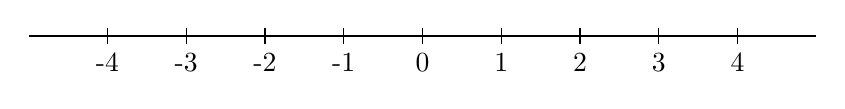
\begin{tikzpicture}
\rm \draw[thick] (-5,0)-- (5,0);
\rm \foreach \x in {-4,...,4}
\rm \draw (\x, 0.1)--(\x, -0.1) node[below]{\x};
\end{tikzpicture}
\end{figure}
idoMdu pUNARMkagaLanunx oLagoMDiruva oMdu reVKe. idanunx saMKAyxreVKe enunxtetxVve.

$0$ yiMda balagaDege iruva $1,2,3,4\ldots$ ivanunx \textbf{dhanapUNARMkagaLu} enunxtetxVve.

$0$ yiMda eDagaDege iruva $-1, -2, -3, \ldots$ ivanunx \textbf{QuNapUNARMkagaLu} enunxtetxVve.

$0$ mAtarx dhanapUNARMkavU alalx, QuNapUNARMkavU \textbf{alalx}.

$0, 1, 2, 3, 4\ldots$ ivu \textbf{pUNaRsaMKeyxgaLu}.

$1, 2, 3, 4\ldots$ ivu \textbf{sAvxBAvika} athavA \textbf{neYsagiRka saMKeyxgaLu}.

dhanapUNARMkagaLalilx $2, 4, 6, 8\ldots$ \textbf{besasaMKeyxgaLu}. aMdare {\rm 2} riMda nisheshxVSavAgi BAgavAguva saMKeyxgaLu.

dhanapUNARMkagaLalilx $1, 3, 5, 7\ldots$ \textbf{besasaMKeyxgaLu}. aMdare {\rm 2} riMda nisheshxVSavAgi BAgavAgada saMKeyxgaLu.

$4, 6, 8, 9, 12, 14, 15, 16, 18\ldots$ muMtAda saMKeyxgaLu \textbf{BAjayxsaMKeyxgaLu} ivugaLige eraDakikxMta hecucx apavataRnagaLirutatxve.

yAvudeV saMKeyxyanunx adeV saMKeyxyiMda mAtarx BAgisalu sAdhayxvAguva saMKeyxgaLu aviBAjayx saMKeyxgaLu athavA eraDeV apavataRnaviruva saMKeyxgaLige \textbf{aviBAjayx saMKeyxgaLeMdu hesaru.}

\textbf{udA}: $2, 3, 5, 7, 11, 13, 17, 19 \ldots$ {\rm 1} aviBAjayx saMKeyxyalalx {\rm 2, 3} avaLi aviBAjayxsaMKeyxgaLu {\rm 3, 5}, {\rm 11, 13} ko perxYmfsx.

$1, 4, 9, 16, 25\ldots$ muMtAda saMKeyxgaLu \textbf{vagaRsaMKeyxgaLu} aMdare oMdeV riVtiya eraDu apavataRnagaLanunx hoMdiruva saMKeyxgaLu.

$1, 8, 27, 64, 125\ldots$ muMtAda saMKeyxgaLu \textbf{Gana saMKeyxgaLu}. aMdare oMdeV riVtiya mUru apavataRnagaLanunx hoMdiruva saMKeyxgaLu.

yAvudeV sAvxBAvika saMKeyxyu tananxnunx horatupaDisi uLida apavataRgaLa motatxkekx samanAdare adu \textbf{paripUNaRsaMKeyx}.
\begin{align*}
\text{udAharaNege:}\quad  6 &= 1+2+3\\
28 &= 1+2+4+7+14\\
496 &= 1+2+4+8+16+31+62+124+248
\end{align*} 
$6,28,496\ldots$ \textbf{paripUNaRsaMKeyxgaLu}

{\rm P} matutx {\rm Q} pUNARMkagaLAdare $p/q$ rUpada saMKeyxgaLu $(q\neq 0)$ \textbf{BAgalabadhx saMKeyxgaLu}.

\textbf{udA:} {\rm 3/2, 7/4}.

${\sqrt 2}, {\sqrt 3}\ldots$ muMtAda saMKeyxgaLanunx eraDu pUNARMkagaLiMdAda BinanxrAshiya rUpadalilx bareyalu sAdhayxvilalx. ivu \textbf{aBAgalabadhxsaMKeyxgaLu}.

ivelalxvU saMKeyxgaLalilx oMdu vidhavAda neYja saMKeyxgaLu. matotxMdu riVtiyeV kalapxnA  saMKeyxgaLu. $\sqrt-1$ oMdu kalapxnAsaMKeyx {\rm Imaginary Number}. neYjasaMKeyx matutx kalapxnA saMKeyxgaLu oTuTxgUDi saMkiVNaR athavA misharx saMKeyxgaLAgutatxve. 

\chapter[A {\sl pūrva-pakṣa} of “Deep Orientalism?”]{A {\sl\bfseries pūrva-pakṣa} of “Deep Orientalism?”}\label{chapter2}

\Authorline{Ashay Naik}
\lhead[\small\thepage\quad Ashay Naik]{}

\section*{Abstract}

This paper is an attempt at a {\sl prima facie “pūrva-pakṣa”} analysis of “Deep Orientalism?\endnote{The question mark in the title of Pollock’s essay is pertinent and reflects its typically amorphous and suggestive style. Ideas are often expressed in the form of possibilities which would need to be substantiated by future research or are presumed to have been established by other scholars without specifying their argument. Grünendahl\index{Grünendahl} (2012) who refers to these discourse strategies as “desideratum scheme”\index{misinterpretation, techniques of, desideratum scheme} and “feigned factuality"\index{misinterpretation, techniques of, feigned factuality} (Grünendahl\index{Grünendahl} 2012:201), also notes derisively “the increasing tendency” in Pollock’s acolytes “to drop (metaphorically) the invertebrate question mark, as if Pollock’s amorphous presumptions\index{presumptions} had meanwhile coagulated into hard facts” (Grünendahl\index{Grünendahl} 2012:187).}” – an essay authored by Sheldon Pollock and published in {\sl Orientalism and Postcolonial Predicament (1993)} – an anthology of writings concerned with the issues facing Indian studies in the wake of the Orientalist critique – edited by Carol Breckenridge\index{Breckenridge, Carol} and Peter van der Veer\index{Veer, Peter van der}. The declared aims of Pollock’s essay are two-fold. Firstly, it seeks to analyse using the framework of Orientalism the collaboration between German Indology and the Nazi regime (1933-45), on the one hand; and the role of Sanskrit knowledge in the “pre-colonial forms of domination” in India, on the other. Secondly, in the light of the alleged realization - that both Indology itself, as well as its object of study (i.e. Sanskrit knowledge) have been deeply implicated in power - it proposes a critical Indology for the future that will be resistant towards imperialism, or at least not act in collaboration with it. Thus, there is a descriptive and a prescriptive component to Pollock’s essay. The purpose of this {\sl pūrva-pakṣa} is, firstly, to explain the comparative morphology of domination attempted by Pollock and expose its limitations; secondly, to interrogate the implications of the critical Indology proposed by Pollock for the study of the Sanskritic heritage. Although Pollock has not stated it explicitly as the objective of his essay, it is alleged by some that he seeks to establish a causal connection between Sanskrit thought and the forms of domination evident in colonialism\index{colonialism} and Nazism\endnote{Consider, for example, the section “Blaming Sanskrit for Nazism” in Malhotra (2016). Also, the editors of Orientalism and Postcolonial Predicament admit: “Sheldon Pollock [shows] that there are important family resemblances between precolonial Brahmanical discourse and Orientalist scholarship. Pollock argues that the German Orientalists took a feature of Brahmanical discourse, namely its distinction between Aryans and non-Aryans, as ‘civilized’ and ‘uncivilized’ respectively, and applied this distinction to their own society in their attempt to define the Jews as non-Aryan” (Breckenridge and Veer, 1993).}. The {\sl pūrva-pakṣa} will also investigate this allegation and discuss how the comparative morphology of domination makes such a reading ineluctable even if it may not be the express intent of the author himself. 


\section*{Introduction}

Pollock announces at the outset that his essay attempts to bring together German and Sanskrit knowledge-power nexuses\index{knowledge-power nexuses} within the framework of “Orientalism”\index{Orientalism} – the prototypical knowledge-power nexus which interrogates the collaboration between British Orientalism and British colonialism\index{colonialism} – as a result of which they get projected as “Orientalisms” in their own right. And in conclusion, he reflects on the challenges and promises of a new Indology in the wake of the transcended “Orientalist” one, which, inasmuch as it will be driven by American scholars like Pollock, could as well be understood as American Orientalism\index{American Orientalism}. I have thus organized the {\sl pūrva-pakṣa} in terms of these four alleged forms of Orientalism – the British, the German, the Sanskrit and the American.

\section*{British Orientalism}

There was a time when the concept of Orientalism meant simply the study of Asian languages and cultures but Edward Said\index{Said, Edward} (1978) gave the term a polemical twist while yet retaining its original sense and this inversion has been the cause of great confusion\endnote{Phillip (2014) declares: “It must be said at the outset that few specialists in Middle Eastern or Asian studies have been persuaded by Said’s appraisal of scholarly endeavours by academic Orientalists. Indeed, his book has been found to be riddled with errors, flagrant omissions, and drastic overgeneralizations.” See Phillip (2014:208-09) for a bibliography of general critiques of Said’s Orientalism. An excellent resource on the topic is the chapter Said’s Orientalism: a book and its aftermath in Lockman (2004) which gives a summary of the book and the controversial exchanges which followed its publication.} which is evident in Pollock’s essay as well. 

\subsection*{Three Senses}\index{Orientalism, three senses of}

Said offers at least three “interdependent” meanings of Orientalism\index{meanings of Orientalism}:
{\eleven
\renewcommand\theenumi{\alph{enumi}}
\renewcommand\labelenumi{(\theenumi)}
\begin{enumerate}
\itemsep=0pt
\item Anyone who teaches, writes about, or researches the Orient $\ldots$ either in its specific or its general aspects, is an Orientalist, and what he or she does is Orientalism.
\item Orientalism is a style of thought based upon an ontological and epistemological distinction made between “the Orient” and (most of the time) “the Occident.”
\item Taking the late eighteenth century as {\sl a very roughly defined starting point} Orientalism can be discussed and analysed as the corporate institution for dealing with the Orient – dealing with it by making statements about it, authorizing views of it, describing it, by teaching it, settling it, ruling over it: in short, {\sl Orientalism as a Western style\index{Indology, as a Western discipline} for dominating, restructuring, and having authority over the Orient}. (Said\index{Said, Edward} 1978: 2-3, italics mine)
\end{enumerate}}
Right off the bat we can see that in the first two meanings we are talking about Orientalism as general and trans-historical, while in the third it comes across as specific and historical. The former is purely epistemological and covers the whole gamut of what has been said by the West about the East as an entity different from itself right from the time of the ancient Greeks. The latter, on the other hand, is heavily implicated in power\index{power, political}, sponsored by power\index{power, political} and intended to secure and expand power\index{power, political}. 

Said has not distinguished between these two processes of knowledge production and this apparent oversight is what lies, in my view, at the heart of all the controversy surrounding the concept of Orientalism. 

\subsection*{Three Scopes}

Corresponding to the three meanings of Orientalism\index{three meanings of Orientalism}, Said also provides three different scopes for the knowledge which can be considered Orientalist\index{Orientalism, three senses of}. Thus, at one point he says:
\begin{myquote}
Strictly speaking, Orientalism is a field of learned study. In the Christian West, Orientalism is considered {\sl to have commenced its formal existence} with the decision of the Church Council of Vienne\index{Church Council of Vienne} in 1312 to establish a series of chairs in “Arabic, Greek, Hebrew, and Syriac at Paris, Oxford, Bologna, Avignon, and Salamanca” \hfill(Said 1978:49-50, italics mine).
\end{myquote}

This agrees well with the first meaning of Orientalism given above. Further, with regards to the second meaning of marking a distinction between the Orient and the Occident, he says:
\begin{myquote}
A very large mass of writers $\ldots$ have accepted the basic distinction between East and West as the starting point for elaborate theories, epics, novels, social descriptions, and political accounts concerning the Orient, its people, customs, “mind,” destiny, and so on. This Orientalism can accommodate Aeschylus, say, and Victor Hugo, Dante and Karl Marx.~\hfill(Said 1978:2--3)
\end{myquote}
\newpage

This suggests that even ancient Greek works such as produced by Aeschylus can be regarded as Orientalist. On the other hand, with regard to the third meaning of Orientalism\index{Orientalism, three senses of} as a post-eighteenth century phenomenon linked with colonialism\index{colonialism}, he says:
\begin{myquote}
Britain and France were {\sl the pioneer nations in the Orient and in Oriental studies} $\ldots$ [and] these vanguard positions were held by virtue of the two greatest colonial networks in pre-twentieth-century history~\hfill(Said~1978:17,~italics~mine).
\end{myquote}
\smallskip

When we consider Said’s assertion that all the three meanings are “interdependent” it becomes evident that {\sl all} the knowledge which Europe has produced about the Orient, from the beginning of its history, is Orientalist in his view i.e. tainted by a lust for domination and asseverated from a position of superiority. I think he has concentrated specifically on British and French Orientalism in the colonial period because (to use Pollock’s own eloquent words) “it offers an extreme and often transparent instance of knowledge generating and sustaining power and the domination that defines it” (Pollock 1993:77). In addition, it connects seamlessly with American Orientalism\index{American Orientalism} which – in my view – is the real target of his book\endnote{Anglo-French Orientalism\index{Anglo-French Orientalism} also provides a neat segue to American Orientalism\index{American Orientalism}, which is the main adversary of the Arab world today. Said\index{Said, Edward} was an activist for the Palestinian cause and {\sl Orientalism} belonged to a phase when “deepening political engagement in the 1970s led him to criticize the ways in which Arabs and Muslims were often depicted in the Western media” (Lockman, 2004:183). His other books in the same period addressed “the traumatic dispossession, subordination and ongoing suppression which the Palestinians had experienced at the hands of Zionism\index{Zionism} and Israel\index{Israel}” and “what Said\index{Said, Edward} saw as distorted and pernicious US media coverage of the Iranian revolution of 1978–79 and its aftermath, and of the threat which Islam allegedly posed to the United States” ({\sl ibid}). It thus appears to me that the real target of {\sl Orientalism} was actually American Orientalism, and Anglo-French Orientalism\index{Anglo-French Orientalism} provided merely the foundation for the polemic. “From the beginning of the nineteenth century until the end of World War II France and Britain dominated the Orient and Orientalism; since World War II America has dominated the Orient, and approaches it as France and Britain once did” (Said\index{Said, Edward}, 1978:4).}. But it is evident that for Said, Orientalism is an essential feature of European knowledge production about Asia as he links it with the very character of European culture:
\begin{myquote}
It is hegemony, or rather the result of cultural hegemony\index{cultural!hegemony} at work, that gives Orientalism the durability and the strength $\ldots$ Orientalism is never far from $\ldots$ the idea of Europe, a collective notion identifying “us” Europeans against all “those” non-Europeans, and indeed it can be argued that the major component in European culture is precisely what made that culture hegemonic both in and outside Europe: the idea of European identity as a superior one in comparison with all the non-European peoples and cultures. There is in addition the hegemony of European ideas about the Orient, themselves reiterating European superiority over Oriental backwardness\index{Oriental backwardness}.\hfill (Said 1978:7)
\end{myquote}

This detour into Said’s {\sl Orientalism} was necessary to clear up some of the confusion that confronts us in Pollock’s essay right at the beginning. Pollock (1993) has understood Orientalism only in terms of its third meaning given above i.e. as a process of knowledge-production necessarily connected with colonialism\index{colonialism}. He has therefore felt it necessary to make adjustments to this concept so that it can include German Orientalism and Sanskrit\index{power, Sanskrit as a source of} knowledge, neither of which were involved in colonialism\index{colonialism}. In the case of the former, he suggests that its vector should be conceived as directed inwards “towards the colonization\index{colonization} and domination of Europe itself” (Pollock 1993:77) while, to accommodate the latter, Orientalism should be understood simply as a “discourse of power that divides the world into ‘betters and lessers’ and thus facilitates the domination $\ldots$ of any group” {\sl (ibid)}. Having thus over-generalized (and consequently trivialized) the scope of Orientalism to include knowledge produced in the service of any and every kind of domination, he suggests that “Orientalist constructions in the service of colonial domination may be only a specific historical instance of a larger, transhistorical, albeit locally inflected, interaction of knowledge and power” (Pollock 1993:76).

These two adjustments suggested by Pollock to the concept of Orientalism – the multi-directionality of its vector and its trans-historicization\index{trans-historicization} to include any discourse about “betters and  lessers”– are both misleading in my view, and arise from his failure to understand Said’s\index{Said, Edward} thesis, as outlined above. This is because Orientalism, according to Said\index{Said, Edward}, was always trans-historical and yet exclusively European. While Said is typically ambivalent about his exclusion of German Orientalism\endnote{Pollock (1993:118) claims in a footnote that Said\index{Said, Edward} has acknowledged the omission of German Orientalism in his essay {\sl Orientalism Reconsidered}\index{Orientalism Reconsidered} (1985). This is false. Quite to the contrary, he specifically informs his critics that “[problems] like my exclusion of German Orientalism, which no one has given any reason for me to have included – have frankly struck me as superficial or trivial, and there seems no point in even responding to them” (Said\index{Said, Edward} 1985:90).}, his central point was: “German Orientalism had in common with Anglo-French and later American Orientalism\index{American Orientalism} $\ldots$ a kind of intellectual {\sl authority} over the Orient within Western culture” (1978:19, italics original). Ultimately Orientalism is all about the {\sl authority} which the West has wielded against the East right from the very start, as a result of which, in Said’s view, the whole corpus of European knowledge about the Orient stands implicated as Orientalist. 

Pollock’s fundamental error, as of most readers of Said, is that they focus on the connection forged by the latter between Anglo-French Orientalism and Anglo-French colonialism\index{colonialism} and then wonder what to make of the Orientalisms of other European nations whose colonial enterprise was relatively limited. But one doesn’t have to go looking for the {\sl real} subject peoples of a given Orientalism such that if one cannot be found externally, then one would need to be conceived of internally, as Pollock has done in the case of German Orientalism. For Said, Orientalism was already a trans-historical European phenomenon. The Anglo-French colonialism\index{colonialism} was only a local inflection (to borrow Pollock’s term), a historical moment when the sense of domination inherent in Orientalism came into contact with real domination in the form of colonialism\index{colonialism}. But what Said\index{Said, Edward} is telling us is that that sense of domination over the Orient was always there right from the time when Europe conceived of itself as different and as superior to the Orient. The actualization of this hegemony in the form of Anglo-French colonialism\index{colonialism} only provides a fruitful ground for a study of how it shaped real domination but it does not need colonial actualization for its existence because it has always been there as “the major component in European culture.” When Germans began their study of the Orient, they did it in the same Orientalist way as the English and the French. They also objectified an ‘Orient’ and asserted their superiority over it by claiming their ‘knowledge’ of it as authoritative. This is what, according to Said\index{Said, Edward}, makes their scholarship Orientalist (in the polemical sense).


Given the exclusively European connotations of Orientalism, it cannot be universalized to include all discourses about “betters and lessers” and thus extended to Sanskrit knowledge. Said\index{Said, Edward} (1989:208) himself has used this phrase specifically to refer to the divide that yet separates the colonized\index{colonization} from their erstwhile colonizers even after the end of colonialism\index{colonialism}. Its over-generalization leads not only to loss of historical specificity (for which Pollock duly apologizes in the essay) but even more importantly, cultural specificity – the hegemony of European epistemological categories. This is not to suggest that discrimination is not to be found in Sanskrit knowledge but it would have to be understood in the specific context of Indian culture. To regard it as Orientalist is to make the error that the knowledge, and its effects, produced by a {\sl brāhmaṇa} out of a sense of superiority over the {\sl śūdra} or the {\sl mleccha}, are analogous to the knowledge, and its effects, produced by a European out of a sense of superiority over the Oriental.

None of the foregoing – I should concede in the end – should be read as a defence of Said’s\index{Said, Edward} {\sl Orientalism} from Pollock’s distortion. My point is simply that if one does use the Saidian thesis as a point of departure – as Pollock clearly does – then one cannot make the kind of adjustments he suggests, to attain the goals which he desires. In my view, both Said’s {\sl Orientalism}(1978) and Pollock’s {\sl Deep Orientalism?}(1993) suffer from the same pathology of a hermeneutic of suspicion taken to an excess. As Marchand\index{Marchand, Suzanne} (2009: xxvi) has expressed it passionately in her defence of German Orientalism against the Saidian thesis:
\newpage

\begin{myquote}
I find presumptuous and rather condescending the conception $\ldots$ that all knowledge is power, especially since the prevailing way of understanding this formulation suggests that power is something sinister and oppressive, something exerted against or over others. Of course, knowledge can be used in this way, but knowledge as understanding can also lead to appreciation, dialogue, self-critique, perspectival reorientation, and personal and cultural enrichment. Oriental studies did partake of and contribute to the exploitation and “othering” of non-westerners $\ldots$ but it also has led to positive outcomes $\ldots$ and I cannot subscribe to a philosophical stance that suggests that such things do not motivate or characterize the pursuit of knowledge.
\end{myquote}
\vskip -40pt


\section*{German Orientalism}\index{German Orientalism}
\vskip -3pt

German Indology is depicted by Pollock as having  proceeded along two lines – a romantic quest for identity and a scholarship that privileged scientific methods {\sl (Wissenschaft)\index{Wissenschaft}} – which interpenetrated in the period of Nazi  Germany to become its intellectual foundation. He then offers some particular instances of contributions made by Germany Indologists such as Walther Wüst and Erich  Frauwallner and the investments made by Nazi Germany in their field of study. All the data provided by Pollock to construct this narrative has been disputed by Grünendahl\index{Grünendahl} (2012); and to avoid prolixity, I will not repeat his meticulous analysis here but only point out his conclusion which is that “Pollock’s master narrative $\ldots$ rest[s] on unsubstantiated claims, presumptions\index{presumptions} and misrepresentations”  (227). Instead, I will pursue a different strategy.

The connection Pollock has attempted to forge between German Indology and Nazi Germany betokens the methodological problem of his essay. Two diverse strands are here brought into juxtaposition with each other to erect the  façade of mutual reinforcement and affirmation without paying much attention to the larger whole of which they were constituent parts. This approach suffers from the problem of missing the forest for the trees by its exclusive focus on the mere trees – the inter-relationship between German Indology and Nazi Germany. However, when we do switch our attention to the forest, we realize how vast and complicated it is such that the role of German Indology becomes hardly discernible, which explains why it gets barely a mention in the historiography\index{historiography} of this period,  notwithstanding its colossal size, given the epochal consequences of Nazi Germany. It is impossible for me to contextualize within the limits of this paper in detail either German Indology or Nazi Germany; and what follows is merely a threadbare account of the reflection of various experts on this subject but hopefully it should be enough to put their interrelationship in a proper perspective.

We will focus on two areas which are of central concern in Pollock’s essay: the discourse about “betters and lessers,” which in this case takes the form of a dichotomy between Indo-German Aryan\index{Aryan} and Semite, and the inward vector of its domination which makes it “Orientalist.” First of all, we may note that Thomas Trautmann\index{Trautmann, Thomas} (1997:211-16) and Edwin Bryant\index{Bryant, Edwin} (2001:60-2) have persuasively argued against Max Müller’s interpretation of the Dasas/Dasyus\index{Dasas/Dasyus} as a nose-less, black-skinned people racially different from the Aryans. As Marchand\index{Marchand, Suzanne} points out:

\begin{myquote}
Sheldon Pollock’s argument in his essay “Deep Orientalism” that some of the racism in the term “Arya” was already imbedded in ancient Indian texts\index{texts (Sanskrit/Indic)} has been modified by Bryant and Trautmann, who have shown just how much “reading in” was necessary to wrench a racial contest between higher, lighter people, and lower, darker ones out of the ancient Indian texts”\hfill (Marchand 2009:128). 
\end{myquote}

On the other hand, antisemitism\index{anti-Semitism} has been a characteristic feature of European culture since ancient times. What we find in the modern period is only the rationalist and racist variety of an antisemitism\index{anti-semitism} which had prevailed in Europe in the Christian and pagan times as well. The roots of modern antisemitism\index{anti-semitism} lie not in German Indology but in the views of Enlightenment philosophers such as Voltaire\index{Voltaire}, whose ire against Judaism\index{Judaism} was a subset of his antipathy towards the Church and it is this dissatisfaction with Semitic\index{Semitic} religion which led to his projection of Vedic thought as a viable alternative and of the mythic Aryan Brahmin\index{Aryan!Brahmin} as its ideal practitioner, who was a foil against both the “plagiarist” Jew and the “degenerate” Indian (Figuera\index{Figuera, Dorothy} 2002:10ff). While Christianity was denounced, antisemitism\index{anti-semitism} survived because its pagan variant was recalled through the discovery of Greco-Roman knowledge. 
\begin{myquote}
By bringing classical antisemitism\index{anti-semitism} into the post-Christian rationalist thought of the eighteenth and nineteenth centuries, Voltaire enabled it to be grafted on to medieval Christian stereotypes, providing a new, international, secular anti-Jewish rhetoric\index{anti-Jewish} in the name of European culture.\hfill(Hellig\index{Hellig, Jocelyn} 2003:271)
\end{myquote}
\medskip

The cause of a German nationalism fostered by Johan Gottfried Herder’s\index{Herder, Johan Gottfried} idea of a {\sl Volksgeist\index{Volksgeist}} (a national spirit or genius) and the alleged superiority of Aryan languages\index{Aryan!languages} over Semites, and hence of their speakers, as proposed by German Indologists such as Friedrich Schlegel\index{Schlegel, Friedrich von} and Christian Lassen\index{Lassen, Christian} were important but not the only factors favouring antisemitism\index{anti-Semitism} in this period. The French theologian Ernest Renan\index{Renan, Ernest} divested Jesus of his Jewishness and made him an Aryan\index{Aryan} figure. He declared himself to be the first at having recognized the superiority of the Indo-European over the Semite race (Hellig\index{Hellig, Jocelyn} 2003:276). Another Frenchman, Gobineau\index{Gobineau} contributed significantly to the development of race theory but was not himself anti-Jewish\index{anti-Jewish}. His work, however, proved influential to the promotion of German antisemitism\index{anti-semitism} through Richard Wagner\index{Wagner, Richard} and Houston Chamberlain\index{Chamberlain, Houston}. Likewise, with “the publication of Darwin’s ideas in 1859 $\ldots$ the biologist Ernst Haeckel\index{Haeckel, Ernst} $\ldots$ became Germany’s chief apostle of social Darwinism popularizing Darwin’s ideas by applying them to the development of civilization” (Hellig\index{Hellig, Jocelyn} 2003:280-1). Thus, we find that in the nineteenth century German Indology was only one of diverse fields – nationalism, race theory, Christian historical criticism, Darwinism – which were developing independently all over Europe and nourishing German antisemitism\index{anti-semitism} in their own way. Further, German Indologists were not the only “bad” guys: “contributions to racist antisemitism came from many sources – professors, journalists, clergymen, statesmen, philosophers – and in Germany the antisemitic movement took to the streets, reaching a climax in 1881” (Hellig\index{Hellig, Jocelyn} 2003:271). 

Pollock mentions in passing that the dichotomization between Indo-German Aryan\index{Aryan} and Semite was “called into being by the social and economic emancipation of Jews” (Pollock 1993:82) but immediately suggests that it was “Orientalist” knowledge which made it possible. Thus, he ignores the problems relating to Jewish emancipation\index{Jewish emancipation} as the cause of antisemitism. Jewish emancipation refers to the process of integrating Jews into the wider Christian society which occurred in light of the egalitarian ideals of Enlightenment. Previously, they held the status of tolerated aliens living on the fringes of society as self-governing communities. But emancipation carried the cost of relinquishing their Jewish particularities and adopting the cultural norms of Enlightenment society (Hellig\index{Hellig, Jocelyn} 2003:256ff). While the Jews did enter into public life and began to occupy prominent positions as equal citizens, they were unwilling or unable to cease being a distinctive community unto themselves – a nation within a nation – which was unacceptable, especially in Germany where nationalism came to be shaped not through fulfilment of rational obligations, but through participation in the Romantic ideals of the inner spirit of the {\sl Volk}. The theorization of a racial divide between Indo-German Aryans\index{Aryan} and Semites in this period was problematic not so much for the “Orientalist” inferiorization\index{inferiorization} of the latter – since in European history the Jews have always been an inferiorized people. It is only when this inferiorization took on a racial colour i.e. when the inferior qualities attributed to the Jews came to be seen as their immutable racial traits\index{racial traits} that it became evident that emancipation could locate them within German society as equal citizens but never integrate them as such. These two limitations – adherence to their unique cultural identity on the part of the Jews and racial antisemitism on the part of the Germans – made their expulsion from the body politic seem necessary to Germans such as Hitler\index{Hitler, Adolf}; and when no nation showed willingness to grant them refuge\endnote{“Annihilation\index{annihilation} was arrived upon only after the failure of other methods, such as boycott, emigration, legislation and Aryanisation\index{Aryanisation}. Proponents of the Functionalist\index{functionalist} view argue, for example, that the Nazis\index{holocaust, Nazi} were content to be rid of the Jews through emigration until as late as 1941. The refusal of most of the rest of the countries of the world to take in the Jews gave Hitler\index{Hitler, Adolf} the green light” (Hellig 2003:44).}, total annihilation\index{annihilation} became the final solution of the Jewish question. One way to understand this problem of Jewish emancipation is to note that the earlier – Christian – understanding of the Jews, instituted a division between “betters and lessers”; and this, preposterous as it may sound, would have to be read as a kind of “Orientalism,” if we follow Pollock’s definition of the term. On the other hand, Jewish emancipation was an attempt to make them a “better”\endnote{As Hellig (2003:258) puts it so eloquently: “For Jews to obtain the ‘ticket of entrance’ to gentile society, as the young Heinrich Heine put it, they had to be made ‘better’ in some way.”} people; and what we discern is that such betterment comes at a steep cultural cost, which, if one is not willing to fully pay, transforms one from a tolerated, albeit inferiorized, outsider into an “abject” insider\index{abject insider@“abject” insider}\endnote{The term “abject” in apposition to “subject” and “object” is borrowed from Kristeva. For its application to the Jews in modern Germany, see Fitzpatrick (2008:477).}; one who therefore comes to be seen as so dangerous as to be considered deserving of total annihilation\index{annihilation}. These are the kind of complexities involved in the inter-relationships of human groups which get glossed over by Pollock’s ridiculous adaptation of Orientalism.

Pollock has referred to “the legitimation of genocide”\index{genocide, legitimation of} as the “ultimate ‘Orientalist’ project”\index{orientalist project} (Pollock 1993:96) but as the foregoing paragraphs show “Orientalism” cannot even be regarded as a primary factor in the rise of modern antisemitism, which in turn cannot be regarded as a sufficient condition for the Holocaust. Pollock only pays lip service to the difference between Functionalist\index{Functionalist} and Intentionalist\index{intentionalism/intentionalist} (Pollock uses the term “idealist”) approaches\index{approaches} in Nazi\index{holocaust, Nazi} historiography\index{historiography} (1993:88). His contention that Intentionalist views “seem to have gained at least parity in current re-thinking in the historiography\index{historiography} of the movement $\ldots$ in part attributable to the fuller history of the Holocaust now available” {\sl (ibid)} is mere hand-waving since he would like to pin the blame fundamentally on the “ideational dimension” of Orientalist knowledge. He is careful not to inform his readers that the Functionalist\index{functionalist} historians have argued that Hitler\index{Hitler, Adolf} was a lazy and weak dictator, driven by historical circumstances, and that war and genocide\index{genocide} were the result of the “cumulative radicalization”\index{cumulative radicalization} arising from the chaotic and competitive nature of the Nazi\index{holocaust, Nazi} state apparatus rather than from a specific ideology (Mason 1995:212ff). 

Matters get even more complicated as precedents to Nazi atrocities\index{Nazi atrocities} can be found not only in the pogroms\index{pogroms} of the Soviet {\sl kulaks}\index{Soviet kulaks} and the Armenians, but in the Herero\index{Herero} and Nama genocides\index{genocide, Nama} (1904--07) perpetrated by Germany itself in its South-West African colonies. There is, first of all, the controversy known as {\sl Historikerstreit} about whether the Nazi period (1933--45) should be cordoned off as a unique event in German history lest its historicization leads to the normalization and trivialization of the Holocaust, or whether it should be viewed as the end product of a way of modernization that was unique (Sonderweg\endnote{“The Sonderweg thesis, as the name suggests, emphasized that nineteenth- and early twentieth-century Germany suffered the stain of a uniqueness stemming from a maimed path to modernity, a path via which Germany became not another England, the putatively normative successful nation, but a ``conservative utopia" in which liberalism was only weakly anchored. Ineluctably, this narrative suggested, by reaching its historic turning point and ``failing to turn,” Germany missed the path to modernity and was only shocked into becoming a “normal” liberal state by undergoing the purgative rigours of National Socialism.” (Fitzpatrick\index{Fitzpatrick, Matthew P} 2008:481). The thesis has been disputed in {\sl The Peculiarities of German History} by Blackbourn and Eley {\sl (ibid)}.}) to Germany and different from other European nations. There is further controversy on whether the German colonial genocide\index{genocide} is to be causally connected with the Holocaust or not and whether this connection, if accepted, should be treated as supporting the Sonderweg thesis or not. Needless to say, in none of these historiographies does German Orientalism figure anywhere at all. Fitzpatrick\index{Fitzpatrick} (2008) who has done an excellent survey of these various positions, concludes that European colonialism\index{colonialism} produced initially a hierarchical racism based on socio-political differences but as miscegenation tended to blur the difference between ruler and ruled, a biological racism\index{biological racism} arose in the colonial milieu which treated the Mischlinge\index{Mischlinge} (mixed blood) as the abject entity which polluted the self. It was this biological racism, which developed in the context of colonialism\index{colonialism}, which was exported back to Europe. While all European colonial nations were equally affected by this problem, the German case was peculiar – not necessarily due to Sonderweg – but because its defeat in the first World War brought its colonial adventure to an abrupt halt:
\medskip

\begin{myquote}
With colonialism\index{colonialism} suppressed by the victorious French and British, it was transformed into a vehicle for a hypertrophic expansionist nationalism that sought internal as well as external grounds for the catastrophic failure of the German nation-state to maintain parity with or hegemony over other European powers $\ldots$ Upon its return to Europe, expansionism\index{expansionism} predicated on racial difference was fundamentally altered, with “inner,” biological categories of difference inferred in a colonial discourse tailored for Europe, where external markers of racial difference were not apparent and would therefore not serve the purpose of imperial social stratification\index{social stratification}. New biological categories were consolidated – a biologically inferior alterity – the “Asiatic” Slav, and an abject, polluting, debased German self, the biologically deficient but nonetheless assimilated “Germanic Jew” $\ldots$ One was to be conquered and ruled, even at the risk of a war of annihilation\index{annihilation}. The other was simply to be eliminated ruthlessly, expelled from the body politic

\hfill(Fitzpatrick\index{Fitzpatrick, Matthew P} 2008:500-1).
\end{myquote}

This is exactly the same as the inward vector of German domination specified by Pollock but the various scholars whose views Fitzpatrick has summarized – Jürgen  Zimmerer, Isabel Hull, Benjamin Madley, Pascal Grosse,  Hannah Arendt, and others – have traced the problem to German colonialism\index{colonialism!Nazi/German} and its military competition with  other European powers, rather than to German Orientalism. What becomes evident from the foregoing is that the history of modern Germany which forms the overarching context of German Indology is a highly complex subject and a myriad factors have contributed to the rise of Nazi Germany and its agenda of war and genocide\index{genocide}. By completely ignoring this context and fixating upon German Indology alone and the collaboration between some German Indologists and the Nazi regime, Pollock misleads his readers into ascribing it an exaggerated role in the history of Nazism. But maybe that is his goal – not so much to incriminate German Indology itself as the Sanskrit knowledge which was its object of study.

Pollock (1993:83) suggests that in the Nazi period, the two limbs of German Orientalism viz. romanticism and {\sl Wissenschaft}, merged to become the official worldview of the state and “fostered the ultimate ‘Orientalist’ project\index{orientalist project}, the legitimation of genocide.” What made this interpenetration possible was, according to him, the conceptual framework of a facts-based, value-free, objective scholarship  which sought to transcend political values: 

\begin{myquote}
It offers a superb illustration of the empirical fact that disinterested scholarship in the human sciences, like any other social act, takes place within the realm of interests; that its objectivity is bounded by subjectivity; and that the only form of it that can appear value-free is the one that conforms fully to the dominant ideology, which alone remains, in the absence of critique, invisible as ideology
\hfill(Pollock 1993:96).
\end{myquote}
\medskip

This denunciation of objective scholarship and the corresponding valorisation of a “morally sensitive scholarship” shows that for Pollock it is not so much important for research to be  evidence-based as it should be engaged in the politics of the underdog such as “giving priority to what has hitherto been  marginal, invisible and unheard” (Pollock 1993:114). This view, which suggests that knowledge is ineluctably political, and  therefore necessarily biased, as a result of which morality demands that it should be employed to favour the weak, explains the motivation behind some of his other works such as ‘political philology’\index{political philology} as well as points to the fundamental weakness in his overall scholarship.
\vskip 2pt

First of all, there is the contrary opinion that knowledge is not necessarily political – passionately articulated by Marchand (2009: xxvi) as stated above. Secondly, and more importantly, in the specific context of {\sl Wissenschaft}, Pollock’s remonstrations against objective scholarship make no sense at all. Romanticism, which arose out of a sense of alienation and loss, prioritized emotion or will over reason, which was advocated by the Enlightenment. Objective scholarship essentially means that reason should be independent of will. If reason became subservient to will under the Nazi regime, as is evident from its promotion of “pseudo”-science aimed towards the achievement of preconceived results, it was not because reason was not aware of the power of will, as Pollock suggests, but because it was self-consciously brought into subservience of the will by the Nazi regime. Hitler\index{Hitler, Adolf} belaboured that the German antipathy towards the Jews was emotional and needed to be understood scientifically. Accordingly, he advocated a “scientific antisemitism”\index{Hitler, scientific antisemitism@Hitler, "scientific antisemitism"} or an “antisemitism of reason” (Steinweis\index{Steinweis} 2006:7). To put simply, Hitler’s point was that “will” remains ineffective unless reason serves as its instrument. It is interesting to note that Pollock is making the same point albeit on the ground that knowledge is ineluctably political i.e. to say, reason is necessarily subservient to will and so should not pretend to take an independent stand. Furthermore, Hitler too would claim that he was advocating a “morally-sensitive scholarship”\index{morally-sensitive scholarship} since, from his perspective, he was only trying to save Germany from being destroyed from within by the “Jewish bacillus”\index{Jewish bacillus} (Fitzpatrick\index{Fitzpatrick, Matthew P}, 2008:477).

In conclusion, the superficial manner in which Pollock has dealt with the subject of German Indology and the Nazi regime – raising the issue of an allegedly objective scholarship and lengthy pronouncements by some Indologists sympathetic to the Nazi cause – suggests to me that he is not genuinely interested in understanding this complex and tragic chapter in German history whose many dimensions I have sought to outline above. Instead, it appears that the objective is to use German Orientalism as a bridge between British and Sanskrit Orientalism whose affinities are otherwise not at all sensible given that the former was engaged in the study of colonized people for the purpose of colonial rule, while the latter was nothing of the kind. The aim of projecting German Orientalism as knowledge sponsored by a state for the domination, oppression and extermination\index{extermination} of its own citizens, facilitates the conception of Sanskrit knowledge along similar lines and thus makes it amenable to a theorization as an epistemological tool meant for political ends.

\section*{Sanskrit Orientalism}

In order to theorize Sanskrit knowledge as a form of “pre-Orientalist Orientalism” collaborating with a “pre-colonial colonialism\index{colonialism},” Pollock (1993:96 ff.) disputes the post-colonialist view that Brahmanical texts\index{texts (Sanskrit/Indic)} were elevated to a legal authority under colonial rule and their formulations thus acquired an unprecedented hegemonic form. His contention is that such a transformation had already occurred in the production of the commentaries and digests on the {\sl dharma-śāstra-s}\index{dharma-śāstra} – the {\sl dharma-nibandha}\index{dharma-nibandha} genre – during the eleventh and twelfth centuries CE. He specifically points out the Hindu rulers of this period who sponsored these works and refers to their authors as Indian “Orientalists” (Pollock 1993:98). He attempts to rationalize this cultural production by suggesting that it occurred as a “special reaffirmation of {\sl dharma}”\index{dharma} in response to the Turkish invasion. He outlines the various restrictions imposed on the {\sl śūdra-s} in the {\sl dharma-śāstra-s}, including denial of Vedic knowledge, as an instrumental use of knowledge for the purpose of domination.
\newpage

The fact that the {\sl dharma-śāstra-s} conceive of people belonging to different {\sl varṇa-s}\index{varṇa} as consisting of different essential natures and assigns them, accordingly, different sets of privileges and obligations is common knowledge. But to reduce this schema to a mere form of domination without supplying the necessary context – as Pollock attempts to do – becomes just as problematic as in the case of German Orientalism, explained in the previous section. As far as the knowledge aspect is concerned, one is required to study the {\sl dharma-śāstra-s} holistically, as say Kane or Lingat\index{Lingat, Robert} has done, and if the dimension of power is of interest, then it would be necessary to consider its competition with other sources of power, mainly derived from custom, in its attempt to transform itself into law – the instrument of legitimate coercion in society. However, just as in case of his study of German Orientalism, Pollock has done neither of the two. On the one hand, he remains fixated on the apparent iniquities of {\sl śūdra-dharma}, while on the other, he considers random statements of {\sl varṇa} hierarchy as “dreams of power” with effective bearing on reality by the mere virtue of their having been dreamt (Pollock 1993:102-3).
\vskip 2pt

It was the British judges – in 19$^{\rm th}$ century India - who faced the full brunt of the problem when they allocated a juridical character to the {\sl dharma-śāstra-s}. Undoubtedly the pronouncements of the {\sl dharma-śāstra-s} were meant for gain of spiritual merit but to what extent did they acquire the force of law such that they could assume a form of domination in pre-colonial history? It would appear that even pronouncements that were juridical in character i.e. pertaining to {\sl vyavahāra}, carried a dharmic rather than a legal force. Having assessed the debates on the issue between the colonial judges, Lingat\index{Lingat} (1973) concludes:
\smallskip

\begin{myquote}
The written law of the śāstras and the customary laws of the different groups of humanity thus existed side by side, equally respected though often in notable disagreement with each other. The former acted upon the latter and restricted its mobility; but the latter also acted upon the former through the medium of interpretation. The result was an extremely variable and diverse law\hfill(Lingat~1973:141-2).
\end{myquote}
\smallskip

The pre-colonial Indian judge, then, played the role of an arbitrator “who had the power to apply as the case demanded the law of the holy {\sl ṛṣi-s} or the custom of ancestors” (ibid). Given its coercive nature, if law is one of the best indexes of the structure of power in society then we can see that it was a contested issue between the {\sl dharma-śāstra-s}\index{dharma-śāstra} and the customs of various local groups.

As mentioned above, in order to offer a precedent for the changes which occurred in Hindu Law in the colonial period, Pollock refers to the composition of the {\sl dharma-nibandha}-s\index{dharma-nibandha} as a sort of “pre-Oriental Orientalism” in the face of the Turkish invasion. However, systematization of the {\sl dharma-śāstra} texts\index{texts (Sanskrit/Indic)} in the form of commentaries and digests began in the ninth century with the famous gloss of Medhātithi\index{Medhātithi} on the {\sl Manusmṛti}\index{Manusmṛti} and not in response to any foreign invasion\endnote{The commentaries ({\sl bhāṣya})\index{bhāṣya@\textsl{bhāṣya}} and digests ({\sl nibandha})\index{nibandha} can be understood as narratives in the same genre. Pollock himself makes no attempt to distinguish between the two. The differencem is only that the digests arranged their material topically while the commentaries based themselves on a particular {\sl dharmaśāstra}\index{dharma-śāstra} but they too included materials from other {\sl dharmaśāstras}\index{dharma-śāstra} and sought to reconcile between them as they approached these master texts\index{texts (Sanskrit/Indic)} as a single corpus (see Lingat\index{Lingat, Robert} 1973, 107 ff).}. According to Lingat (1973:143-4) it was probably an attempt at rediscovery after a hiatus had passed since the composition of the last {\sl dharma-śāstra}-s.

In any case, these two events – the production of the {\sl dharma-nibandha}-s and the production of Indological works in the colonial period – in different times and under radically different circumstances, and in fact authored by different people – the Indians in the first case and the Europeans in the latter – can hardly be comparable. True, both involved scriptural study and validation, and both were sponsored by powers ruling in India, but that is only a superficial comparison. In the nineteenth century, we know that Eurocentric\index{Eurocentric} and Christocentric frameworks\index{Christocentric frameworks} were used in the study of Indian scriptures for the purpose of colonization and proselytization. Further, the interpretations were explicitly intended to be of juridical value to enable the colonial government to rule its Hindu subjects. On the other hand, {\sl dharma-nibandha} interpretation\index{dharma-nibandha interpretation@\textsl{dharma-nibandha} interpretation} was of an exegetical nature, using the principles of Mīmāṁsā\index{Mīmāṁsā} whose purpose was clearly to elucidate {\sl dharma} rather than law.


When it comes to Sanskrit knowledge, Pollock repeatedly uses the term “pre-colonial forms of domination” for the real nature of social power in ancient India is not known with certainty. In fact, a “detailed topography of pre-colonial domination” (1993:104) is a desideratum in his view but yet he declares in advance that it would consist of “not just the instrumental use of Knowledge (indeed, of {\sl veda}\index{Veda}) in the essentialization and dichotomization of the social order, but the very control of knowledge” {\sl (ibid)}. On the other hand, he complains that the post-colonialists, without having interrogated the forms of pre-colonial domination, accuse the British of having arbitrarily privileged the {\sl dharma-śāstra}-s over local custom. Thus, he refers to the essay {\sl Contentious Traditions: The Debate on Sati in Colonial India}\index{Contentious Traditions: The Debate on Sati in Colonial India} by Lata Mani\index{Lata Mani} in which she contends that as an effect of the colonial discourse, Brahmanical scripture came to be privileged and constituted as the authentic cultural tradition of India. His argument is that in order to prove this point, the author does not “proceed to the logically prior question, ‘whether brahmanic texts\index{texts (Sanskrit/Indic)} [have] always been prioritized as the source of law’\index{law, sources of} $\ldots$ but to ‘a careful reading of the Parliamentary Papers’ $\ldots$ [and thus] we never leave the colonial arena in pursuit of these goals” (1993:99).

However, he does not consider the fact that the reason why Mani does not find it necessary to leave the “colonial arena” is that the evidence she is looking for is covered in the texts of the colonial period where she discerns a change in the depositions made by the pundits:
\begin{myquote}
While officials treated {\sl vyavasthās}\index{vyavasthās} (the written responses of pundits to questions put to them by colonial officials on various aspects of sati) as truthful exegeses of the scriptures in an absolute sense, it is clear from reading the {\sl vyavasthās} that the pundits issuing them believed them to be interpretive\hfill (Mani 1987:133).
\end{myquote}

As Mani explains, the Parliamentary Papers show that the {\sl vyavasthās} were tentative which would imply that the pundits issuing them were being called upon to interpret scripture in altogether different ways and for unprecedented purposes: 

\begin{myquote}
In the beginning at least, the responses of pundits appointed to the court did not reflect the kind of authority that colonial officials had assumed, both for the texts and the pundits ({\sl ibid}, 149). 

By contrast there is nothing tentative about the 1830 orthodox petition; there are no qualifiers prefacing textual excerpts $\ldots$ [and the petition was noted as being] ‘accompanied by legal documents.’ Here the equation between law and scripture is complete (150). 
\end{myquote}

What Mani’s research of the Parliamentary Papers reveals is how Indians adapted themselves as they began to understand what could and could not pass muster in the new regime as legally admissible and gradually started prioritizing scripture in their legal petitions as they realized it would prove most effective with their colonial masters. It is evident from Mani’s essay that apart from Brahmanical scripture, there were other sources of law\index{sources of law} such as caste councils\index{caste!council} and customary usages, which were ignored by the colonial administrators.
\newpage

While Lingat\index{Lingat, Robert} (1973:139 ff.) explains how the British judges such as H. Nelson, District Judge in the Madras Presidency, and Indologists such as Auguste Barth sought to rectify the undue weightage they had ascribed to the {\sl dharma\index{dharma}-śāstra}-s in legal matters due to European presumptions\index{presumptions} about the operation of law, Pollock chooses to repeat the errors of the early Orientalists. He treats the restrictions on the {\sl śūdras} in the {\sl dharma-śāstra}-s\index{dharma-śāstra} as “juridical structures of inequality” (Pollock 1993:111) and speculates that “in fact, much of the discourse as we find it in the nineteenth-century Raj could easily have derived, and may have actually derived, from a text like the twelfth-century digest” (Pollock 1993:100).
\medskip

\section*{American Orientalism}\index{American Orientalism}

The purpose of Pollock’s essay is to highlight the challenges faced by an Indology confronted with the realization of its Orientalist essence and its future in a world which remains suspicious of objectivity and where critical knowledge remains subservient in unknowable ways to imperialist ambition. In the final section of his essay, titled ‘For a Critical Indology,’ Pollock explains four limitations of Indological scholarship which have become exposed in recent times and the way forward for this discipline. This discussion merits our attention because it bears repercussions for the manner in which Indological scholars will be ideally expected to approach their objects of study.
\vskip 2pt


Firstly, Indology was complicit in colonialism\index{colonialism} and Nazism but even as these forms of domination have faded away, “the rise of a new empire and its continued production and utilization of Orientalist knowledge” suggests that “neo-colonial foundations have been built in their place” (Pollock 1993:111). Without naming it, Pollock appears to be hinting at the rise of an American Orientalism\index{American Orientalism}. 
\vskip 2pt

Secondly, Pollock relates Indology to a more general “crisis of the culture of humanistic scholarship as such” (ibid). He refers to scholars in humanistic studies who collaborated directly or indirectly with repressive powers and questions the value of their scholarship to human life. Interestingly, the scholars he mentions in this context include only those who later came to be associated with fascism\index{fascism} such as Heidegger,\index{Heidegger, Martin} Paul de Man,\index{Man, Paul de} Eliade\index{Eliade, Mircea} and Dumezil\index{Dumezil}. He is careful not to draw suspicion towards Western scholarship in the humanities, which was supportive of leftist repressive powers. 

Thirdly, while humanistic scholarship in the West remains critical of the dominant regime, it is at the same time sponsored by the regime itself through its institutions. This point raised by Pollock is important because it unwittingly reveals the warped mentality which critical scholarship has assumed in our times. It is but obvious that any liberal regime will allocate space for an oppositional discourse and encourage a diverse set of ideas which will serve as a check on excess. But it is only those who enter that space not so much to offer correctives to the policies of the dominant regime but to overthrow the system in its totality, who ponder in amazement at the sponsorship they receive from it and disparage it as “domestication” and “commodification” of their knowledge. 


Finally, Pollock once again alludes to the problem of objectivity in scholarship which is readily admitted in theory but is not corrected in practice. This neatly sums up the crisis faced by the humanities in the West and it is important for Indians to pay attention to it because Indology, as a Western discipline,\index{Indology, as a Western discipline} as the application of Western theories for studying Indian texts\index{texts (Sanskrit/Indic)} and traditions, is equally affected by it.

Let us now consider the tentative solutions which Pollock has proposed to overcome the foregoing problems. Firstly, with regards to the issue of objectivity, he suggests that “we should construct perspectives that $\ldots$ would include giving priority to what has hitherto been marginal, invisible and unheard” (114). While Pollock admits the difficulties of excavating this knowledge “given the radical silencing and screening out of communities effected by ‘classical’ culture” ({\sl ibid}), what is unclear is the relation of this strategy to the problem of objectivity which as he puts it has to do with “the pre-judgments, theory-ladenness, and perspectival partiality out of and with which we perceive $\ldots$ a cultural object; the way discourses serve in class-divided societies to sustain forms of domination; the purely rhetorical (rather than ontological) status of the truth claims of historical description” (Pollock 1993:113). 


The implicit suggestion here is that since scholarship cannot be objective anyway it is best to justify it as the unworthy means to the noble end of giving voice to the “marginal, invisible and unheard.” What is disquieting is that since these voices have admittedly been “radically silenced and screened out” by the “classical” culture, their recovery will likely involve nothing more than a denigration and denunciation of the “classical” culture itself and a superimposition by contemporary thinkers of their own radical views on their objects of study. We must bear in mind that according to the standard Orientalist critique, such a dominant Sanskritic “classical” culture is itself the construct {\sl par excellence} of colonial Indology. Pollock, on the other hand, appears to be suggesting that colonial Indology privileged a Sanskritic “classical” culture that had always been dominant and what future Indology should do is privilege those cultural voices which were allegedly dominated by it. Hence his desperate attempts to “save” colonial Indology from the stigma of Orientalism i.e. from the allegation of having constructed an imagined India using a Western lens. What he is effectively saying is that colonial Indology did not err in terms of the form of the dominant Sanskritic “classical” culture which it conceived; it erred rather in perpetuating that dominance when it should have deprecated it and this is the error which future Indology should strive to rectify.  


Secondly, he points out that prior to the eighteenth century, the world system was dominated by India while Europe enjoyed a peripheral position. However, the socio-economic historiography\index{historiography} of India was geared towards explaining the causes of under-development rather than the actual developments which had occurred. In a similar manner, he suggests that “a pre-emptive European conceptual framework of analysis has disabled us from probing central features of South Asian life, from pre-western forms of ‘national’ (or feminist, or communalist, or ethnic) identity or consciousness, pre-modern forms of cultural ‘modernism,’ pre-colonial forms of colonialism\index{colonialism}” (Pollock 1993:115). 

What is assumed here is that if India was a developed economy prior to the colonial conquest then it must have analogous formulations of modernity and the purpose of Indology is to discover the Indian equivalents for those categories which qualify as modernistic in the West. This is a problematic quest because it does not seek to understand India in terms of its own intellectual categories but presumes that similar historical processes were taking place in India as in the West but got arrested due to the colonial intervention. Instead of imposing the Western forms, it seeks to activate the allegedly native forms of these historical processes. These correspondences sound eerily familiar to the manner in which developments within a Western category like ‘religion’ are mapped to Indian phenomena such that the flow “Old Testament – New Testament – Catholicism – Protestantism”\index{Protestant(ism)} becomes comparable to “Veda\index{Veda} – Upaniṣads – Brahmanism or Dharmic Hinduism\index{Hinduism} – Buddhism\index{Buddhism} and other protest movements.”


Thirdly, Pollock warns sternly against “third-worldism”\index{third-worldism} i.e. the projection of an unproblematized concept of tradition. He points out that “traditions $\ldots$ have been empires of oppression in their own right – against women, above all, but also against other domestic communities” (Pollock 1993:116). In the Indian case, he considers Sanskrit as the main agent of oppression. He understands the difficulties faced by the Western scholars in thematizing violence in traditions which have suffered at the hands of the West, but appears to condone the intervention in cases of “a culture’s failure to play by its own rules” and “evidence of internal opposition to its domination” ({\sl ibid}). Both these are problematic clauses as a loop-hole can easily be found to justify intervention through the production of “atrocity literature.”\index{atrocity literature} There is also the audacity of interventionism\index{interventionism} to consider here as if there is a mandate for Western scholars to meddle in the internal issues of “third-world” cultures. It is not clear if such a mandate is entrusted to Western intelligentsia in general with regards to all cultures, or if this is a prerogative merely of Western Indologists with regards to Sanskrit culture. What is, however, most alarming in this point is the advocacy of a {\sl prima facie} approach towards “tradition” as an “empire of oppression” rather than seeking to understand how it facilitates the maintenance of a decent society. On the other hand, we have seen in the previous point how the Indologist is exhorted by Pollock to highlight the modernistic impulses in Indian history, notwithstanding the fact that the most widespread and horrific instances of oppression in the last three centuries are to be found in modernity.

Finally, Pollock is critical of attempts at historicizing the “traditional domination as coded in Sanskrit” ({\sl ibid}). He quotes the view of a random woman who claims to submit to “the economic, social and emotional violence of Indian widowhood” on account of the {\sl śāstra-s} and a Dalit manifesto which declares the “first and foremost object of this cultural revolution” to be the liberation of every person from the “thraldom of the {\sl śāstra-s” (ibid)}. Clearly, in his view the {\sl śāstra-s} are highly oppressive in nature and their ill-effects are experienced to this day. He demonstrates no interest in verifying the allegations laid against the śāstra-s or what improvements can be done to check their excesses. If we refer to his views articulated elsewhere in the essay that “none of this palliation [of counter-movements like Buddhism\index{Buddhism} or sectarian movements like Pañcarātra\index{Pañcarātra}] makes itself felt in the totalizing constructions of the social order” (Pollock 1993:110), it is evident that he considers the situation hopeless. His intention appears to be nothing short of branding the {\sl śāstra-s} as an incurable evil and thus exhorts that “we should not resist any ‘historicization’ that serves to normalize or trivialize domination” (Pollock 1993:116).

I assume that Pollock wants to say that we {\sl should} resist ‘historicization’ and the negation is a typo because he gives here the example of {\sl Historikerstreit}\index{Historikerstreit} in which a critique was developed against the demand for a historicization of the Nazi\index{holocaust, Nazi} period. As we have noted above, in the previous two sections, understanding German Indology in the context of historical antisemitism, Nazi\index{holocaust, Nazi} Germany in the context of German colonialism\index{colonialism!Nazi/German}, and Sanskrit knowledge in the context of tension between {\sl dharma} and law, permits us to come to grips with the tragedy which overcame the Jewish people and the traditional Hindu legal system. On the other hand, to quarantine these historical moments, whether Nazi Germany or the Sanskrit culture, as if they were manifestations of some kind of an ahistorical, demonic evil, would reduce them simply to monuments of undying national shame, which has happened in the case of the former and which, it appears, Pollock would like to make happen in the case of the latter. What is ironical is that by drawing a comparison between Nazi Germany and Sanskrit culture, he accomplishes the very travesty he seeks to avoid – of normalizing and trivialising the crimes of Nazism. After all, at the core of {\sl Historikerstreit} lay precisely “the question of moral equivalence – the notion that by comparing atrocities and genocides\index{genocide}, the Holocaust is diminished through its linkage with other ‘lesser’ events” (Fitzpatrick,\index{Fitzpatrick, Matthew P} 2008:483).

Furthermore, it is hypocritical that Pollock does not find it problematic to historicize British colonialism\index{colonialism!British} by tracing its form of domination to a “pre-colonial colonialism.” In this matter, he willingly “jeopardizes the heuristic historical specificity of the very concept [of Orientalism]” on the pretext that “we may lose something still greater if not doing so constrains our understanding of the two other historical phenomenon [i.e. German Indology and Sanskrit knowledge]” (Pollock 1993:78).Yet elsewhere, in the process of criticizing the pursuit of objectivity in scholarship, he deplores “the decontextualization and dehistoricization of the scholarly act” pointing out that it “enabled some of the most politically deformed scholarship in history $\ldots$ to come into existence” (Pollock 1993:86-87).It thus appears that determining which historical events, concepts and texts\index{texts (Sanskrit/Indic)} should or should not be historicized, contextualized or, for that matter, “nuanced,” constitutes the very essence of the politics of knowledge production.

\section*{Conclusion}

The declared intent of Pollock’s essay is to extend the framework of Orientalism to include German Indology and Sanskrit knowledge and thus to depict them as forms of domination. However, the net result of this effort is to exonerate British Orientalism\index{British Orientalism} from misinterpreting and misrepresenting Sanskrit knowledge for the advancement of colonial rule, and project Sanskrit knowledge itself as a factor in the development of Nazi ideology. It is impressed upon the reader through reiteration that Sanskrit knowledge was a tool for expressing power\index{power, Sanskrit as a source of} in ancient India:
\begin{myquote}
Sanskrit knowledge\index{Sanskrit knowledge} presents itself to us as a major vehicle of the ideological form of social power in traditional India\hfill (Pollock 1993:77).
\end{myquote}

\begin{myquote}
Sanskrit was the principal discursive instrument of domination in\break pre-modern~India \hfill(Pollock 1993:116).
\end{myquote}

\begin{myquote}
[An] analysis of the object of Indology [i.e. Sanskrit knowledges] $\ldots$ as an indigenous form of knowledge production {\sl equally saturated with domination} [as Indology itself, has] important implications 

~\hfill(Pollock 1993:80, italics mine). 
\end{myquote}
However, if Sanskrit knowledge was always imbricated in power, then its projection as a form of domination in Indology cannot be treated as a distortion, which means that Indology itself cannot be considered as Orientalist in the polemical sense. Rather, it suggests that if Indological knowledge abetted in colonial domination it was because its object of study naturally lent itself to such an application for even prior to the British conquest, it was a form of exercising hegemony. Pollock admit this much as well:
\newpage

\begin{myquote}
Sanskrit and Indian studies have contributed directly to   consolidating and sustaining programs of domination. In this (noteworthy orthogenesis) {\sl these studies have recapitulated the character of their subject}, that indigenous discourse of power for which Sanskrit has been one major vehicle and which has shown a notable longevity and resilience

~\hfill  (Pollock 1993: 111, italics mine).
\end{myquote}
If the British Indologists were simply ‘recapitulating the character of their subject’ in their collaboration with colonialism\index{colonialism, British}, then it can well be said that the German Indologists were doing the same in their collaboration with Nazism. Pollock forges a connection between Sanskrit knowledge and Nazi ideology through such subliminal devices as referring, on the one hand, to the anti-Jewish\index{anti-Jewish} laws in Nazi Germany as {\sl śāstric} codifications (Pollock 1993:86) and advising, on the other hand, the intellectual-historical\index{intellectual history} study of the Sanskrit {\sl arya} in a manner analogous to the German {\sl Arier}\index{Arier@\textsl{Arier}} (Pollock 1993:107). He treats the restrictions on the {\sl śūdra}-s found in dharmic texts\index{texts (Sanskrit/Indic)} as “components of a program of domination whose true spirit we might begin to conjure with other comparable programs, such as the {\sl Arierparagraphen}\index{Arierparagraphen@\textsl{Arierparagraphen}} of the NS state” (Pollock 1993:111). His expostulation against the historicization of Sanskrit knowledge is also expressed through a reference to the {\sl Historikerstreit} debate suggesting that its form of domination be considered analogous to the Nazi regime. Sanskrit knowledges thus serve not only as a vehicle of oppression in their own right, but through British and German Indology become causal factors in colonialism\index{colonialism!British} and Nazism\index{colonialism!Nazi/German} as well. All these memes of oppression, historically associated with Western powers – British and Nazi – thus converge upon Sanskrit knowledge through Pollock’s slanderous project of the comparative morphology of domination.


\begin{thebibliography}{99}
\itemsep=2pt
\bibitem[]{chap2_item1} 
Adluri, Vishwa. (2011). “Pride and Prejudice: Orientalism and German Indology.” {\sl International Journal of Hindu Studies}. Vol.~15, No.~3 (DECEMBER 2011), 
pp.~253--292

\bibitem[]{chap2_item2}
Breckenridge, Carol and Peter van der Veer. (1993). {\sl Orientalism and Postcolonial Predicament}. University of Pennsylvania Press, Philadelphia.

\bibitem[]{chap2_item3}
Bryant, Edwin. (2001). {\sl The Quest for the Origins of Vedic Culture}. Oxford University Press: New York.

\bibitem[]{chap2_item4}
Figuera, Dorothy (2002). {\sl Aryans, Jews, Brahmins: Theorizing Authority through Myths of Identity}. State University of New York Press, Albany.

\bibitem[]{chap2_item5}
Fitzpatrick, Matthew P. (2008). “The Pre-History of the Holocaust? The Sonderweg and Historikerstreit Debates and the Abject Colonial Past.” 
{\sl Central European History}. Vol.~41, No.~3 (Sep., 2008),\break pp.~477--503

\bibitem[]{chap2_item6}
Grünendahl, Reinhold (2012). “History in the Making: On Sheldon Pollock’s “NS Indology” and Vishwa Adluri’s “Pride and Prejudice.”” 
{\sl International Journal of Hindu Studies}. Vol.~16, No.~2 (AUGUST 2012), pp.~189--257.

\bibitem[]{chap2_item7}
Hellig, Jocelyn (2003). {\sl The Holocaust and Antisemitism: A Short History}. Oneworld Publications: Oxford, England.

\bibitem[]{chap2_item8}
Lewis, Bernard (1993). {\sl Islam and the West}. OUP: New York.

\bibitem[]{chap2_item9}
Lingat, Robert (1973). {\sl The Classical Law of India} (tr.\ J. D. M. Derrett). University of California Press, Berkeley and Los Angeles, California. 

\bibitem[]{chap2_item10}
Lockman, Zachary (2004). {\sl Contending Visions of the Middle East: The History and Politics of Orientalism}. Cambridge University Press.

\bibitem[]{chap2_item11}
Malhotra, Rajiv (2016). {\sl The Battle for Sanskrit}. Harper Collins, India.

\bibitem[]{chap2_item12}
Mani, Lata (1987). {\sl Contentious Traditions: The Debate on Sati in Colonial India}. Cultural Critique, Autumn 1987, pp.~119--156.

\bibitem[]{chap2_item13}
Marchand, Suzanne (2009). {\sl German Orientalism in the Age of Empire}. Cambridge University Press: New York.

\bibitem[]{chap2_item14}
Mason, Timothy (1995). {\sl Nazism, Fascism and the Working Class}. Cambridge University Press: Cambridge.

\bibitem[]{chap2_item15}
Phillips, Kim (2014). {\sl Before Orientalism: Asian Peoples and Cultures in European Travel Writing}, 1245--1510. University of Pennsylvania Press: Philadelphia.

\bibitem[]{chap2_item16}
Pollock, Sheldon (1993). “Deep Orientalism? Notes on Sanskrit and Power Beyond the Raj” (pp.~76--133) in {\sl Orientalism and Postcolonial Predicament} (Ed.) Carol Breckenridge and Peter van der Veer.

\bibitem[]{chap2_item17}
Said, Edward\index{Said, Edward} (1978). {\sl Orientalism}. Vintage Books: New York.

\bibitem[]{chap2_item18}
Said, Edward\index{Said, Edward} (1985). {\sl “Orientalism Reconsidered”}. Cultural Critique, No.~1. (Autumn, 1985), pp.~89--107.

\bibitem[]{chap2_item19}
Said, Edward\index{Said, Edward} (1989). Representing the Colonized: Anthropology's Interlocutors. {\sl Critical Inquiry}. Vol.~15, No.~2 (Winter, 1989),\break pp.~205--225.

\bibitem[]{chap2_item20}
Steinweis, Alan (2006). {\sl Studying the Jew: Scholarly Antisemitism in Nazi Germany}. Harvard University Press: Cambridge, Massachusetts 

\bibitem[]{chap2_item21}
Sugirtharajah, Sharada (2003). {\sl Imagining Hinduism: A Postcolonial Perspective}. Routledge: London.

\bibitem[]{chap2_item22}
Trautmann, Thomas (1997). {\sl Aryans\index{Aryan} and British India}. University of California Press: Berkeley.
\end{thebibliography}

\theendnotes

\chapter{ASaRvidAyx saMparxdAyada bagege mwlika daqSiTxkoVna - }

\begin{center}
{\includegraphics[scale=.9]{om.eps}}\\[2pt]
BUmike\\[2pt]
mUlaBUta pAThakekx hinenxle\\[2pt]
(keSxVtarx-heDatale, dinAMka 2-6-1961)
\end{center}

\noindent
(kelavu sAdhaka sherxVSaThxra apeVkeSxyaMte BAratiVya mahaSiRgaLa saMsakxqqti nAgarikate\-gaLa bagege mUla\-BUta\-vAda halavAru viSayagaLanunx kelavarigAdarU tiLisi, avaranunx mamaRjacnxranAnxgi mADabeVkeMba Ashaya\-diMda pATha mADalu udedxVshisi, adakekx hinenxleyAgi shirxV guru BagavaMtanu aMtamuRKiVkaqta daqSiTx\-yAgi\-yeV (kaNuNx tereyadeyeV) I parxvacanavanunx pUtiRyAgi naDesikoTaTxru.)


{\bigskip
\noindent
{\large\bf pAThAraMBadalilx guru mADida namana}}\label{page64}
\medskip

\noindent
veVdagaLu asurariMda rasAtalakekx oyayxlapxDalu, BagavaMtanu tananx jAcnxnarUpavAda veVda\-vanunx rasA\-tala\-diMda meVlakekx punaH taraloVsuga yAva hayavadana\-rUpa\-diMda A veVda\-gaLanunx udadhxrisidanoV, baLika matAsxyXvatAradiMda hora\-taMdanoV, aMtaha BagavaMtanige nananx pArxNa\-gaLanunx bagigxsi namasakxrisu\-tetxVne. aMteyeV veVdamAteyAgi ipapxtatxnAlukx tatatxvXgaLiMda kUDi parx\-Nava savxrUpiyAda Bagavati gAya\-tirxV\-deVvigU nananx pArxNagaLanunx bagigxsi namasAkxra mADutetxVne.

{\bigskip
\noindent
{\large\bf pAThakekx vidAyxdhideVvana hoMdANikeyirali}}\label{page64}
\medskip

\noindent
jAcnxna biVjada Ashayakekx anuguNavAgi vikAsavAguvaMte (tananx) jAcnxnavanunx\break gAyatirxV\-deVviya gaBaR\-dalilxTuTx parxpaMcavaqkaSxvAgi beLesida haMsarUpiV haya\-vadanana maDilalilx.

\begin{shloka}
`aMkeVnoVdUhayx vAgedxVviVmAcArayxkamupAshirxtaH'\label{page64, 84}
\end{shloka} 

\noindent
eMba vAkayxvu heVLuvaMte kuLitiruva sarasavxtiVdeVvigU manadaNiye namasAkxra mADi, iva\-relalxra aMtaH\-karaNavanUnx aMteyeV manakekx tegedukoMDu, adara niluvige sahajavAgi kaTaTxlapxDuva yAva viSaya\-vuMToV adelalxvU, 

\begin{shloka}
`vishovxVtitxVNaRsavxrUpAya cinamxyAnaMdarUpiNeV' |\\\label{65}
tuBayxM namoV hayagirxVva! vidAyxrAjAya viSaNxveV' ||
\end{shloka}

\noindent
eMba dhAyxnakekx viSayanAda hayavadananige haqdayxvAguvaMte irali - eMba BAvadiMda muMdina viSayavanunx (nimage pAThavAgi) iDalu AraMBa mADutetxVnapApx! kaqSANx!

{\bigskip
\noindent
{\large\bf puruSAthaRmaya - jAcnxnavaqkaSxda beLavaNige maMdirada dheyxVya}}\label{page65}
\medskip

\noindent
BUmiyalilx yAvudeV jAtiya oMdu biVjavanunx neTaTxrU A biVjada mUla\-BUtavAda Ashaya\-vanunx heVge parxpaMcitavAgi mADikoMDu vaqkaSxgaLu beLedu tananxlilx baMda PalagaLanunx loVkakekx koDu\-tatxveyoV, hAgeyeV jAcnxnateVjoVbiVjanAda saqSiTxVshana Ashayadalilxruva dhamaR athaR kAma matutx moVkaSxgaLeMba Pala\-gaLanunx biVruvaMtaha jAcnxnavaqkaSxvanunx namamx keSxVtarxdalilx neTuTx vayxvasAya mADuva udayx\-ma\-vanunx mAtarx vijAcnxna maMdiravu keYgoLuLxva pakeSxV, I modalu namasAkxra \hbox{mADida} deVvategaLa Ashayakekx viroVdha\-vAgada riVtiyalilxyeV vijAcnxna maMdiradalilx\break \hbox{kAyaRvu} naDeyabeVkAgutatxde.

{\bigskip
\noindent
{\large\bf vijAcnxna maMdirada ugama}}
\medskip

\noindent
vijAcnxna maMdiravu AraMBavAda bageyeMtu? eMbudanunx modalu nAlukx mAtu\-gaLa\-lilxTuTx, I mU\-laka oMdu BUmikeyanunx koDabeVkAgide. idakekx munanx idadx deYvada satayx\-saMkalapx, adu nananx budidhxge\- goVcara\-vAda riVti, naMtara maMdirada AkAravAgi horage kaTaTxlapxTaTx riVti, adakekx beVkAda sAdhana saM\-patutx, muMde adu beLeyabeVkAda riVti, ivugaLa bagegxyU nAlukx mAtanunx tiLisabeVkAgide. adu horagaDe beLeyabeVkAdare raMgana mUlakavAgi matutx aMta\-raMga mUlakavAgiyeV beLeyabeVkAgide. I eraDU mUlavanunx biTuTx A jAcnxnavaqkaSxda beLavaNigeyu asAdhayxvAdudeV sari. loVkadalilx yAvu\-doMdu beLeyabeVkAdarU hiMdu hiMdinadariMda guTukanunx tegedukoMDeV beLeyuvudu savxBAva sidadhxvAgide. hAgeyeV elalx\-dara vikAsavU AguvudAgide.

{\bigskip
\noindent
{\large\bf beLavaNigeya naDe}}\label{page66}
\medskip

\noindent
udAharaNege moLakeyu biVjadiMdalU, sasiyu moLakeyiMdalU muMdakekx vikAsa\-goLuLxtatxde. diV\-pada soDarU kUDa hiMdinadariMda tegedukoMDeV meVlakekx beLeyutatxde. idu hiMdinadanunx eSeTx\-SuTx tegedukoMDu meVlakekx hoVgutotxV-vikAsagoLuLxtotxV aSaTxSuTx parxkAshavu - aMdhakAra nivaqtitx\-yAgutatxde. eSeTxSuTx keLakekx hoVdare aSaTxSuTx aMdhakAra-jAcnxna saMkoVca. A riVti diVpavanunx doDaDxdu cikakx\-dAgi mA\-Dalu oMdu kiVlikeY beVku. (lAyxMpfnalilx idanUnx kANutetxVve.) idara kiVli keYyina dAvxrAneV beLakanunx horataruvudu. idakUkx batitxgU adara senxVhakUkx nikaTa saMbaMdhavide.

{\bigskip
\noindent
{\large\bf guru-shiSayxra nele}}\label{page66}
\medskip

\noindent
hAgeyeV A AdhAyxtamxdiVpada parxkAshavanunx nimamx aMdhakArada BUmiyalilx celalxbeVkAdare, adakokxM\-du manoVdhamaR, mAtu, AloVcane, vicAra elAlx beVkAguvudu. adanunx tirugisuva kiVli nAvu. hAge kiVliya sAthxnadalilx namamxnunx nililxsidedxV Adare (tamamx kaDe keY toVrisi) idanunx hiDidukoMDu meVlakUkx hoVgabahudu. hiVge tirugisi horakUkx barabahudu. idanunx hiVge mADalu obabx guru. iva\-nanunx iTuTxkoMDu shiSayxrUpadalilx niVvu ididxVri. oLage gUDhavAgiruvudanunx horakekx taralu-vayxkatxkekx taMdu tiLisalu I kiVli. idu keVvala vayxkitxyalilx nilulxva viSayavalalx. `guru' enunxvudakekx yArapApx viSaya? eMdare - parama guru. adu oLage hokukx Avarisi, tananxdeV Ada A oLa viSayavanunx hora\-paDi\-suva kAraNa ivanu guruvAgiruvanu. ivana dAvxrA niVvu A oLagiruva guruvige shiSayxrUpada\-lilxru\-viri. `shiSayxteV iti shiSayxH' adara bagegU nimagU oMdu gUDuvaMtAguva saMdhisAthxnaveV shiSayx.

{\bigskip
\noindent
{\large\bf vidAyxdhideVvariMda beLeyabeVku maMdira}}
\medskip

\noindent
satayxjAcnxnarUpiyAda vidAyxdhideVvana-BagavaMtana oMdu toDeya meVle kuLitu jAcnxnAdhideVvate\-yAda ivaLu-BAratiV deVviyU ivananunx AliMgana mADi\break\-koMDiruvudU, ivanU (hayavada\-nanU) ava\-Lanunx biDadeV hiDidukoMDu \hbox{nimamx} raMgadalilx nATayxvADalu iruva haMsAsaneyAda deVvi\-yU, hiVge obabxri\-gobabxru haqdayakekx tabibxkoMDu daqDhavAda AliMganadalilxdudx, vijAcnxnamaMdirakekx baMdA\-galU ava\-nanenxV hiDidukoMDu adeV akaSxmAle, adeV jAcnxna muderx ivugaLoDane kUDidudx, avano\-Dane kUDi\-koMDu paDedudanunx nataRna rUpadalilx toVrisutitxdAdxLe. vijAcnxna maMdiravanunx veVdikeya\-nAnxgi mADi\-koMDiruva A mAteya aBipArxyakUkx, A mAteya haqdayada kaDege manakoTaTx A hayavadanana AshayakUkx viroVdhavilalxdeV beLeyuvudAdare adu sAkASxdaBxgavaMtana adhayxkaSxteyalilx avana neVtaqtavxdalilx mAtarx beLeyutetx eMdu heVLidare sAthaRkavAda mAtAgutatxde. ilalxdidadxre nirathaRkavAgi keVvala vAyxva\-hArikavAgi nilulxtatxde.

{\bigskip
\noindent
{\large\bf AdhivAyxdhi nivAraNeyeV maMdirada guri}}\label{page67}
\medskip

\noindent
hAge sAthaRkavAgi beLeyuva jAgadalilx mAtarx guru shiSayxrige parasapxra `Enu sAvxmi'? eMba mAtige viSaya. alilx ibabxrigU javAbAdxri beVkAgutatxde. deVhadalilxruva vAyxdhiya nivAraNegAgi veYdayxnalilxge hoVgi `Enu sAvxmi pathayx' eMdu keVLikoMDu cikitAsx-pathayxgaLanunx naDesuvaMte Adhi-vAyxdhigaLeraDanUnx toDedu hAkalu BagavaMtanalilx hoVgi, `EnusAvxmi mADabeVku?' eMdu keVLikoLaLxbeVku. loVkadalilx jiVvigaLanunx kADuva jarA-rukf-BayagaLeMba Adhi-vAyxdhigaLeraDanUnx pariharisikoLuLxva saluvAgi Baga\-vaMtanAda dhanavxMtari rUpiV nArAyaNanalilxge hoVgi keVLikoLaLxbeVku.

{\bigskip
\noindent
{\large\bf BagavaMta Bagavatiyara padataladalilx avara shikaSxNadalilx beLeyabeVku maMdira}}\label{page67}
\medskip

\noindent
`sAvxmi! nanaginUnx jAcnxnavu baMdilalxvalAlx! jiVvanavu aMdhakAravAgideyalAlx; idakekxVnu mADuvu\-dapApx' eMdu avanalilx AtiRyiMda beVDikoLaLxbeVku. AdhivAyxdhihararAda veYdayxrU, AdhivAyxdhi\-gaLiMda odAdxDu\-titxruva I jiVvigaLige upacAra mADuvavarU Ada A BagavaMta-Bagavatiyaru koTaTx ceYtanayx\-satxnayxdiMda vijAcnxna maMdiravu beLeyabeVkAgideVpApx! adu avara pAdatAvaregaLaDiyalilx beLedu muMdu\-varidu, tananx kAlina meVle niMtu ADabeVkAgide. hAge vijAcnxna maMdiraveMba shishuvu beLeyabeVku. shishuvu tAyiyu koTaTx AhAra matutx manasusxgaLanunx paDedukoMDu avaLa maDilalilx shikaSxNa paDedu tananx beLa\-vaNigeya kelasa mADikoLuLxtetx. ilalxdeV hoVdare tAyi taMdeyara shikaSxNavilalxde huTiTxdedxlolxV beLedi\-dedxlolxV Agutetx. huTiTxda takaSxNa shikaSxNa paDediralu sAdhayxveV? sushikiSxtanAgalu tAyi taMdeya Asare beVku. shikaSxNaveVpaRDadeV idadxre tirxkaraNagaLalilx sArUpayxviruvudilalx. loVkadalilx kANuva tarahAvariV saMsAkxrada shishuvAgi biDutatxde.

{\bigskip
\noindent
{\large\bf nijavAda guruveV shAsatxrXyoVni}}\label{page68}
\medskip

\noindent
`BagavaMtana manasusx, BagavaMtana mAtu, BagavaMtana kAya' elalxvU AdAga mAtarx, avanu loVka\-dalilx ADi hoVda amaravAda vANi-shAsatxrX vidhi ivugaLanenxlAlx tiLi\-yalu sAdhayx. hAge veVda-veVdayx-vidhi\-gaLelalxvanUnx tanonxLageyeV jAcnxna daqSiTx\-yiMda tiLiyabalalxvanu tAneV guru shabadxkekx yoVgayxnAguvanu, ilalxdidadxre `pusatxka heVLutetx ivaru heVLidaru' enunxvaSaTxralilx mAtarx nilulxtetx.

idakekxlAlx mUlavAdudu shAsatxrXyoVniyeV. Adare A shAsatxrXyoVni\-yAdavana viSaya aneVkAneVka keYga\-Lanunx dATi baMdiruvudariMda sAMkayaRkokxLagAgide. adariMda punaH orijinalf Agi AviSAkxra\-veVpaRDabeVkAgide. idaralilx orijinalf Enu? eMbudanunx dashaRna mADikoMDiruva matutx nimamx joteyalelxV ADu\-titxruva jAcnxnavaqdadhxra saMgadiMdaleV adu horabidudx vayxkatxvAgabeVkAgide. Adadx\-riMdaleV obabxru heVLuvudU obabxru keVLuvudU beVkAgide.

{\bigskip
\noindent
{\large\bf jAcnxna mAtApitaqgaLiMdaleV beLeyabeVku}}\label{page79}
\medskip

\noindent
namageVnAdarU mAtaqBASeyalilx pitaqBAvavu vayxkatxpaDabeVkAdare - vijAcnxna maMdirada shishuvige A jAcnxna\-pitana jAcnxnamAteya rahasayxvu tiLiyabeVkAdare, niVvu nimamxlilxyeV (oLagiMda) tiLidu heVLu\-vaMtA\-darU sariyeV, athavA nimamxlilx anugarxha hoMdiruva nimagiMta modaleV tiLidavanobabxniruvudariMda avananunx keVLitiLidarU sariye. niVvU I riVtiyanenxV keVLuvireMba BAvaneyiMda hiVge heVLu\-titxdedxVne. nimagU loVkavayxvahAra tiLidide. niVvU vidAyxBAyxsa mADididxVri. Adare niVveVnAdarU nananx haqdaya\-dalilxruva jAcnxnapitananinxTuTxkoMDu keVLuvudAdare, elalxrU inUnx bahaLa tiLidukoLaLxbeVku enanxbeVkA\-gide. yAvudoV oMdu mahAshakitxya divayxshakitxya kaDeyiMda mahAparxsAda rUpavAgi idu baMdiru\-vudariMda niVvu adakekx tale tagigx adanunx PAloV mADabeVkAgide. hAgAdareVneV jAcnxnada beLavaNige.

{\bigskip
\noindent
{\large\bf maMdiradiMda yathAthaRveV beLeyabeVku}}\label{page69}
\medskip

\noindent
meDikalf seYnasxnunx barediruvudanenxV loVkada janaru Eke PAloV mADutAtxre! taMtamamx aBipArxya\-vanenxV Eke PAloV mADabAradu?, haqdayavuMTu, adakekx nAlukx bAgilide eMdeV Eke heVLabeVku? `eMTu bAgilide' eMdeVke bareyabAradu - eMdare, alilxruvudu nAlekxV, AdadxriMda, eSiTxdeyoV aSaTxnenxV heVLabeVku. hAgeyeV jAcnxniyAdavanu oLaginadanunx OdikoMDu adanunx videyxyAgi aBAyxsa mADalu horage iTaTxre adanUnx hAgeyeV ariyabeVku. hAgeyeV heVLabeVku. idu vijAcnxna maMdi\-rada javAbAdx\-riya viSaya. A shishuvoMdu beLedu videyxyeMba kaneyxyanunx maduve mADikoMDu tananx muMdina\- parxjege tananx BASeyanunx kalisabeVkAdare - A mAtaq BASeyiMda adu muMde beLeya\-beVkAdare adakekx takakx sAhitayxveV beLeyabeVku. adu jAcnxnapitana, jAcnxnamAteya AshayakakxnuguNavAgi tatasxhitavAda sAhitayxvAgi beLeyabeVkAdare, maMdirada muderxyalilx aLavaDisiruva pArxthaRnArUpavAda -

\begin{shloka}
`vishovxVtitxVNaRsavxrUpAya cinamxyAnaMdarUpiNeV |\\\label{69}
tuBayxM namoV hayagirxVva vidAyxrAjAya viSaNxveV ||'
\end{shloka}

\noindent
eMba sholxVkada aBipArxyavu heVgideyeMbudanunx tegedukoLaLxbeVku. hAge tegedukoMDAga, `upa\-deVkaSxyXMti teV jAcnxnaM\label{69} jAcnxninasatxtavxdashiRnaH' eMdu heVLuva riVtiya viSayavadu, idu aMtaraMga. aMta\-raMgakUkx bahiraMgakUkx sArUpayxvirabeVku. elilxyavarege tirxkaraNasArUpayx baruvudilalxvoV alilxya\-varege BagavaMtanige taqpitxyAguvudilalx, shAMtiyilalxpapx.

{\bigskip
\noindent
{\large\bf tirxkaraNa veYrUpayxvidadxlilx yathAthaRvilalx}}\label{page69}
\medskip

\noindent
oLagaDe manasisxnalilx duBARva tuMbikoMDu, horagaDe bAyiMda `dayamADisa\-beVku' eMdu heVLi\-darU alilx `oLakekx barabAradu' eMdeV adara athaR. shAsatxrXda adhayxyanavu heVge heVgoV naDe\-dare adu Agadu. nimamx keYge sikikxdedxlalxvU shAsatxrXvAguvudilalx. hiMde heVLidaMte veVda-veVdayx-vidhigaLige anu\-guNa\-vAgira\-beVku. reYtanu beLesida beLasu adanunx neTaTx biVjada AshayakakxnuguNavAgirabeVku. adakekx anuguNa\-vAda PalakoDabeVku.

{\bigskip
\noindent
{\large\bf biVjada Ashayakekx takakx beLavaNige beVku}}\label{page70}
\medskip

\noindent
oMdu mAvinamara beLediruvudanunx noVDi `CiV, ideVnu hiVge pALu muKa\-dalilxde, dAvxdashoV\-dhavxR\-puMDarx hAkikoMDirabeVkAgitutx' eMdu shirxVveYSaNxvarU, `acucx\-kaTATxgi aDaDxgaMdha hAkikoMDira\-beVkA\-gitutx' eMdu sAmxtaRrU `cenAnxgi muderx hAki\-koMDirabeVkAgitutx' eMdu mAdhavxrU, hiVge taMtamamx Ashaya\-kakxnu\-guNa\-vAgira\-beVkeMdu bayasutitxrabahudAdarU, elalxvU Atamxna AshayakakxnuguNavAgirabeVkA\-dudeV nija. (A=samaMtAtf sheVteV' eMdu savaR parxkArakUkx mUlavAgiruvudu (gUDhavAgiruvudu) A\-shaya.) adakakxnuguNavAgi kelasa mADuvu\-doMdide. aMteyeV nimamx AshayakakxnuguNavAgi kelasa mADuvu\-doMdide. I eraDaralilx (nimamx BagavaMtana AshayAnuguNa) BagavaMtana Ashayakekx takakxMte kaqti-\-mati-\-dhaqtigaLu beVkeMdu vijAcnxna maMdiradavarenisikoLuLxva nimemxlalxra AshayaviruvudAdare, alilx adara jote\-yalilx BagavaMtana paramAnugarxha rUpavAgiruva AshiVvARdavu avanavarigelAlx idedxV ide\-yapApx. aMta\-raMgadalUlx ide, bahiraMgadalUlx ide. 

{\bigskip
\noindent
{\large\bf maMdiradalilx modaligara hoNe}}\label{page70}
\medskip

\noindent
adu beLeya toDagidAga modalige shikaSxNa paDeda kelavu kaMdagaLirabahudu. aMtaha agarxjarenisuva\-vara kelasavU ide. oMdu maneyalilx nAlukx jana makakxLu huTiTxdAga obabxnige veVNuvinalilx aBi\-ruci matotxbabx\-nige maqdaMgadalilx aBiruci, hiVge beVre beVre aBirucigaLidAdxga taMdeyAdavanu yAru\-yA\-rige yAva yAva aMshadalalxBiruciyoV adaradaralilx avanavananunx tarabeVtu mADi, `apApx niVnidanunx kalitukoV, niVnidanunx kalitukoV' eMdu kaliyalu anukUla mADikoTuTx `niVnu kalitAda baLika ivanu kaliyali' ninanxNaNxniMda niVnu kaliyapapx! eMdu tiLisi, `aNaNx heVLida hAge keVLu' enunxvanu.

{\bigskip
\noindent
{\large\bf vidAyx paraMpare BagavanUmxlavAdudu}}
\medskip

\noindent
hiVge loVkadalilx videyxyanunx tegedukoLuLxvaMteyeV, BagavaMtaniMdaleV neVravAgi videyxyanunx paDe\-du\-koMDa paraMpareyu,

\begin{shloka}
`sa kAleVneVha mahatA yoVgoV naSaTxH paraMtapa'\label{62}\label{70}
\end{shloka}

eMdu heVLiruvaMte kAlaveYpariVtayxdiMda mareyAgi naSaTxvAgiralu matetx avaneV iceCxpaTuTx,

\begin{shloka}
`yadA yadA hi dhamaRsayx gAlxniBaRvati BArata |\\\label{71}
aBuyxtAthxnamadhamaRsayx tadAtAmxnaM saqjAmayxhamf ||'
\end{shloka}

\noindent
eMdu tananx AtamxnanenxV tAnAgiyeV koTuTx saqSiTxsikoMDu tananxdeV Ada vayxkitxtavxdoDaneV tAnu mAta\-nADa\-beVkAdare adu yAva riVti barabeVku? (yoVcisi.)

{\bigskip
\noindent
{\large\bf BagavaMtana saMkalapx neraveVridare guruvige vishArxMti}}\label{page71}
\medskip

\noindent
shabadxvu namomxLage baMdu talupabeVkAdare kiviya mUlakaveV barabeVku. kiviyanunx mucicx biTaTxre sadudx \-keVLadu. hAgeyeV avana satayx saMkalapxvu EneMbudu namage athaRvAgabeVkAdare parxkaqtiya dAvxra\-vAgiyeV horabaMdu athaRvAgabeVku. hAge tananx jAcnxnavanunx parxkaqtiya mUlaka horapaDisuva guru\-veV ivanAgidadx pakeSxV (tamamx kaDe keY toVrisutAtx) ivana shikaSxNadiMda nimage sAvxvalaMbane doraki, niVvU saha A jAcnxna\-pita\-naMte ADuvudu hADuvudu elAlx Agi hiVgeyeV nimamxMteyeV nimamx makakxLu momamx\-kakxLu matutx muMde nimamx saMtAnavanenxlAlx beLasidare alilxge namamx kelasavu pUNaRvAyitapApx! naMtara nananx pADige nAnu OM eMdu kuLitukoLaLxbahudu.

{\bigskip
\noindent
{\large\bf vijAcnxna maMdira muderxya vivaraNe}}
\medskip

\noindent
AdadxriMdaleV vijAcnxna maMdirada muderxyalilx noVDi! eraDu kaNuNxgaLanunx mucicx (yoVgipuruSa\-nAgi) kuLitidedxVne. meVle parxNavavide. adu (muKa) dAvxradalilx niMtu - parxNava savxrUpadalilx niMtu meVlakekx A satayxda jAgadalilx noVDidare kANuva viSaya. inUnx keLage noVDidare adeV satxMBadalilx alilxMda keLakekx iLidu baMdu BAratanAgi BArata deVshakekx iLidu adeV BAratavanunx keYyiMda meVletitx hiDididedxVne. adu muMdeVnAgabeVku namamx jiVvana? - eMba bagege tananx Ashayavanunx vayxkatxpaDisuvudAgide. oMdu dAMpatayxvu beLedare muMde avarige parxje, noVDi! (satxMBada eDa-balagaDegaLanunx toVrisutAtx) iveraDu vayxkitxgaLU A jAcnxna satxMBada meVlakekx hatitx eraDu haMsarUparAgi inUnx meVlakekxVrutitxruvudanunx noVDi! aMteyeV EneVnu satxMBadalilx kANisutatxde, gamanisi! neVravAgi bAyiMda heVLuvudoMdu. bAyiMda heVLadeV A oLaBAga deVhada meVle mudirxtavAdAga muKada iMgitadiMda ariyuvaMte vayxkatxvAguvu\-doMdu.

\begin{shloka}
`pareVMgita-jAcnxna-PalA hi budadhxyaH'\label{page72}
\end{shloka}

\noindent
enunxtAtxralalxveV!, parasapxravAgi tiLidukoLaLxbeVkAdaMtaha paravAda iMgitavananxritare adariMda nimamx bu\-didhxge Pala dorakidAga, A PalavanUnx neTuTx nimamx jAcnxnakeSxVtarxdalilx beLesalu vayxvasAya mADidare nAlUkx puruSAthaRgaLU dorakutatxve.

{\bigskip
\noindent
{\large\bf BagavaMta iLidu baruva guri}}\label{page72}
\medskip

\noindent
aihikavU pAramAthiRkavU Agiruva jiVvanada guTaTxnanxriyabeVkAdare, A guTaTxnunx bicicxDaloVsu\-gaveV BagavaMtanu nimamx maneyalilxge baMdiLididAdxnepApx! nimage A jiVvanada guTuTx kANadiralAgi adanunx\- ni\-mage toVrisikoDalu avana avatAra. nAlakxra (dhamaR-athaR-kAma-moVkaSx) baNaNxvU iLidu hoVgi\-ruvudariMda nimagAgi nimamxMteyeV Agi iLidu baMdu nimemxlalxra haqdayadalilx jAgavanUnx tegedu\-koMDi\-dAdxne. nananxnunx horagaDe mAtarx noVDabeVDi. nimamx muMde horage kANuvavanu. divayxshakitx\-yAgi oLage iruvudariMda A deYvada anugarxhavuMTeV uMTu. niVvu muMde baMdu kelasa mADi athavA biDi! avana anugarxhadiMda adu AgiyeV Agutatxde. vijAcnxna maMdiraveMdu mADi adakokxMdu kelasa\-veMbudeVnAdarU iruvudAdare, avana kuTuMbavu beLeyabeVku. adanunx jAcnxna-vijAcnxna maMdira\-vAgi kaTaTxbeVku. maMdirada muderxyalilx I oMdu sholxVkavide noVDi.

\begin{shloka}
jAcnxnaMteV\char'263 \, haM savijAcnxnaM (haMsavijAcnxnaM) idaM vakASxyXmayxsheVSataH |\\\label{102}
yadAknxcnXtAvxneVha BUyoV\char'263 nayxtf jAcnxtavayxmavashiSayxteV || \hfill{(Ba.giV.)}
\end{shloka}

\noindent
I sholxVkada Ashayavanunx manasisxge taMdukoMDu, A jAcnxna vijAcnxna parxpaMcavanunx (parxpaMca-visAtxra) nimagelAlx tiLiyapaDisaloVsuga I kelasa. `idaM itathxM' idu iSeTxV eMdu BagavaMtaniMda saMdeVsha baMdare oMdeV mAtu.

{\bigskip
\noindent
{\large\bf satayxda beLavaNigeyeV BagavadAshaya}}\label{page72}
\medskip

\noindent
loVkadalilx beLeyutitxruvudeVneMdare - meVle saqSiTxya AraMBadalilx beLaguva\break hayavadanana neYja Ashaya\-vAda satayxvanunx `satayx' eMdu sa-ti-yaM amaravAda jAcnxnavanunx-jAcnxnadalilxruva amaratavxvanunx tegedu\-koMDu maravAda I parxpaMcavu beLeyutitxde. adaradeV Ada oMdu riVtiyide - maraBAvadalilxru\-vudanunx ama\-ratavxkekx eLedukoMDu hoVguvudu. idu avariMdaleV (lakiSxmXV-hayavadana\-riMdaleV) iLidu baMdideyeMdu tiLidu avara aBipArxyakakxnuguNavAgi idanunx naDesikoMDu hoVguvudu, idara guTaTxnunx tiLisuvudu EnuMToV, adu tAneV satayx. idanunx keYyiMda hiDidu (soDariMda kU\-Dida muderx) parxBA(kara)vaMtarAgi A jAcnxnada soDaraDiyalilx kuLitu nimamx vijAcnxna maMdira keSxVtarx\-dalilx naDesabeVkAda kelasavide. A muderxyalilxruva adeV shishuvina benenxlubina meVle EnideyoV adakAkxgi manasasxnunx oLamuKavAgi mADikoMDu, `kUmoVRMgAniVva savaRshaH'\label{73} eMbaMte BagavaMtanige \-parxNAma mADutitxruva jAcnxna-vijAcnxna kaMdagaLanUnx niVvu alilx kANabahudu.

{\bigskip
\noindent
{\large\bf muderxyu AviSakxqqtavAda bage}}\label{page73}
\medskip

\noindent
idu baMda bageyAdarU Enu? eMdu gamanisidAga, yuva daMpatigaLAda ibabxru tamomxLagina yoVgadiMda AtamxkirxVDarU AtamxratigaLU Agi iruvudariMda, tananx AtamxgaBaRvanunx tananx satiyalilx iTuTx avana maneyalilx akakxpakakxdalilx kuLitukoMDidAdxga, avaribabxra madheyxV veVNugAna loVlanAda kaqSaNxnu parxNava savxrUpiyAgiruvudu. adara meVle parxkaqtiyu (BAratiyu) aihikAmuSimxka PalagaLanunx koDalu haMsada meVle niMtavaLAgidAdxLe. keVvala aihikada meVle niMtAga jiVvanakekxTukada meVlina pAramAthiRka Palavanunx toVrisutitxdAdxLe. (iMtaha sithxtiyu guruvina aMtaraMgadalilx goVcarisidAga tAneV idu baMdudu?)

{\bigskip
\noindent
{\large\bf jAcnxna-vijAcnxna maMdira, aSATxMgayoVgavijAcnxna maMdira}}\label{page73}
\medskip

\noindent
gaqhaNiVgaqhasathxra oMdu dAMpatayx jiVvana naDesalu oMdu maneyu beVku. A maneyu yoVgAya\-tanavU AgabeVku. aMteyeV BoVgAyatanavU AgabeVku. yoVgAyatanavAgi baMdAga alilx -

\smallskip
\begin{shloka}
`yatarx yoVgeVshavxraH kaqSaNxH yatarx pAthoVR dhanudhaRraH |\\\label{73}
tatarx shirxVviRjayoV BUtidhurxRvA niVtimaRtimaRma || \hfill{(Ba. giV.)}
\end{shloka}
\smallskip

eMdu yoVgeVshavxranAda kaqSaNxnu gAnamayanAgi kuLitidAdxne. Aga idu aSATxMgayoVga vijAcnxna\- maMdi\-ravAyitu. idu muMduvaridu idara vikAsavaninxDalu oMdu (horagaDeya) vijAcnxna maMdi\-ravU beVkAyitu. `idakekxVnAdarU oMdu hesaru koDi sAvxmi!' eMdAga - (modalige yAva hesarigU viSayavilalx) Eke? `sadeVva soVmeyxVdamagarx AsiVtf'\label{74}. (alilx nAmarUpagaLa viBAgavilalx) nAmarUpa viBAgavu baMdAda meVle hesaru. muMdugaDe `vijAcnxna maMdira' eMdidadxrU adara hinenxle\-yalilx nananx kelasavide. adeV aSATxMga yoVga. hiMdina aSATxMga yoVgavanUnx seVrisi muMdina hesaru baMdAga aSATxMgayoVga vijAcnxna maMdira, (aSATxMgayoVgadiMda) oLagaDeyalilx jAcnxna. adu vikAsa hoMdi muMde vijAcnxna. iveraDU seVrikoMDu jAcnxna vijAcnxna maMdiravU Agide.

adanunx, namamx matigU shurxtigU kaqtigU anuguNavAgi nimamx mati - vANi kaqtigaLalilx aLa\-vaDisi\-koMDu beLasabeVku. manasisxnalilx mati, bAyalilx vANi, keYyalilx kaqti. ivugaLiMda kUDida vaqtitx-jiVvana. adU BagavaMtana mati aMdare saMkalapxvanunx tegedukoMDeV vadhiRSuNxvAgi beLeyabeVkAgide. EkeM\-dare haqnamxM\-diradalilx aSATxMgayoVgAsiVnanAgi kuLitAga adu hAgeyeV heVLutetx. hiVgiruvAga adu - oLagina viSayavu heVgideyeMdu tiLidu adara viSayadalilx oMdAgi hoMdisikoMDu heVLuva hesarAdare, adu `vijAcnxnamaMdira' vapApx.

yoVgadalilx oLage kaMDukoMDa viSayavAda baLika, horagina jiVvanavU pavitarxtaravAguva riVti\-yalilx adakekx oMdu rUpa koDabeVku. oLeLxya rUpavanunx koDadeV idadxre jagatutx keTuTx hoVgutatxde. adara bagegx noVDi. avananunx mUlavAgiTuTxkoMDu beLedare cenAnxgirutetx. avana saMtoVSakUkx sAdhana\-vAgirutetx.

\newpage

{\bigskip
\noindent
{\large\bf guruvu nitAyxnugarxhamaya. avanige takakx jAcnxna putarxrAgabeVku.}}
\medskip

\noindent
avanu dayAmayanAgi ati saMtoVSavAgi namage koTiTxdadxnunx avana saMkalapxkUkx AdeVshakUkx anu\-guNa\-vAda sAdhanagaLanunx hiDidu A mUlaka amaqta dhArArUpavAgi nimage koDalu yAvA\-galU sidadhxvAgidedxVnepApx! niVvugaLu avana karaNakaLeVbararUpavAgidudxkoMDu kelasa mADutitxruvava\-regU nAnu adaroDaneV (A kelasadoDane hiMdugaDe) irutetxVne. avana aMtaraMgakekx dUravAdAga mAtarx adariMda dUravAgutetxVne. Aga namamx meVle Agarxha baMteMdu BAvisabeVDi! nanage nimamx meVle asamA\-dhAna\-veVnU ilalx. yAva AshayadiMda muMde baMdevoV adara guri naDeyabeVku. beLavaNi\-geyu I taraha idadxre sari. nanage hecucx mAtugaLilalxdidadxrU BagavadanuguNavAgi Ashaya. adanunx tegedu\-koMDu muMdina kelasa. giDada muMdu muMdina Ashayavelalx hiMdina moLakeyalilxdeVpapx. idara bagegx kelasa mADalu utAsxhigaLAgi baMdididxVri. I modalu paMceVMdirxyagaLu beLeyali, anaMtara aMtaHkaraNa catuSaTxyavu beLeyali. hAge adu visAtxravAgutAtx hoVdAga `AtAmx veY putarxnAmAsi'\label{75} eMbaMte BagavaMtana vaMshavanunx-jAcnxnavaMshavanunx beLesiVpApx! nAlukx aidu janaru hiVge beLedu beLedu, vijAcnxna maMdirada raMgasathxLadalilx aMtaraMga mUlakavAgi raMgana mUlakavAgi niraMtaravAgi muMde beLeyuvaMtAgali.

{\bigskip
\noindent
{\large\bf guruvina maMgalAshiVvARda}}\label{page75}
\medskip

\noindent
\begin{shloka}
BAratAyxH suvilAsamaMgala mahAraMgeV kalAkwmudiV-\\\label{75}
kiSxVrAbUdhxyXmiRcayakarxmeYH sumadhuradhAvxneYH paravoyxVmageYH |\\
rameyxV shAMtisumaMdireV shishujaneVBayxH shevxVtapadAmxsanA\\
jAcnxnAnaMdapayoV vitiVyaR jananiV voV jiVvitaM BAsayeVtf ||
\end{shloka}
\medskip

\noindent
(BAratiVdeVviya jagadAnaMdakara nATayxvilAsagaLu (saqSiTx-sithxti-layarUpa\break\-vAdavu) vayxkatx\-goLaLxlu rUpugoMDiruva maMgalamaya mahatatxtatxvX matutx adara visAtxra rUpavenisuva raMgasathxlavAgiru\-vudU, aravatutxnAlukx kalegaLeMba beLa\-diMgaLa veYBavadiMda (meVlemxVle vaqdidhxgoLuLxva) hAlu\-gaDa\-lina neregaLaMte niraMtara vaqdidhx hoMdutitxdudx paravoyxVmavanunx muTuTxva sumadhuravAda dhavxnigaLiMda (parxNava mUla\-vAda nAdavisAtxradiMda) tanamxyateyanenxVpaRDisi aMtaHkaraNavanunx tuMbuvaMthadU Ada shAMtimaya\-vAda jAcnxna-vijAcnxna maMdirada neledANadalilx, beLAdxvareya meVle bijayaMgeYdiruva (saha\-sArxru kamala\-dalilx beLagutitxruva) tirxloVka jananiyAda tAyiyu tananx jAcnxna-vijAcnxna kaMda\-gaLAda nimage jAcnxna matutx AnaMdagaLeMba ceYtanayxsatxnayxvanunx amaqtadhAreyAgi sarxvisi koTuTx nimamx bALanunx beLagisali.) eMbaMte A BAratiVdeVviya nATayxkekx idoMdu raMgasathxlavAguva pakeSxV, adakAkxgi mADabeVkAda kelasavu bahaLa\-vAgideVpApx!

{\bigskip
\noindent
{\large\bf hora-oLa jiVvanagaLalilx aviroVdha beVku}}\label{page201}
\medskip

\noindent
horaginiMda oLakUkx baruvuduMTu oLaginiMda horakUkx baruvuduMTu. hAge iMdina horagina TeYM sepxVsigU vijAcnxnada (seYnisxna) beLavaNige matutx rAjakiVya\-gaLigU, aMteyeV oLagina TeYM sepxVsigU viroVdhavAgadaMte aLavaDisikoMDu naDesabeVkAda kelasavU ide. horaginadanunx pUtiRbiTuTxbiTaTxrU kaSaTx. elalxvU oLaginadakekx saMbaMdhisidaMteyeV iTuTxkoLaLxbeVku. namamxgaDaDxdalilxya oMdu kUdalanunx kitatxrU noVvAgutatxde. oMdu narakekx ETu bidadxrU noVvAgutetxyalalxve?

{\bigskip
\noindent
{\large\bf guruhaqdayada parxtibiMbavAgi gAyatirxV-hayagirxVva paTagaLu}}\label{page76}
\medskip

\noindent
nAnu yAva taLahadiya meVle I mAtugaLanAnxDutitxdedxVneMdare - iSuTx keSxVtarx\-gaLanunx hAdu hora\-giruva nananx manasasxnunx AdhAravAgiTuTxkoMDu. deVvatA\-mUtiRgaLAda hayagirxVvaru matutx gAyatirxV deVviya paTavanunx maMdiradalilxDi - eMdu heVLuvudakUkx saha adeV kAraNa.

adara beLavaNige yAva riVtiyalilx baMtoV, nimamx vijAcnxna maMdiravu adara sUcaneganuguNa\-vAgi munanxDeyiDabeVkAgide. adu ililx beLeyuvudakUkx nimamx Atamx gaBaRdalilx adara beVru iLidu A Ala\-vAladiMda niVru hariyutAtx aKaMDa dhArAkAravAgi iduvarevigU (tamamx tirumeVniyanunx nideVR\-shisutAtx) haridu baMdide A jAcnxnagaMge. idu inunx nimamx budidhx keSxVtarxdalUlx haridu loVkadalelxlAlx hariyabeVkAgide.

{\bigskip
\noindent
{\large\bf satayxda karxmabadadhxvAda hejejx}}\label{page76}
\medskip

\noindent
modalige oMdu biVjavanunx neTiTxde. adu yAvudu? eMdare `satayxM jAcnxnaM anaMtaM barxhamx' eMdu yAvudoMdu heVLalapxTiTxdeyoV adu. I nAlukx padagaLanunx jAcnxpisikoMDeV idara naDe hiVge baMdide.\- adara naDe hAge baMdideyeMdU alilxMda AraMBavAgideyeMdU heVLuvudu. (padagaLu-hejejxgaLu) idakekx anuguNavAgiyeV shAsAtxrXvatAra. mUlavu satayxvU jAcnxnavU Agide. anaMtavAgi adu beLeya\-beVkAgide. adakAkxgi shAsatxrXgaLu. modalige biVja, naMtara adara moLake, AmeVle eraDu ele koMbe, kAMDa hiVge adara karxma. I karxmadiMdaleV Eke beLeyabeVku? eMdare - adara niyamaveV hAge.

{\bigskip
\noindent
{\large\bf parabarxhamxda saMkalapxdaMte parxNava rathada gati}}\label{page77}
\medskip

\noindent
moTaTxmodalina shAsatxrXvAvudu? adu alilx EnAgitutx? parabarxhamxna DeYriyalilx Enu ADaRru itutx?- eMdare, jAcnxnamUladalilx niMtu adu vikAsavAguva bagegx A oMdu vidhAna-ADaRrinalilx iru\-vaMteyeV upanAyxsavu ipapxtutx-mUvatutx kivigaLige bididxdadxre, aMteyeV adara vinAyxsavanunx mADida hAgAgutetx. adara soVpAna karxmadalilx adu hAgeyeV baMdare, avanu haridu baruva keSxVtarxvu cenAnxgirutetx. `OM' eMba avana rathavu guDugadeV hudagadeV sugamavAgi I hAdiyalilx calisutatxde. ilalxdidadxre kuluku\-tatxde. manoVrathada oLage iruvavanige cenAnxgi ODADalu yoVgayxvAgi hAdi hadavAgabeVkAdare I shariVravU oMdu muKayxvAda sAdhanavAgiruvudu. `shariVramAdayxM Kalu\label{77} dhamaRsAdhanaM'. adakUkx oMdu samAdhAnavAguvaMtirabeVku. adara mUlakUkx matutx vikAsakUkx anuguNavAgiratakakx oMdu pAlxyXnfSiVTanunx manasisxge taMdukoMDeV heVLutitxdedxVne.

{\bigskip
\noindent
{\large\bf paramAtamxnu iTaTx nisagaRvananxnusarisida beLavaNige}}\label{page77}
\medskip

\noindent
jiVvANuvu gaBaRkoVshadalilx beLeyuvAga modalu kaNeNxV? mUgeV? yAva yAvudu yAvAga\- yAvAga? eMba bagegx oMdu ADaRranunx nisagaRsidadhxvAgi anusarisuva taraha ilUlx karxmavAgiTuTx\-koLaLx\-beVku. hAge oMdAda meVloMdAgi oMdu ADaRrfnalilx beLedu BagavadAshayadaMte horaTa vijAcnxna maMdirada sAhitayxveV oMdu riVtiyadAgirabeVku.

\begin{shloka}
`yAvatf sAthxsayxMti girayaH saritashacx mahiVtaleV |\\\label{77}
tAvadArxmAyaNakathA loVkeVSu parxcariSayxti ||'
\end{shloka}

\noindent
(elilxyavarevige BUmiyalilx giri - nadigaLiruvuvoV alilxyavaregU rAmA\-yaNada katheyu loVkagaLalilx parxcAradalilxruvudu) eMdu heVLiruvaMte ililx beLeda sAhitayxvu AcaMdArxkaRtArakavAgi ira\-beVku. (saqSiTx niyamakekx hoMdikoLaLxde) madheyx madheyxV edudx hoVguvaMtAgabAradu. leYPflAMgA\-giruva viSayagaLa meVle nililxsidare mAtarx sariyAgiruvudu. `AcaMdarxtAraka'vAgi eMdu heVLuva jana\-hoVdarU caMdarx sUrayxru hoVguvudilalx. Atamx (puruSa) parxkaqtigaLa seVruveyu parxkaqti-parxtayxyA\-tamxkavAda (padagaLa) seVruveyaMte neYjavAda seVruveyAgiru\break\-vudu. loVkadalilx upamAna koDuvAga sUyaRna meVlU caMdarxna meVlU hoVlike koDutAtxre. adu avana marAyxdege anuguNavAgiru\-tatxde.

\newpage

{\bigskip
\noindent
{\large\bf maMdiradalilx neYja matutx asAmAnayx sAhitayx beLeyabeVku}}
\medskip

\noindent
idaradedxV Ada neYja sAhitayxgaLu beLeyabeVku. IgAgaleV avana matige takakx sAhitayxvanenxV AgAgegx iTiTx\-dAdxgide. Adare adu KaMDaKaMDavAgi baMdide. A sAhitayxda mUtiRyU pUtiRyAguvaMte iDuva upa\-nAyxsagaLa riVtiyalilxTATxga janaru adanunx PAloV mADalu sahAyavAgutetx, mUlaBUta yoV\-cane (orijinalf thiMkiMgf) iTuTxkoLuLxvaMtaha oMdu sUkxlf APf thATf EpaRDisi beLesi. Aga A dAriyalilx sulaBavAgi hoVgalu sahAyavAgutetxVpApx!, Aga - 

`barxhamxcayaRmAgAM\label{78} upamAnayasavx' (nananxnunx ninanx hatitxrakekx oMdAguvaMte karedukoV, barxhamx\-cayaR paDeyuvaMtAgali) eMdu shiSayxnu baMdAga, avanige avana mUlavananxnusarisi pATha mADu\-vaMtAdare, aMdu gurukulada adhayxyana\-vapapx! avana mAgaRvanunx miVridare alilx pAThavilalx, anadhayx\-yanavAguvudu. (adhayxyana-adhikaqtavAda ayana-mAgaR) adhayxyanada atikarxmaveV anadhayxyana.

{\bigskip
\noindent
{\large\bf moVdakavU satayxvU Ada sAhitayxvAgabeVku - bAdhakavAgabAradu}}\label{page78}
\medskip

\noindent
eraDu karxmagaLuMTapapx-oLaginiMda horakUkx, horaginiMda oLakUkx. horaginiMda oLakekx hoVgu\-vAga gaMTalinoLage sulaBavAgiLiyuvaMte iDuva karxmavU uMTu. hAgeyeV niVriLiyada gaMTali\-noLage kaDubu turukidaMte iDuva karxmavU uMTu. hAge moVdakate (moVdaka-kaDubu) uMTA\-guva badalu bAdhakateyuMTAguvaMtAgabAradu. (moVdakate-saMtoVSa koDuvudu) `moVdakate\--bAdha\-kate' eMdu pArxsabadadhxtegeVnoV cenAnxgide. Adare viSaya beLeyalu idu sariyAda karxmavalalx. idelAlx piVThike. idanunx javAbAdxriyiMda manasisxge tegedukokxLiLxVpApx! adakAkxgi I mAtu. PoVnf mADuva\-varelalxrU tAvu tAviruva jAgadiMda mAtADutAtxralalxve! hAgeyeV nAnU EnAdarU PoVnf mADi tiLidukoLuLxvudidadxre, yAru? elilxMda? eMdu keVLuvudAdare nAnu heVLuvudu `satiyaM' eMbu\-diSeTxV. aMdare satayx mUladiMda-Atamx mUladiMda. nanage, ideV oMdu sAdhana.

{\bigskip
\noindent
{\large\bf guruviniMda baruva divayxvANige deYviV teVjasisxna vAhakavanunx aLavaDisi\-koLaLxbeVku}}\label{page79}
\medskip

\noindent
idanunx nimamx kivige kaNiNxge iMdirxyagaLigelAlx aLavaDisikoLiLx. adakekx beVkAda elekiTxrXsiTi oLaginiMda haridu barutatxde. adU avana beMbalavidAdxga. niVvU PoVnf iTuTxkoLaLxbeVku. avana shakitx haridu baMdAga kareMTU barutetx. viSayavU barutetx. elekiTxrXsiTi ilalxdidadxre EnU keVLisalAradu. hAge avana kareMTu hariyuvudariMdaleV guruvige gurutavxviruvudu. A viduyxcaCxkitx ilalxdidadxre pececxVTu tinanxbeVkA\-guvudu.

{\bigskip
\noindent
{\large\bf BagavaMta satayxvarxta. niVvU satayxvarxtarAgabeVku}}\label{page79}
\medskip

\noindent
iMdige BagavaMtanidAdxne. avanu moVsamADuvudilalx. hiMdU BagavaMta idudx elalx Agutitxdudx, keTuTx hoVyitu. ecacxratapipx moVsavAyitu. matetx moVsa hoVdiVri! ecacxrike!

{\bigskip
\noindent
{\large\bf vikAsa hoMduva sajiVva sAhitayx beLesi}}
\medskip

\noindent
oMdu citarx bareyabeVkAdare adakekx beVkAda sAmAnugaLanenxlAlx sidadhxpaDisi\-koLaLxbeVku. saqSiTx sahaja\-vAgi AtamxsahitavAgi EnoMdu sAhitayxvirutatxdeyoV adeV nilulxva sAhitayx-sajiVva sAhitayx. nijiVRva\-vAda sAhitayxvaninxTaTxrU adakekx vikAsaviruvudilalx. shuSakxvAgirutetx adu. adariMda beLavaNige yAvudU ilalx.

{\bigskip
\noindent
{\large\bf jAcnxnaviVrayx hotatx jAcnxnagaBaRdiMda jAcnxnarasa hotutx maMdira beLeyabeVku}}\label{page79}
\medskip

\noindent
yAvudeV oMdu gaBaRvu beLeyabeVkAdarU tAyiya rasadalelxV, aMteyeV tAyiya manasusx,\- tAyiya parxkaqtigaLalelxV. tAyiya parxkaqtiyalilx beLeyabeVkAdare reVtaHpitana viVrayxvanunx hotutx tarutetx. aMteyeV jAcnxnashishuvu beLeyabeVkAdarU jAcnxnapitana viVyaRvanunx hotutx taruva jAcnxna\-mAteya gaBaR\-diMda avara rasa\-vanunx hotetxV beLeyabeVku. hiVge avara rasadiMdaleV maMdiravu beLeya\break\-beVkAgideVpApx!


(3-6-61 beLigegx 9.55riMda muMduvarida vAra)

{\bigskip
\noindent
{\large\bf shariVra sahajavAda ceVSeTxyu BagavadAshayakekx anuguNavAgabeVku}}\label{page80}
\medskip

\noindent
manuSayxnu huTiTxyAda baLika yAvudAdaroMdu ceVSeTxyanunx mADutatxleV irutAtxne. A ceV\-SeTxyU hitavU Agirabahudu ahitavU Agirabahudu. hitavAgidadxre saqSaTxyXdhiVshana AshayavananxriyadeV mADi\-daMtAgutetx. niVviVga vijAcnxna maMdiradalilx yAvudoV oMdu ceVSeTxge AraMBa mADabeVkeMba Ashe\-yanunx vayxkatxpaDisutitxdidxVri. Adare ililx mADuva ceVSeTxyu avana AshayakUkx hitakUkx anuguNavAgiyeV irabeVku. hAge AguvudAdare cenAnxgirutetx. alalxdidadxre adu kuceVSeTxyAgutetx. shariVraveVnoV elAlx bageya ceVSeTxgU AsharxyaveV. adakAkxgiyeV shariVra lakaSxNa heVLuvAga `IshavxraperxVrita-hitAhitoVdedxVsha-\-parxvaqtatxceVSATxsharxyaH shariVraM'\label{80} eMdu heVLidAdxre. I shariVravanunx BagavaMtana karaNakaLeVbara rUpavAgi upayoVgisikoMDu avaniMda baMda perxVraNeganuguNavAgi naDedukoMDare Ishavxra pirxVtiyuMTu eMdu BAvisi, `Ishavxra perxVrita' eMbudAgi heVLiruvudu.

{\bigskip
\noindent
{\large\bf tananx aMtaHsavxrUpakekx namisi parxvacana}}\label{page80}
\medskip

\noindent
Ishavxrana cinUmxtiRyanunx manasA dhAyxnamADi muMdina mAtanAnxDutetxVnapApx! -

\begin{shloka}
jAcnxnAnaMdamayaM deVvaM nimaRlasaPxTikAkaqtimf |\\\label{80}
AdhAraM savaRvidAyxnAM hayagirxVvamupAsamxheV ||\\

IshAnaH savaRvidAyxnAmiVshavxraH savaRBUtAnAM\\\label{80}
barxhAmxdhipatibarxRhamxNoV\char'263 dhipatibarxRhAmx shivoV meV asutx sadAshivoVmf ||
\end{shloka}

eMbudAgi heVLidaMte elAlx videyxgaLigU mUlavAda BagavaMtana maDilalilx nananx muDiyiTuTx, adanunx nananx manasisxnalilxTuTxkoMDu heVLutetxVne. aMteyeV nananx ceVtanavanunx avana maDilige tegedu\-koMDu hoVgiTuTx alilxMda baMda mAtaqBASeyalilx avana pitaqBAvavanunx vayxkatxgoLisuva manasusxLaLxva\-nAgidedxVne.

\begin{shloka}
joyxVtinARrAyaNaneV guruvina aMtasasxvXrUpa
\end{shloka}

nimamx maMdirada parxkaTaNeyalilxruvudanunx jAcnxpisikoLiLxVpApx! - 

`OM satayxjAcnxnAnanatxsayx shirxVBAratiVBaratAcAyaRsayx vidAyxrAjasayx jAcnxnayajacnx mudArxnivxtasayx haMsa\-vi\-jAcnxnoV\-padeVSuTxH amaqtarasadhArAvaSiRNaH vishavxBArata sherxVyaH perxVyoVvitaraNa vishAradasayx parxNavaha\-ya\-haMsa\-pa\-roVjasaH BagavatoV joyxVtinARrAyaNasayx divayxpadayugaleV pArxNAnf parxNAmayA\-maH||', eMbu\-dAgi.


A divayxpAdagaLalilx yAva nimamx pArxNagaLanunx bagigxsi nimamx yAva kelasavanunx AraMBa mADidiroV \-adanunx jAcnxpakakekx taMdukoLiLx.

{\bigskip
\noindent
{\large\bf jAcnxnadiVpamAleyanunx beLesuva parxtijecnx}}\label{page81}
\medskip

\noindent
`OM tirxvikarxmaviSuNxlakiSxmXVnikeVtaneV\label{81} jAcnxnavijAcnxna maMdiravoyxVmAMbujeV mahaSiR\-haqdaMtalaR\-kaSxyX savaR\-vidAyxmUlajoyxVtiH samiVkaSxyX BArataBaratAH AnaMda\-BaritAH vayamf asamxcacxtuSaSxSiTxvidAyxMtaniR\-hiteVna teVna jAcnxna-vijAcnxnamaya-mahAhayahaMsa-joyxVtisasxtXMBa-mUladiVpeVna vishavxvijAcnxna maMdireV diV\-pa mAlAsahasarxmudidxVpayAma ||'

BUBuRvasusxvaloVRkagaLanenxlAlx aLedu adakUkx, meVlina tananx divayx dhAma\-dalilx yAva sAthxna\-vuM\-ToV, yAvudu viSuNxvigU lakiSxmXgU nikeVtanavAgideyoV adu jAcnxnakUkx adara vijAcnxnakUkx nikeVtana\-vAgide. aMtaha jAcnxna vijAcnxna maMdiradalilx `diVpamAlAsahasarxM udidxVpayAma' A jAcnxnada soDari\-niMda ma\-totxMdu soDaranunx hotitxsi, alilxMda matotxMdu, alilxMda matotxMdu hiVge diVpamAlAsahasarx\-vanunx hotitxsi, nimamx kelasagaLelalx jAcnxnadalilx parisamApitxgoMDu, vijAcnxna maMdiradalilx hacicxTaTx diVpadiMda vishavxda aMdhakAravanenxlAlx hoVgalADisi loVkakekx oMdu jAcnxnavanunx koDuvAga - 

\begin{shloka}
`savaRM kamARKilaM pAthaR jAcnxneV parisamApayxteV'
\end{shloka}

\noindent
eMbudAgi mugiyuva oMdu ceVSeTxyAgabeVku. A tAyiyu, jAcnxna jananiyu nimamx maMdira\-dalilx hiVge sutxtisalapxTiTxdAdxLe -

pArxNamadhukaravu nATayx BAratiVya aDidAvaregaLalilxya madhuvanAnxsAvxdisi tuMbu jiVvana mADa\-beVku

`OM mahAmasitxSakxjAcnxnavijAcnxnamaMdireV\label{81} tirxdhAmabarxhamxmAgaRtatatxvX soVpAna\-vishavxraMgAMbujeV haM\-sAsanAyAH haMsagamanAyAH nAdashabadx barxhamxrUpiNAyxH barxhamxdaMDaniVtivivaqNavxtitxrXkAlamUtiRsuMda\-rAyxH paramabarxhamxgaqhiNAyxH veVda\break\-gaBARyAH vishavxceYtanayxsatxnayxdAyinAyxH jiVvanasumanoVvikAsa-pArxNasha\-kAtxyXH barxhamx\-BAva - joyxVtinARda - vijAcnxnavipaMcikAM parxpaMcayx AtamxshirxyaM vAyxtanAvxnAyAH vishavxshilapxvi\-dhAna\-jAcnxyAH asamxnamxMdiramahAmaMgaladiVpareVKAyAH vidAyxdhi\break\-rAjAcnxyXH mahAnATayxBAratAyxH divayx\-pada\-puMDariVka-mahAmadhu niraMtaraM asamx\-tApxrXNamadhukaraH pUNaRcaMdirxkAyAM AsAvxdayatuta\-rA\-mf ||'

iMtaha visheVSaNagaLiMda kUDida tAyiya padapuMDariVkagaLige nimamx pArxNa\-gaLanenxragisi, bahaLa shAMta\-vAgiyU taMpAgiyU iruva pUNaRcaMdirxkeyalilx A madhu rUpavAda amaqtada dhAre\-yanunx A\-sAvx\-disabeVkapapx. idanenxVke jAcnxpisabeVkeMdare - hiMdina hejejxya balada meVle muMdina hejejxyiDu\-vudu. \-hiMdinadanunx jAcnxpisikoMDu A gAMBiVyaRdoDane muMdina hejejxyiDalu. iSuTx viSaya\-gaLanunx heVLalu AraMBa mADidedxlilxMda?

{\bigskip
\noindent
{\large\bf jAcnxnarajujxvinalilx niMtu mADuva parxvacanAnugarxhagaLu guruvinadu}}\label{page82}
\medskip

\noindent
elalx videyxgaLigU AdhAravAgi elAlx kalegaLigU mUlavAgi niMtiruva yAva jAcnxna rajujxvuMToV alilx kuLitu nimamx guruvu AraMBa mADidudu nenapirali. A jAcnxnarajujxvina vaNaRne hiVge ide - 

\begin{shloka}
suSumAnx piMgalA tadavxdiDA ceYva sarasavxtiV |\\\label{82}
------------ iti muKAyxshacxtudaRsha ||
\end{shloka}

\begin{shloka}
tAsAM muKayxtamAsitxsarxH tisaqSevxVkoVtatxmoVtatxmA |\\
barxhamxnADiVti sA porxVkAtx muneV veVdAMtaveVdiBiH ||\\
paqSaThxmadhayxsithxteVnAsAthxnX viVNAdaMDeVna suvarxta |\\
sahamasatxkapayaRMtaM suSumAnx suparxtiSiThxtA ||\\

keVcidavxdaMti cAdhAraM suSumAnx ca sarasavxtiV |\\\label{82}
AdhArAjAjxyateV vishavxM vishavxM taterxYva liVyateV ||\\
----------------------------- |\\
AdhArashakitxnidArxyAM vishavxM Bavati nidarxyA ||
\end{shloka}

I riVtiyAgi niVvu heVLuva viSayakekx AdhAravAda jAgavelilxde? eMdu keVLuva pakeSxV, Bwtika\-vAgiyU AdhAyxtimxkavAgiyU AdhAravAda jAgavu I loVkavanunx vikAsapaDisi, kAlaBUta-kirxyArUpavAda suSumAnx nADiya madhayxgatavAgi pArxNagaLanunx alilx AsAvxdane mADi alilxMda nimamxgaLi\-gelAlx oMdu guTuku koDutitxdedxVnapApx! hiVge A mUladiMda taMdu koDuvudakAkxgiyeV upadeVsha\-veMbudu.

{\bigskip
\noindent
{\large\bf upadeVshada mamaR}}\label{page83}
\medskip

\noindent
upadeVshaveMdareVnu? `shiSoyxVpAdhAyxyasaMbaMdhataH\label{83} aviceCxVdeVna shAsatxrXpArxpitxH (tatatxvXpArxpitxH). hiVge gu\-ru\-paraMpareya mUlaka saMparxdAyavAgi beLedu baMda shAsatxrXvanunx avayxkatxvAda jAgadalilx adhayxyana mADi vayxkatxvAda parxpaMcada muMde gururUpiyAgi kuLitu saMparxdAya badadhxvAgi koDuvudu.

{\bigskip
\noindent
{\large\bf jAcnxnarajujxviniMda horakekx koDuvudu veYSaNxviV muderxya mUlaka}}\label{page83}
\medskip

\noindent
hAge koDuvAga, adara mUlavelilxde? eMdare - adanunx oMdu veYSaNxviV muderxyiMda nimage koDa\-beVkAgideyeMbudanunx manadaTuTx mADikoLiLxVpApx!.

\begin{shloka}
`aMtalaRkaSxyXM bahidaqRSiTxH nimeVSoVnemxVSavajiRtA |\\\label{83}
ESA sA veYSaNxviV mudArx veVdashAsetxrXVSu goVpitA ||'
\end{shloka}

\noindent
(kaNuNxgaLu eveyikakxdaMte horamuKavAgi teredidudx kaNagxLa daqSiTxyu mAtarx pUtiR oLamuKavAgi\-dAdxga adu veYSaNxviV muderxyenisuvudu. idara rahasayxvu veVdashAsatxrXgaLalilx goVpayxvAgiDalapxTiTxruvudu.) I muKa muderxyalilx I manoVmuderxyalilx nimage oMdu shAsatxrXvanunx upanAyxsa mADabeVkAgide. I upanAyxsa mADabeVkAdare modalu karaNakaLeVbaragaLelalxvanUnx Atamxnalilx liVnamADi horage nimage heVLabeVkAgideVpApx! idara gurutaravAda javAbAdxri hiVgide.

{\bigskip
\noindent
{\large\bf aMtanaRmana pUvaRka parxvacana}}\label{page83}
\medskip

\noindent
maMdirada muderxyalilx heVLiruvaMte - `vaMdeV nimaRlaBAratiVparimalaM' eMbudAgi vidAyxdhi\-deVva\-nanunx dhAyxnisi,

\begin{shloka}
`aMkeVnoVdUhayx vAgedxVviVmAcArayxkamupAshirxtaH'
\end{shloka}

\noindent
eMdu heVLiruvaMte Atana maDilalilx kuLitu AtaniMda upadeVsha paDedu, Atana Ashayavanunx vayxkatx\-paDi\-suva BAratiV deVviVgU `vaMdeV sadA BAratiVM' eMdu namanamADi, avaranunx pArxthiRsutetxVne.

{\bigskip
\noindent
{\large\bf namana savxrUpa matutx bArxhamxNaqyX}}\label{page84}
\medskip

\noindent
namanaveMdare - namasetxvXYkayxM parxcakaSxteV' eMbaMte, alilx oMdAgi seVri ADi pADi avara BAvadalilx oMdu\-gUDi naMtara horabaMdu loVkada vayxvahAravapApx!. nimamx maMdirada jAcnxnapitanAda vidAyxdhiVsha\-nanUnx jAcnxnamAteyU vidAyxdhideVvateyU Ada BAratiV deVviyanUnx nenedukoMDu mareyadeV hejejx\-yanunx beLesabeVkAgide. hAge avaranunx mareyadiruvavaneV bArxhamxNanAguvanu. bArxhamxNana lakaSxNavu heVge heVLalapxTiTxdeyeMdu noVDi:-

\begin{shloka}
aSATxMgaM ca catuSApxdaM tirxsAthxnaM paMcadeVvatamf |\\\label{48}
OMkAraM yoV na jAnAti bArxhamxNoV na BaveVtutx saH ||\\
\hfill{(dhAyxnabiMdu-13)}
\end{shloka}

\noindent
(akAra-ukAra-makAra-biMdu-nAda-kalA-kalAtiVta-tatapxragaLeMba eMTu\break aMgagaLuLaLxdUdx, vi\-shavx-teYjasa-pArxjacnx-turiVyagaLeMdu nAlukx pAdagaLuLaLxdUdx,\break jAgarxtf-savxpanx-suSupitx athavA sUthxla-sU\-kaSxmX-\-para, athavA icACx-kirxyA-jAcnxna\-shakitx eMba mUru sAthxnagaLuLaLxdUdx, barxhamx-viSuNx-rudarx-Ishavxra-sa\-dA\-shiva\-reMba aidu deVvategaLanunxLaLxdUdx, Ada OMkAravanunx yAvanu ariyalAranoV avanu bArxhamxNa\-nAga\-lAra).

{\bigskip
\noindent
{\large\bf vishavxvAyxpakavAdudu OMkAra, alilxMda vidAyxraMBa}}
\medskip

\begin{shloka}
`tadayxthA shaMkunA savARNi paNARni saMtaqNANxni\\\label{84}
EvavoVMkAreVNa savARvAkf saMtaqNANx |\\
\hfill{(CAM. a. 2--23)}
\end{shloka}

\noindent
(eleya hiMbadiyalilxruva nAladiMda ele pUtiR vAyxpisalapxTuTx dhaqtavAgiru\-vaMte OMkAradiMda vishavxda elAlx vAgivxsAtxravU vAyxpatxvAgidudx dharisalapxTiTxde. AdadxriMda elalxvU OMkAramayaveV) eMdu heVLu\-vaMte avana savaRvAknamxyakUkx mUlavAda parxNavada nelege hoVgidudx alilxMda videyxyanAnxraMBa mADu\-tAtxne bArxhamxNanAdavanu.

{\bigskip
\noindent
{\large\bf barxhamxjacnxnalilx vidAyxdeVvateya pArxthaRne}}\label{page85}
\medskip

Aga vidAyxdhideVvateyu -

\begin{shloka}
`vidAyx ha veY bArxhamxNamAjagAma, goVpAya mAM sheVvadhiSeTxV\char'263 hamasimx |\\\label{85}
asUyakAyA\char'263 naqjaveV\char'263yatAya mAM na parxbUrxyAH viVrayxvatiV tathA sAyxmf ||
\end{shloka}

\noindent
(bArxhamxNana baLige baMdu, nananxnunx goVpayxvAgiTuTx rakiSxsiko. nAnu nidhiyaMtidudx savaR puruSAthaR\-gaLigU kAraNaLAguvenu. asUyAparanU kapaTiyU ashuciyU Adavanige nananxnunx koDabeVDa. hAgidadxlilx nAnu ninanxlilx viVrayxdiMduLiyuvenu.) enunxtAtxLe. aMdare asAthxna matutx asamayagaLalilx yArigU koDabeVDa O barxhamxvitetxV! enunxtAtxLe. aMtaha jAcnxniyAda bArxhamxNana bagegx shurxtiyu Enu heVLutetx? noVDi!

\begin{shloka}
`barxhamxNaH kaSxtarxM nimiRtamf | barxhamx bArxhamxNa AtamxnA |\\\label{85}
aMtarasimxnf imeV loVkAH | aMtaviRshavxmidaM jagatf ||
\end{shloka}

\noindent
(kaSxtavAgadaMte kaSxtirxyaniMda rakiSxsalapxDuva jagatetxlalxvU barxhamxda saqSiTxyeV Agide. barxhamxveV bArxhamxNa\-nAgi\-ru\-vanu. ivanalelxV carAcarAtamxkavAda vishavxvelalxvU aDagide. elAlx loVkagaLU ivanalilx aMtagaRta\-vAgiru\-vuvu) eMbudAgi. 

{\bigskip
\noindent
{\large\bf barxhamxjacnxniMda baMdare mAtarx videyxyAguvudu}}\label{page85}
\medskip

\noindent
barxhamxmUlavAgiruva videyxyu barxhamxvananxritavana mUlaka - barxhamxjAcnxniya mUlaka baMdare tAneV videyx\-yAgu\-vudu. adeV nijavAda videyx. ilalxdidadxre videyxge savxrUpavilalxdeV vidAyxBAsavAguvudu. videyxya bagegx shAsatxrXvu Enu heVLutetx? eMbudara vivaravanunx koDutetxVnapApx! BagavaMtanigU videyxgU heVge nija\-vAda saMbaMdhavide? adariMda (videyxya baladiMda) baMdhanadalilx sikikxkoMDavanu heVge biDisi\-koLuLx\-tAtxne? - eMdare,

{\bigskip
\noindent
{\large\bf videyxya upayoVga}}

\begin{shloka}
dAvxvimw vayxkatx saMdhAneV ............................. | (?)\\\label{86}
kamaRNA badhayxteV jaMtuH vidayxyA ca vimucayxteV ||
\end{shloka}

\begin{shloka}
vidayxyA tAta saqSATxnAM videyxYveVha parA gatiH |\\\label{86}
EkAkiV vidayxyA sAdhaRM vihariSeyxV jagatupxnaH ||\\\label{86}

vidAyxsahAyavAnf deVvoV viSavxkesxVnoV jagatapxrXBuH |\\\label{86}
tatArxvayxkatxmayiVM vidAyxM yoVgiBiH paramAtamxnaH ||\\\label{86}

vidayxyA\char'263maqtamashunxteV |\\\label{86}
tasAmxdivxdAyxM parxshaMsaMti |\label{86}
\end{shloka}

\noindent
eMba vAkayxgaLu videyxgaLa saMbaMdhavAgi kaMDubarutatxve.

{\bigskip
\noindent
{\large\bf videyxgAgi maMdira, videyxyanunx koDuva bArxhamxNana nele}}
\medskip

\noindent
videyxyanunx kaliyaloVsuga beVkAda kelasagaLanunx mADuvudakAkxgi maMdiraviruvudariMda, videyx\-yeMdareVnu? eMba bagegx manoVdhamaRvu ilalxdeV idadxre sarihoVgalAradu. A videyxyanunx tiLida bArxhamxNaneV - 

\begin{shloka}
catAvxri vAkapxrimitA padAni |\\\label{86}
tAni vidubArxRhamxNA yeV maniVSiNaH |\\
guhA tirxVNi nihitA neVMgayaMti |\\
turiVyaM vAcoV manuSAyx vadaMti |
\end{shloka}

\noindent
(vAkikxna parimitige seVrida yAva nAlukx sAthxnagaLuMToV avugaLanunx maniVSi\-gaLAda bArxhamxNaru ari\-tiru\-varu. A nAlukx sAthxnagaLa peYki mUru sAthxnagaLu guhe\-yalalxDagirutatxve. vAkikxna nAlakxneV sAthxnaveV manuSayxru mAtADuvaMthadu.) A turiVya sAthxnada mAtanAnxDalu horaDuvAga, adara ALakekx iLidu A vAknUmxla\-vananxriyabeVku. itatx kaDeyiMda nAlakxneya sAthxnavAda vAknUmxladalilxruvavanu `catuthaRH shAMta AtAmx' eMbaMte shAMtidhAmadalilxruva Atamxnu. A AtamxBAvavanunx sAvxdhiVna mADikoMDu adariMda savaRvAknamxyakUkx mUlavAda parxNavadalilxLidu naMtara videyxyanunx horakekx tarutAtxne. sepxYnalf kADiR\-nalilx vikAsavAga horaTAga, heVge saqSiTxyalilx oMdu (ADaRrf) karxmavananxvalaMbisi keYkAlu moda\-lAda aMga\-gaLu horabaruvuvoV, saqSiTxya neYjavAda karxma yAvuduMToV A karxmadalilx horatarutAtxne. A karxmaveV shAsatxrX.

{\bigskip
\noindent
{\large\bf saqSiTxya shAsana karxmaveV shAsatxrXkarxma}}\label{page87}
\smallskip

\begin{shloka}
`tasAmxcACxsatxrXM parxmANaM teV kAyARkAyaRvayxvasithxtw'\label{87}
\end{shloka}

\noindent
A shAsanada karxmaveV karxma. yAva jAcnxnAcArayxnAda kaqSaNxnu jAcnxnakekx adhiVshanAdavanu naranige jAcnxnoV\-padeVsha mADalu yAva shAsatxrXkarxmadalilx mADidanoV A karxmavU saha shAsatxrXmUladalilx saqSiTxdeVviya gaBaR\-dalilx rahasayxvAgi aDagide. adu horapaDuvAga, oMdu gaBaRkoVshavu beLedu alilxMda gaBaRdalilx\-dudxdu horakekx baruvaMte, Quta-satayxgaLanunx horapaDisutatxde. shAsatxrXvAkayxvu hiVgide noVDipApx! - 

{\bigskip
\noindent
{\large\bf Quta satayxgaLiMdaleV vishavxvikAsa}}\label{page87}
\medskip

\begin{shloka}
`gaBoVR jarAyuNA\char'263\char'263 vaqtaH |\\\label{87}
ulabxM ja{hA}ti janamxnA |\\
QuteVna satayxmiMdirxyamf ||'\\
\hfill{(teY. bArxM. 2-6-.2-3)}
\end{shloka}

\noindent
(puruSa-reVtoVdhAtuvina pariNAmavenisuva gaBaRvu jarAyuveMba camaR\-veVSaTxnadiMda Avaqta\-vAgi beLedu, tananx huTiTxna mUlaka A AvaraNa rUpavAda ulabxvanunx tayxjisuvudu. AdadxriMda jananeVMdirx\-yavu QutadiMda kUDida satayx\-vanenxV horatarutetx.) aMdare-gaBaRkoVshadiMda horakekx baruvAga Quta\-satayx\-gaLanenxV tegedu\-koMDu horakekx barutatxde. jiVvanada guTuTx hiVgiruvudariMda (Quta-satayxmaya) nAvu AhAra tegedukoLuLxvAga adakekx `QutaM tAvx sateyxVna pariSiMcAmi' eMdU `satayxM tavxteVRna pariSiM\-cAmi'\label{87} eMdU namamx AhArapAtarxvanunx sututxgaTuTxtetxVve. ivana jiVvanavelAlx Quta-satayxgaLiMdaleV sutatx\-lapxTiTxde.

{\bigskip
\noindent
{\large\bf Quta satayxgaLeV parxNavavAgi beLedu videyxyAgutetx}}\label{page87}
\smallskip

\begin{shloka}
`QutaM satayxM paraM barxhamx puruSaM kaqSaNxpiMgaLamf |\\\label{87}
UdhavxRreVtaM virUpAkaSxM vishavxrUpAya veY namaH ||'
\end{shloka}

\noindent
eMdu shurxti vAkayxvu tiLisuvaMte, UdhavxRreVtanU vishavxrUpiyU Ada satayxjAcnxna savxrUpanAda para\-mAtamxna maDilinalilx vidAyxBAyxsakAkxgi kuLitidAdxne. parxNavada sAthxnadalelxV parxNava mUlavAgiyeV videyxya AraMBa. shAsatxrX yoVniyAda, shAsatxrXgaLigelAlx AdhAravAda tatatxvXvu tanage taDikeyAgatakakx nAda-savxra-akaSxra\-gaLa rUpavAgi horabaMdu vANiya rUpa taLedu loVkadalilx videyxyenisikoMDide.

{\bigskip
\noindent
{\large\bf vidAyx saMparxdAyakekx sapatxSiRgaLeV mUla}}
\medskip

\noindent
`videyx' yeMdareVnu? enunxva kanesxpaSxnf ({\rm Conception}) niMda AraMBa mADi alilxMda beLavaNige\-yanunx taMdare adu sAthaRka, sulakaSxNa. ilalxdidadxre anathaRka matutx avalakaSxNa. jiVvanavu tArAmAru Agu\-tatxde. neYja sithxtige dhakekx barutetxVpApx! tiLidu mADidare sAthaRkayx. paroVkaSx pirxyarU satayxvanunx oLagaNiNx\-niMda noVDidavarU maMtarxdarxSuTxrXgaLU videyxyanunx tanonxLageV kaMDavaru Ada mahaSiRgaLu idanunx taMdi\-dAdxre. parxvaqtitx mAgaRkUkx nivaqtitx mAgaRkUkx avareV parxvataRkaru. avaru yAreMdare sapatxSiRgaLu.

\begin{shloka}
mariVciraMgirAshAcxtirxH pulasatxyXH pulahaH karxtuH |\\\label{88}
vasiSaThx iti sapetxYteV manasA nimiRtA hi teV ||\\[.15cm]

EteV veVdavidoV muKAyxH veVdAcAyARshacx kalipxtAH |\\
parxvaqtitxdhamiRNashecxYva pArxjApateyxV ca kalipxtAH ||\\[.15cm]

ayaM kirxyAvatAM paMthAH vayxkitxVBUtaH sanAtanaH ||\\
anirudadhx iti porxVkotxV loVkasagaRkaraH parxBuH ||\\[.15cm]

sanaH sanatusxjAtashacx sanakaH sasanaMdanaH |\\
sanatukxmAraH kapilaH sapatxmashacx sanAtanaH ||\\[.15cm]

sapetxYteV mAnasAH porxVkAtxH QuSayoV barxhamxNaH sutAH |\\
savxyamAgatavijAcnxnAH nivaqtitxM dhamaRmAsithxtAH ||\\[.15cm]

EteV yoVgavidoV muKAyxH sAMKayxshAsatxrXvishAradAH ||\\
AcAyAR dhamaRshAsetxrXVSu moVkaSxdhamaRparxvataRkAH ||
\end{shloka}

\noindent
eMdu mahABAratavu tiLisutatxde.

{\bigskip
\noindent
{\large\bf videyxyiMdAgabeVkAda puruSAthaRgaLige sapatxSiRgaLeV parxmANa}}\label{page89}
\medskip

\noindent
I riVti jiVvanada catuviRdha puruSAthaRgaLige yArapApx parxmANa? eMdare - sapatxSiRgaLu, `QuSa jAcnxneV', AdadxriMdaleV `mahaSiR haqdaMtalaRkaSxyX' eMdu A BAgadalilx heVLiruvudu.

A sapatxSiRgaLu taMda videyxyanunx avara paramAnugarxhadiMda, `namaH paramaQuSiBoyxV namaH parama\-SiRBayxH' eMdu avara jAcnxpakadoDane pArxraMBa mADabeVkAgide. aMtaha dhamARthaRkAmamoVkaSxgaLige kAraNavAda shAsatxrXvanunx,

\begin{shloka}
`dhamARthaRkAma iti yoV\char'263BihitasitxrXvagaRH\\
IkASx tarxyiV nayadamw vividhA ca vAtAR |\\
maneyxV tadeVtadaKilaM nigamasayx satayxM\\
sAvxtAmxpaRNaM savxsuhaqdaH paramasayx puMsaH ||'
\end{shloka}

\noindent
eMdu heVLiruvaMte, ivugaLelalxvU nigamada satayxvAgi nigaRmavanunx hoMdiruvudariMda, adara Agama\--nigaRmagaLeMtu? eMba arivinoDane garxhisabeVkAgide.

\newpage

{\bigskip
\noindent
{\large\bf vidAyx viBAga vicAra}}\label{page89}
\medskip

\noindent
I videyxyu 

\begin{shloka}
`vidAyxshacxtasarx EveYtAH'\\
`anivxVkiSxkiV tarxyiV vAtAR daMDaniVtiriti |\\
anivxVkiSxkiV AdhAyxtamx viSayA |\\\label{89}
tarxyiV veVdayajAcnxdiSu |\\
vAtAR kaqSikamARdiSu,\\
daMDaniVtiH sAdhupAlaneV duSaTxnigarxheV ca ||'
\end{shloka}

\noindent
eMbudAgi heVLiruvaMte nAlukx riVtiyAgi baMdiruvudu bahaLa gaMBiVravAgide. anivxVkiSxkiyu sAMKayx\--yoVga-loVkAyatagaLanonxLagoMDide.

\begin{shloka}
`sAMKayxM yoVgoV loVkAyataM ceVtAyxnivxVkiSxkiV'\label{89}
\end{shloka}

\noindent
eMdu adanunx vivarisidAdxre.

\begin{shloka}
parxdiVpaH savaRvidAyxnAM upAyaH savaRkamaRNAmf |\\\label{89}
AsharxyaH savaRdhamARNAM shashavxdAnivxVkiSxkiV matA ||
\end{shloka}

\noindent
eMdu adara bagegx neYjavAda parxshaMseyide.

{\bigskip
\noindent
{\large\bf AyaR marAyxdeya vivaraNe}}\label{page90}
\medskip

\begin{shloka}
`vayxvasithxtAyaRmayARdaH kaqtavaNARsharxmasithxtiH |\\\label{90}
tarxyAyx hiV rakiSxtoV  loVkaH parxsiVdati na siVdati ||'
\end{shloka}

\noindent
eMdu AyaRmarAyxdeyanUnx vaNARsharxma savxrUpavanUnx nelegoLisi tarxyiyu jiVvigaLanunx viSAda\-kokxLa\-gAgadaMte parxsananxteyalulxLisutatxdeyeMdu niVtisUkatxkArara vivaraNeyide.

\begin{shloka}
`kaqSiH pashupAlanaM vaNijAyx ca vAtAR'\\\label{90}
`vAtARsamaqdwdhx hi savARH samaqdadhxyaH'\label{90}
\end{shloka}

\noindent
eMbudAgi deVshada badukige beVkAda vAteRyanunx vivarisidAdxre.

{\bigskip
\noindent
{\large\bf vidAyxviBAgada vivaraNeya muMduvarike}}\label{page90}
\medskip

\begin{shloka}
`AnivxVkiSxkiV-tarxyiV-vAtARnAM yoVgakeSxVmasAdhanoV daMDaH |\\\label{90}
tasayx niVtidaRMDaniVtiH |\\
catuvaRNARsharxmoV loVkoV rAjAcnx daMDeVna pAlitaH |\\\label{90}
savxdhamaRkamARBiratoV vataRteV sevxVSu kamaRsu ||'
\end{shloka}

\noindent
eMdu daMDaniVtiya savxrUpavanUnx adara parxyoVjanavanUnx vivarisidAdxre. hiVge catuviRdeyx\-gaLiMda ihapara jiVvanagaLige oMdu vayxvasethx baruvaMte mADidAdxre.

\begin{shloka}
kamaRBUmiriyaM rAjanf iha kaqtAvx shuBAshuBamf |\\\label{90}
shuBeYH shuBamavAponxVti katAR\char'263 shuBamathA\char'263 nayxthA ||
\end{shloka}

\noindent
eMdu heVLuvaMtaha riVtiyalilx I kamaRBUmiyalilxdudxkoMDu, vAtAR\-rUpavAda `kaqSi-pashu\-pAlane-vANijayx' ivugaLiMda dorakuva shuBavAda ihajiVvanavanUnx, QugayxjusAsxmagaLeMdu heVLalapx\-Duva tarxyiV videyxyiMda AmuSimxka jiVvanavanUnx parxjegaLu nemamxdiyAgi mADikoMDu suKiVjiVvana\-dalilxru\-vudakekx aDiDx mADatakakx dasuyxgaLanunx dhavxMsa mADaloVsugaveV - aMdare daMDaniVtiyanunx baLasu\-vuda\-kAkxgiyeV barxhamxnu kaSxtarxsaqSiTxyanunx mADidaneMdu mahABAratavu sapxSaTxpaDiside - 

{\bigskip
\noindent
{\large\bf barxhamx - kaSxtarx saqSiTx parxyoVjana}}\label{page91}
\medskip

\begin{shloka}
`kaqSi-gwrakaSxyX-vANijayxM loVkAnAmiha jiVvanamf |\\\label{91}
UdhavxRM ceYva tarxyiV vidAyx sA BUtAnf BAvayatuyxta ||\\
tasAyxM parxvataRmAnAyAM yeVsuyxsatxtapxripaMthinaH |\\
dasayxvasatxdavxdhAthARya barxhAmx(hamx)kaSxtarxmathAsaqjatf ||'
\end{shloka}

\noindent
eMbudAgi.

dasuyxgaLa meVleVke aSuTx niSakxruNe? eMdare elAlx jiVvigaLa meVlina karuNeyiMda. pUNaRjiVvanada hakukx bAdhayxtegaLige toMdare tapipxsuva saluvAgi barxhamx-kaSxtarxgaLa saqSiTx. aMtaha pUNaR jiVvanavanunx baya\-suva jiVvigaLa parxyoVjana sididhxgAgiyeV daMDaniVti videyxyU iruvudu. alilx videyx matutx avideyxgaLa paqthakakxraNaviruvudu.

{\bigskip
\noindent
{\large\bf guruviniMdAguva upakAra}}\label{page91}
\medskip

\noindent
hiVge videyx matutx avideyxgaLanunx beVpaRDisuva haMsanAgi paramahaMsanAgiruva guruvu vidAyx\-peVkiSxyAgi baMda ceVtananige vilakaSxNa-jAti-janamxvanenxV koDuvanu. tAyitaMdeyariVvaRrU ivana deYhika janamxkekx kAraNarAgi gurugaLenisidare, ajarAmaravAda jAcnxnajanamxvanunx koTuTx upakarisuvavanu guruvu.

\begin{shloka}
`shariVrameVtw saqjataH pitA mAtA ca BArata |\\\label{91}
AcArayxshiSATx yA jAtiH sA samayxgajarAmarA ||'
\end{shloka}
\medskip

\noindent
``sa hi vidAyxtasatxM janayati tatf sherxVSaThxM janamx"\label{91} guruviniMda baruva vidAyxjanamxvanunx shAsatxrXgaLu etitx heVLu\-tatxve. eMbudAgi guruvigU oMdu lakaSxNa.

\begin{shloka}
`ya AtaqNatayxvitatheVna kamaRNA QutaM burxvananxmaqtaM saMparxyacaCxnf |\\\label{91}
taM maneyxVthAH pitaraM mAtaraM ca tasemxYna durxheyxVtakxtamajAnanf ||'
\end{shloka}

\noindent
eMbudAgi guruvigU oMdu lakaSxNa-nijavAda gurutu. I riVti gurumuKeVna oMdu videyx\-yanunx kalitu adanunx loVkakekx taruvAga A videyxya lakaSxNa\-veVneMbudanunx kalitu adanunx loVkakekx koDu\-vAga adara munanx tAnu adara mamaRvananxriyabeVku. ideV sariyAda bArxhamxNanige, nijavAda bArxhamxNanige oMdu visheVSaNavanunx koDuvAga hiVge heVLide ``barxhamx ceYva paraM sapxSaTxM\label{92} yeV tu jAnaMti teV divxjAH |" eMdu.

{\bigskip
\noindent
{\large\bf barxhamxkaSxtarxgaLoMdugUDi AgabeVkAda kelasa}}\label{page92}
\medskip

\noindent
A bArxhamxNanU kaSxtirxyanU oMdugUDi mADuva kelasavAdarU EneMdare - `satayxmeVvoVdadhxrAmayx\-hamf'\label{92} eMbaMte satayxvanenxtitx hiDiyuvudeV Agide. etitx hiDiyabeVkAda satayxsavxrUpavananxriyalu videyx. I videyxyananxBAyxsa mADalu loVkadalilx sariyAda avakAshavanunx kalipxsikoDabeVku.

{\bigskip
\noindent
{\large\bf sapatxSiRgaLu, avariMda barxhamxdaMDada dAvxrA vidAyx vayxvasethx}}\label{page92}
\medskip

\noindent
sapatxSiRgaLa bagegx parxsAtxpisitutx. sapetxVMdirxyagaLU sapatxSiRgaLu. A bagegx baqhadAraNayxkoVpaniSatitxna ulelxV\-Kavu hiVgide - 

\begin{shloka}
`avARgibxlashacxmasa UdhavxRbudhanxH tasimxnfyashoV nihitaM vishavxrUpamf |\\\label{92}
tatArxsata - QuSayasasxpatxtiVreV vAgaSaTxmiV barxhamxNA saMvidAnA ||'
\end{shloka}

\noindent
eMbudAgi.

I UdhavxRbudhanx (buDaBAga)vU keLabilavU Ada camasapAtarxvu yAvu\-deMdare - `idaM taciCxraH'\- eMdu heVLi taleburuDeyeV A camasapAterxyeMdu tiLiside. A shirasasxnunx AdhAravAgiTuTxkoMDeV benunx\- mULeyu-paqSaThxdaMDavu hora\-Tiruvudu. A daMDaveV nijavAda vidAyx-mUlavAda daMDa. A daMDadalilx - benunx mULeyalilx niMtu yAvudeV kelasa mADabeVku. I daMDavoMdanunx kitutxhAkida meVle yAva vidAyx vayxvasethxyU naDeyuvudilalx. AdadxriMda vidAyx vayxvasethxyu naDeyabeVkenunxvudAdare, alilx deVshavanAnxLuva rAjana viSayavU barabeVkAgide.

{\bigskip
\noindent
{\large\bf rAjana kataRvayx - alilx daMDaniVtiya pAtarx}}\label{page92}
\medskip

\begin{shloka}
`parxjAH parxshAsitx veY rAjA parxkaqtiraMjanAtf\\\label{92}
vidAyxviniVtoV rAjA hi parxjAnAM vinayeV rataH |\\

ananAyxM paqthiviVM BuMketxV savaRBUtahiteV rataH ||'
\end{shloka}

\noindent
eMbaMte rAjanu tAnU viniVtanAgi parxjegaLanUnx viniVtaranAnxgi mADi savaRBUta hiteYSiyAgira\-beVku. I vinayavu daMDaniVti sAdhayxvU daMDaniVtige mUlavU Agide.

\begin{shloka}
`vinayamUloV daMDaH pArxNaBaqtAM yoVgakeSxVmAvahaH |'\label{93}
\end{shloka}

\noindent
eMdu kwTaliVya heVLutatxde. daMDaniVtiyu susaMpananxvAgalu vidAyxvaqdadhxra seVvaneyu atAyx\-vashayxka\-vAguvudu -

\begin{shloka}
`asayx nitayxshacx vidAyxvaqdadhxsaMyoVgaH vinayavaqdadhxyXthaRM |\\\label{93}
tanUmxlatAvxdivxnayasayx' |
\end{shloka}

\noindent
eMdu vidAyxvinaya saMpananxtegAgi, vidAyxvaqdadhxroDane nitayxvAda saMsagaRvu beVkAguvudu.

{\bigskip
\noindent
{\large\bf shAsatxrXgaLa guri Enu?}}\label{page93}
\medskip

\noindent
hiVge heVLi iMdirxyagaLa savxcaCxMdateyanunx taDedu AtamxcaCxMdavAgiruvaMte mADuvudu elAlx shAsatxrX\-gaLa guriyenunxtAtxne -

\begin{shloka}
`kaqtasxnXM hi shAsatxrXmf iMdirxyajayaH |'\label{96}
\end{shloka}

\noindent
eMdu. iMdirxyagaLigeV sAvxcaCxMdayx koTaTxre, avu tuMTa kudureyaMte tananxMte muMde sAgutatx\-deyeV horatu AtAmxBimuKayxkekx eDegoDuvudilalx. AdadxriMda jiVvana mUlavAda videyxyananxriyu\-vavanu iMdirxyagaLanunx tananx keYhiDitadalilx naDesabeVkAguvudu. I daqSiTxyiMda hiMde rAjakiVya padadhxti\-yanunx heVge taMdareMbudanunx gamanisabeVku.

{\bigskip
\noindent
{\large\bf videyxge anukUlakaravAda deVsha savxrUpa ciMtane}}
\medskip

\noindent
rAja-rAjayx-rASaTxrX-deVsha-viSaya-maMDala-janapada itAyxdigaLa viSayadalilx yAva riVtiya kanesx\-paSxnf ({\rm Conception}) iTuTxkoMDidadxru? eMbudakekx shAsatxrX vAkayxgaLu I riVti irutatxve -

\begin{itemize}
\item [\bf 1)] {\bf yaH anukUla-parxtikUlayoVH iMdarx-yamasAthxnaM saH rAjA |}\label{94}
\item [\bf 2)] {\bf rAjA hi paramaM deYvatamf |\\\label{93} nAsw kasemxYcitf parxNamati anayxtarx gurujaneVBayxH |}
\item [\bf 3)] {\bf rAjacnxH paqthiviVpAlanoVcitaM kamaR rAjayxmf |}\label{94}
\item [\bf 4)] {\bf dhamARthaRkAmamoVkaSxrUpa savaRpuruSAthaRPalamidaM rAjayxmf |}\label{94}
\item [\bf 5)] {\bf varamf arAjakaM BuvanaM; na tu mUKoVR rAjA |}\label{94}
\item [\bf 6)] {\bf guNadoVSayoVH tulAdaMDasamoV rAjA |}\label{94}
\item [\bf 7)] {\bf varamf ajAcnxnaM; na ashiSaTxjanaseVvayA vidAyx |}\label{94}
\item [\bf 7a)] {\bf yAH samadhigamAyxtamxnoV hitamaveYti}\\ {\bf ahitaM ca apoVhati tAH vidAyxH |}\label{94}

\item [1)] yAvanobabxnu deVshadalilx anukUlavaqtitxyuLaLxvarige iMdarxnaMteyU, parxtikUla vaqtitxyuLaLxva\-rige yamanaMteyU irabalalxnoV avanu tAneV rAjanAguvanu.
\item [2)] rAjanu paradeVvateya sAthxnadalilxruvudariMda gurujanaranunxLidu matAtxrigU namisalAranu.
\item [3)] rAjana kataRvayxveMbudeVneMdare-paqthiviyanunx pAlisalu beVkAda kArayxvu mAtarx.
\item [4)] rAjayxBAra PalavAvudeMdare - jiVvigaLelalxra dhamaR-athaR-kAma matutx moVkaSxgaLeMba elAlx\- bageya puruSAthaRgaLanUnx odagisikoDuvudu.
\item [5)] deVshavanAnxLalu kuLita rAjanenisuvavanu mUKaRnAgiruvudakikxMtalU, deVshavu arAjakavAgiru\-vudeV leVsu.
\item [6)] rAjanAdavanu guNadoVSagaLa viveVcanAyukatx niNaRyada bagegx\break yAvudeV Baya-dAkiSxNayx\-gaLige tale bAgade takakxDiya daMDada hAge\break yathAthaRdashiR\-yAgirabeVku.
\item [7)] shiSaTxralalxdavaranunx seVvisi paDeyuva videyxgiMta avideyxyeV leVsu.
\item [7a)] yAvudanunx hoMdikoMDu Atamxhitavanunx tiLiyuvanoV ahitavanunx dUra mADu\-vanoV adeV videyxyenisuvudu.

\item [\bf 8)] {\bf yataH aBuyxdaya-nisheshxyXVyasa sididhxH saH dhamaRH |}\label{94}
\item [\bf 9)] {\bf yataH savaRparxyoVjanasididhxH saH athaRH |}\label{94}
\item [\bf 10)] {\bf yataH ABimAnika-rasAnuvidAdhx saveVRMdirxyapirxVtiH sa kAmaH |}\label{94}
\item [\bf 11)] {\bf dhamARthaRyoVraviroVdheVna kAmaM seVveVta na nisusxKiV sAyxtf |}\label{95}
\item [\bf 12)] {\bf vaNARsharxmavatiV dhAnayx-hiraNayx-pashu-kupayx-viSiTxvishiSaTxPaladA ca paqthivxV |}\label{95}
\item [\bf 13)] {\bf pashudhAnayxhiraNayxsaMpadA rAjateV-shoVBateV iti rASaTxrXmf |}\label{95}
\item [\bf 14)] {\bf BatuRH daMDakoVshavaqdidhxM dishati-dadAtiVti deVshaH |}\label{95}
\item [\bf 15)] {\bf vividha vasutxparxdAneVna sAvxminaH sadamxni gajAnf vAjinashacx}\\ {\bf viSiNoVtiVti badhAnxtiVti viSayaH |}
\item [\bf 16)] {\bf savaRkAmaduGatevxVna narapatihaqdayaM maMDayati-BUSayatiVti\break maMDalamf~|}\label{95}

\item [8)] yAvudariMda, tirxvagaRrUpavAda aBuyxdayavU apavagaR rUpavAda nisheshxrXVyasavU keYgUDu\-vuvoV adeV (dhamARcaraNe) dhamaRvenisuvudu.
\item [9)] yAvudariMda elAlx parxyoVjanagaLU keYgUDuvuvoV adeV athaRvenisuvudu.
\item [10)] nananxdeMba aBimAna kUDi baMdu adakekx beVre yAriMdalU aDiDxbAradeV neYjateya rasadiMda elAlx iMdirxyagaLigU kitAtxTavilalxda pirxVtiyu - nemamxdiyu dorakuvudoV aMtaha pirxVtige kAraNavAdudakekx kAmaveMdu hesarAguvudu. 
\item [11)] manuSayxnu iMtaha saveVRMdirxya pirxVtikaravAda kAmavanunx seVvisabeVku matutx A mUlaka pirxVtirUpavAda suKavanunx anuBavisabeVku. Adare A kAyaRvu dhamaR matutx athaRgaLanunx nAsha mADuvaMtirabAradu. heVgU nemamxdiyilalxda bALanunx hoMdabAradu.
\item [12)] (rAjanu ALuva, parxjegaLu badukuva) BUmiyu paqthivxyenisikoLaLx\-beVkAdare adaralilx cAtu\-vaR\-NayxR, cAturAsharxmayx ivugaLa suvayxvasethx idudx, dhAnayx-hiraNayx-pashu-kabibxNa modalAda \-loVha, biTiTxyAgiyU kUli paDedU kelasa mADuva janaru, ivelalxdariMda kUDi migilAda Pala\-vanunx paDeyuvaMtirabeVku.
\item [13)] rASaTxrXvenisikoLaLxbeVkAdare, pashu (danakarugaLu), davasa dhAnayxgaLu, suvaNaRrajatAdi utatxma loVhagaLu, ivugaLa saMpatasxmaqdidhxyiMda beLagutitxrabeVku.
\item [14)] deVshavenisikoLaLxbeVkAdare, ALuva parxBuvige daMDaniVtiya matutx KajAneya veYBavavanunx taMdu\-koDa\-beVku.
\item [15)] viSayaveMba hesaru deVshakekx barabeVkAdare, rAjanige vividhavAda vasutxgaLanunx dorakisi avanu tananx rAjaBavanadalilx Ane-kuduregaLanunx kaTuTxvaMtAgabeVku.
\item [16)] rAjana ALivxkeya parxdeVshavu maMDalavenisikoLaLxbeVkAdare kAmadheVnuvinaMte rAjana apeVkiSxta\-vanunx samaqdidhxyAgi koTuTx rAjana haqdayavanunx sobagugoLuLxvaMte mADabeVku - haSaR pUNaR\-vAgi mADabeVku.
\end{itemize}

{\bigskip
\noindent
{\large\bf elalxdara guri puruSAthaRmayate}}\label{page96}
\medskip

\noindent
itAyxdiyAgi janapadaguNa, janapadadoVSa, rAja-rAjayx-rASaTxrX modalAdavu\-gaLa bagegx sari\-yAda -\- jiVvanada gurige hoMdikoLuLxva kalapxnegaLanunx koTuTx,\break puruSAthaRmayavAda jiVvanavu lakaSxyXvAgiru\-vaMte rAjayxkaTaTxlu anuvu mADi\-dAdxre, EkeMdare - jiVvanada dheyxVyaveV parama puruSAthaRvanunx sAdhisu\-vudu. videyxya PalavU A puruSAthaRda sAdhaneyeV.

{\bigskip
\noindent
{\large\bf daMDaniVtiya hirime}}\label{page96}
\medskip

\noindent
puruSAthaRgaLanunx suvayxvasithxtavAgi adaradara marAyxdeyalilxTuTxkoLaLxlu oMdu daMDavu beVku. A daMDavu sariyAgi naDeyalu videyxya sahAya beVku. adakAkxgi vidAyxsahAya hoMdida daMDaveV daMDaniVti videyxyu. daMDasaqSiTxya bagegx mahABAratavu heVLiruvudanunx noVDi! -

\begin{description}
\item [\bf 1)] {\bf tasAyxtheVR savaRBUtAnAM goVpAtxraM dhamaRmAtamxjamf |}\\\label{96} 
{\bf barxhamxteVjoVmayaM daMDamasaqjatUpxvaRmiVshavxraH ||}
\item [\bf 2)] {\bf daMDaH shAsitx parxjAH savARH daMDa EvABirakaSxti |}\\ 
{\bf daMDaH supetxVSu jAgatiR daMDaM dhamaRM vidubuRdhAH ||}
\item [\bf 3)] {\bf yadi na parxNayeVdArxjA daMDaM daMDeyxVSavxtaMdirxtaH |}\\ 
{\bf jaleV matAsxyXnivABakaSxyXnf dubaRlAnf balavatatxrAH ||}
\item [\bf 4)] {\bf shucinA satayxsaMdheVna niVtishAsAtxrXnusAriNA |}\\ 
{\bf daMDaH parxNeVtuM shakoyxV hi susahAyeVna dhiVmatA ||}

\item [\bf 5)] {\bf daMDaH saMrakaSxteV dhamaRM, tatheYvAthaRM janAdhipa |}\\
{\bf  kAmaM saMrakaSxteV daMDaH tirxvagoVR daMDa ucayxteV ||}
\item [\bf 6)] {\bf yasAmxdadAMtAnf damayati ashiSATxnf daMDayatayxpi |}\\ 
{\bf damanAdadxMDanAcecxYva tasAmxdadxMDaM vidubuRdhAH ||}
\item [\bf 7)] {\bf aMdhaM tama iveVdaM sAyxtf na parxjAcnxyeVta kiMcana |}\\ 
{\bf daMDashecxVnanx BaveVlolxVkeV viBajanf sAdhavxsAdhuniV ||}
\item [\bf 8)] {\bf yatarx shAyxmoV loVhitAkaSxH daMDashacxrati sUdayxtaH |}\\ 
{\bf parxjAsatxtarx na muhayxMti neVtA ceVtAsxdhu pashayxti ||}
\item [\bf 9)] {\bf shaqNu rAjanf yathAdaMDaH saMBUtoV loVkasaMgarxhaH |}\\ 
{\bf parxjAvinayarakASxthaRM dhamaRsAyxtAmx sanAtanaH ||}
\item [\bf 10)] {\bf barxhAmx yiyakuSxBaRgavAnf savaRloVkapitAmahaH |}\\ 
{\bf QutivxjaM nAtamxnasutxlayxM dadasheVRti hi naH shurxtamf ||}
\item [\bf 11)] {\bf sa gaBaRM shirasA deVvoV bahuvaSARNayxdhArayatf |}\\
{\bf  atha pUNeVR sahaserxV tu sagaBaRHkuSxvatoV\char'263 patatf ||}
\item [\bf 12)] {\bf sa kuSxtoV nAma saMBUtaH parxjApatirariMdamaH |}\\ 
{\bf QutivxgAsiVnamxhArAja yajecnxV tasayx mahAtamxnaH ||}

\item [1)] dhamaRvanunx acalavAgiruvaMte iDalu savaRBUtagaLigU rakASx kAraNa\-vAda dhamaRnanenxV tananx putarx\-nAgi mADikoMDu barxhamxteVjoVmaya daMDavAgi modalu Ishavxranu saqSiTxsidanu.
\item [2)] daMDaveV elAlx parxjegaLanUnx shAsanadalilxDutatxde. daMDaveV elAlx bageyalUlx rakiSxsutatxde. elAlx vishavxvU nidirxsuvAgalU daMDavu mAtarx jAgaqtavAgiyeV irutatxde. AdadxriMda jAcnxnigaLu daMDa\-vanenxV dhamaRveMdu tiLiyuvaru.
\item [3)] rAjanAdavanu soVmAritanadiMda kUDidudx, daMDaniVyaralilx daMDavanunx\break parxyoVgisadeV idudx biTaTxre, niVrinalilx saNaNx miVnugaLanunx doDaDx miVnu\-gaLu tiMdu hAkuvaMte, baliSaThxrAdavaru du\-baR\-laranunx nuMgibiDutitxdadxru.
\item [4)] shudAdhxMtaHkaraNanU satayxsaMdhanU niVti shAsatxrXda naDeyananxritavanU dhiVmaM\-tanU Adavanu mAtarx oLeLxya sahAya paDedu daMDavanunx nayana mADa\-bahudu. uLidavarige daMDaniVtiyu dakakx\-lAradu. 
\item [5)] rAjaneV! daMDaveV dhamaR-athaR matutx kAmagaLanunx saMrakaSxNe mADuvudariMda adeV tirxvagaR\-venisuvudu.
\item [6)] yAva kAraNadiMda daMDavu aDagadavaranUnx aDagisuvudoV vidhishAsanoV\-lalxMGigaLanunx shikiSxsi hadakekx taruvudoV adariMdaleV adanunx jAcnxnigaLu daMDavenunxvaru.
\item [7)] oMdu veVLe daMDavu sAdhu-asAdhu viSayagaLanunx viBajane mADutAtx loVkadalulxLiyadeV hoVdare Aga I jagatutx kagagxtatxleyAgi yArigU EnoMdU kANadeV hoVguvaMtAdiVtu.
\item [8)] yAva sathxLadalilx daMDavu shAyxmala vaNaRvU keMpukaNuNxLaLxdUdx Agi sariyAgi etitx hiDiyalapxTuTx saMcarisutitxruvudoV alilx parxjegaLu moVhakekx oLagAga\-lAraru. daMDavanunx nayana mADuva\-vanU sariyAda daqSiTxyuLaLxva\-nAgabeVku.
\item [9)] rAjaneV! keVLu! - loVkavanunx sariyAgi hiDidiDuvaMtaha daMDavu heVge vayxkatxgoMDiteMbu\-danunx. parxjegaLa vinayavanunx rakiSxsuvudakAkxgi dhamaRkekx AtamxBUtavAgi sanAtana-shAshavxtavAda daM\-Davu huTiTxkoMDitu.
\item [10)] savaRloVka pitAmahanAda barxhamxnu jAcnxnAdi guNagaLanunx hoMdi pUNaRte hoMduvudakAkxgi yAga mADabeVkeMdu saMkalapx mADi tananx manavopupxva QutivxkAkxdavananunx elUlx kANalAradava\-nAdaneMdu keVLidedxVve.
\item [11-12)] adakAkxgi BagavaMtanAda barxhamxnu bahaLa vaSaRgaLavarege shirasisxniMdaleV gaBaRvanunx dharisi\-dadxnu. naMtara barxhamxnige siVnu baMdAga A mUlaka (kuSxtada mUlaka) kuSxtaneMdu hesaru hotutx parxjA\-patiyu (dakaSx?) huTiTxdanu. avaneV barxhamxnige QutivxkAkxdanu.

\item [13)] {\bf tataH sa BagavAnf dhAyxtAvx tadA shUlavarAyudhaH |\\ deVvadeVvoV mahAdeVvaH dhAraNaM jagataH paramf ||}
\item [14)] {\bf barxhamxviSiNxvXMdarxsahitaH saveYRshacx sasurAsureYH |\\ loVkasaMdhAraNAthaRM ca loVkasaMkaranAshanamf ||}
\item [15)] {\bf AtAmxnamAtamxnA daMDaM sasaqjeV deVvasatatxmaH |\\ tasAmxcacx dhamaRcaraNAtf niVtiM deVviVM sarasavxtiVmf ||}
\item [16)] {\bf asaqjadadxMDaniVtiM veY tirxSu loVkeVSu vishurxtamf |\\ daMDasayx nayanAtAsx hi daMDaniVtirihoVcayxteV ||}
\item [17)] {\bf BUyaH sa BagavAnf dhAyxtAvx ciraM shUladharaH parxBuH |\\ asaqjatf savaRshAsAtxrXNi mahAdeVvoV maheVshavxraH ||}

\item [13-17] naMtara shUlapANiyAda mahAdeVvanu savoVRtakxqqSaTxvAgi jagatatxnunx dharisabalalx daMDavanunx loV\-ka\-dhAraNegAgiyU sAMkarayxvanunx taDeyuvu\-dakAkxgiyU tananxnenxV daMDavanAnxgi mADi taninxMda\-leV saqSiTxsikoMDanu. adariMda dhamARnuSAThxnada mUlaka sarasavxtiyanenxV niVtiyanAnxgi saqSiTxsi\-danu. adu daMDaniVtiyAyitu. matetx shUladharanAda mahAdeVvanu bahaLa kAla dhAyxna maganx\-nAgidudx anaMtara elAlx shAsatxrXgaLanUnx saqSiTxsidanu.
\end{description}

{\noindent
{\large\bf daMDaniVtiya parxyoVgakAkxgi videyxgaLu}}\label{page99}
\medskip

\noindent
vidAyxdhideVvaneV daMDarUpavAgiruvudariMda vidAyxmayavAgi adanunx kaliya\-beVkAguvudu. daM\-Da\-niVtiya parxyoVgakAkxgi parxmANa BUtavAgabalalx videyxgaLu huTiTxkoMDavu.

\begin{shloka}
`daMDaniVteVH parxyoVgAthaRM parxmANAni ca savaRshaH |'\label{99}
\end{shloka}

\noindent
14 athavA 18 videyxgaLu -

\begin{shloka}
`aMgAni veVdAshacxtAvxroV miVmAMsA nAyxyavisatxraH |\\
purANaM dhamaRshAsatxrXM ca vidAyxheyxVtAshacxtudaRsha ||\\

AyuveVRdoV dhanuveVRdoV gAMdhavaRshecxVti teV tarxyaH |\\
athaRshAsatxrXM catuthaRM tu vidAyxhayxSATxdasheYva tu ||\\

dasha cASaTx ca viKAyxtA EtA dhamaRsayx saMhitAH ||' eMbudAgi\\
\hfill{(ma.BA.shAMti paravx)}
\end{shloka}

{\bigskip
\noindent
{\large\bf daMDada vividha nAmagaLu}}\label{page100}
\medskip

\noindent
iMtaha vidAyx vayxvasethxgaLige mUlavAgabalalx daMDakekx vividha nAmagaLanunx koTiTxdAdxre.

\begin{shloka}
`IshavxraH puruSaH pArxNaH satavxM vaqtatxM parxjApatiH |\\\label{100}
BUtAtAmx jiVva iteyxVvaM nAmaBiH porxVcayxteV\char'263 SaTxBiH ||'
\end{shloka}

\noindent
eMbudAgi.

\newpage

\noindent
aMteyeV -

\begin{shloka}
`daMDoV hi BagavAnf viSuNxH yajoyxV nArAyaNaH parxBuH |\\\label{100}
shashavxdUrxpaM mahadibxBarxtf mahAnf puruSa ucayxteV ||
\end{shloka}

\noindent
eMbudAgideyalAlx sAkASxtf mahApuruSaneV - yajacnxmayanAda nArAyaNaneV daMDa\-rUpi\-yeMdu heVLi tirxmUtAyxRtamxkavU savaR deVvAtamxkavU AgiruvudeMdu heVLutAtxre.

{\bigskip
\noindent
{\large\bf parxNavaveV savaRmUla}}\label{page100}
\medskip

\noindent
I hiMde heVLida videyxgaLelAlx dhamaRrAshiyanenxlAlx oMdugUDisuvuvAgive. bahu parxkAravAda videyx\-gaLa\-nenxlAlx aBAyxsa mADuva modalu vidAyxmUladiMda AraMBa mADidare sariyAda videyxyAgu\-tatxde. nAvU IvAga yAvudeV videyxyanAnxraMBa mADabeVkAdarU, modalige `hariH OM' eMbudAgi heVLi savaRvAknamxya rUpavAda matutx savaRvAknamxya mUlavAda parxNavadiMda AraMBa mADutetxVve. A parxNavaveV veVda matutx upaveVdagaLAgi beLeyitu. hAge beLeyalu, shAsatxrXgaLa rUpatALalu EneVnu heVge heVge beLavaNigeyAyitu? eMbudanunx athaRmADikoLaLxbeVkAguvudu.

{\bigskip
\noindent
{\large\bf guruvina parxvacanakekx suSumAnx rUpavAda madhayxnADiya niVtiyeV mUlavAguvudu}}\label{page101}
\medskip

\noindent
niVvu yAva riVtiniVtigaLige oLapaTuTx pAThaparxvacanavanunx mADutitxVri? eMdare `suSumAnx nADi\-yiMda' eMbudu namamx utatxra. saqSiTxyalilx yAva ADaRrfnoDane baMtoV hAgeyeV nAnU iDa\-beVku. akaSxra\-mayavAda akaSxmAlikeyiMda akaSxmAlikeya yAvayAva maNiyiMda yAva videyxgaLu horabiVLu\-tatxveyoV A karxmaveV namamx parxvacanadalilxyU iruvudu. adeV akaSxmAleyanunx - akaSxra\-mAle\-yanunx hiDidiruva BagavaMtana sAninxdhayxdalilx elalxrigU akaSxrABAyxsavAgabeVkAgideyapApx!

idu vidAyxraMBakekx BUmike. elAlx dashaRna-SaDadxshaRnagaLU ilelxV aDakavAgive.

{\bigskip
\noindent
{\large\bf BagavaMtanu mADuva saqSiTx sithxtilayagaLigelAlx videyxyeV sAdhana}}\label{page101}
\medskip

\noindent
vidAyxsahAyanAgi BagavaMtanu loVka saqSiTx mADutAtxne. A videyxyiMdaleV upasaMhAra mADi\-koLuLx\-tAtxneVpApx! idu-videyxyu, oLaginiMda horakUkx horaginiMda oLakUkx saMcAra mADalu anu\-kUla\-vAgide. idu hiVge beLakige baMdAga BArata deVshavu `savxdeVshoV BuvanatarxyaM' Aguvudaralilx saMshaya\-vilalx. Aga tAyinADige pirxVti toVrisuvudakUkx `jananiV janamxBUmishacx savxgARdapi gariVyasiV'\label{101} enunxvaMte A bagegx aBijAcnxnavanunx sUcisuvudakUkx idu mUlavinAyxsavAguvudapApx!.

\newpage

~\phantom{a}

\bigskip

\begin{center}
shirxV shirxVraMgasadugxraveV namaH\\[.15cm]
{\Large\textbf{ASaRvidAyxsaMparxdAyada bagege mwlika daqSiTxkoVna}}\\[.15cm]
mUlaBUta pATha -\\[.15cm]
(heDatale 13-8-61 BAnuvAra, pArxtaH 11-30-- madhAyxhanx 1-30)
\end{center}

\medskip
\noindent
shirxVyavaru twMburahasatxrAgi gAna mADidaru matutx veVNunAda parxNava nAdagaLanunx dayapAlisi \-naMtara -


{\bigskip
\noindent
{\large\bf parxvacanakekx maMgaLAraMBa}}\label{page102}
\begin{description}
{\bf
\item [1)] `yadevxVdAdw savxraH porxVkotxV veVdAMteV ca parxtiSiThxtaH |\\\label{102} tasayx parxkaqtiliVnasayx yaH paraH sa maheVshavxraH ||
\item [2)] IshAnaH savaRvidAyxnAmiVshavxraH savaRBUtAnAM |\\ barxhAmx\char'263 dhipatibarxRhamxNoV\char'263 dhipatibarxRhAmx\\ shivoV meV asutx sadAshivoVmf ||
\item [3)] jAcnxnaM teV\char'263 haM savijAcnxnamidaM\label{72} vakASxyXmayxsheVSataH |\\ yadfjAcnxtAvx neVha BUyoV\char'263 nayxtf jAcnxtavayxmavashiSayxteV ||
\item [4)] jAcnxnAnaMdamayaM deVvaM nimaRlasaPxTikAkaqtiM |\\ AdhAraM savaRvidAyxnAM hayagirxVvamupAsamxheV ||\label{102}
\item [5)] vaMdeV pUritacaMdarxmaMDalagataM shevxVtAraviMdAsanaM\\ maMdAkinayxmaqtAbajx - kuMda - kumuda - kiSxVreVMduhAsaM harimf |\\ mudArxpusatxka - shaMKa - cakarx - vidhaqta shirxVmaduBxjAmaMDalaM\\ niyaRninxmaRla - BAratiVparimaLaM vishevxVshamashAvxnanamf ||
\item [6)] vishovxVtitxVNaRsavxrUpAya cinamxyAnaMdarUpiNeV |\\\label{102} tuBayxM namoV hayagirxVva! vidAyxrAjAya viSaNxveV ||
\item [7)] OM satayxjAcnxnAnaMtasayx--pArxNAnf parxNAmayAmaH ||\label{81}\label{103}
\item [8)] OM tirxvikarxmaviSuNxlakiSxmXV-----diVpamAlA sahasarxmudidxVpayAma ||\label{103}
\item [9)] OM mahAmasitxSakx--AsAvxdayatutarAmf ||\label{103}
\item [10)] yoV\char'263 sAmxkamavidAyxyAH paraM pAraM tArayasiVti\\\label{103} namaH paramaQuSiBoyxV namaHparamaSiRBayxH ||}
\end{description}

\medskip

{\noindent
{\large\bf sanAtanaBArata savxrUpa (tapoVBUmi BArata)}}\label{page103}
\medskip

\noindent
yAva mahaSiRgaLu paramasatAyxnevxVSakarAgi tamamx tapasusx matutx aMtadaqRSiTxgaLeMba sAdhanagaLiMda neVra\-vAgi satayx matutx dhamaRgaLanunx sAkASxtAkxra mADikoMDu divayx\-sUPxtiRyanunx paDedu paramAnaMda

\noindent Barita\-rAgi Atamxgata pArxNarAgi unamxnarAgidadxroV, savxyaMBuvAda barxhamxvu veVda\-gaLa adhayxyanavilalxdeyU yAva QuSigaLige tananxnunx tAneV parxkAshapaDisikoMDuda\-riMda moTaTxmodalu veVdAthaRvu parxkAshagoM\-DitoV, aMtaha sapatxSiRgaLa mahAtapoVBUmiyAda sanAtana BAratavidAgide.

aMtaha BArataBUmiya matutx mAtaqBUmiya aDige muDiyaninxTuTx avaLa samxraNeyiMda muM\-de pAThavanunxpakarxmisuvenu.

Ava mahaSiRgaLu tamamx QutasatayxjAcnxnadiMda paripUNaR manoVgatiyanunx hoMdi, tamamx mAtaq\-BUmi\-yanunx, tamamx tapoVvasuMdhareyanunx 

`jananiV janamxBUmishacx savxgARdapi gariVyasiV'\label{103} eMba BAvane hoMdi pari\-pUNaR manoVgatiyiMda noVDi, adaralilx Atamxsididhxge beVkAda viSayagaLanunx veVdarUpavAgi hADidaroV, aMtaha veVdadalilxruva BUsUkatx matutx saMdeVsha\-gaLalilx avugaLa oMdu sobaganunx noVDabahudu.

{\bigskip
\noindent
{\large\bf mahaSiRdeVsha BArata}}\label{page103}
\medskip

\noindent
A mahaSiRgaLu tamamx maniVSeyiMda jAcnxna-vijAcnxna taqpAtxtamxrAgi satayx mUlavAda jiVvada AraMBa-\-vikAsa-vilayagaLa viSayakavAgi adhayxyana mADi AdhiBwtika-\-AdhideYvika-AdhAyxtimxkagaLalilxruva sUthxla-sUkaSxmX-paraBeVdagaLanunx parxtayxkaSxvAgiyU\break paroVkaSxvAgiyU aLedu, jiVvanada huTuTx-iruvu-beLava\-Nige-vikAra-kaSxya-\-nAsha hoMduvudeMba ArU bageya sithxti-BeVdagaLananxritu, iMdirxya matutx Atamx\-gaLa kalAyxNavanunx sAdhisikoMDu, loVkakekx paramapuruSAthaRvanunx muMdiTuTx toVrisabalalx sAhitayx\-rAshiyanUnx koTuTx, satAyxtamxpArxNArAmarAgi jiVvanada beLakanunx kaMDu, ajarAmararAgi, parxkAsha\-dalilx AsakatxrAgidadxroV aMtaha mahaSiRgaLa oMdu deVshavidAgide.

\eject

{\bigskip
\noindent
{\large\bf QuSi samxraNeyuLaLx BUmi BArata}}\label{page104}
\medskip

\noindent
A mahaSiRgaLa kulagoVtarxgaLanunx tirxsaMdheyxyalUlx heVLikoMDu, avara samxraNe\break\-yanunx ililxyavare\-vigU paraMpareya heVLikeya meVle uLisikoMDu barutitxru\-vudu namamxgaLelalxrigU tiLida viSayaveV Agide.

{\bigskip
\noindent
{\large\bf BArata-QuSigaLu-mAtApitaqgaLu-vaMsha elalxvU jAcnxnakekx keSxVtarx}}\label{page104}
\medskip

\noindent
I oMdu viSayavu-bahaLa cirakAladalilxdadx QuSigaLa oMdu saMsakxqqtiyanunx namamxvarevigU taMda keSxVtarx\-vu yAvudAgideyeMdare - modalaneyadu nAvu huTiTx beLeda namamx mAtaqBUmiyAgide. eraDa\-neyadu namamx tAyitaMdegaLu. AdadxriMdaleV `mAtaqdeVvoVBava, pitaqdeVvoVBava' eMdu ava\-ranunx deYviVBAvadiMda kANalu heVLuvudu. tAyitaMdegaLAdavaru namage koTiTxrabahudAdudu EneM\-budu veYyakitxkavAda viSayavAdarU, oLeLxyadAgiyAgaliV, beVreyAgaliV obabxrigobabxru koTuTx\-koMDu baruva sithxtiyoMdididxraleVbeVku. aMteyeV horagaDegU jAga koTuTx (jiVvisikoMDu baru\-vaMte mADi) kApADida mAtaqBUmiyu oMdu keSxVtarxvAgidedxV ide. taMdetAyigaLa dAvxravAgiyU baMdiru\-vudariMda adU oMdu keSxVtarxveV Agide. deVvategaLa dAvxrA baMdiruvudariMda avarU keSxVtarx. QuSigaLa dAvxrA baMdiruva kAraNa avarU oMdu keSxVtarxveV.

{\bigskip
\noindent
{\large\bf nAvelalx I keSxVtarxgaLige QuNigaLu}}\label{page104}
\medskip

\noindent
iSUTx keSxVtarxgaLalilxyU A jAcnxnagaMgeyu haridubaMdu namamx pipAseyanAnxrisalu namamxvarevigU haridu barabeVkAgide. AdadxriMda iSUTx keSxVtarxgaLalUlx tiVrisabeVkAda QuNada BAgavU namamx meVlide. huTuTx\-vAgaleV SaDevxVSaTxnagaLU (kula-goVtarx-\-jAti-vaNaR-Asharxma-rUpagaLu) deVvaQuNa-QuSiQuNa\--pitaq\-QuNa-manuSayx\break\-QuNa-BUtaQuNagaLU uMTAgutatxve. ivugaLelAlx iruvudariMda ivugaLanenxlAlx tiVrisi\-dare, ivana bALuveyu pUtiRhoMdutetx, eMdu heVLuva vADikeyu \hbox{namamx} deVshadalilxde.

{\bigskip
\noindent
{\large\bf BAratiVyara jiVvanadalilx pAThaparxvacanagaLa pAtarx}}\label{page105}
\medskip

\noindent
iSuTx BAgavanenxlAlx manasisxge taMdukoMDu oMdu sanAtanAyaR mAgaRdalilx jiVvana mADabeV\-keMba hebabxyake-guri iruvaMthavarige adakekx beVkAda oMdu shisutx-javAbAdxri - idanunx tegedukoMDu jiVvana\-vanunx pUtiRyAgi hasanAgi mADikoLaLxbeVkeMba BAvaneyidadxvarige, adara joteyalelxV kelavu kelasa\-gaLU huTiTxkoLuLxtatxve. avugaLa peYki I pATha-parxvacanagaLU oMdAgi seVrikoLuLxtatxve.

{\bigskip
\noindent
{\large\bf saMparxdAya matutx upadeVshagaLu}}\label{page105}
\medskip

\noindent
I pAThavanAnxraMBisalu toDagidAgaleV, viSayavu bahaLa gurutaravAdudu. aneVka keYgaLa dATi namamx\-varege baMdudAgide. viSayada daqSiTxyiMda heVLuvudAdare ililx oMdu saMparxdAya beVku. saMparx\-dAyaveMdareVnu? -

\begin{shloka}
`shiSoyxVpAdhAyxyikAyx vaqtAtxyX aviceCxVdeVna garxMthataH athaRtashacx shAsatxrXpArxpitxH'\label{105}
\end{shloka}

\noindent
eMbudAgi shAsatxrXgaLalilx heVLide. `AdadxriMda adu upadeVsha paraMpareyiMda barabeVku'. eMdu adakekx vivaraNeyanunx koDutAtxre. hAgeyeV upadeVshaveMdare jiVvanada paramalakaSxyXda kaDege adara samiVpakekx shiSayxnanunx kaLuhisikoDuvudu. (upa eMdare samiVpa. dishf eMbudu kaLuhisikoDuvudu\--oyuyx\-vudu.)

{\bigskip
\noindent
{\large\bf I guruvige pATha mADuva ahaRte}}\label{page105}
\medskip

\noindent
hiVgiruvAga `I pAThaparxvacanakekx niVvelAlx namamx muMde baMdu kuLitididxVri. ililx saMparxdAyavU ilalx. upadeVsha karxmavU ilalx. muMde pATha heVge naDeyabeVku?' eMba parxshenx nanageV ELabahudu. athavA nimamx\-gaLalelxV huTiTxkoLaLxbahudu. hAgAdAga naMtara namamx pAThavanunx nimamxlilx heVgirabeVkeMba bagegx nimimxM\-dalU kelavu viSayagaLanunx tegedukoMDu naMtara viSayavanunx heVgiDabeVkeMdu nidhaR\-risalAgutetxVpapx.

{\bigskip
\noindent
{\large\bf ililx nirukatxkArarAda yAsakxru}}
\medskip

\begin{shloka}
`sAkASxtakxqqtadhamARNaH QuSayoV baBUvuH | teV avareVBayxH\\\label{106}
asAkASxtakxqqtadhamaRBayxH upadeVsheVna maMtArxnf saMpArxduH |\\
upadeVshAya gAlxyaMtoV\char'263 vareV bilamxgarxhaNAya imaM garxMthaM\\
samAmAnxsiSuH, veVdaM veVdAMgAni ca || \hfill{(nirukatx 1-6-20)}
\end{shloka}

\noindent
(QuSigaLu sAkASxtAkxragoLisalapxTaTx dhamaRvuLaLxvarAgidadxru. tamagiMtalU \hbox{jAcnxnada} maTaTxdalilx kiriya, dha\-maR\-sAkASxtAkxra hoMdada janarige upadeVshada mUlaka\break maMtarxgaLanunx koTaTxru. upadeVsha pa\-De\-du maMtarx\-gaLanunx hoMdida kiriyarU saha tamimxMda upadeVsha hoMduva, tamamx naMtara baruva muMdina\- piVLige\-yavaru upadeVshisalapxDuva athaRvanunx garxhisuvudaralilx asamathaRrAgiruvudanunx gamanisi iva\-rige heVge upadeVsha koDabeVkeMba viSayadalilx soragidavarAgi-ciMtA\-kArxMtarAgi muMdinavaru viSa\-yavanunx paqthakakxrisi tegedukoLaLxlAguvaMte I garxMthavanunx racisi adaroDane veVda-veVdAMgagaLanunx koTaTxru.) eMdu heVLidAdxre.

{\bigskip
\noindent
{\large\bf QuSigaLalilx baMda BaviSayx ciMte}}\label{page106}
\medskip

\noindent
aMdare, aMdina QuSigaLa kAladalelxV muMdina piVLigeya janara ashakitxyanunx kaMDukoMDu adara pari\-hArakekx dAri EneMdu yoVcisidudxdu kANutetx. nirukatxvu kAlada daqSiTxyiMda noVDidAga kirxsatxpUvaR\-dedxMdu heVLutAtxre. alilxMda muMdina eraDu mUru sAvira vaSaRgaLalilx veVdAdhayxyanavAgaliV shAsAtxrX\-dhayxyanavAgaliV muMdumuMdakekx guTukukoTuTxkoMDu eSaTxramaTiTxge baMdudAgide? ililx namamx vayxkitxtavx tAneV EnAgide? eMbudanUnx nAvu gamanisabeVkAgide.

nimamx kaNeNxdurigeV huTiTxbeLedavanu saMparxdAya paraMparege sikikxdavanalalx\-veMbudu nimageV tiLidide. hiVgi\-ruvAga - `hiMde hiVgitutx, adanunx nAnu heVLutetxVnayAyx' eMdu heVLalu heVge sAdhayxvAdiVtu? eMbu\-dU bwdidhxkavAda parxshenxyAgi barabahudu. I parxshenxyU hosadeVnalalx. EkeMdare-ajuRnanu shirxVkaqSaNx\-nanunx idelalx ninage heVge gotAtxyitu? eMdu giVteyalilx parxshenx hAkiyeV idAdxne. -

{\bigskip
\noindent
{\large\bf shirxV kaqSaNxnalilxdadx gurutavxdaMte}}\label{page107}
\medskip

\begin{shloka}
`aparaM BavatoVjanamx paraM janamx vivasavxtaH |\\\label{107}
kathameVtadivxjAniVyAM tavxmAdw porxVkatxvAniti ||'\\
\hfill{(Ba.giV.)}
\end{shloka}

\noindent
eMdu hAge keVLidAga shirxVkaqSaNxnu -

\begin{shloka}
`imaM vivasavxteV yoVgaM porxVkatxvAnahamavayxyamf |\\\label{107}
vivasAvxnf manaveV pArxha manurikASxvXkaveV\char'263 barxviVtf ||\\
sa EvA\char'263 yaM mayA teV\char'263 dayx yoVgaH porxVkatxH sanAtanaH ||'\label{107}
\end{shloka}

\noindent
enunxtAtxne. `A hiridAda viSayavoMdara bagegx nanage gotutx' eMdu heVLida vayxkitxya aMta\-sasxvX\-rU\-pavu ajuRnanige tiLididadxre, I parxshenx ELutatxleV iralilalx, hAge tiLiyadidAdxga parxshenx ELuvudU sahaja\-veVyAdadxriMda A parxshenx baMdare adakAkxgi AgarxhaveVnU ilalx.

{\bigskip
\noindent
{\large\bf savxyamAgata vijAcnxnarAgabahudu}}\label{page107}
\medskip

\noindent
hAgeyeV meVle meVle paraMpareyiMdaleV beLedu baMda viSayavAgidadx pakaSxdalilx, moTaTxmoda\-lige QuSigaLige yAru heVLikoTaTxru? QuSigaLu tamage tAveV tiLidukoLuLxvudU sAdhayxveMdAguva pakeSxV, A saninxveVshavU iMdU iruvudAdare, hAge veVdayx-veVda-vidhigaLanunx tanonxLageyeV tiLiyabalalx\-vanu, tiLidavanu mahAtamxnenisutAtxne. adu KacitavAdare, aMtahavanu yAra baLiyalUlx jAcnxnakAkxgi geMji\-koLaLxlu hoVgabeVkilalx. A jAcnxnavanunx tanonxLage tAneV tiLidukoLuLxvudakUkx EnAdarU avakAshaviruva pakeSxV, loVkadalilx shiSAyxcArayx saMparxdAyavu harigeDahAdarU, dhamaRkamaR saMyoVgadiMda Baga\-vaM\-taneV iceCxpaTATxga tanage tAneV oLageV oMdu perxVraNeyanunx koTuTx avanu karaNa kaLeVbaragaLa dAvxrA A jAcnxnavanunx horapaDisabahudu. deVhadoLagiruva oMdu noVvanunx horakekx toVralu `ayoyxV' enunxtetxVvalalxveV!, idu BwtikavAda anuBavavanunx iMdirxyagaLa mUlaka horataruva viSayavAdare, idaraMteyeV deYvika matutx AdhAyxtimxka viSayagaLa anuBavavanUnx horakekx taralu I yaMtarxvu dAvxravA\-guva pakeSxV, adu Atamxnige nitayx sidadhxvAgiruvudu.

{\bigskip
\noindent
{\large\bf avayxkatxsatayxvu vayxkitx dAvxrA tananxnUnx visAtxravanUnx tiLisabahudu.}}\label{page108}
\medskip

\noindent
deVvanu satayx, jiVvanu satayx. A satayxkekx horakavacavAgi dhamaRvu iruvudu. adaroLagiruva puru\-SaneV satayxsavxrUpa. avaneV-

\begin{shloka}
`QutaM satayxM paraM barxhamx puruSaM kaqSaNXpiMgaLamf |\\\label{108}
UdhavaRreVtaM virUpAkaSxM vishavxrUpAya veY namaH ||'
\end{shloka}

\noindent
eMdu heVLisikoLuLxvudAdare, idaralilx vayxkitxge iruva sAmathayxRvAdarU 
Enu? eMbudanunx etitx\- heVLabeVkAgilalx, aMdare vayxkitxyu tAnidadxrU 
`nananx manasusx, nananx budidhx, eMdu SaSiThxV viBakitx\-yiMda 
paqthakakxraNamADi heVLuvaMte `nananx Atamxvu hiVge' eMbudAgiyU 
paqthakakxraNavanunx mADi ililx tegedu\-koMDu, nimamx oDanADiyAgi 
kANuvaMte, yAva adhayxyanavU ilalxdidadxrU nananx oDanADiyAgi\-ruva, 
nananx oMdu satayxda soDarina kaDege daqSiTx horaLidAga A beLaku nananx budidhx keSxVtarxdalilx calilxdAga Enu toVrutatxdoV adanunx horage heVLuvudAdare, alilx nananx sAvxtaMtarxyXveVnU ilAlxpapx! A shakitxyu sAvxtaMtarxyX\-diMda I yaMtarxvanunx upayoVgisikoLuLxvudAdare adu yAva yukitxyanunx hoMdiru\-tatxdeyoV matutx adakekx takakx yAva ukitxyanunx horahAkutAtxdeyoV adanunx nimamx muMdiDuva mana\-sisxdeVpapx!

{\bigskip
\noindent
{\large\bf aMtasasxtayxvanunx keVLi paDeyuvavaru beVku}}\label{page108}
\medskip

\noindent
hiVge obabx vayxkitxyalilx inAnxvudAdarU oMdu shakitxyu haridu adara 
parxvAhavu muMdakekx hariyuvu\-dAdare, adanunx sariyAgi keVLuvuvavaridadxreVneV adu shoVBisutatxde. nadiyu tAnu haridu baru\-titxru\-vAga adakekx takakx pAtarx athavA jAgaveV ilalxdidAdxge adu elilx hariyabeVku? haridu baMda jAcnxna gaMgeyu hiMdakekxV hoVgali eMdare loVkajiVvige jAcnxnapipAseyAdarU heVge iMgabeVku? hariyuva nadi haridu barutitxdadxre, alilx yArayAra dAha eSiTxdeyoV adakekx takakxMte avaravaru parihAra mADi\-koLaLxli. adu idadxre avaravara bogase idadxSuTx avarige. eSuTxdakikxtoV aSuTx, eMdu heVLi AraMBisi, muMdakekx pAThaparxvacanagaLa bagegx nimamx nimamx vayxkitxtavx, nimigiruva swkayaR-swlaBayxgaLu, aMteyeV ililx nimagiruva swkayaR-swlaBayxgaLu ivugaLU saha gamanisatakukxdAgive.

{\bigskip
\noindent
{\large\bf satayxvanunx paDeyalu kAla deVsha saninxveVsha ivelalxdara sahakAra beVku}}\label{page109}
\medskip

\noindent
bAyalilx aidAru koDubaLe hAkikoMDagiyutitxruvAga `OM tatasxtf' eMdu heVLayAyx! eMdare, hAge ucacxrisidedxV Adare A dhavxniyu koVDubaLeya joteyalelxV barutatxde. AvAga koVDubaLeyanunx modalu nuMgi biDu! AmeVle noVDoVNA! enanxbeVkAgatetx. curukAgi karaguva koVDubaLeyAdare paravAgilalx. oMdu veVLe jiVvamAna pUtiR agiyuva koVDubaLeyAgibiTiTxdadxre!

hAgeyeV - parxkaqtiyalilxya yAvudanonxV jiVvanavelAlx melulxtatx 
melulxtatx idudxdeV Adare, I avashayxka\-vAda-nijavAda 
viSaya\-vanunx-sariyAda viSaya\-vanunx tiLiyalu avakAshavelilx! Adare 
hAgeyeV agi\-yu\-tatxleV idadxrU. kivige biLa\-beVkAda viSayavu bididxdadxre 
agidu nuMgida meVlAdarU kivige bidadx viSayavu upayoVgakekx barabahudu, enanxbeVkAgutetx.

{\bigskip
\noindent
{\large\bf iMdina namage vidAyxhaRteyu heVge?}}\label{page109}
\medskip

\noindent
nAvu adakekx yoVgayxreV? eMdare, yoVgayxranenxlilxMda hiDidu taroVNa? 
deVvaloVkavAdare sari. manuSayx loVkavAgibiTiTxdeyalAlx! eSoTxV keYdATi baMdu biTiTxruvudariMda `hanigUDi haLaLx' eMbaMte kelasa sAgabeVkAgide. iMdige oMdu biVjavanunx BUmiyalilx neTaTxre, adu namamx parxpwtarxra kAlakAkx\-darU PalavatAtxgi beLeda vaqkaSxvAguvaMtirabeVkalalxveV? hAge iMdu koDuva vAknmxyavu momamxkakxLu mari\-makakxLa kAlakAkxdarU athaRvatAtxgi sAguvaMtirabeVku.

{\bigskip
\noindent
{\large\bf maqta matutx sajiVva BASegaLu}}\label{page109}
\medskip

\noindent
loVkadalilx baLasuva vAknmxyakekxlalx athaRvirabeVku. athaRvU mAtU 
beVpaRTuTxbiTaTxre alilx A BASeyu DeDflAyxMgevxVjaf Agi biDuvudu. 
averaDU oMdakokxMdu koDikoMDidAdxge alilx leYpf-\-baduku irutetx. `rAkeTf' `gaDiyAra' modalAda padAthaRgaLu loVkadalulxLidiruvAga A padAthaR\-gaLoDane I pada\-gaLu idadxre bAdhakavilalx. padAthaRgaLu aLidu hoVgi padagaLu mAtarx bAyigaLalilx ODADutitxdadxre rAkeTf eMdareVnirabahudu? jAkeTiTxge saMbaMdhapaTaTxdedxV? mAkeRTiTxge joteyadeV? eMba yoVcanegaLige avakAshavu baruvaMtAgabahudu. rAkeTf padAthaR uLididadxre rAkeTeTxV beVre, jAkeTeTxV beVre, idakUkx adakUkx yAva saMbaMdhavU ilalxvenanxbahudu.

{\bigskip
\noindent
{\large\bf vAknmxyakekx parxyoVga avashayxka}}\label{page110}
\medskip

\noindent
hAgeyeV namamxlilx beLedu baMda vAknmxyavu adakekx takakx athaR matutx parxyoVgagaLilalxdeV dUravAgiru\-vudariMda nijiVRvavAgide. `horagaDe bADi mAtarx ide, soVlf ilalx' eMdu heVLabeVkAgide, `rAmaH' enunxvalilx `rAma supf' baMdide eMdu biDisi biDisi shabadxda bagegx vAyxkaraNa heVLabahudu. inunx\- athaRda savxrUpavaneVnu eMbudu tiLidilalx. manuSayxna savxrUpa ide eMdare, alilx leYPf idadxre tAneV manuSayx\-neMdu hesarAguvudu.

{\bigskip
\noindent
{\large\bf vAkukx dhamaRyukatxvAgirabeVku}}\label{page110}
\medskip

\noindent
vAkukx huTiTxkoLaLxbeVkAdare adara joteyalilx oMdu dhamaRvU irabeVku. 
yAva dhamaR? eMdare\--Atamx dhamaR-manoVdhamaR- 
iMdirxya dhamaR-deVha dhamaR-\-deVsha dhamaR-loVka dhamaR-sahaja dhamaR elalxvU irabeVku. ivugaLoDane kUDikoMDu aMTikoMDu baruva viSayavAgidadxre sari\-yAda vAkAkxgutetx. AvAga tAneV adu sajiVvavAgirutetx. 

{\bigskip
\noindent
{\large\bf sAhitayxda avikaqta rUpadalilx vikAsavide}}\label{page110}
\medskip

\noindent
jiVvasahitavAgi sAhitayxvAgutetx. yAvudAdarU giDadiMda oMdu hUvanunx kitutx taMdare adu savxlapx hotitxna varege tananx rasa vAsanegaLiMda kUDirutetx. AmeVle bADiyoVgutetx. hAgeye bahaLa\-dina\-gaLa\-varegU idadxre kAgadada hUvinaMtAgi biDutetx. oMdu hUvanunx poVToV tegedare hUvina AkAra kaMDarU adara savxBAvasidadhxvAda vAsane iruvudilalx. vASf mADida AyxsiDf (kemikalf) vAsane barutetx\-yaSeTx. naMtara adanunx peTiTxgeyalilxTaTxre peTiTxgeyalilxdadx vAsaneya idaralilx kANutetx. adeV hUvu tanage mUlavAda beVrinoMdige idAdxge adara vikAsaveV muMduvariyutetx.

\newpage

{\bigskip
\noindent
{\large\bf jAcnxnavAhiniyu maruBUmiyAgide}}\label{page110}
\medskip

\noindent
hAgeyeV jAcnxnada saMtAnavU harigeDahilalxdeV muMde muMde naDedu 
baMdidadxre, jAcnxnaveMdareVnu sAvxmi? eMdu yArAdarU heVLidAga A 
shabadxkekx athaRvidu eMdu beTuTx toVri heVLabahudu. adu ilalxdadxriMDa 
`jAcnxna AtAmx' muMtAda keVvala padagaLA meVle oDATavAgide. 
upupx-huLi-kAra-kahi-\-sihi-ogaru iveV modalAda padAthaRgaLu loVkadalilx 
jiVvajiVvanadalilx seVrikoMDiruvudariMda, A padagaLanunx keVLidare bAyalilx EnAdarU kelasa naDesutetx, udAharaNege AMboDe-puLiyoVgare moda\-lAda (shirxV veYSaNxvara maneyadu) padAthaRgaLa paricayaviruvudariMda AyA shabadxgaLanunx keVLidAga iMdirxyagaLu AyA viSayagaLanAnxsAvxdisatoDagutatxve, AdadxriMda yAvudeV viSayavU padAthaR\-vidudx adara meVle beLeyabeVku, keVvala padagaLa meVle mAtarx ADuvaMtAdare jiVvarahita BASeyAgu\-vudu. idanunx mAtarx yAvAgalU nenapinalilx iTuTxkoLaLxbeVku.

{\bigskip
\noindent
{\large\bf shabadx matutx athaRgaLa bagegx mwlikavAda vimasheR}}\label{page111}
\medskip

\noindent
pAThaparxvacanagaLalilx yAvudAdarU oMdu shabadxvanunx tegedukoMDu idara 
athaRveVnu? eMdu paDi\-tara muMde parxshenxyiTaTxre, hatAtxru jana paMDitaru taMtamamx pAMDitayx beLesi `idu athaR, adu athaR' eMdu EneVnanAnxdarU heVLidare adeV adara athaRvAgi niMtubiDabahudu. sAMkeVtikavAgiTuTx\-koMDu heVLibiDabahudu.

{\bigskip
\noindent
{\large\bf veYdika maMtArxthaR vimasheR}}\label{page111}
\medskip

\noindent
udAharaNege veVdakAlada viSayavoMdanunx heVLutetxVne. veVda, QuSi 
muMtAda mAtugaLanAnxDi\-dedxV\-naSeTx. AdadxriMda adaralAlxguva 
ErupeVrugaLanUnx gamanisabeVkAgide. veVdadalilxruva maMtarxvoMdanunx elalxrU heVLutetxVve-

\begin{shloka}
catAvxri shaqMgA tarxyoV asayx pAdA devxV shiVSeRV sapatx hasAtx soV asayx|\\\label{111}
tirxdhA badodhxV vaqSaBoV roVraviVti mahoVdeVvoV matAyxRgfM aviveVsha||
\end{shloka}

\noindent
(nArAyaNoVpaniSatf-QukasxMhitA 3-8-10)

I maMtarxkekx BASayxkArarugaLu vividhavAgi BASayxvanunx mADidAdxre. 
`catAvxri shaqMgAH' eMdare nAma\--AKAyxta-upasagaR-nipAtagaLeMba nAlukx 
shaqMgagaLu. `tarxyaH asayx pAdAH' eMdare puM-sitxrXV-napuM\-saka\-gaLeMba 
mUru liMgagaLu mUru pAdagaLu. `devxV shiVSeVR' eMdare-nitayx matutx 
anitayx eMba eraDu talegaLu itAyxdiyAgi veYyAkaraNara vAyxKAyxnavide. hAgeyeV catAvxri shaqMgAH-nAlukx veVda\-gaLu, tarxyoV asayx pAdAH-pArxtavasasxvana, mAdhayxMdina savana, sAyaMsavanagaLeMba mUrU savana\-gaLeV mUru pAdagaLu. itAyxdiyAgi vAyxKAyxnamADuva yAjicnxkarU uMTu. (hiVgeyeV inUnx beVre beVge vivaraNegalU irutatxve.) I athaRgaLanenxV iTuTxkoMDare oMdu citarxrUpadalilx idaninxDu\-vudu bahaLa kaSaTxkaravAgutatxde.

{\bigskip
\noindent
{\large\bf shabAdxthaR veYrasayx}}\label{page112}
\medskip

\noindent
`eraDu tale, nAlukx koMbu, ELu keYgaLu' eMdu heVLidare-ivugaLalilx yAva 
yAvudanunx elilx heVge aMTisabeVku? oMdoMdu talege ereDeraDU koMbu\-gaLananxMTisuvudeV? I tarahada pArxNi\-yanunx elilxyU yArU noVDilalx. (Arayxru pUjisuva) aginxya rUpada maMtarx sikikxdare tamatamage toVrida vividha hinenxle\-yalilx toVridaMte BASayx-vAyxKAyxnagaLanunx mADuvudu sAdhayx. Adare yAva yAva maMtarx\- yAva yAva parxkaraNadalilx upayoVgisalapxTiTxdeyeMbudanunx sAva\-dhAnateyiMda noVDi adakakxnu\-guNa\-vAgi vAyxKAyxna koTaTxre hoMdikoLuLxtetx. namamx namamx aBipArxyagaLanunx maMtarxda meVle hori\-sade, A maMtarxveV Enu heVLikoLuLx\-titxde? eMbudanunx gamanisi noVDi!

{\bigskip
\noindent
{\large\bf shabAdxthaR vaNaRneyalilx javAbAdxri}}\label{page112}
\medskip

\noindent
`roVraviVti' eMdare, savara mADutatxdeyeMdathaR. aginxyu savxra 
mADutatxdeyeV? pArxNiyeV adu? savxra mADuvudu heVge adu? eMba 
parxshenxV barabahudu. I maMtarxkekx viniyoVgaviru\-vudu aginxya 
dhAyxnadalilx. (nirukatxvAyxKAyxna-catAvxriVti | vAmadeVvasAyxSaRM\label{112} 
terxYSuTxBamagAnxyXdi deYvateyxV sUkekxV paThi\-tamf). padadhxtiyU hAgeyeV ide. beVre beVreyavaru beVre beVreyAgi nAlAkxru taraha heVLa\-bahudu. adelAlx sariyAgalAradu. aSeTxV saMkeVtaveMdu nidiRSaTxvAgi gotitxdadxre hAgeyeV heVLa\-bahudu. (hAge KacitavAgi gotitxlalxdeyU heVLatoDaguvudAdare elilx Enu\break beVkAdarU heVLa\-ba\-hudu). udA\-hara\-Nege-oMdu teMgina maradiMda oMdu\break soVgu (gari) kaLaci jAribidAdxga adakekx obabx\- anukaraNa mADida\--sarf Dabf AyAM eMdu. ililx sarf eMbudu gwravAthaRvAda TeYTalf, Dabf eMdare Dabf mADu\-vudu AyAM eMdare nAnu idedxVne eMdathaR. teMgina gari kaLaci bidudxdakekx mADuvudu AyAM eMdare\- nAnu idedxVne eMdathaR. teMgina gari kaLaci bidudxdakekx idu athARnuvAda\-vAgabahudeV? eMdare\--iMgilxVSfnalilxya `ai Ayxmf' \hbox{eMbudu} ililx heVge baMtu? eMdare, `purAtana kamaRPalaveYseV' eMbalilx\- ai se eMba iMgilxSf pada heVge baMtoV? hAgeyeV, eMdu vAyxKAyxna mADa\-bahudu. `Capapx\-nenxYva\-tAtxru' eMbaMte BASA sAMkayaRveVpaRTiTxde eMdU heVLabahudu.\break hAgeyeV veVdadalilxruva `suvagaRM'\- eMbudakekx suvarf eMdu beYdu, naMtara tamiLu BASeya gaM eMdare sumamxniru eMdathaR heVLa\-bahudu. hAgeyeV `aha\-mananxmananxmadaM ta mAdimx' eMbalilx hiMdiV BAseya (AdfmiV-manuSayx) pada\-saMkaraveVpaRTiTxde veVdadalilx enanxbahudu. `acACxnakiSxduyxmatatxmoVrayiMdA: | acACxviVraM nayaRM\- paMkitxrAdhasaM' eMbalilx acACx oLeLxyadu eMdathaR. idU hiMdiV saMkara enanxbahudu. hAgeyeV oMdu QuknmxMtarxdalilx-

(saqNeyxVva jaBaRriV tuPaRriVtU neYtoVsheVva tuPaRriV paPaRriVkA)\label{113}

jaBaRriV-tuPaRriV-paPaRriV I padagaLu parxyukatxvAgirutatxve. idelAlx yAva saMsakxqqta BASe? eMdu tiLiyabeVku.

{\bigskip
\noindent
{\large\bf shabadx shabAdxthaRgaLa viveVcane}}\label{page113}
\medskip

\noindent
oMdu shabadxkekx oMdathaRvanunx heVLabeVkAdare A padAthaRvu irabeVku. 
athaRvu huTiTxkoLuLx\-vAgaleV adakokxMdu shabadxvU huTiTxkoMDitu. yAva 
yAva TeYM sepxVsfnalilx yAva yAva shabadx huTiTx\-koMDitoV AyA TeYM 
sepxVsige hoVgi adaradara athaRvanunx hiDidu heVLabeVku. 
hAgilalxdidadxre meYsU\-rige eMba pada baLasidAga, meY eMdare namamx 
deVha-meY noVDikoLuLxvudu, sUrf eMdare maneya sUru (meVlACxvaNi) 
noVDuvudu, ige eMdare vAyxkaraNa heVLuva SaSiThxVviBakitx parxtayxya, 
eMbudAgi vAyxKAyxna mADabahudeV? ivugaLa TeYM sepxVsugaLeV beVre beVreyAdadxriMda vAyxKAyxnakekx hoMdANike  ilalxvenanx\-beVkA\-gutetx. hAgeyeV obabxnanunx jiguTidAga `ahahaha' eMdu noVvina sadudx mADutAtxne. naguvi\-nalUlx A sadudx baruvuduMTu, hAsayxdalUlx baruvuduMTu. elAlx `ahahaha'vigU oMdeV athaR heVLa\-lAgu\-vudilalx. jiguTida noVvina joteyalilx huTiTxkoMDa ahahavige A noVveV ahataR. EkeMdare A TeYM sepxVsinalilx adu huTiTxdudx adakekx kAraNa. adakekx alilxyeV viniyoVga. adarada huTiTxna nelege hoVgi adakekx vAyxKAyxna koDabeVku. alilxge hoVgi adanunx heVLidare A shabadxdiMda alilxge karedukoMDu hoVga\-bahudu.  (shirxV. hecf. esf. rAmAnuja deVshikAcArayxranunx kuritu) EnapApx rAmAnujaM \-eMdare niVvu utatxrakoTiTxri Eke? A dhavxniyalilx (nimageV talapuvaMte) A BASeyanunxcacxrisidadxriMda nimamx kiviyu adakekx OgoTiTxtu. hAgalalxdeV beVre kaDe rAmAnuja pada heVLidadxre. adu nimageMdu BAvisu\-titxra\-lilalx\-valAlx! rAmAnujiVyaru anunxvAga A padakUkx niVveV athaRveV? alilxya rAmAnuja shabadxda athaRveV beVre. oTiTxnalilx heVLidare yAva athaRvanunx hotutx taralu yAva padavanunx (A athaRvu yAva padadalilx sAthxnadalilx huTiTxtU A padavanunx) heVLidare adu alilxge namamxnunx oyuyxtatxde.  kaNuNx eMba padavanunxcacxrisidAga A padavu namamx manasasxnunx paqSaThxBAgada kaDege oyuyxvudilalx. A sadudx A athaRkekx saMkeVtavAgi baMdiruvudariMda A athaRda kaDegeV namamxnoyxyayxbeVku.

{\bigskip
\noindent
{\large\bf QuSi manoVnuvataRne}}\label{page114}
\medskip

\noindent
QuSigaLu modalige `catAvxri shaqMgAH' eMba QuknmxMtarxvanunx heVLidAga niVvu A TeYM sevxVsfnalilxdidx\-reVnu? adara aBipArxya nimage tAneV heVge gotAtxyitu? eMdare, nAvu aMdu ilalxdidadxrU A maMtarx keVLidAga (pariSakxqqta manasAsxgidAdxga) manasusx eSuTx dUra beVkAdarU hoVgabahudu. manasusx viSa\-yada vijAcnxna daqSiTxyanunx hoMdi A mUlaka noVDi heVLabahudu.

{\bigskip
\noindent
{\large\bf athaRvaNaRneyalilx karxmAnusaraNe}}\label{page144}
\medskip

\noindent
yAvudeV viSayakUkx adara savxrUpa vaNiRsuvAga oMdu karxmavirabeVku. 
deVshikAcArayxru eMdu heVLi avara bagegx heVLahoraTAga keMpu nAma, 
kaNiNxde, mUgide eMdu heVLidoDaneyeV kAlina hatitxra loVluva vasatxrXda nUlina vaNaRne baruvudilalx. EkeMdare-keVshAdipAdAMta athavA pAdAdikeVshAMta\-vAgi vaNiRsuvalilx vayxvasethxyide. adu karxmavanunx hotitxrutetx. kelavu kaDe idakakxpavAdavU edudx parxdhAna\-vAgi kANutotxV adanunx parxteyxVkavAgi etitx heVLuva rUDhi ide. (haLiLxya reYtaralilx) geMDeV puTaTx eMdu obabxnanunx heVLuvAga, avanalilx aMtaha aMsha geMDe. (hiVge vayxvahAradalilx gamanisabeVku.)

{\bigskip
\noindent
{\large\bf viSayada asaMbadadhxte}}\label{page115}
\medskip

\noindent
meVle koMbugaLu, keLage kAlugaLu, eraDu shiVSaR(tale), ELu keYgaLu, hiVge heVLuvudu yAva bageya AnupUviVR? tirxdhA badadhxH eMdare mUrukaDe kaTiTxhAkidadxreMDathaR. I riVti heVLuva AkAradalilx yAva karxmavU ilalx. nAvu heVLuva athaRnoVDi! oMdu karxma ADaRrf Agiruva saninxveVshakokxyuyxtatxde.

{\bigskip
\noindent
{\large\bf maMtarxkekx veYjAcnxnika vivaraNe}}\label{page115}
\medskip

\noindent
shaqMgaveMdare koMbu heVge athaRvAgi toVrutotxV, hAgeyeV mUle eMba athaRdalUlx shaqMga\-pada\-vanunx parxyoVgisuva saMparxdAyavuMTu, orijinalAlxgi veYjAcnxnikavAgi yoVcane mADahoraTare mUle eMba athaR heVLuvudeV sari. meVle heVLida maMtarxvu aginxdhAyxnadalilx viniyukatxvAgide. aginxya veVdikege nAlukx mUlegaLive. aveV `catAvxri shaqMgAH'. ulelxVKana mADuvAga mUru reVKegaLanenxLeyu\-tetxVve. ililx BUBuRvasusxvaroVmf eMdu aginx parxtiSAThx maMtarx. `BUH BuvaH suvaH' eMdu mUru heVLi AmeVle parxNava.

\begin{shloka}
`pArxciVH pUvaRmudakasxMsathxM dakiSxNAraMBamAliKeVtf|\\\label{115}
athoVdiVciVH puraH saMsathxM pashicxmAraMBamAliKeVtf||'
\end{shloka}

ililxya mUru reVKegaLeV mUru pAdagaLu. `tarxyoV asayx pAdAH'. eraDu 
talegaLeMdare aginxya\- utatxra pUvARdhaR-Ahuti paDeyatakakx oMdu aginx. dakiSxNa pUvARdhaRdalilx Ahuti paDeyatakakx sivxSaTxkaq\-daginx matotxMdu ivugaLeV `devxVshiVSeVR,' hasatxveMDare, koTaTxvasutxvanunx AdhAna mADikoLuLxva avayava. aginxyalilx hoVma mADuvAga iMtiMtaha kaDeyalelxV iMtiMtaha Ahutiyanunx koDa\-beVkeMba niyama\-vuMTu. EkeMdare aginxyX A avayavagaLeV AyutiyanAnxdAna mADikoLuLxva jihevx\-gaLu jAvxlArUpa\-vAgu\-vudu. (jihevxgaLeV hasatx athavA nAligeV. `sapatx teV agenxV samidhaH sapatxjihAvxH' eMba shurxti\-yuMTu) aMtaha aginxya sapatxjihevxgaLa bagegx hiVge vivaraNegaLirutatxve. maMDakoVpaniSatitxnalilx-

\begin{shloka}
kALiV karALiV ca, manoVjavA ca suloVhitA yA ca sydUmarxvaNAR|\\\label{116}
suPxliMginiV vishavxruciV ca deVviV leVlAyamAnA it sapatxjihAvxH| eMdu\\
\end{shloka}

\noindent
matutx kamaRparxkaraNadalilx-

\begin{shloka}
``hiraNAyx kanakA kaqSANx rakAtx ceYvAtha suparxBA|\\\label{116}
atirikATx bahurUpA sapatxjihAvxH parxkiVtiRtAH\\
sapatxjihAvx avijAcnxya yaH kurAyxdaginxsaMnidhw|\\
hoVmoV niSapxlatAM yAti" eMdU ide.
\end{shloka}

`tirxdhA badadhxH|' eMdare-jAtAveVdAH, tanUnapAtf, apAMnapAtf eMba mUru 
hesaruLaLxva\-nA\-gidudx BUH BUH suvaH eMba tirxloVkagaLalilx vAyxpakanAgidudx parxtiSiThxtanAgiruvavanu. ililx baMdhana\-veMdare\--parxtiSeThx. `BUBuRvasusxvaroVmf\label{116} itayxginxM parxtiSAthxpayx' eMba parxyoVga parxkirxyeyanunx modaleV jAcnxpakakekx taMditutx. deVvasAthxnagaLalilx mUlavigarxha parxtiSeThxyanunx mADuvAga aSaTxbaMdhanaveMba kirxyeyuMTeMbu\-danunx samxrisabeVku. iMtaha aginxyu roVraviVti-shabadx mADutAtxne.

avanu sherxVSaThxnAda deVvanAgidAdxne. `mahoV deVvaH' 
mahatatxvXvuLaLxvanAgi deVvasavxrUpanAgiru\-vavanu. `matAyxRnf AviveVsha' Itanu manuSayxranunx parxveVshisida. hAgaMdare-oLage parxveVshisiruva aginxya parxtiVka\-nAgi\-dAdxne  I aginx. AdadxriMda matAyxRnf aviveVsha eMdudu. hiVgiruvudariMdaleV-

\begin{shloka}
upAvaroVha jAtaveVdaH punasatxvXM\\\label{116}
deVveBoyxV havayxM vaha naH parxjAnanf|
\end{shloka}

\noindent
eMdu heVLi oLa aginxyanunx horatarutAtxre. hAge horataMda aginxyanenxV 

\begin{shloka}
yA teV agenxV yAjicnxyA tanUsatxyeVhAyxroVhAtAmx\char'263 \char'263 tAmxnamf|\\\label{116}
acAcx vasUni kaqNavxnanxsemxV narAyx purUNi |
\end{shloka}

\begin{shloka}
yajocnxV BUtAvx yajacnxmAsiVda sAvx yoVnimf|\\
jAtaveVdoV Buva AjAyamAnaH sakaSxya Ehi|
\end{shloka}

\noindent
eMdu heVLutAtx matetx oLakekx seVrisikoLuLxtAtxre. A aginxyu 
jAtaveVdanenisi\-koMDa\-vanu. Eke?-jAta Eva \-savARNi 
veVda-huTuTxvAgaleV-vayxkatxnAguvAgaleV elalxvanUnx tiLiyatakakxvanu. oLagaDeya jAta\-veVdA\-ginxya parxtiVkavAgiratakakxvanivanu. ivanu-hora aginxyu jaDanAdadxriMda jAtaveVdanAga\-lAranu. Adare I aginxya hAge oLage obabxnidAdxne. loVkadalilx upamAnAdigaLiMda upameVyada kaDege manasasxnonxyuyx\-vaMte, jaDavAda I aginxya mUlaka nijavAda jAtaveVdAginxya baLige oyayxbeVkA\-gide.

{\bigskip
\noindent
{\large\bf maMtarxdiMda kamaR parxvaqtatxnige upayoVga}}\label{page117}
\medskip

\noindent
I maMtarxvu veVdiya racane athavA sekxcf hAkikoLuLxvudara mUlaka 
aginx ciMtaneyanunx mADi, hoVma mADabeVkAda aginx jihevxgaLanunx nishacxya mADikoLaLxlu sahAyakavAgide. `vaqSaBoV roVra\-viVti' eMdare\- horagaDeyU I aginx sadudx mADutatxde. oLagU parxNAvaGoVSavanunx mADutitxdAdxne jAtaveVdA\-ginxge hoMdikoLuLxva savxBAva sAmayxvu I hora aginxgU ide. maMtarxda aBipArxyavanunx hiVge tegedu\-koMDare samarasavAgi elalxvU hoMdikoLuLxtatxde.

inunx jAtaveVdaneMba aginxyu nijavAgiyU idadxneyeV? aMdare 
huDuki noVDabeVkAda aMta\-laR\-kaSxyXkekx viSayavadu. oLahaqdayadalilx naDesabeVkAda miVmAMse athavA vicAravadu.

{\bigskip
\noindent
{\large\bf beVre bageyalilx anwcitayx}}\label{page117}
\medskip

\noindent
(hoMdikoLuLxvaMte) iSuTx vicAravilalxdeV EneVnoV vAyxKAyxna mADibiTuTx 
maMtArxthaR heVLide\-neMdu\-koMDare, I vAyxKAyxnakekx takakx pArxNiyanunx 
hiDidu tArayayx! eMdu namamxnAnxrAdarU keVLidare, Aga adakekx 
AkA\-raveV ilalx-bariV athaRvAdavidu eMdu utatxra koDuvudu 
sariyAgalAradu oLadaqSiTx\-yiMda noVDi\-dAga I maMtarxvu shAshavxtavAda oLa aginxge hoMdikoMDirutatxde. horagina aginxyu adanunx sUcisu\-tatxde-parxtinidhisutatxde.

{\bigskip
\noindent
{\large\bf sariyAda vivaraNeyalilx aucitayx}}\label{page117}
\medskip

\noindent
udAharaNege (toVrisutAtx) hiVge tALahAkutetxVve. adara hiMbadiyalilx 
hADU ide. horagaDe heVge keYyananxlAlxDisidarU adu manasisxna 
hiMbadiyalilxruva \hbox{hADina} kaDege namamxnonxyuyxvudalalxveV? nAvu namamx 
parxtibiMbavanunx hoMdidare, adu biMbaveV AgiruvudilalxvAdarU alilxya CAyeyu biMbada kaDege namamx manasusx teraLalu sahakarisutetx. oLagina aginxya rUpavu heVgideyeMdare-adanunx parxyoVga\-diMda noVDidAga mAtarx tiLiyabahudu. oLaBUmiyalilx deVvatAdashaRna\-gaLA\-guva veVLege noVDi tiLiyabeVku adanunx.

{\bigskip
\noindent
{\large\bf sAMgatayxvilalxda vivaraNe salalxdu}}\label{page118}
\medskip

\noindent
maMtarxda athaRvanunx hora aginxyalilx hiVge nayana mADabeVku. idanunx biTuTx, adhavxyuRveV moda\-lAda nAlukx QutivxkukxgaLu, pArxtasasxvanAdi mUru savanagaLu, hiVgelAlx EneVnoV athaRvaNaRne mADi\-dare; rUpakUkx viSayavilalx. kAlakUkx hoMdikoLuLxvudilalx.

{\bigskip
\noindent
{\large\bf maMtArxthaR niNaRya vidhAna}}\label{page118}
\medskip

\noindent
maMtarxda athaRvanunx patetx hacucxva jADu yAvudeMdare - savxradiMda patetx hacacxbahudu. (adu heVgeMbudanunx parxyoVga mUlaka tiLisidaru shirxVkaMTharanunx kuritu-oMdu penisxlalxnunx alilxya toleya meVliTuTx\- naMtara, toleya meVliruva penisxlalxnunx noVDikoMDu penisxlf eMba padavanunx heVLi eMda\-ru. avaru meVle noVDikoMDu penisxlf eMdaru. naMtara A penisxlalxnunx tegedu nelada meVliTuTx, matetx adu toleya meVlidAdxga adanunx noVDikoMDu heVLuvAga yAva manoVdhamaR, picucx itotxV, adeV manoV\-dhamaR-picicxnalilx nelada meVliruvudanunx noVDikoMDu padeV padeV heVLi noVDoVNA! eMdaru. shirxVkaMTharu hAge bahaLa parxyatanxpaTaTxrU heVLalAgalilalx. I parxyoVgada hinenxleyalilx muMdu\-varisidaru.)

veVdikeyalilxruvAga A aginxyanunx noVDi baruva dhavxni heVge barutatxde? 
eMbudanunx manasisxge taMdu\-koLaLx\-beVku. alilx yAva yAva pada heVLuvAga 
savxravu EnAgirutetx? eMbudanUnx gamanisa\-beVku. udA: shaqMga eMdare 
koMbu. shaqMgapadakekx Enu savxra? udAtatx savxra. oMdu pArxNiya 
shaqMga\-veMdu BAvisi\-dare, alilx nAlukx shaqMgagaLanunx heVge elilx 
BAvisabeVku? hiMde eraDu muMde eraDeV? athavA oMdeV neVradalilx sAlAgi nAlukx shaqMgagaLeV? hiMde eraDu muMde eraDu Adare adeV udAtatx\-savxra heVge barutetx? 
oMdeV neVradalilxdAdxga heVge barutatxde? noVDi~ (nAlukx keYberaLugaLanunx toVrisi) nAlukx beTATx\- eMdu noVDikoMDu heVLi! heVge barutetx noVDi! (rAmaBadArxcArayxranunx heVLuvaMte heVLi\-daru. adanunx avaru heVLidaru) vasutxgaLanunx muTiTx heVLidAga vasutxvina sithxtiganuguNavAgi savxragaLu jAru\-tatxve. shaqMga modalAdudelalxvanUnx oMdu veVdikege anavxyisi heVLuvAga idara savxragaLu heVgiru\-tatxve? eMbudanunx gamanisi!

samaBUmiya oMdu veVdike. adakekx nAlukx mUlegaLive. aveV nAlukx 
shaqMgagaLu. IdhavxRkekx dhiVGaR\-vAdAga udAtatxsavxravu baruvaMte, 
tirayxkAkxgi diVGaRvAdarU udAtatx savxravu barutatxde. 
maMtorxV\-cAcxraNe\-yalilx maMdarx sAthxyiyalilx savxravanunx heVLuvudeV 
saMparxdAyadalilxde. veVdikeya agala moda\-lAduvu\-gaLanunx seVrisikoMDu A udAtatxvu barutatxde.

{\bigskip
\noindent
{\large\bf maMtArxthARnevxVSakanalilxrabeVkAda veYjAcnxnikate}}\label{page119}
\medskip

\noindent
yaAvudoV kAlada maMtarxkekx Iga athaRvanunx heVge hiDiyuvudeMdare-adara ToVnf, adara jADu vageYre sikikxdAga hiDiyabahudu. saMparxdAya matutx saMdaBaRgaLanunx noVDikoMDu athaR heVLa\-beVku. hesaranunx kUguvAga kUguvavaru paroVkaSxdalilxdadxrU, dhavxniyanunx keVLikoMDu, yAru eSuTx DiseTxnfsx\-nalilx yAva dikikxnalilx kuLitidadxreMdu heVLabahudu.

(I saMdaBaRdalilx-hiMdomemx shirxVyuta enf. esf. veMkaTanAthAcArayxrige 
parxyoVgada mUlaka tiLisida viSayavanunx matetx nenapige taMdukoMDu A aMshavanunx I pAThadalUlx tiLisidaru.)

kelavu geregaLanunx nelada meVleLeyutatx hUM eMba dhavxni mADutatx 
baMdu gere mugida kUDale nililx\-sidare, goVDeya mareyalilx niMtu 
koMDuvarU kUDa `gere iSeTxV udadxvide' eMdu Kacita heVLa\-bahudu. reVKeya 
deYGayxRkekx takakxMte hUM eMba dhavxniya deYGaRvU idAdxga mareyalilx hUM deYGaRyx\-da balada meVle gereya deYGayxRvanunx heVLutAtxre. Adare hUM guTuTxdaralilx pArxmANikateyirabeVku. gereya jotege manasasxnunx joVDisi hUM dhavxniyanunx anuvaqtatxgoLisuvAga A manoVvAyxpAra \-niMtAga gere\-yu nilulxtatxdeyalalxveV? mateyalilxruvavarU saha hUM AraMBisida kUDaleV gere\-yeLeya\-lAraMBisi hUM niMta kUDaleV gereyanunx nililxsi adanunx mareyalelxV aLedare udadx gotAtxgibiDutetx.

{\bigskip
\noindent
{\large\bf dhavxni matutx kirxyegaLa sAMgatayxkekx parxyoVga}}\label{page120}
\medskip

\noindent
  hAgeyeV kirxyeya savxBAvakakxnuguNavAgi dhavxniyu barutatxdeyeMba 
  bagegx parxyoVga\--yAvudAda\-roMdu goVDeya meVle yArAdarU oMdu baravaNige\break 
  mADidadxre, A mUlaka baredavara etatxravanunx kaMDu\-hiDiya\-bahudu. adu heVgeMdare-sAdhAraNavAgi elalxrU saha tamamx daqSiTxya neVrakekx hoMduva etatxra\-dalilx bareyuvudu savxBAva. oMdu veVLe keYyetitx meVlakekx baredidadxrU bareyuvAga baruva reVKA\-vinAyxsa-baravaNigeya karxmavanunx noVDi bareda vayxkitxya etatxravanunx patetxhacacxbahudu. sUTxlu modalA\-dadxnunx baLasikoMDu etatxradalilx baredidAdxgalU etatxravanunx patetxhacacxlu sAdhayxvAguvudu. aMteyeV siVmeVsuNaNx modalAda leVKa\-niya savetadiMdalU keYyetitx meVlakekx bare\-diruvaneV? tananx daqSiTxya samakekx bare\-didAdxneyeV? patetx hiDiyabahudu. (naMtara shirxVyavaru tUleya meVle matutx bAgila meVle `rAma eMbudAgi baredu toVrisidaru.)
  
  {\bigskip
\noindent
{\large\bf ASaR dhavxnigaLa anusaraNe matutx anukaraNe}}
\medskip

\noindent
  (I modalu eSoTxV hiMdina QuSiporxVkatx maMtarxgaLa ucAcxraNeya mamaRvanunx heVge tiLiya\-bahu\-deMba vicAra baMditutx. adara muMduvarike) 
  
    eraDaneyadAgi visheVSa lakaSxNAgaLiMdalU hiDiyabahudu. parxNavavanunx ucacxrisidAga adu yAva sAthxyiyalilx kuLitukoLaLxbeVku? yAvudoV oMdu picfnalilx vaNoVRcAcxraNe sAdhayxvAguvudilalx. alilx nAda mAtarxdiMdaleV dhavxnigUDisabeVku. vaNoVRcAcxraNege hoMduva namamx picacxnunx miVri tuMbA meVle heVLahoraTare alilx sithxtiyu saDilavAgibiDutatxde. swMDanunx pAloVmADabahudu matutx PiVlf mADabahudaSeTx. adanunx keVLuvAga kuLitukoLuLxvavana sithxtiyu badalAgibiDutetx. haNeyalilx nerige kaTiTxkoLuLxtetx. (taMbUriyiMda parxyoVga mADi toVrisidaru.) I manoVdhamaRdalilx nAdamAtarx seVrikoLuLxtatxdeyeV vinaha vaNaRvu seVrikoLuLxvudilalx.
  
 {\bigskip
\noindent
{\large\bf maMtarxvenisalu kAraNa}}\label{page120}
\medskip

\noindent 
QuSigaLu yAva manoVBUmikeyalilxdAdxga I maMtarxvu horabaMditu? eMdare-
 
 \begin{shloka}
 `mananAtf tArxNacevxYva maMtarx itayxBidhiVyateV'\label{121}
 \end{shloka}

\noindent
(avara mananadiMda matutx A sithxtiya tArxNanadiMda horabaMda maMtarxvu namamxlilx A mananavanenxV\-paRDisi namamxnunx tArxNana mADabeVku.) udA:- niderx
mADutitxruvavananunx kUgidare, `A' eMdu saNaNx savxravu barutatxde. (aSeTxVkeV saNaNx savxra?) `BayaveVnu? nidedxmADutitxdedxVne' eMdarU, adu niderxya lakaSxNa\-valalx. hAgeyeV Atamxna ALadiMda maMtarx baMtu. QuSigaLa jiVvanada ALa, avara manasisxna ALa EnitotxV, alilxMda maMtarx baMtu. yAvudeV dhavxniyalUlx oMdu EriLita oMdu taraMga iruvudariMda A taraM\-gavu A aMtaraMgavanunx, adara ALavanunx sUcisutatxde. (jiVvana mADuvAga pArxNAdi vAyu\-gaLalilx oMdu sithxti\-yirutatxde.) A pArxNAdivAyugaLanunx niroVdhamADikoMDu adariMda oMdu sithxtiyanunx paDedu A sithxtiyalilx heVLidAga-savxrasAThxyiyu adara jateyalelxV barutatxde. gALiya oMdu puSapxda gaMdha\-vanunx dUradiMda hotutxtarutatxde. (yathA vaqkaSxsayx\label{121} saMpuSipxtasayx dUrAdagxMdoV vAti) hAgeyeV oMdu dhavxniyu AtamxgaMdhavanunx hotutx tarutatxde.

{\bigskip
\noindent
{\large\bf parxNavada vivaraNe}}
\medskip

\noindent
pArxraMBadalilx {\includegraphics[scale=.6]{om.eps}} eMdu parxNava heVLutetxVve. idu tArasAthxyiyadu, madhayx\-sAthxyiyadu aMteyeV maMdarx\-sAthxyiyadu eMdu mUru bageyAguvudu. tArasAthxyiya parxNavavu sAmaveVdadudx, madhayx\-sAthxyi\-yadu yajuveVRdadudx, QugevxVdada parxNavavu maMdarxsAthxyiyadAgiruvudu.

{\bigskip
\noindent
{\large\bf gAna parxpaMcada sapatxsavxragaLu savxratarxyadalilx}}
\medskip

\noindent
yAvudeV oMdu rAgavAgabeVkAdare 5 athavA 6 savxragaLirabeVku. adilalxdeV 3 savxragaLige, yAva \-rAgavU Aguvudilalx. udAtatx-anudAtatx-savxritagaLalilx ELU savxragaLanunx seVrisabeVku. I mUru savxra\-gaLalilx, SaDAjxdi sapatxsavxragaLanUnx kANutetxVve. (udAtatx savxradalilx nisAda-gAMdhAragaLU anudAtatxdalilx QuSaBa\-dheYvatagaLU, savxritadalilx SaDajx-madhayxma-paMcamasavxragaLU hiVge mUrU savxragaLalilx ELu savxragaLU aDaka\-vAgu\-tatxde. alilx shikASxvAkayxvu hiVgide.)

\begin{shloka}
`udAtetxV niSAdagAMdhArw anudAtetxV QuSaBadeYvatw|\\\label{122}
savxritaparxBavAheyxVteV SaDajxmadhayxmapaMcamAHH ||\hfill{(pANi. shikASx 3-2)}
\end{shloka}

\begin{shloka}
vAyx || tasAmxtf mUlaBUtasavxrAH udAtAtxdayasatxrXya Eva|\\
giVtaviSayAshecxYteV sapatxsavxrAH |' eMdu.
\end{shloka}

{\bigskip
\noindent
{\large\bf savxra vidhAnadiMda QuSuyxcAcxraNeyanunx hiDiyuvudu}}\label{page122}
\medskip

\noindent
I riVtiyAgi aDaka mADabeVkAdare, yAva shurxtiyalilxdadxre sAdhayx? sapatxsavxragaLanunx mUru savxra\-gaLalilx heVge aDaka mADutitxri? SaDajxdalilx baruvudilalx. idu gAMdhAra gArxmakekx seVrutatxde. gAMdhAra gArxmakekx shurxti\-yaninx\-TaTxre mAtarx savxritadalilx (sa.ma.pa) mUru savxragaLu seVralu sAdhayxvAgutetx. hiVge savxrada viSaya\-dalilx oMdu leKaKx-pirxnisxpalf iruvudariMda, modalu oMdu maMtarxvanunx idu yAva shurxtige seVridedxMdu hiDiyutetxve. naMtara adanunx parxyoVgakekx iDutetxve. A meVle adanunx anuBavakekx tarutetxVve. bahaLa haLeya kAladedxV AgidadxrU, adakUkx namagU eSeTxVkAlavu madheyx biTiTxdadxrU, sadadxnanxnusarisi iMta\-ha jAgadiMda baMda sadudx eMdu hiDidukoLaLxlu jAgavide.

{\medskip
\noindent
{\large\bf iMgitajacnxrAgabeVku}}
\medskip

\noindent
nAvu hiMdinavara garxMthakekx athaR heVLuvAga avara manoVBUmikeyanUnx avara iMgitavanUnx moda\-lu hiDiyabeVku. hiDiyalUbahudu. heVgeMdare-kaLaLxna hejejx kaLaLxbalalx. QuSiya hejejxyanunx QuSi balalx.

{\medskip
\noindent
{\large\bf QuSigaLa jAcnxna matutx dhavxnigaLu nitayx}}\label{page122}
\medskip

\noindent
`jAcnxna' veMbudu QuSigaLiMda baMdudu. adeV QuSigaLa joteyalelxV satutx 
hoVgidadxre, `jAtasayx mara\-NaM dhurxvaM'\label{122} eMdeV adU Agidadxre, aMtaha nAshavAguva badukiniMda namagAgabeVkAdedxVnU ilalx. adu namage beVDa. hAgalalxdeV jAcnxnavu nitayx enunxva hAgidadxre, adu IvAgalU laBisuva padA\-thaRveV Agutetx. QuSigaLa dhavxniyeV oMdu pakaSx idudx, adu AkAshadalilx nitayxvAgi saMcarisutitxruva pakeSxV, adanunx\- hiDidu\-hAki\-biDa\-bahudu. hAgeyeV avara haqdayakekx samavAda haqdayavU elAlxdarU adanUnx\-
hiDi\-yabahudu. namage samAnarAda janara baMdare avaranunx nAvu edurugoLuLxvudilalxveV hAgeyeV. udA\-haraNege:-AkAsha vimAnada (EroVpelxVnf) shurxtige takakxMte taMbUriyalilx shurxti mADi iTaTxre, vimAna AkAsha\-dalilx baMteMdare taMbUriya taMtiyalilx shabadxvuMTAgutatxde. anukUlavAda athavA poVSaka\-vAda vasutx idadxre cenAnxgi gotAtxgutatxde. ilalxdidAdxga adurATavAdarU tiLiyutatxde. tananx vaMshadava\-rige mAtarx purasAkxra, ilalxdidadxre sAvxgata purasAkxragaLu doreyuvudilalx.

{\medskip
\noindent
{\large\bf QuSi matutx muMdinavaru}}\label{page123}
\medskip

\noindent
QuSigaLaSuTx ALavAgi iLiyadavaru QuSiVkaru. modalu mahaSiRgaLu naMtara QuSigaLu, AmeVle QuSiputarxru, anaMtara QuSiVkaru. Iga pusatxkadavaru. konege Iga niMtiruvudu pusatxkada badaneVkAyi.

{\medskip
\noindent
{\large\bf liKita pAThaveVke salalxdu?}}\label{page123}
\medskip

\noindent
shikASxgarxMthavU pusatxkaveV tAne. adeV pusatxkadalelxV liKitapAThakananunx adhamaneMdu heVLide. saMsAkxrava\-nenxbibxsalu tAneV lipiyiruvudu. adaralilx haqdaya modalAdudx yAvudU ilalx. nAvu nAvu gurutu hAkikoMDiruvudanunx matetx yAvAgaloV noVDidAga namageV saMshayavuMTAgabahudu. udA\-hara\-Nege-yAvudanonxV jAcnxpisikoLuLxvudakAkxgi `mA' eMba akaSxravanunx gurutuhAkiTuTx, matotxmemx savxlapx\-kAla kaLedu adeV akaSxravanunx noVDidAga, I `mA' eMbudanenxVtakekx barede. `mA'\break eMdare lakiSxmXyeV?\- athavA `beVDa manege hoVgu'  eMdathaRvirabahudeV? itAyxdi\-yAgi baredavanige saMshaya baru\-vAga, matotx\-babxna keYge adu sikikxdare adu heVge athaRvAgabeVku?

{\bigskip
\noindent
{\large\bf kaqti-matigaLige sAMgatayxbeVku}}\label{page123}
\medskip

\noindent
`hA\char'263 vu hA\char'263 vu hA\char'263 vu' eMdu sAmagAna mADidAga adu beVre beVreyavarige EneVnoV athaR\-koDa\-bahudu (hAvu-sapaR), saMgiVtagAranu saMgiVta hADidAga, saMgiVtagAranAdavaneV matotxbabx keVLi\-dareV, noTeVSanf savxradoDaneV tegedukoLuLx\-vanu. savxrajAcnxnavilalxdeV noTeVshanf sahitavAgi tegedu\-koMDarU parxyoVjana\-vAga\-lAradu. saMgitagAranalalxdeV beVreyavanAdare, adanunx keVLi kaqtiyanunx mAtarx \hbox{garxhisi} matiyanunx biTuTxbiDuvanu. hAge \hbox{garxhisi} parxyoVjanavAdarU Enu?

{\bigskip
\noindent
{\large\bf saMsAkxravidadxre mAtarx parxboVdha barutetx}}\label{page124}
\medskip

\noindent
udAharaNege:- `vAtApigaNapatiM BajeV\char'263 haM'\label{124} eMdu hADidAga, `vAta-pitatx' irabeVku. `tatx' biTuTx\-hoVgide eMdu veYdayxrArAdarU leVKana bareyabahudu. leVKana bareda mAtarxkekx elalxvU siguvudilalx. parxtiyoMdakUkx hiMdugaDe saMsAkxravirabeVku. yAvudeV viSayavU shurxtavU matUtx anuBUtavU AgirabeVku. saMsAkxravidadxvarige adu parxboVdhagoLuLxtetx.

{\bigskip
\noindent
{\large\bf veVdadalilx dhamaR patetx hacucxvudu}}\label{page124}
\medskip

\noindent
nimage paraMpareyAgi saMparxdAyabadadhxvAgi baradeV idadx viSayadalilx heVge patetx hacucxviri? eMda\-re, nAvu patetx hacucxtetxVve. udAharaNege-

\begin{shloka}
`aMtareVNa tAlukeV | ya ESa satxna ivAvalaMbateV | seVMdarxyoVniH ||'\\\label{page124}
\hfill{(teYtitxriVyoVpaniSatitxnalilx)}
\end{shloka}

I vAkayxgaLalilx `aMtareVNa tAlukeV' enunxvalilx viSaya aDinAlige. idu sarAgavAgi vAkayxda (ucAcxraNe\-yalilx) jotegeV barutetx. adakekx shurxtiyU hAgeyeV irabeVku. ilalxdidadxre kaNuNx mUgu heVge heVgoV\- Agi galATe mADutetx, EkeMdare-`tAlukeV' eMdare I oMdu iMdirxya meVlakekx oyuyxtetx. `satxna ivAva\-laMbateV' eMdu heVLalapxDuvudu joVlADuva padAthaR. `seVMdarxyoVniH' idanunx yAva oMdu picf\-nalilxTaTxre (adara sAthxnadalilx) kuLitukoLuLxtotxV alilx heVLabeVku. `sarigama' idu saliVsAgi barabeVku, ilalxdidadxre-sari riVriVriV eMdare A maTaTxkekx ErisalAgalilalx dhavxniyanunx, sAri sAri eMdarU hAge sAyiri eMdarU oMdeV nanage. (hiVgelAlx Agutetx) muMdiruvavaranunx kuritu, `ivara kananxDaka' enunx\-vAga hiVge heVLutetxVve. adeV `shirxVkaqSaNxna kananxDaka' eMdare iveraDaralUlx heVLuva shabAdxnupUviVR oMdeV AdarU savxra beVre beVre noVDi.

{\bigskip
\noindent
{\large\bf shabodxVcAcxraNeya javAbAdxri}}\label{page124}
\medskip

\noindent
hAgeyeV `tasAyxMteV suSiraM sUkaSxM' eMbalilx sUkaSxmXvanunx sUkaSxmXvAgiyeV heVLabeVku. `sUkaSxmX\-vanunx sUthxlavAgi heVLidiralAlx' 
eMdAgabAradu. `baninx' eMdAga- `rUminoLakekx hoVgi gUDha\-vAgi mAtA\-DoVNa' eMbathaRdalilx dhavxniyaninxTuTx ucacxrisabahudu. adeV `baninx'yeMba padakekx baninxmara (shamiV\-vaqkaSx)vU athaRvAgabahudu. hAgeyeV `baninxmaMTapakekx hoVgoVNa! baninx!' eMbalilx oMdeV kaDe eraDu baninxgaLu baMdarU oMdoMdu baninxgU savxravu beVre beVreyAguvudu. AyA athaR bada\-lAdAga savxravanunx badalAyisuviri. hiVgiruvAga anAdi vayxvahAra matutx AtamxmUla vayxvahAra yAvu\-duMToV adakakxnuguNavAgi `OmaMtashacxrati BUteVSu guhAyAM vishavxmUtiRSu'\label{125} enunxvudanunx heVLa\-beVku. I saninxveVshavalalxdeV, `guheyoLage sapaRvide. noVDu!' anunxvAga ideV guhe eMba padaveV baMdarU dhavxniyu beVreyAgutatxde. guheya baMDeyoLaginiMda `OM' eMdu sadudx baruvaMte mADi\-dare alilx `OmaMtashacxrati BUteVSu guhAyAM vishavxmUtiRSu' Aguvudilalx. A muderxyu alilx baruvu\-dilalx. A guhege (haqdayaguhe) baruvudilalx. iSuTx savxra, iSuTx mAtArxkAla. galATeyanenxVke mADutitxVri? adu aMtaha horagina dhavxniyalalx. `aMtaH' iruvaMthadu.

{\bigskip
\noindent
{\large\bf iMdirxyagaLige savxra mamaRvariyuva sUkaSxmXte beVku}}\label{page125}
\medskip

\noindent
koVgileyu Enu kUgitu? aMdare, A shurxtiya iMpu tiLiyada pAmararu `cikakxvAvx' eMdu kUgitu enanxbahudu. hAgeV Adare hAgelAlx kUguva koVgilegaLu manegaLalelxV irutatxve. gUge `guvAyx' eMdu heVLutetx enunxvudu, navilu-bekukx miyAyxMvf enunxtatxde-enanxbahudu. Adare eraDara shurxti\-yU beVre beVre. AyA shurxtigaLanunx heVLuvAga oMdakokxMdu iruva DiseTxnfsx beVre beVreyAgutatxde. hAgeyeV naviligU bekikxgU oMdeV vayxvahAraveV? eraDU miyAyxMvf anunxtetx eMba kAraNa mAtarx\-viTuTx era\-DanUnx oMdu mADalAguvudilalx. kaCeVrige hoVgi saMgiVtavanunx keVLidare mAtarx sAladu. iMdirxya\-gaLige savxrajAcnxnavanUnx tegedukoLuLxva sAmathayxRvU beVku. gUge eMdareVnu? gUgeyeMdu bAya\-lulxcacx\-risuva akaSxragaLeV gUgeyeV? lipijAcnxna, adara savxrUpadoDane adara dhavxniyanunx tegedu\-koMDu jiVvavanunx adakakxMTisi heVLidAga adara savxraveV beVreyAguvudu. 

{\bigskip
\noindent
{\Large\bf muMduvarida pATha}}

{\bigskip
\noindent
{\large\bf beVre kAladeVshagaLige teraLalu sidadhxtebeVku}}\label{page126}
\medskip

\noindent
beLigegx 7 GaMTege elilxgoV hoVgabeVkeMdukoMDidAdxga, gaDiyAravanunx A muLiLxna neVrakekx tirugisi\-biTaTxre sUyoVRdayavAgi biDutatxdeyeV? gaDiyAra tirugisida mAtarxkekx A vAtAvaraNa A TeYM\-sepxVsf baMdu biDuvudilalx. hAgeyeV QuSigaLa kAla matutx jiVvanadiMda eSoTxV horakekx, eSoTxV dUrakekx baMdiruva nAvu A bagegx mAtukategaLanAnxDikoMDa mAtarxkekx idadxkikxdadxMteyeV A TeYM sepxVsige hAribiDalAguvudilalx. A TeYMsepxVsf hoMdiyeV alilxMda hiMdakekx hoVgabeVkAgide. elilxyeV AdarU muMdina hejejxyiDalu hiMdina hejejxya AdhAraavalaMbanegaLu beVku. Iga nAvu A nelege talupa\-beVkAdare, Iga nAvu niMtiruva oMdu avalaMbanada meVleyeV hejejxyiDabeVkAguvudu, ada\-kokxMdu AshAvxsane beVku. suKakaravAda oMdu jiVvanakekx kaSaTx jiVvanadiMda sAgabeVkAdare Igina jiVvana\-dalilx\-ruva kaSaTxvU paricayavAgabeVku. yAva bageya jiVvanadalilxdedxVveyoV adara mUlakaveV hAdu 
hoVga\-beVkA\-guvudu. elilxge baMdidedxVveV? elilxge hoVgabeVku? eMba bagegx budidhxge oMdu pATha koDa\-beVkA\-gide. oLakekx hoVguva modalu horagaDeyU horagina matutx oLagina paricaya koTuTx\-koMDu adara mUlaka oLakekx hoVgalu budidhxge A kelasa. satxnayxpAna mADutitxruva maguvige ananxpArxshana mADisu\-tetxVne, keVsariBAtf tininxsutetxVneMdare modalige adu hiDisuvudilalx. aMteyeV jiVvanamaTaTxdiMda alilxge oDaneyeV EkAEki hAralAguvudilalx. savxlapx savxlapxvAgi sAgabeVku. oMdu guTuku idAdare oMdu guTuku adU kUDabeVku.

(niVvugaLelAlx viSayagaLanunx heVge tegedukoMDiri? eMdu parxshenx hAki avariMda kelavAru utatxra paDedu naMtara shirxVyavareV apapxNekoDisidudx)

{\bigskip
\noindent
{\large\bf shiSayx viBajaneya anavxthaRte}}\label{page126}
\medskip

\noindent
pANinigaLa kAladalilx-shiSayxra bagegx viBajane mADuvalilx `aSaTxcatAvxriMshatf' eMba oMdu viBA\-gavU ulilx\-Kita\-vAgide. adara athaRveVneMdare-yAva shiSayxna vidAyxthiRjiVvanada paramAvadhi kAlavu nalava\-tetxMTu vaSaRvAgitotxV avana hesaradu. Iga A vayasisxna veVLege jiVvanadalilx riTeYrfmeMTf Agi\-biTiTxrutetx. I riVti 48 vaSaR barxhamxcarAyxnuSAThxna mADidavananunx kAtAyxyanaru `aSaTxcatAvxriMshiV' eMdu hesa\-risutAtxre. `gwdAnika' eMdu vAtiRkavu ulelxVKisutatxde. gwdAnikaneMdare adhayxyanavanunx mugisi \-kUdalu katatxrisikoMDavanu (kwSxramADi koMDavanu.) adhayxyana keYgoMDavaralilx `AgaMtuka matutx neYmi\-titxka kAladavarU uMTu. adhaR tiMgaLa vidAyxthiRyu adhaRmAsika, oMdu tiMgaLa vidAyxthiRya mAsika, oMdu vaSaRda vidAyxthiRyu sAMvatasxrika, eMdu kAshikeyu heVLutatxde. nAvu I pada\-gaLa guMpige inUnx hosa padagaLanUnx seVrisabeVkAgutatxde.

sAMvatasxrikanigU adhaRmAsikanigU mAsikanigU Enu vayxtAyxsavirabahudu? gurukuladalilx Enitutx\- avarige? 48 vaSaR vidAyxgarxhaNada vicAravirali! 48 diva\-savU Aguvudilalx Iga. vidAyxthiR jiVva\-nakekx beVkAda aSuTx diVGARvadhi kAla adhayx\-yanakekx avakAshavAgadidadxrU niVvelalxrU seVridAga para\-sapxra vini\-maya mADi\-koLiLxri! (anivArayxvAda) kADuharaTege savxlapx avakAsha koTaTxrU anAdi vayxva\-hArada bagegxyU vicAra mADutitxdadxre adu hAgeyeV melalxge rUDhiyAgutatxde. 

\bigskip

\begin{flushright}
saMgArxhakaru-shiSayxvaqMda
\end{flushright}


\begin{center}
* * * *
\end{center}

\medskip

\noindent
(vi.sU-idara muMdina pATha-dashaRna (jiVvanadalilxya noVTa) idu `jiVvana dashaRna' eMba shiVSiRkeyalilx amaravANiV 1neV saMpuTadalilx acAcxgide)

\chapter{viroVdhoVkitxgaLu (\rm Antinomies)}

\section*{viroVdhA BAsagaLalilx eraDu vidha}
\begin{itemize}
\item[{\rm 1)}] {\bf heVtAvxBAsagaLu} {\rm fallacies}
\item[{\rm 2)}] {\bf viroVdhoVkitxgaLu} {\rm Antinomies}
\end{itemize}

heVtAvxBAsa eMdareVnu?

takaRbadadhx vAdagaLiMda sAthxpisidaMte meVlfnoVTakekx kaMDu baMdarU punaH vimaSiRsidAga vAdadalilx doVSaviruvudanunx nAvu kANabahudu. ivu parasapxra virudadhxvAgiyU, anathaRvAgiyU kANuva sidAdhxMtagaLu Iga viroVdhoVkitxgaLu eMdareVnu tiLiyoVNa.

tAkiRkavAgi niduRSaTxvAgiruva (Unavilalxda)vAdagaLiMda huTuTxva virodhA\break BAsagaLanunx viroVdhoVkitxgaLu eMdu kareyutetxVve. iMtaha viroVdhABAsagaLige pari\-hAravanunx kaMDuhiDiyuvudu kaSaTx. mUru bahaLa muKayxvAda viroVdhoVkitxgaLanunx noVDoVNa
\begin{itemize}
\item[{\rm 1)}] epimeneYDisfna viroVdhoVkitx

epimeneYDisf eMbuvanu kirxVTf {\rm (crete)} deVsha parxsidadhx kavi matutx saMta. oMdu sala ivanu heVLidanaMte ``kirxVTf deVshadalilxruvavarelalx suLuLx heVLutAtxre'' eMdu. Adare kirxVTf deVshadavarelAlx suLuLx heVLutAtxre eMdu heVLidavanU kirxVTf deVsha\-davaneV eMbudanunx gamanisidAga ililxruva viroVdhABAsavu vayxkatxvAguvudu, epimeneYDisf kirxVTf deVshadavaneV AdudariMda, avanu heVLida ``kirxVTf deVshadavarelalx suLuLx heVLutAtxre'' eMba heVLikeyu suLALxyitu. eMdare kirxVTf deVshadavarelalx nija heVLuvavaru eMba tiVmARnakekx barabeVkAguvudu. idanunx punaH kirxVTf deVshada epimeneYDisana heVLikege anavxyisidare ``kirxVTf deVshadavarelalx suLuLx heVLutAtxre'' eMba heVLike satayxvAguvudu. hiVge parasapxra viroVdhavAda tiVmARnagaLige I saMdaBaRvu avakAshamADi koDutatxde.
\item[{\rm 2}] porxTAgorAsana viroVdhoVkitx

kirx.pU {\rm 5} neya shatamAnadalilx porxTAgorAsf eMba girxVkf deVshada obabx vayxkitx idadx ivana hatitxra vakiVli vaqtitxyanunx aBAyxsamADalu obabx shiSayx baMdanaMte shikaSxNavu mugida meVle oMdu gotAtxda haNavanunx gurudakiSxNeyAgi koDa beVkeMdu tiVmARnavAyitu. A opapxMda hiVgitutx ``shiSayxnu vaqtitxyanunx AraMBisida meVle moTaTxmodalu yAva keVsinalilx gelavu paDeyutAtxneyoV A mokadadxmeya naMtara baMda haNavanunx guruvige shiSayxnu koDabeVkAgitutx shiSayxnu shikaSxNa mugida meVle, savxtaMtarxvAgi vakiVla vaqtitxyanunx AraMBisida. yAva keVsU baralilalx. aMdare kakiSxgArareV baralilalx. porxTAgorAsanu bahaLa vaSaRkAdu kaDege shiSayxna meVle koVTiRnalilx mokadadxme hUDida, guru shiSayxnige bareda kAgadada okakxNe hiVgitutx.

``I mokadadxmeyalilx niVnAgaliV nAnAgaliV jayagaLisabeVkalalx, nAnu gedadxre koVTiRna tiVpiRge anusAravAgi niVnu nanage gurudakiSxNe koDaleVbeVku. oMdu samaya niVnu gedadxrU namimxbabxra naDuve Agiruva opapxMdada parxkAra, niVnu nanage gurudakiSxNe koDaleV beVku yAva riVtiyalAlxdarU nanage baruva haNa baMdeV baruvudu'' eMdu.

guruvanunx miMcida shiSayxnalalxveV? shiSayxnu bareda utatxra hiVgitutx ``nAnu gedadxre koVTiRna tiVpiRna parxkAra, nAnu nimage EnU koDabeVkAguvudilalx, nAnu soVtarU, namimxbabxra naDuve Agiruva opapxMdada parxkAra, nimage nAnu EnU koDabeVkAgilalx yAva riVtiyalAlxdarU nAnu nimage gurudakiSxNe salilxsa beVkAgilalx, ivaribabxralilx yAra vAda sariyoV niVveV heVLi.

\item[{\rm 3)}] raselalxna viroVdhoVkitx

oMdu haLiLxyalilxruva nApitanobabx keLage barediruva nibaMdhanege anusAra\-vAgi kwSxramADutitxdadx.

``savxMta kwSxra mADikoLaLxdavarige mAtarx I nApitanu kwSxra mADutAtxne'', Iga nApitanu tanage tAneV kwSxra mADikoLuLxtAtxneyeV eMdu parxshenx hAkidare nAvu toMdarege sikikxhAkikoLuLxtetxVve. ivanu tAneV kwSxra mADikoMDare savxMta kwSxra mADikoLuLxvavara guMpige ivanu seVridaMtAyitu. AdudariMda nibaMdhaneya parxkAra nApitanu tAneV kwSxra mADikoLaLxbAradAgitutx. nApitanu savxMta kwSxra mADikoLaLxde hoVdare nibaMdhaneya parxkAra ivanu tAveV kwSxra mADikoLuLxvavara guMpige seVralilalxvAdudariMda ivanu tAneV kwSxra mADikoLaLxbeVku. I riVtiya parasapxra viroVdhavAda tiVmARnakekx nAvu barabeVkAgutatxde.

baTArxRMDf raself eMba dAshaRnikanu iMtaha viroVdhoVkitxgaLa parihArakekx oMdu mAgaRvanunx toVrisidAdxne. ivanu idakAkxgi sAthxpisida sidAdhxMtavanunx tAkiRka namUnegaLa sidAdhxMta {\rm (Theory of Logical Types)} eMdu kareyutAtxre.
\end{itemize}

takaRdalilx baruva heVLikegaLu, niyamagaLu padAthaRgaLu elalxvU oMdeV namUnege seVruvudilalx. avugaLanunx beVre beVre namUnegaLa guMpugaLAgi viMgaDisabahudu. oMdu namUnege seVrida guMpina lakaSxNakUkx matotxMdu namUnege seVrida guMpina lakaSxNakUkx bahaLa vayxtAyxsavuMTu.

modalaneya viroVdhoVkitxyalilx `kirxVTf deVshadavara heVLikegaLalalx suLuLx' eMba heVLikeyalilx baruva heVLike eMba padavu padAthaRgaLige saMbaMdhisidaMte A janaru koDuva heVLikegaLu, I iDiV heVLikeyU padAthaRgaLige saMbaMdhisade, avaru koDuva heVLikegaLige saMbaMdhapaTiTxde yAdudariMda ``kirxVTf deVshadavara heVLikegaLalalx suLuLx'' eMba heVLikeyanunx I heVLikeyalilx baruva heVLikeyoDane beresabAradu iveraDU beVre beVre AdudariMda viroVdhABAsakekx avakAshaveV ilalx.

porxTAgorAsf matutx avana shiSayx ivaribabxra opapxMdakekx saMbaMdhisidaMte A vapapxMdavu shiSayxnu koVTiRnalilx vAdisuva mokadadxmegaLa gaNakekx saMbaMdha paTiTxde. I mokadadxmegaLa gaNakekx ivaribabxra opapxMdakekx saMbaMdhisida mokadadxmeyu seVri koMDAga viroVdhABAsa uMTAyitu.

haLiLxya nApitana samaseyxyu savxMta kwSxramADikoLuLxva A haLiLxya itara nivAsigaLige (A nApitananunx biTuTx) saMbaMdhiside savxMta kwSxra mADikoLuLxva haLiLxya nivAsigaLa gaNakekx A nApitananunx seVrisikoMDAga viroVdhABAsa uMTAyitu.

\hfill{-AdhAra}

\begin{center}
{\bf gaNitada bagegx heVLike} 
\end{center}

\begin{enumerate}[\rm 4)]
\item jiVvanaveV gaNita
\begin{center}
\begin{verse}
duHKavanunx BAgisu\\
saMtoVSavanunx guNisu\\
senxVhitaranunx kUDisu\\
shaturxgaLanunx aLisu
\end{verse}
\end{center}
\end{enumerate}

\chapter{{{\sl\bfseries Śāstra}\relax} -- an impediment to progress?$^{*}$}\label{chapter\thechapter:begin}
\vskip -10pt

\Authorline{Rajath Vasudevamurthy}
\lhead[\small\thepage\quad Rajath Vasudevamurthy]{}

\hfill{\sl(\url{rajath.v7@gmail.com})}

\footnotetext[1]{pp.~\pageref{chapter\thechapter:begin}--\pageref{chapter\thechapter:end}. In: Kannan, K S (Ed.) (2018) {\sl Śāstra-s Through the Lens of Western Indology - A Response}. Chennai: Infinity Foundation India.}

\rhead[]{\small \thechapter. {\sl Śāstra} -- an impediment to progress?\quad \thepage}

\vskip .7cm

\section*{Abstract}
\index{Rajath, V}

{\sl Śāstra} is of two types -- {\sl pauruṣeya}\index{pauruseya@\textsl{pauruṣeya}} and {\sl apauruṣeya} -- \index{apauruseya@\textsl{apauruṣeya}}  based on whether the subject matter revealed therein is accessible to be verified by the human mind or not; and whether the said {\sl śāstra} has an author (human) or not. Veda is {\sl apauruṣeya} since the subject matter it reveals, like {\sl dharmādharma-vyavasthā, punar-janman etc.}, can neither be proved nor disproved by the five senses and/or inference. Vedāṅga-s are ancillary sciences\index{science!ancillary} which help one in understanding the intended meaning of the Veda, while the Upaveda-s, Itihāsa-s, Purāṇa-s, Smṛti-s etc. are authored to help percolate the vision of the Veda to all sections of society, and so are considered {\sl pauruṣeya}.\index{Purana}

The contrarian view is that the Vedāṅga-s\index{Vedanga@Vedāṅga} - Vyākaraṇa\index{Vyakarana@\textsl{Vyākaraṇa}} and Chandas especially, were meant to describe the grammar\index{grammar} and prosody used in the Veda; somehow, over time, they became prescriptive\index{prosody} to the extent that future users of the language were forced to adhere to them more strictly than they are adhered to in the Veda itself. Such impositions can be found in the context of Dharmaśāstra-s, Āyurveda\index{Ayurveda@Āyurveda} etc. It is claimed thereby that {\sl śāstra}-s which were descriptive and flexible in spirit to begin with, became over time prescriptive and rigid, thereby stifling the creativity of the future generations.

On the one hand, we see that Indian society has been vigorous all through, making original contributions in fields such as science and technology, mathematics, economics, and philosophy and language; while on the other hand, it is said to have undergone deterioration for a thousand years. This contradiction begs an effort to understand Indian history and culture in a holistic manner, paying adequate heed to all the underlying aspects.

\section{Introduction}\label{art12-sec1}

A critical and honest examination of Pollock's paper on {\sl Śāstra}-s (Pollock 1985) will motivate the reader to undertake a thorough study of Indian history and the unique place {\sl Śāstra}-s hold in the Indian intellectual tradition. The study of Indian history is made complicated by the presence of various kinds of history -- Marxist,\index{Marxist!history} Nationalist etc. In the context of the field of Indology being dominated by Westerners, many of whom are not sympathetic to the Indic civilization, Sri Aurobindo remarks ``...a time must come when the Indian mind will shake off the darkness that has fallen upon it, cease to think or hold opinions at second and third hand and reassert its right to judge and enquire in a perfect freedom into the meaning of its own Scriptures....'' (Aurobindo\index{Aurobindo, Sri} 1994:130). 

In recent times, a lot of new evidence is surfacing which challenges the long held positions about Indian history; prominent among them being ---
\begin{itemize}
\itemsep=1pt
\item[$\bullet$] Study of world economic history where India led the world GDP for at least 1500 years (Maddison\index{Maddison, Anqus} 2001)

\item[$\bullet$] Influence of Indian mathematics\index{Indian Mathematics} on Europe (Raju\index{Raju, C K} 2007)

\item[$\bullet$] Archaeological evidence from Bronze-age Harappan civilization\index{Harappan civilization} suggesting that it is at least 8000 year-old and not just 5500 (Sarkar {\sl et al.} 2016)

\item[$\bullet$] Re-examination of evidence; relating to Sandrokottos\index{Sandrokottos} and Devānāṁpriya Priyadarśī,\index{Devanampriya Priyadarsi@Devānāṁpriya Priyadarśī} and Buddhist chronicles\index{Buddhist chronicles} such as {\sl Dīpavaṁśa, Mahāvaṁśa}; pushing the date of the Buddha back by about 500 years (Arya 2015:286-292, Roy 2016)
\end{itemize}

Anybody who gets to know about the science \& technology, mathematics \& astronomy and economic history of ancient India and China seeks an explanation as to how and why the two countries paled into insignificance at the turn of the 20th century. In the Indian context, many scholars lay the blame for this decline at the doors of the invasions starting from Mahmud Ghazni\index{Ghazni Mahmud} to the advent of the British. This explanation is not entirely satisfying; for, prior to those events many invasions (Greek, Huns, Shakas etc.) were warded off and the refugees (Jews, Parsees etc.) were seamlessly absorbed into the Indian community (Sanyal 2008:5-19). Swami Vivekananda \index{Vivekananda, Swami} observes that with the overemphasis of {\sl nirvāṇa} for the masses in Buddhism \& Jainism, the society lost its {\sl kṣātra} and became vulnerable militarily to foreign invasions\endnote{Swami Vivekananda says thus in his address to junior {\sl Sannyāsin}-s at the Belur Math speaking on `{\sl Saṁnyāsa}: Its Ideal and Practice' --- ``First, we have to understand that we must not have any impossible ideal. An ideal which is too high makes a nation weak and degraded. This happened after the Buddhistic and the Jain reforms. On the other hand, too much practicality is also wrong. If you have not even a little imagination, if you have no ideal to guide you, you are simply a brute. So we must not lower our ideal, neither are we to lose sight of practicality.'' (Vivekananda\index{Vivekananda, Swami} 2007:402)}; and in turn led to an erosion of value systems with extraneous lifestyle, definitions of life goals and thought systems being imitated without proper examination. 

Sanyal\index{Sanyal, Sanjeev}  argues that the decline in the Indian civilization was due to a change in mindset; described as an inward-looking tendency, not open to comparison and sharing knowledge with others. Its most glaring effect is that crossing the ocean became a taboo to the people who had a great ship-building industry and maritime expertise (Sanyal 2010:19-24)!

In this paper, we closely examine another interesting idea proposed to explain this decline - forwarded by Pollock\endnote{Pollock says thus in the abstract that in Sanskritic tradition, ``Theory is held always and necessarily to precede and govern practice; there is no dialectical interaction between them. Two important implications of this fundamental postulate are that all knowledge is pre-existent, and that progress can only be achieved by a regressive re-appropriation of the past.'' (Pollock 1985:499)} -- that {\sl śāstra}-s are an impediment to creativity and progress. The rest of the paper is organized as follows: \S\ref{art12-sec2} (the next one) presents a traditional overview of {\sl śāstra}-s, \S\ref{art12-sec3} presents some of Pollock's views that {\sl śāstra}-s come in the way of progress and \S\ref{art12-sec4} presents the Conclusion.\\[-20pt]

\section{{{\sl\bfseries Śāstra}\relax}-s --- Insiders' view}\label{art12-sec2}

The basic details of how tradition views {\sl śāstra} will not be found explicitly discussed in the main source texts such as the Veda-s, the {\sl Bhagavad Gītā}\index{Bhagavadgita@\textsl{Bhagavadgītā}} or the {\sl Brahmasūtra}-s.\index{Brahmasutra@\textsl{Brahma-sūtra}-s} That is one of the reasons why it has led to so many concepts and interpretations different from the intention of {\sl śāstra}. Hence it has been mandatory to learn the {\sl śāstra}-s from a guru who is grounded in the tradition, who may be described as an\break ``insider'' (Malhotra 2016:24-28). Some of the very important features of {\sl śāstra} are discussed in this section according to the tradition of Advaita Vedānta (since Pollock quotes {\sl Śaṅkarabhāṣya} in a few places), but I believe these details are acceptable to other Vedāntic traditions by and large.\\[-20pt]

\subsection{Definition \& Scope}\label{art12-sec2.1}

Etymologically, the word {\sl Śāstra} is derived in two ways ``{\sl śaṁsanāt śāstram}'' and ``{\sl śāsanāt śāstram}'', which indicate the {\sl pāramārthika}\index{paramarthika} (transcendental) and {\sl vyāvahārika}\index{vyavaharika@\textsl{vyāvahārika}} (transactional) relevance of {\sl śāstra} respectively\endnote{The essence is captured beautifully by the Kannada words ``{\sl kāṇme}'' and ``{\sl jāṇme}'', corresponding to the Sanskrit words {\sl darśana} and {\sl vidhi-niṣedha} (Ganesh 2008:xv).}. In its restricted sense. {\sl Śāstra} refers to the Veda ({\sl literally}, `knowledge'), which primarily reveals those facts which cannot otherwise be known; and the Veda has no role in revealing what can be known by other available means (\S\ref{art12-sec2.2}). The subject matter of the Veda is: the nature of the {\sl jīva}\index{jiva@\textsl{jīva}} (individual), reason for a particular birth, what happens after death, what means can be adopted while living to reach favorable ends after death etc. These are termed {\sl dharmādharma-vyavasthā} (cosmic moral order), {\sl gati} (travel after death), {\sl loka} (other worlds) etc. Therefore, unless one has total {\sl śraddhā}\index{sraddha@śraddhā} in the words of the Veda, one cannot commit oneself wholeheartedly to understand and live this vision. 

The first part of the Veda, called Karma-kāṇḍa reveals relation between  {\sl sādhana} and {\sl sādhya} (means and ends) and is put in the form of injunctions\index{injunctions} and prohibitions\index{prohibitions} ({\sl vidhi} and {\sl niṣedha}). Knowledge of this part of Veda, called Aparā-vidyā ({\sl literally}, Lower Knowledge) serves to fulfill the desires of man - for a better body, better {\sl loka} \& better possessions. This is achieved {\sl via}
\begin{itemize}
\itemsep=0pt
\item[$\bullet$] {\sl yajña}\index{yajna@\textsl{yajña}} - performance of the sacred rites with a reverential attitude 
\item[$\bullet$] {\sl dāna} - sharing one's possessions\index{dana ({\sl dāna})}
\item[$\bullet$] {\sl tapas}\index{tapas@\textsl{tapas}} - austerities\endnote{{\sl yajña-dāna-tapaḥ-karma na tyājyaṁ kāryam eva tat} |\newline 
{\sl yajño dānaṁ tapaś caiva pāvanāni manīṣiṇām} || ({\sl Bhagavadgītā} 18.5)} 
\end{itemize}
This brings about a tremendous change in the doer: committed to such a lifestyle, he stands to gain freedom from pride, arrogance, violent reactions, hoarding, selfishness, pettiness etc., which in turn gives a mind, subtle enough for (or prepared to be open to) the second part of the Veda called Jñāna-kāṇḍa or Vedānta, where there is only revelation of a fact already existing and self-evident. In this right seeing, called Parā-vidyā\index{Para-vidya@\textit{Parā-vidyā}} ({\sl literally}, Higher Knowledge), the burden of do’s \& don't's have no more relevance. Without Aparā-vidyā,\index{Apara-vidya@Aparā-vidyā} Parā-vidyā is impossible and without Parā-vidyā, Aparā-vidyā is incomplete. Use of the `faculty of choice' (unique to man) to gain and live this vision is the highest contribution one can make to oneself and to the entire creation at a very fundamental level.\\[-20pt]

\subsection{{{\sl\bfseries Pramāṇa-śāstra}\relax} or Epistemology}\label{art12-sec2.2}
\index{Epistemology}

That by which the existence of a thing is proved is called {\sl pramāṇa}. In other words, any knowledge is valid only if it is born out of a {\sl pramāṇa}. The definition of a {\sl pramāṇa}\index{pramana}  is {\sl anadhigata-abādhita-arthāvabodhaka. Avabodhaka} indicates the revealing nature of a {\sl pramāṇa}. The other three words are explained thus:

{{\sl\bfseries Anadhigata}\relax} \index{anadhigata} -- in the absence of a given {\sl pramāṇa}, one cannot even suspect ignorance of the corresponding object. For example, a blind person cannot even suspect his ignorance of color or form; nor does a person unexposed to the Veda suspect his ignorance of {\sl dharmādharma-vyavasthā} and Brahman.

{{\sl\bfseries Abādhita}\relax}\index{abadhita@abādhita} -- one {\sl pramāṇa} can neither verify nor negate the knowledge acquired from another. For example, what the eye reveals (forms and colors) can neither be verified nor negated by the ear, the nose etc. Similarly, what the Veda reveals can never be subjected to verification by empirical sciences;\index{science!empirical} the latter are based on data gathered through the five senses, or their extensions (telescope/microscope etc.), and inference based on such data. This is in contrast with modern science\index{science!verification in modern} where a huge premium is placed on verification.

{{\sl\bfseries Arthavat}\relax}\index{arthavat@\textsl{arthavat}} -- what is revealed by every {\sl pramāṇa} has some utility. 

The following six {\sl pramāṇa}-s are accepted in varying degrees in the different {\sl darśana}-s in keeping with their disposition and reasoning (Satprakashananda 2005):
\begin{itemize}
\itemsep=0pt
\item[(a)] {\sl Pratyakṣa}:\index{pramana@\textsl{pramāṇa}!pratyaksa@\textsl{pratyakṣa}} Direct Perception (via the five senses)
\item[(b)] {\sl Anumāna}:\index{pramana@\textsl{pramāṇa}!anumana@\textsl{anumāna}} Inference
\item[(c)] {\sl Upamāna}:\index{pramana@\textsl{pramāṇa}!upamana@\textsl{upamāna}} Example
\item[(d)] {\sl Arthāpatti}:\index{pramana@\textsl{pramāṇa}!arthapatti@\textsl{arthāpatti}} Two step inference (usually of the form `unless-otherwise')
\item[(e)] {\sl Anupalabdhi}:\index{pramana@\textsl{pramāṇa}!arthapatti@\textsl{anupalabdhi}} Non-perception
\item[(f)] {\sl Śabda}:\index{pramana@\textsl{pramāṇa}!sabda@\textsl{śabda}} Verbal testimony
\end{itemize}

In the cognition of any object, the instrument of knowledge is called {\sl pramāṇa}, the object is called {\sl prameya}, the cognizer is called {\sl pramātṛ}. When a {\sl prameya} is not amenable to {\sl pratyakṣa}, it is amenable to either {\sl parokṣa}\index{paroksa@\textsl{parokṣa}} (remote) or available as {\sl aparokṣa}\index{aparoksa@\textsl{aparokṣa}} (of the nature of {\sl pramātṛ}). {\sl Parokṣa} itself can be either {\sl laukika parokṣa} (which can potentially become available to {\sl pratyakṣa})\index{pramana@\textsl{pramāṇa}!pratyaksa@\textsl{pratyakṣa}} or {\sl nitya-parokṣa} (eternally remote, can never become open to {\sl pratyakṣa}) such as {\sl dharmādharma-vyavasthā, gati}, other {\sl loka}-s etc. (\S\ref{art12-sec2.1}). The role of {\sl śabda-pramāṇa} or the Veda is in revealing items which are {\sl nitya-parokṣa} and {\sl aparokṣa}.

When a person knows a tree, he also knows that he has the knowledge of the tree. How does he know this? Advaita-vedānta says this knowledge is {\sl svataḥ-siddha} (self-existent) and {\sl svataḥ-prakāśa} (self-effulgent) which illumines all thoughts and objects (Satprakashananda 2005:110-112). Such a self-existent, self-effulgent reality is called `Brahman' in the Upaniṣad-s -- ``{\sl prajñānaṁ brahma}'' ({\sl Aitareya Upaniṣad}\index{Upanisad@Upaniṣad!Aitareya@\textsl{Aitareya}} 3.1.3), which obtains as the Self in all and is the real {\sl pramāṇa} (proof or evidence); since it alone reveals {\sl sukha} and {\sl duḥkha} (pleasure and pain), the states of dream, sleep etc., while the {\sl pramāṇa}-s listed above are confined to objects in the waking state only. Nonetheless, all the {\sl pramāṇa}-s indirectly intimate the Self alone -- just as the cognition of all objects in a room intimate the presence of light--without which no knowledge can arise. It is for this reason that all branches of knowledge are revered in Indian culture, and are spoken of as divine in origin. As long as a knowledge born out of {\sl pra\-mā\-ṇa}-s does not resolve into the Self-evident, there is no end to seeking its verification.

The subject matter of the Upaniṣad is so subtle that the Upaniṣad itself says that neither word nor thought can reveal it (\S\ref{art12-sec2.4}), but yet it is possible to understand (``{\sl ānandaṁ Brahmaṇo vidvān}'', {\sl Taittirīya Upaniṣad}\index{Upanisad@Upaniṣad!Taittiriya@\textsl{Taittirīya}} 2.9.1). This is not a contradiction but a paradox, which the {\sl śāstra} itself resolves by resorting to a unique {\sl prakriyā} called {\sl adhyāropa-apavāda} (superimposition-negation) to communicate that which cannot be objectified by words ``{\sl adhyāropāpavādābhyāṁ niṣprapañcaṁ prapañcyate}''\endnote{This is quoted by Śaṅkarācārya as `{\sl sampradāya-vidāṁ vacanam}' (quotation extant in the tradition) in his {\sl bhāṣya} on ``{\sl sarvataḥ pāṇi-pādam ... sarvam āvṛtya tiṣṭhati}'' {\sl Bhagavadgītā} 13.13.}. 

At a superficial glance, the statements belonging to the genres of {\sl adhyāropa} and {\sl apavāda} appear contradictory and might lead to confusion about the {\sl tātparya} or {\sl vivakṣā}, the intended meaning. Therefore, one has to carefully understand each statement in its context and also know the vision of the entire {\sl śāstra}, hence the need for a {\sl śrotriya-guru} (traditional master).\\[-20pt]

\subsection{Vision about creation}\label{art12-sec2.3}
\index{creation}

As the dictum of the Sāṅkhya-s\index{Sankhya} viz. ``{\sl bhogāpavargārtham sṛṣṭiḥ}''\endnote{``{\sl pradhānaṁ hi puruṣasyātmano bhogāpavargau kurvad upakaroti}'' ({\sl Śaṅkara Bhāṣya} on {\sl Brahma Sūtra}\index{Brahmasutra@\textsl{Brahma-sūtra}-s} 1.1.6)} expounds, ``creation'' is for the sake of the {\sl jīva} for the two-fold purpose of 
\begin{itemize}
\itemsep=0pt
\item[(a)] {\sl bhoga} -- (in the form of or towards the end of {\sl karma-kṣaya}/experiences of pain and pleasure) and 

\item[(b)] {\sl apavarga} (emancipation). 
\end{itemize}
But at the same time, since no single {\sl jīva} is responsible for the creation, there must be an Intelligence which has given rise to this magnificent, enormous and orderly creation; it is posited as Īśvara -- a case of {\sl cetana-kārya-vāda} (since Īśvara cannot be inert) (Cf. ``{\sl janmādy asya yataḥ}'' {\sl Brahma Sūtra}\index{Brahmasutra@\textsl{Brahma-sūtra}-s} 1.1.2)\endnote{While {\sl Sāṅkhya-darśana} says that creation is due to modification of {\sl Prakṛti} in the mere presence of {\sl Puruṣa}, Advaita Vedānta says that Brahman is both the {\sl upādāna-kāraṇa} (material cause) and {\sl nimitta-kāraṇa} of the Universe.}. This is in stark contrast with modern science,\index{science!modern} where the purpose of creation is not known, and creation is said to have come about from inert matter. 

Secondly, just as a pot cannot be brought into manifestation by a potter unless it is potential (unmanifest) in clay; similarly creation is unmanifest alone brought to manifestation. In other words, no new object is ever created, and whatever comes into existence is that which is already in existence in an unmanifest, but potential, form. So, essentially creation is really a manifestation of names and forms, while dissolution is unmanifestation; and this cycle of creation and dissolution (manifestation and unmanifestation) proceeds according to the inviolable law of {\sl karman}. This view, which is the ultimate expression of the Law of Conservation, is called {\sl Satkārya-vāda},\index{Satkaryavada@\textsl{Satkāryavāda}} and is held by the Sāṅkhya and Vedānta\index{Vedanta} {\sl darśana}-s.\\[-20pt]

\subsection{{{\sl\bfseries Śruti-Smṛti}\relax} demarcation}\label{art12-sec2.4}
 \index{Sruti-Smrti demarcation@Śruti-Smṛti demarcation}

Brahman, says the Upaniṣad, cannot be objectified by word or thought ``{\sl yato vāco nivartante aprāpya manasā saha ...}'' ({\sl Taittirīya Upaniṣad}\index{Upanisad@Upaniṣad!Taittiriya@\textsl{Taittirīya}} 2.9.1); but is very much the reason for the functioning of the speech and mind ``... {\sl manaso mano yad vāco ha vācam} ...'' ({\sl Kena Upaniṣad}\index{Upanisad@Upaniṣad!Kena@\textsl{Kena}} 1.2); and therefore is {\sl apauruṣeya-vastu}.\index{apauruseya@\textsl{apauruṣeya}} That {\sl śāstra} which reveals this {\sl apauruṣeya-vastu} is called {\sl apauruṣeya-śāstra}, the same as the {\sl Śruti} or the Veda in the tradition. It consists of the eternal truths discovered or ``seen'' by {\sl ṛṣi}-s ({\sl mantra-dṛaṣṭṛ}-s) about {\sl dharmādharma-vyavasthā, gati, loka} etc.\ as discussed earlier (\S\ref{art12-sec2.1}). Works authored by sages by applying the revelations of {\sl Śruti} to contemporary society are called {\sl Smṛti}-s. {\sl Smṛti}-s are subservient to {\sl Śruti} since every author comes with his/her own interpretations and opinions. This distinction of {\sl Śruti}  and {\sl Smṛti}, of the separation the eternal principles and time-space dependent social norms, is unique to Hinduism; and it is this feature that enables Hinduism to constantly adapt to changing circumstances and be a living tradition continuously. Over time, unfortunately, this clarity of understanding was lost, and as a consequence, {\sl śraddhā}, the sacred feeling attached to this wisdom, was also lost; and blind, mechanical ritualistic beliefs stand to represent the most exalted tradition, giving place to contradictory opinions about {\sl śāstra}\endnote{Swami Vivekananda, addressing the people of Calcutta, says --- ``... what the Bible is to the Christians, what the Koran is to the Mohammedans, what the Tripitaka is to the Buddhist, what the Zend Avesta is to the Parsees, these Upanishads are to us. These and nothing but these are our scriptures. The Purânas, the Tantras, and all the other books, even the Vyasa-Sutras, are of secondary, tertiary authority, but primary are the Vedas. Manu,\index{Manu} and the Puranas, and all the other books are to be taken so far as they agree with the authority of the Upanishads, and when they disagree they are to be rejected without mercy. This we ought to remember always, but unfortunately for India, at the present time we have forgotten it. A petty village custom seems now the real authority and not the teaching of the Upanishads. A petty idea current in a wayside village in Bengal seems to have the authority of the Vedas, and even something better. And that word ``orthodox'', how wonderful its influence! To the villager, the following of every little bit of the Karma Kanda is the very height of ``orthodoxy'', and one who does not do it is told, ``Go away, you are no more a Hindu.'' So there are, most unfortunately in my motherland, persons who will take up one of these Tantras and say, that the practice of this Tantra is to be obeyed; he who does not do so is no more orthodox in his views. Therefore it is better for us to remember that in the Upanishads is the primary authority, even the Grihya and Shrauta Sutras are subordinate to the authority of the Vedas....'' (Vivekananda\index{Vivekananda, Swami} 2007:268-269)}.

%\subsection{{{\sl\bfseries Prakriyā}\relax} -- methodology}\label{art12-sec2.5}
% \index{prakriya}

%\subsubsection{{{\sl\bfseries Adhyāropa-apavāda}\relax} (deliberate superimposition and subsequent negation)}\label{art12-sec2.5.1}

%\subsubsection{Ontology -- {{\sl\bfseries Śruti, Yukti}\relax} and {{\sl\bfseries Anubhava}\relax}}
%\index{ontology} 

%A marked difference between ontology in Indian traditions and that of the West is that, the Indian tradition takes into account all the three states of experience -- waking, dream \& sleep -- into consideration; whereas Western Science and philosophies examine only the waking state predominantly. Three realities are accepted in Advaita-vedānta viz.,
%\begin{itemize}
%\item[(a)] {{\sl\bfseries Prātibhāsika-satya}\relax}\index{pratibhasika-satya}  available only for perception but lacks material existence -- like mirage-water, bending of stick partially immersed in water (due to refraction) etc.

%\item[(b)] {{\sl\bfseries Vyāvahārika-satya}\relax} \index{vyavaharika-satya}\index{realities, types of} the material world that obtains in the waking state and is available for transaction.

%\newpage

%\item[(c)] {{\sl\bfseries Pāramārthika-satya}\relax}\index{paramarthika-satya} that which is unnegatable in the three periods of time (past-present-future), and the ground in which waking, dream and sleep are all available.
%\end{itemize}

%The above three {\sl satya}-s with respect to a {\sl jīva} are his individuality, his body-mind-sense complex and Brahman (the essential nature) respectively. There are differences between {\sl darśana}-s on the nature and existence of {\sl pāramārthika-satya}, however all of them agree that the ``reality'' has to be in accordance with {\sl Śruti} (Veda), {\sl yukti} (logic) and {\sl anubhava} (experience). (``{\sl anubhavānusārī śrutiḥ.śrutyanusārī yuktiḥ}.'')

%~
%\subsubsection{{{\sl\bfseries Adhikaraṇa}\relax}-method}
%\index{adhikarana}

%To resolve apparent contradictions in any work where the author is not around, or for which there is no single author; the tradition has come up with the {\sl adhikaraṇa} method. In the case of the Veda-s, Jaimini and Bādarāyaṇa have composed their {\sl sūtra}-s keeping this methodology in mind which is adhered to by the commentators also; the salient features comprising the following:
%\begin{itemize}
%\item[(a)] {{\sl\bfseries Viṣaya}\relax} subject matter to be communicated

%\item[(b)] {{\sl\bfseries Viśaya}\relax} possible doubts

%\item[(c)] {{\sl\bfseries Pūrvapakṣa}\relax}\index{purvapaksa} presentation of an opposing viewpoint (or objection)

%\item[(d)] {{\sl\bfseries Siddhānta}\relax}\index{siddhanta} reconciliation \& presentation of the intended meaning of the {\sl śāstra}

%\item[(e)] {{\sl\bfseries Saṅgati}\relax} connection between a topic and the next 
%\end{itemize}

%The feature that is most relevant in the context of this paper is {\sl pūrvapakṣa. Pūrvapakṣa} is an understanding or presentation of the opposing viewpoint objectively using its own terminology backed by its own reasoning. Once this is accomplished, the loopholes or limitations of pūrvapakṣa become clear in the light of the {\sl siddhanta} and a wrong understanding is resolved. For the {\sl pūrvapakṣa-siddhānta} dialogue to be fruitful, both parties must base their arguments on a methodology and a set of {\sl pramāṇa}-s (\$\ref{art12-sec2.2}) agreed upon by both. 

%\subsubsection{{\sl\bfseries Anubandha-catuṣṭaya}}\label{art12-sec2.5.4}
%\index{anubandha-catustaya}

%{\sl Śāstra} is intended for the ultimate well-being ({\sl parama-hita}) of humans. The fourfold pre-requisites of every {\sl śāstra} are:
%\begin{itemize}
%\item[(a)] {{\sl\bfseries Prayojana}\relax} primary requirement on the part of {\sl śāstra} (and {\sl upadeśa}) is to point out the utility of the study at hand

%\item[(b)] {{\sl\bfseries Adhikārin}\relax} qualifications of the seeker.

%\item[(c)] {{\sl\bfseries Viṣaya}\relax} subject matter

%\item[(d)] {{\sl\bfseries Sambandha}\relax} connection between {\sl viṣaya} and prayojana\endnote{These pre-requisites for {\sl Advaita Vedānta} are presented in Paramānanda Bhāratī \hbox{2014:2-5}.}
%\end{itemize}

%It is very important to recognize the role of {\sl sambandha}--In one type of {\sl śāstra}, the knowledge gained has to be followed by action in order to achieve the desired end. For example, in the case of {\sl pākaśāstra} (treatise on cookery), after knowing a recipe, appropriate materials, utensils have to be procured and procedure followed till the dish is ready and finally has be eaten for satisfaction of hunger. The procedure to be followed ({\sl vidhi-niṣedha}) is a necessity for the desired end, and not to be looked upon as authoritative injunction. On the other hand, in the case of Vedānta, acquiring Self-knowledge alone is sufficient for {\sl mokṣa}, without needing anything else; since the end to be gained is not away from the seeker and the cause of his suffering was his mistaken identity. Therefore, Self-knowledge alone is the means and the end to see things as they are.  ``{\sl tarati śokam ātmavit}'' ({\sl Chāndogya Upaniṣad} 7.1.3)

%In Vedānta, the qualifications of an {\sl adhikārin} are mentioned as {\sl mumukṣutva, vairāgya, viveka} and {\sl śama-dama-uparati-titikṣā-śraddhā-samādhāna}. {\sl Śraddhā} is often translated as `faith' or `belief'; but the correct translation in keeping with the spirit of the tradition is `openness'; an openness to the possibility of an intelligence not confined to mind/person. Juluri presents this succinctly ``Hinduism to me is more than a religion, and even more than a way of life. To me, Hinduism is way of knowing life, intelligently.'' (Juluri 2015:6)

\vskip -1.3cm

\section{Pollock's views}\label{art12-sec3}

Professor Sheldon Pollock is a prominent American Indologist who speaks of a new outlook called `Political Philology'\index{misinterpretation!techniques of!political philology}\index{philology!political}\endnote{Pollock says -- ``Culture and power are two sides of the same coin, and it is the task of a critical philology\index{philology!critical} to read both -- not just the texts of literature but the texts of the political, too.'' (Pollock 2008:58); and he is disturbed that D.\ D.\ Kosambi's quest for a political philology has had not a single successor in India.}, according to which, the sacred texts of a civilization under study are examined from a political lens, where one set of people oppress another, pretty much in line with the famous `class-struggle', propounded by Karl Marx. 

His views on {\sl Śāstra} v/s {\sl Prayoga}, division of {\sl śāstra} into {\sl pauruṣeya} and {apauruṣeya} role of reason as against {\sl śāstra}, progress and regress up are discussed below.

%Unlike many academicians who are satisfied with publishing papers and books, Pollock strives to bring about a positive change in society worldwide in general, and in marginalized sections of Indian society in particular; an exercise which he calls `liberating philology'\index{philology!liberating} (Pollock 2015).

%Elsewhere in his literature, Pollock accepts that all narratives are equally valid (Naik 2016) --the insider's narrative is biased towards a sympathetic view of his civilization, while the outsider's narrative is biased towards a critical view of the same. He then argues that his own bias is better since it releases the marginalized sections from oppression and sets them free.

\subsection{Pollock's Paper on {{\sl\bfseries Śāstra}\relax}}\label{art12-sec3.1}

Pollock starts on the note that ``{\sl śāstra} is one of the most fundamental features and problems of Indian civilization in general and of Indian intellectual history\index{intellectual history!sastra as a problem of@{\sl śāstra} as a problem of} in particular'' (Pollock 1985:499) and goes on to say that he will examine the idea and nature of {\sl śāstra} which has not been the object of sustained Indological scrutiny. Theory, he says, has been held to precede and govern practice, which is diametrically opposite to that in the West. The implication has been the idea that all knowledge is pre-existent and therefore progress consists in a regressive re-appropriation of the past. The eternality of the Veda is used to naturalize and de-historicize cultural practices -- two components in a larger discourse of power (Pollock 1985:499).\index{misinterpretation!techniques of!theory and practice}\index{Pollock, Sheldon passim}

\subsection{Naipaul's complaint about Indian art}\label{art12-sec3.2}

At the outset, Pollock observes a trend of strict {\sl śāstric} codification across the entire cultural spectrum of India leading him to concur with V. S. Naipaul's complaint that the art\index{art} of India was ``limited by the civilization, by an idea of the world in which men were born only to obey the rules.'' But this quote of Naipaul\index{Naipaul, V.S.} actually appears in his review of the book {\sl Imperial Mughal\index{Mughal!painting} Painting} by Stuart Cary Welch,\index{Welch, Stuart Cary} in the following passage:
\begin{myquote}
``...He has chosen forty pictures to illustrate the glory, limitations, and decline of Mughal court painting. An art that developed so fast, had Persia, India, and Europe to draw on...why didn't it do more? Why did this art, so human in the beginning, in the late sixteenth century, and so full of possibility, exhaust itself so quickly by the end of the seventeenth?

The answer can be inferred from Imperial Mughal Painting.\index{Mughal!painting} The art was limited by the civilization, by an idea of the world in which men were born only to obey the rules - Islam was always in the wings, waiting to resimplify and stifle. The art was limited by the despotism that went with this idea, the despotism that dealt only in power and glory but could create no nation. The art was limited by the ignorance and absurd conceit of a court dazzled by its own glitter. It shows in the paintings...'' (Naipaul 1979:10)
\end{myquote}

In this case, Pollock seems to be falling into the trap he is accusing the {\sl śāstra}-s of committing -- ignoring historicity, cultural change and socio-political conditions; thereby {\sl quoting out of context}.\index{misinterpretation!techniques of!error/out-of-context quotation} It is rather strange that Pollock does not find any other observation of Naipaul worthy of quote, although Naipaul had reviewed at least four other books on Indian art in the very same article.

\subsection{Cultural grammars}\label{art12-sec3.3}
\index{grammar!cultural@- cultural}

Pollock states that it is clearer to him that ``everywhere civilization as a whole...is constrained by rules of varying strictness, and indeed, may be accurately described by an accounting of such rules.'' (Pollock 1985:499); and goes on to compare the regulation of behavior between the {\sl Manu-smṛti}\index{Manusmrti@\textsl{Manu-smṛti}} and Amy Vanderbilt's\index{Amy Vanderbilt’s Everyday Etiquette} {\sl Everyday Etiquette} in the case of one person meeting another. He further goes on to say that while in the West, such codes of etiquette have largely remained `tacit' knowledge existing on the level of practical and not discursive awareness; they were textualized in India, at an early date and had ``to be learned rather than assimilated by a natural process of cultural osmosis.'' (Pollock 1985:500) 

While there may be some truth in the above analysis, it has more to do with a misunderstanding of {\sl śāstra} as pointed out in \S\ref{art12-sec2.4}. The text of the {\sl Manu-smṛti}\index{Manusmrti@\textsl{Manu-smṛti}} consists of four major divisions ---
\begin{itemize}
\itemsep=1pt
\item[(i)] {\sl sṛṣṭi-prakriyā} (origin of the world)

\item[(ii)] sources of {\sl dharma}

\item[(iii)] {\sl varṇāśrama-dharma} ({\sl dharma} of the social classes and stages of life)

\item[(iv)] {\sl karma-niyati}\index{karma@\textsl{karma}} and {\sl mokṣa}\index{moksa@\textit{mokṣa}} (law of {\sl karma} and liberation).\endnote{Olivelle 2004, pp. 8--9. Justice M. Rama Jois lists the topics of each of the twelve chapters of the {\sl Manu-smṛti}\index{Manusmrti@\textsl{Manu-smṛti}} (Jois 2004:28-29).}
\end{itemize}

The fourfold sources of {\sl dharma}\index{dharma} are presented by the {\sl Manu-smṛti}\index{Manusmrti@\textsl{Manu-smṛti}} as -- Veda (or {\sl Śruti}), {\sl Smṛti, sadācāra} (conduct of the noble people) and {\sl ātmana-stuṣṭi} (satisfaction of one's conscience) ({\sl Manu-smṛti} 2.6 and 2.12). Pollock seems to suggest that because these \hbox{{\sl dharma-śāstra}-s} are influenced by the paradigm deriving from strict regulation of ritual action in Vedic ceremonies, these grammars were invested with massive authority ensuring a nearly unchallengeable claim to normative control of cultural practices. In fact, the view of {\sl Manu-smṛti}\index{Manusmrti@\textsl{Manu-smṛti}} itself is quite the opposite; that when social conditions change, the {\sl Manu-smṛti} can be and has to be given up in favor of a better {\sl smṛti}. Justice M. Rama Jois\index{Jois, Justice M. Rama} states that
\begin{myquote}
``Yajnavalkya follows the same pattern as in Manu with slight modifications. On matters such as women's rights of inheritance and right to hold property, status of Sudras, and criminal penalty, Yajnavalkya\index{Yajnavalkya} is more liberal than Manu...''\hfill (Jois 2004:31-32)
\end{myquote}
and suggests that the liberal nature of {\sl Yājñavalkya-smṛti} may have been influenced by Buddhism in ancient India; and perhaps that is the reason it includes prescriptions on the organization of monasteries, land grants, execution of deeds and other matters. (Jois 2004:31-32)

In the context of a {\sl vānaprasthin}, the {\sl Manu-smṛti}\index{Manusmrti@\textsl{Manu-smṛti}} states that he must gradually give up all attachments and being freed from opposites, remain in his true nature (viz.\ Brahman) ({\sl Manu-smṛti} 6.81); and ends on the note that one who sees the Self in all through understanding, attains to the highest bliss, which has always been his true nature called Brahman ({\sl Manu-smṛti}\index{Manusmrti} 12.125) (perfectly in line with the {\sl Upaniṣad}-s). Therefore, while the {\sl Manu-smṛti} does prescribe detailed regulation in certain seemingly trivial matters (as Pollock presents the case of a meeting between two people); it is important to note that all the salient features of the Vedic vision are very well presented. It is a classic example, where the broad over-arching vision is kept in mind even while discussing the minutest detail.

\subsection{{{\sl\bfseries Śāstra}\relax}-s -- Definition \& Scope}\label{art12-sec3.4}
\index{sastra@\textsl{śāstra}!definition and scope}

Pollock states that although the word {\sl śāstra} has occurred in ancient texts starting from the {\sl Ṛgveda}, no comprehensive definition is offered till the medieval period! He then encounters two definitions of {\sl śāstra} -- ``authoritative rule'' and ``philosophical system''. Pollock seems to `struggle' to reconcile the above two definitions of {\sl śāstra}, and rather hastily concludes that the aspect of ``regulating'' or ``codifying'' is found to be prominent quoting Kumārila-bhaṭṭa's\index{Kumarilabhatta@Kumārila Bhaṭṭa}   {\sl Śloka-vārtika}. But this two-fold nature of {\sl śāstra} of revealing the ``vision'' and describing the ``means'' to realize it is very clear in the tradition (\S\ref{art12-sec2.1}) and is also succinctly captured in the {\sl Muṇḍakopaniṣad}\index{Upanisad@Upaniṣad!Mundaka@\textsl{Muṇḍaka}} and {\sl Bhagavad-gītā}\index{Bhagavadgita@Bhagavadgītā} respectively as: 
\begin{quote}
``{{\sl parīkṣya lokān karmacitān}}\\
{\sl brāhmaṇo nirvedam āyāt}\\
{\sl nāstyakṛtaḥ kṛtena} | 

{\sl tad-vijñānārthaṁ...}'' ({\sl Muṇḍaka Upaniṣad} 1.2.12)

\vskip .05cm

``{\sl ārurukṣor muner yogaṁ karma kāraṇam ucyate} |

{\sl yogārūḍhasya tasyaiva śamaḥ kāraṇam ucyate} ||'' 

\hfill ({\sl Bhagavad Gītā} 6.3)
\end{quote}

Then the {\sl vidyā-sthāna}-s\index{vidya@\textsl{vidyā}} are presented by Pollock in line with Rājaśekhara's\index{Rajasekhara} taxonomy, as follows ---

\newpage

{\sl Apauruṣeya}\index{apauruseya@\textsl{apauruṣeya}}\\[-17pt]
\begin{itemize}
\itemsep=0pt
\item[$\bullet$] 4 {\sl Vedas -- Ṛg, Yajus, Sāma, Atharva}

\item[$\bullet$] 6 {\sl Vedāṅga}-s -- {\sl Śikṣā, Kalpa, Vyākaraṇa,\index{Vyakarana@\textsl{Vyākaraṇa}} Jyautiṣa, Chandas, Nirukta}

\item[$\bullet$] 4 {\sl Upavedas} -- {\sl Āyurveda,\index{Ayurveda@\textsl{Āyurveda}} Dhanur-veda, Gāndharva-veda, Sthāpatya-veda}
\end{itemize}
{\sl Pauruṣeya}\index{pauruseya@\textsl{pauruṣeya}}\\[-17pt]
\begin{itemize}
\itemsep=0pt
\item[$\bullet$] {\sl Purāṇa and Itihāsa}

\item[$\bullet$] {\sl Ānvīkṣikī}\index{anviksiki@ānvīkṣikī} -- logic \& philosophy

\item[$\bullet$] ({\sl Karma} and {\sl Brahma}) {\sl Mīmāṁsā}

\item[$\bullet$] {\sl Smṛti -- tantra -- Dharma-śāstra}-s
\end{itemize}
{\sl Others}\\[-17pt]
\begin{itemize}
\itemsep=0pt
\item[$\bullet$] {\sl Vārttā} -- commerce

\item[$\bullet$] {\sl Daṇḍanīti} -- law

\item[$\bullet$] Erotology, Art, Architecture
\end{itemize}

In spite of noting that Rājaśekhara makes a distinction between {\sl apauruṣeya} and {\sl pauruṣeya śāstra}-s, Pollock again refers to the {\sl Śloka-vārtika}: ``{\sl śāstra} is that which teaches people what they should and should not do. It does this by means of eternal [words] or those made [by men]'' (Pollock 1985:501) and concludes that it undermines the dichotomy between {\sl pauruṣeya} and {\sl apauruṣeya} and claims that Madhusūdana Sarasvatī's \index{Madhusudana Sarasvati} {\sl Prasthāna-bheda} too abandons the said distinction. 

It is quite well known in the tradition that Pūrva-mīmāṁsā gives importance to Vedic ceremonies. As Jaimini puts it, ``{\sl āmnāyasya kriyārthatvād ānarthakyam atadarthanām}'' ({\sl Jaiminī\index{Jaimini} Sūtra} 1.2.1) (``The purpose of the Veda being in the enjoining of actions, those parts of the Veda which do not serve that purpose are useless'' (Jha 1933:51)). It is therefore very clear that {\sl Śloka-vārtika} would not pay much heed to the ``vision'' aspect of {\sl śāstra} since there is no place for injunctions there. It has been shown how these injunctions too are not really commandments, but a revelation of means for satisfying one's desires (\S\ref{art12-sec2.1}). While it is true that {\sl Prasthāna-bheda}\index{Prasthanabheda@\textsl{Prasthāna-bheda}} does not explicitly mention {\sl pauruṣeya}\index{pauruseya@\textsl{pauruṣeya}} and {\sl apauruṣeya},\index{apauruseya@\textsl{apauruṣeya}} a clear distinction is made between {\sl śāstra}-s which are authored and those which are not; with a list of authors and {\sl śāstra}-s composed by them. 

Pollock very simplistically translates {\sl pauruṣeya} and {\sl apauruṣeya}\index{apauruseya}  as human and transcendent respectively. The word ``transcendent'' does not capture the meaning of {\sl apauruṣeya}, since according to the Veda (especially the Upaniṣad-s), the {\sl apauruṣeya-vastu} (not available for perception and inference) called Brahman is both transcendent and immanent, and is not away from any particular experience, hence {\sl aparokṣa}.\index{aparoksa@\textsl{aparokṣa}}

This is in stark contrast with the Semitic idea of a transcendent God completely removed from the world (\S\ref{art12-sec2.2}, \ref{art12-sec2.4}). 

Returning to the definition of {\sl śāstra} as ``philosophical system'', Pollock observes that there must be a possibility of `false {\sl śāstra}-s'\index{sastra@\textsl{śāstra}} or ``{\sl asac-chāstra}-s'' and complains that while {\sl Manu-smṛti}\index{Manusmrti@\textsl{Manu-smṛti}} talks about it, Rājaśekhara's system cannot accommodate it. In addition, he says Mīmāṁsā too supports Rājaśekhara's system and invests {\sl śāstra}-s with inerrancy and paramount authority. (Pollock 1985:503)

The above statement of Mīmāṁsā supporting inerrancy of {\sl śāstra} is unfounded since Kumārila-bhaṭṭa's\index{Kumarilabhatta@\textsl{Kumārila Bhaṭṭa}} view on {\sl verbal} ({\sl scriptural}) {\sl cognition} is presented thus --
\begin{myquote}
“...the Vedas are not the work of a Personal Author; and being thus free from any defects due to such authorship, the Vedas must be regarded as the only source of knowledge (relating to {\sl Dharma}), which is infallible in its Self-Sufficient Validity.'' (Jha 1964:153)
\end{myquote}

Moreover, Rājaśekhara does not claim to propound a philosophical system; his intention is to present an analysis of literature; and drawing far-reaching conclusions based on his taxonomy is tantamount to putting words in his mouth. Therefore, the further claim that all {\sl śāstra}-s enjoy the unique qualities of inerrancy and paramount authority does not hold water.\\[-20pt]

\subsubsection{Change in character of {{\sl\bfseries Śāstra}\relax} from description to prescription}\label{art12-sec3.4.1}

\vskip -5pt

Pollock observes that the oldest {\sl śāstra}-s, namely the \hbox{Vedāṅga-s};\index{Vedanga} especially Chandas (prosody),\index{prosody} Vyākaraṇa\index{Vyakarana@\textsl{Vyākaraṇa}} (grammar)\index{grammar} and Śikṣā (phonetics),\index{phonetics} started out as descriptive in character in helping to understand and assimilate the Vedic mantras. But, somehow over time, they changed their character to becoming prescriptive where future use of the language came to be governed by the above three {\sl śāstra}-s.

While it is not completely untrue that composers in Sanskrit adhered to Chandas, Vyākaraṇa and Śikṣā; it was largely because of the Sanskrit language being rich in vocabulary with hundreds of synonyms even for water, fire etc. and a multitude of meters to choose from. Although it is argued that strict adherence to {\sl vyākaraṇa} prevented the language from evolving freely, on the other hand Sanskrit works composed from the time of Pāṇini onward are perfectly intelligible today; unlike the vernaculars where, study of works about a thousand years old is not straightforward. In addition, grammar\index{grammar} fixed the framework of Sanskrit, but also provided for the creation of new words. There are examples of Sanskrit words ({\sl gṛha}) that got into Prakrit ({\sl geha}) and were borrowed back into Sanskrit (Deshpande\index{Deshpande, Madhav M.} 1993:74). In pre-modern India, since a majority of compositions were committed to memory, they were either in the form of cryptic pithy statements called {\sl sūtra}-s,\index{sutra} or metrical in nature called {\sl śloka}-s; and since knowledge was transferred from {\sl guru} to {\sl śiṣya}, any possible misunderstanding would be taken care of.\\[-17pt]

\subsection{Generalizing that theory is superior to practice}\label{art12-sec3.5}

Pollock\index{Pollock, Sheldon passim} quotes the statement of the {\sl Upaniṣad}\index{Upanisad!Chandogya} (``{\sl yad eva vidyayā karoti śraddhayā upaniṣadā tad eva vīryavattaraṁ bhavati}'' {\sl Chāndogya Upaniṣad} 1.1.10) that practice with {\sl vidyā} (knowledge of Om),\index{Om} {\sl śraddhā} (faith) and {\sl upaniṣad} (meditation) is more efficacious than mere practice without knowledge; and goes on to generalize that the intention of the \hbox{{\sl śāstra}-s} is to say that theory is superior to practice, citing examples from Vyākaraṇa, Āyurveda,\index{Ayurveda@Āyurveda} {\sl Arthaśāstra} and {\sl Kāmasūtra}.\index{Kamasutra@\textsl{Kāma-sūtra}}

The commentary on this mantra by Śaṅkarācārya\index{Sankara} goes thus --

\begin{myquote}
``The Knowledge of the syllable `Om' being the essence of the `Essences', its being endowed with the qualities of fulfillment and prosperity does not consist merely in Knowledge of that syllable being a factor of the sacrifice: it is much more than that ... In ordinary life also, it is found that when a merchant and a forester sell pieces of ruby and other gems, the former (who knows the real character of the gems) always obtains a higher price than the	latter (who is ignorant); and this is due to the superior Knowledge possessed by the merchant... The assertion that the Act of the man with Knowledge is `more effective' than that of the ignorant man means that even when done by the ignorant person, the act is effective; so that it does not mean that the ignorant man is not fit to perform the act. In fact in the section dealing with {\sl Uṣasti} (later on) it is described that even ignorant persons have performed the priestly functions.

The act of meditating upon `Om' as the `essence of essences', as `fulfillment' and as `prosperity' forms a single act of `meditation' (and worship); as there are no efforts intervening in between these...'' (Jha\index{Jha, Ganganatha} 1942:14-15)
\end{myquote}

The last statement forms the basis of the inclusiveness of `Hinduism', where all people are accepted as they are and an appropriate {\sl upāya} or {\sl sādhana} is presented for their gradual evolution. In a related context, the {\sl Bṛhadāraṇyaka Upaniṣad}\index{Upanisad@Upaniṣad!Brihadaranyaka@\textsl{Bṛhadāraṇyaka}} states even more explicitly --
\begin{quote}
``{\sl atha trayo vāva lokā - manuṣya-lokaḥ pitṛ-loko deva-loka iti...
karmaṇā pitṛ-loko, vidyayā deva-loko, deva-loko vai lokānāṁ śreṣṭhas - tasmād vidyāṁ praśaṁsanti}.'' 

\hfill({\sl Bṛhad-āraṇyaka Upaniṣad}\index{Upanisad@Upaniṣad!Brhadaranyaka@\textsl{Bṛhadāraṇyaka}} 1.5.16)
\end{quote}
that the three {\sl loka}-s viz.\ {\sl manuṣya-loka, pitṛ-loka}, and {\sl deva-loka}--are gained by {\sl putra} (begetting and taking care of progeny), {\sl karma}\index{karma@\textit{karma}} (ritualistic action) and {\sl vidyā}\index{vidya@\textsl{vidyā}} (meditation) respectively; and since {\sl deva-loka} is the highest among the three, the means of attaining it viz.\ {\sl vidyā} is praised. The meaning of the word {\sl vidyā} in this context is, therefore, to be taken as {\sl upāsanā} or meditation, since mere knowledge cannot produce attainment of a {\sl loka} as its result.

Talking about the dialectical orientation prevalent in the medical tradition, Pollock\index{Pollock, Sheldon passim} says

\vskip .1cm

\begin{myquote}
``... As is well known, the {\sl Suśrutasaṁhitā}\index{Susrutasamhita@\textsl{Suśrutasaṁhitā}} urges the student to examine cadavers carefully and subject them to anatomical scrutiny, ``For it is only by combining both direct observation and the information of the {\sl śāstra} that thorough knowledge is obtained.'' The {\sl Carakasaṁhita}\index{Carakasamhita@\textsl{Carakasaṁhita}} confirms this view, ... proclaiming that ``The wise understand that their best teacher is the very world around them.''

\vskip .1cm

Such voices ... may with some justice be viewed as oppositional, and in any case are pretty much in the minority. The dominant ideology is that which ascribes clear priority and absolute competence to shastric codification...''\hfill (Pollock 1985:510)
\end{myquote}

All {\sl darśana}-s accept {\sl pratyakṣa}\index{pramana!pratyaksa@\textsl{pratyakṣa}}\index{pramana@\textsl{pramāṇa}!pratyaksa@\textsl{pratyakṣa}} as a valid {\sl pramāṇa}, and hence saying that validity given to ``directly observed evidence'' is a minority or oppositional view is totally wrong. In fact, it  would be very interesting to examine the Buddhist and Jaina {\sl śāstra}-s\index{sastra@\textsl{śāstra}} since they do not accept {\sl śabda} as {\sl pramāṇa}; but this is conspicuously absent from this paper.

The word `theory' is etymologically derived from {\sl theōros} (Greek), meaning spectator; but in English, it has acquired the meaning of `a supposition or a system of ideas intended to explain something'. But, {\sl śāstra},\index{sastra@\textsl{śāstra}!as applied science} as discussed in \S\ref{art12-sec2.1}, has a two-fold meaning -- one, revealing facts as they are; and the other, a manual for practical application. In other words, one part of {\sl śāstra} reveals the nature of existence as it is; and another part reveals the connection between a known action and a desired result\endnote{Every {\sl jīva}, more so a human being, has the two-fold capabilities of `knowing' and `doing'. `Knowing' is about the nature of existence and `doing' is to bring about a desired change. Every `doing' involves some amount of `knowing', and every process of `knowing' involves some amount of `doing'. The relevance of the {\sl śāstra} here is therefore in showing `what is to be known' and ‘which action needs to be done in what manner'. This understanding is thanks to Dr.~Ramā Phaṇirāj.}. Based on the etymological derivation viz.\ ``{\sl śāsanāt śāstram}'', {\sl śāstra} is said to be closer in meaning to `applied science'\index{science!applied}\endnote{This opinion was communicated by Śrīramaṇa Śarmā, a disciple of Śrī Maṇidraviḍa Śāstrī. It is also available on YouTube here - \url{https://youtu.be/o3d-q30zK9U?t=119} accessed on 30th October 2017.}. Therefore, the usage of the words ‘theory’ and ‘practice’ in the context of {\sl śāstra} is too simplistic and in most occasions horribly wrong. 

In summary, the thesis that ``theory is superior to practice'' rests on lack of clarity in the meanings of words used, such as {\sl vidyā, śāstra},\index{sastra@\textsl{śāstra}!theory and practice@`theory and practice'} theory etc. (or is quoted out of context); and the omission of a discussion on epistemology\index{epistemology} (the very basis for validity of {\sl śāstra}).\\[-18pt]

\subsection{Extrapolation of texts by {{\sl\bfseries Śiṣṭa}\relax}-s}\label{art12-sec3.6}
\index{Sista}

In the case of Dharma-śāstra-s,\index{Dharmasastra@Dharmaśāstra} in a situation when the {\sl śruti} and {\sl smṛti} do not provide an explicit conclusion, one must look to {\sl śiṣṭācāra. Baudhāyana-dharmasūtra} defines the {\sl śiṣṭa}-s\index{sista@śiṣṭa} as devoid of jealousy, ego and other vices; and as those well versed in {\sl dharma} who can extrapolate {\sl śāstra} to matters it does not explicitly cover\endnote{``{\sl śiṣṭāḥ khalu vigata-matsarā nirahaṅkārāḥ kumbhī-dhānyā alolupā dambha-darpa-lobha-moha-krodha-vivarjitāḥ.}\newline
... {\sl śiṣṭās-tad-anumāna-jñāḥ śruti-pratyakṣa-hetavaḥ}.'' ({\sl Baudhāyana Dharmasūtra}\index{Baudhayana Dharmasutra@\textsl{Baudhāyana Dharmasūtra}} 1.1.5-6)}. Based on {\sl Śābara-bhāṣya} on the {\sl Jaimini-sūtra}-s -- ``{\sl dharmasya śabda-mūlatvād aśabdam anapekṣaṁ syāt}''  and ``{\sl api vā kartṛ-sāmānyāt pramāṇam anumānaṁ syāt}'' ({\sl Jaiminī Sūtra} 1.3.1-2), Pollock\index{Pollock, Sheldon passim} states that ---

\begin{myquote}
``... the ``learned'' do not creatively reason from and extend {\sl śāstra} to illuminate obscure areas of social or moral conduct; on the contrary, their behavior derives directly from and fully conforms with the texts as codified, but these texts are ones to which we no longer have access.'' 

\hfill (Pollock 1985:506)
\end{myquote}

But the {\sl Sūtra} and {\sl Śābara-bhāṣya}\index{Sabara-bhasya} actually state --
\begin{myquote}
[{\sl Sūtra} 1.3.1]: ({\sl Pūrvapakṣa})\index{purvapaksa@\textsl{pūrvapakṣa}} ``Inasmuch as dharma is based upon the Veda, what is not Veda should be disregarded.'' (Jha 1933:87) \index{Jha, Ganganatha}

[{\sl Sūtra} 1.3.2]: ({\sl Siddhānta}) ``But ({\sl Smṛti}) is trustworthy, as there would be inference (assumption, of the basis in the Veda) from the fact of the agent being the same.'' 

[{\sl Bhāṣya}]: ``Even if they do not actually find it (a Vedic text as basis for the {\sl Smṛti} in question), they would infer it. It is quite possible also that the text upon which the {\sl Smṛti} is based was actually known to the {\sl Smṛti}-writer, but has since been forgotten.'' (Jha 1933:89)
\end{myquote}

The response given in this {\sl sūtra} and {\sl bhāṣya} to the objection presented in the previous {\sl sūtra} - that `no non-Vedic text ({\sl smṛti}) is valid,' - is more in support of inference -- in line with what Bodhāyana\index{Bodhayana} has said---than what is suggested by Pollock here.\\[-18pt]

\subsection{Role of reasoning being condemned in {{\sl\bfseries Śāstra}\relax}}\label{art12-sec3.7}

Pollock quotes from the {\sl Bhagavadgītā}\index{Bhagavadgita} and Abhinavagupta's {\sl saṅ\-graha-śloka} as ---
\begin{myquote}
``Whoever abandons the injunctive rules of {\sl śāstra} and proceeds according to his own will never achieve success, or happiness, or final beatitude...”

\hfill (Pollock 1985:510)

``...one must never contemplate action according to one's own lights, but must instead follow shastric injunction...'' (Pollock 1985:510)
\end{myquote}
with the original {\sl śloka}-s being ---
\begin{quote}
``{{\sl yaḥ śāstra-vidhim utsṛjya vartate kāma-kārataḥ}} |\\ 
{\sl na sa siddhim avāpnoti na sukhaṁ na parāṁ gatim} ||\\
{\sl tasmāc chāstraṁ pramāṇaṁ te kāryākārya-vyavasthitau} |'' 

\hfill ({\sl Bhagavad Gītā} 16.23-24)

``{\sl abodhe svātma-buddhyaiva kāryaṁ naiva vicārayet} |\\
{\sl kintu śāstrokta-vidhinā śāstraṁ bodha-vivardhanam} ||'' 

\hfill (Raina 1933:162)
\end{quote}

The above {\sl Gītā śloka} is said in this context: under the spell of ignorance, when one is overcome by {\sl kāma} (passion), {\sl krodha} (anger) and {\sl lobha} (greed) -- beautifully summed up by Abhinavagupta in one word, {\sl abodha} (non-understanding) -- {\sl śāstra} must be the guiding light in determining what to do and what not to do. 

Here is a case of {\sl quoting out of context} by Pollock\index{misinterpretation!techniques of!error/out-of-context quotation} to suit his `theory'.

\subsection{Implications of Pre-existence of Theory}\label{art12-sec3.8}

\subsubsection{Creation of knowledge as divine activity}\label{art12-sec3.8.1}
\index{knowledge!creation} 

Having ``established'' that theory pre-exists practice in pre-modern India, Pollock goes on to talk about the implications of such an idea. Pollock states that practically all {\sl śāstra}-s, starting from the {\sl Kāma-sūtra}\index{Kamasutra@\textsl{Kāma-sūtra}} to Purāṇa to {\sl Māna-sāra} (an early text on architecture and town-planning) to Āyurveda\index{Ayurveda@Āyurveda} - all trace their origins \index{sastra@\textsl{śāstra}!origins of} to either Śiva, Viṣṇu or Brahmā. Thus, the origin of knowledge is traced through an unbroken succession of teachers, {\sl guru-śiṣya-paramparā}, as an unabridged, complete transmission of the divine prototype -- or by sudden revelation. Based on these observations, Pollock concludes that ---

\begin{myquote}
``... First, the ``creation'' of knowledge is presented as an exclusively divine activity, and occupies a structural cosmological position suggestive of the creation of the material universe as a whole ... knowledge ... is frozen for all time in a given set of texts that are continually made available to human beings ... If any sort of amelioration\index{amelioration} is to occur, this  can only be in the form of a ``regress,'' a backward movement aiming at a closer and more  faithful approximation to the divine pattern ...  According to his own self-representation, there can be for the thinker no originality of thought, no brand-new insights, notions, perceptions, but only the attempt better and more clearly to grasp and explain the antecedent, always already formulated truth. All Indian learning, accordingly, perceives itself and indeed presents itself largely as commentary on the primordial {\sl śāstra}-s.''\hfill \hbox{(Pollock 1985:515)}
\end{myquote}

Although Pollock is right in pointing out that virtually all \hbox{{\sl śāstra}-s} present themselves as of divine origin;\index{sastra@\textsl{śāstra}!divine origins}\index{divine origin} he does not state that the activities pertaining to sculpture,\index{sculpture} dance,\index{dance} music,\index{music} architecture,\index{architecture} astronomy\index{astronomy} and even metallurgy\index{metallurgy} were ultimately God-centered. 

Dance and music are filled with themes concerned with the divine. Sculpture and architecture were used in the building of huge temple complexes with intricate carvings and construction of complicated {\sl yajña-vedi}-s. Astronomy was predominantly used for fixing the calendar in order to determine the auspicious {\sl muhūrta} for certain ceremonies, besides agriculture and sea-voyage; and one of the greatest achievements of metallurgy being the rust-free Iron pillars\index{Iron pillar} at Delhi and Koḍacādri (near Kollur) are located in temple complexes at Mehrauli and {\sl Mūla-Mūkāmbikā} temple respectively\endnote{Another colossal rust-free Iron pillar can be found today in the premises of {\sl Lāṭ} Masjid at Dhar (Madhya Pradesh); the masjid is said to have been a temple earlier.}. 

The reason for the reverential attitude towards knowledge and the transcendence\index{transcendence} and immanence of ``God'' who is {\sl jñāna-svarūpa} is pointed out in \S\ref{art12-sec2.2}.\\[-20pt]

\subsubsection{Denial of Discovery \& Innovation}\label{art12-sec3.8.2}

Pollock quotes Matilal's\index{Matilal, Bimal Krishna} translation of Jayantabhaṭṭa's\index{Jayantabhatta} {\sl Nyāyamañjarī} as
\begin{myquote}
``How can we {\sl discover} any new fact or truth? One should consider novelty only in rephrasing the older truths of the ancients in modern terminology.''\hfill (Pollock 1985:515) ({\sl italics ours})
\end{myquote}

But Matilal's actual translation of the same is

\begin{myquote}
``How can we {\sl discuss} any new fact or truth? One should consider novelty only in rephrasing the older truths of the ancient in modern terminology.''\hfill (Matilal 1977:93) ({\sl italics ours})
\end{myquote}

This is an {\sl error in quotation} \index{misinterpretation!techniques of!error/out-of-context quotation} and not even in translation. And based on this, Pollock goes on to say ---
\begin{myquote}
``... if in certain areas the shastric paradigm did encourage or enforce a certain stasis (as in language and literature), elsewhere Indian cultural history in the classical and medieval period is crowded with exciting discovery and innovation (as in mathematics and architecture). These are not, however, perceived to be such; they are instead viewed, through the inverting lens of ideology, as renovation and recovery...'' 

\hfill (Pollock 1985:515)
\end{myquote}


{\sl Prasthāna-bheda} of Madhusūdana Saravatī\index{Madhusudana Sarasvati} refers to the preeminent composers of the texts of Vyākaraṇa,\index{Vyakarana@\textsl{Vyākaraṇa}} Nirukta, etc. as Bhagavān Pāṇini,\index{Panini} Bhagavān Yāska\index{Yaska@Yāska} etc. respectively. If indeed the insiders viewed contributions to various fields of knowledge as mere recovery, how can one explain the high pedestal on which the above contributors are placed. 

In fact, Matilal mentions the humility of Jayanta-bhaṭṭa in the face of an important and novel contribution as the {\sl Nyāya-mañjarī}. Similarly, it is very interesting to note in this context that Āryabhaṭa\index{Aryabhata} in his  {\sl Āryabhaṭīya} states that the Earth is a sphere ({\sl Āryabhaṭīya} 4.6 {\sl bhūgolaḥ sarvato vṛttaḥ}) and that the Earth goes round the Sun, rather casually, without any trace of claiming that he has discovered a great truth; but when the heliocentric theory\index{heliocentric theory} is proposed by Copernicus a thousand years later, it is Copernicus\index{Copernicus} that claims it as a very important truth newly discovered by him. 

Similarly, Sāyaṇācārya\index{Sayanacarya@Sāyaṇācārya} simply states, addressing the Sun - it is well known that you travel at the speed of so many {\sl yojana}-s per {\sl nimeṣa} ({\sl Sāyaṇa-bhāṣya} on {\sl Ṛgveda} 1.9.50.4). But the discovery of  the speed of light was given great importance in the West as starting from the days of Galileo.\index{Galileo} 

This difference needs to be examined more carefully rather than merely being written off as renovation or recovery of knowledge. 

It seems that in the light of {\sl śāstra} - which brings the attention of\break the human mind towards the most intimate and immediate reality\break ({\sl aparokṣa}),\index{aparoksa@\textsl{aparokṣa}} which is timeless and of the nature of knowledge -- such humility is but a natural consequence.\\[-25pt]

\subsubsection{{{\sl\bfseries Śāstra}\relax} -- Practical Discourse of Power}\label{art12-sec3.8.3}

Pollock \index{Pollock, Sheldon passim} says
\begin{myquote}
``... all contradiction between the model of cultural knowledge and actual cultural change is thereby at once transmuted and denied; creation is really re-creation, as the  future is, in a sense, the past. Second, the living, social, historical, contingent tradition is naturalized, becoming as much a part of the order of things as the laws of nature  themselves... And finally, through such denial of contradiction and reification of tradition, the sectional interests of pre-modern India are universalized and valorized. The theoretical discourse of {\sl śāstra} becomes in essence a practical discourse of power. ...''\hfill (Pollock 1985:516)
\end{myquote}

\vskip .1cm

Any close observer of Indian history will note how the practices of fire rituals, symbolism,\index{symbolism} temples, {\sl pīṭha}-s and {\sl maṭha}-s, etc. have evolved and are continuing to evolve; and in many cases one has given way, largely, to the succeeding. India has always been known as a land of diverse customs, traditions etc.; and hence the statement that sectional interests were universalized does not hold water. 

Furthermore, Indian society has always been constantly churning with activity -- whenever an intellectual challenged/criticized the Veda, another intellectual would stand up to defend the Vedic vision. For example, when Buddhism\index{Buddhism} and Jainism\index{Jainism} challenged the Veda, \hbox{Vaiśeṣika-s},\index{Vaisesika@Vaiśeṣika} Pūrvamīmāṁsaka-s and Vedantin-s responded; and later the Bhakti movement flourished, and various socio-religious reform movements happened, during and after the British era.

\vskip .1cm

The idea that `knowledge is power' gives a status to the ego, whereas the tradition has always defined ``knowledge'' as that which liberates\index{knowledge!liberates} (``{\sl sā vidyā\index{vidya@vidyā} yā vimuktaye}'' {\sl Viṣṇu Purāṇa}.1.19.41)\index{Visnupurana@\textsl{Viṣṇupurāṇa}} {\sl i.e}.\ it frees one from a sense of inadequacy, helps one to be simple, and hold a reverential outlook towards life. In the understanding that {\sl śāstra} is a revealer, meant for the ultimate well-being of the {\sl jīva} - \index{jiva@\textsl{jīva}} who has been empowered in the sense in which Pollock speaks of it? On the other hand, it is the one who works towards gaining the vision and lives the vision is truly ``empowered'' i.e., fulfilled ({\sl kṛtārtha}).\\[-15pt]

\subsection{The Critical Presupposition}\label{art12-sec3.9}

In the last section of the paper, Pollock sets out to find a justification for the ``priority of {\sl śāstra} to all and every practical application and activity''. He quotes Chattopadhyaya's\index{Chattopadhyaya, Debiprasad} translation of the {\sl Caraka-saṁhitā}\index{Carakasamhita@\textsl{Caraka-saṁhitā}} (see Chattopadhyaya 2014:78, a later reprint) ---
\begin{myquote}
``Of these three ways of knowing, the starting point is the knowledge derived from authoritative instruction.\index{authoritative instruction} At the next step, it has to be critically examined by perception and inference. Without there being some knowledge obtained from authoritative instruction, what is there for one to examine critically by perception and inference?'' 

\hfill (Pollock 1985:516-7)	
\end{myquote}

This is again a case of {\sl selective quotation},\index{misinterpretation!techniques of!selective quotation} while the actual text from the same page under the topic of ``The extension of sense-knowledge: Diagnosis'' says 
\begin{myquote}
``...\,The ancient doctors are not running after empty metaphysical postulates. Their main theoretical drive is determined by imposing amount of empirical data. 

Such data, it is true, are compiled mainly by unaided sense-organs. But this again is not to be misunderstood. In spite of being inevitably dependent on unaided sense-organs, the physicians also feel the need of extending their knowledge beyond the limits of bare sense-perceptions.

...\,The diagnosis of a disease is faultless only after the disease has been fully examined in all its aspects with the help of these three ways of knowing. The full knowledge of an object cannot be obtained by only one of these ways of knowing.

...\,For the learned, therefore, there are two modes of critical examination, viz. perception and inference. Or, if authoritative instruction\index{authoritative instruction} also is included, the modes of critical examination are three....'' 

\hfill (Chattopadhyaya 2014:77-8)
\end{myquote}
This places placing more importance on direct perception and inference than what Pollock suggests. He further quotes Chattopadhyaya (Chattopadhyaya 2014:160, a later reprint) {\sl selectively}\index{misinterpretation!techniques of!selective quotation} again: 
\begin{myquote}
``Ayurveda\index{Ayurveda@Āyurveda} is called eternal, because it is without beginning, because it is nothing but the laws inherent in nature and because the natural properties of the real substances are unalterable... Apart from the restricted sense of acquiring this knowledge and of spreading it, there is no meaning in saying that medical science\index{science!medical} came into being having been non-existent before.''\hfill (Pollock 1985:517)
\end{myquote}
It has however been made clear on the same page that the intended meaning is

\begin{myquote}
``...Āyurveda--in the sense of a body of natural laws -- is beginningless... Medical science can be said to have a beginning only from the standpoint of acquiring the knowledge of these laws or of spreading the knowledge...Diseases are cured not by any artificial technique of which the doctors are the inventors. These are cured by the laws inherent in nature, which the doctors can only know and rightly apply...'' 

\hfill (Chattopadhyaya 2014:160)
\end{myquote}

The intended meaning of Āyurveda\index{Ayurveda@Āyurveda} is a body of laws, whereas Pollock takes it as a text; and further uses it as a brick to construct his thesis. 

Pollock then restates the following Western philosophical arguments:
\begin{itemize}
\itemsep=1pt
\item[(a)] {\bf Meno's paradox} \index{Meno’s paradox} ``A man cannot inquire either about that which he knows (no need), or about that which he does not know (not possible)''.

\item[(b)] {\bf Socratic\index{Socrates} merging}\index{Socrates} of {\sl mathesis-anamnesis} where the source of knowledge is the psyche itself (and not text) since the soul is immortal and takes multiple births in different worlds and therefore ``all learning is really recollection''.

\item[(c)] {\bf Popper's neopositivism}\index{Popper, K R} ``All acquired knowledge, all learning, consists of the modification (possibly the rejection) of some form of knowledge, or disposition, which was there previously...''
\end{itemize}
Pollock continues:
\begin{myquote}
``Whatever the cogency of these more philosophical explanations for the special character attributed to {\sl śāstra}, a historical-cultural consideration seems to me somewhat more persuasive ... the peculiar traits {\sl śāstra} is invested with in the classical period are easily related to ... widespread belief in the transcendent character of ... the Vedas.'' (Pollock 1985:518)
\end{myquote}

In fact, all the above philosophical arguments have been accounted for in the {\sl śāstra}-s themselves, respectively as---
\begin{itemize}
\itemsep=1pt
\item[(a)] knowledge arises as the {\bf connection between the known and the }\index{knowledge!connection of known and unknown} (knowable) {\bf unknown}. For example, attainment of {\sl svarga} by offering milk in fire ({\sl jyotiṣṭoma}).

\item[(b)] {\sl saṁskāra}-s of {\sl jīva}-s are preserved across {\sl janman}-s (births), and manifest themselves when suitable situations arise in accordance with {\sl karma-niyati}

\item[(c)] error, presented as {\sl adhyāsa} (wrong super-imposition) in {\sl Yoga-\break sūtra}\index{Yogasutra@\textsl{Yoga-sūtra}} and {\sl Adhyāsa-bhāṣya}\index{Adhyasabhasya@\textsl{Adhyasabhasya}}
\end{itemize}

Pollock does not seem interested in examining the cogency of these arguments. He mentions only (a) in a footnote; and wants to use the ``transcendent'' character attributed to the Veda to further his ``theory–practice'' thesis with the Veda itself as `theory' and ``cosmic creation'' as `practice' which proceeds according to Veda.\index{Veda} Again, the Veda is looked upon as a text, and hence his wrong conclusions. In this context of creation proceeding from [the Vedic] word, there is a huge discussion considering the following contrary statements from within the Veda itself ---
\begin{itemize}
\itemsep=1pt
\item[$\bullet$] ``that, from which beings originate, through which they live, and in which they re-enter after death, explore that [because] that is Brahman'' (Deussen\index{Deussen, P} 1986:241-6)

\item[$\bullet$] ``Whence all creation had its origin; 

he, whether he fashioned it or whether he did not;

\newpage

he, who surveys it all from highest heaven; 

he knows - or maybe even he does not know.'' 

\hfill (Basham\index{Basham, A L} 1954:250)
\end{itemize}
However, Pollock seems to be content with {\bf selectively quoting}\index{misinterpretation!techniques of!selective quotation} those portions which suit his thesis. Finally, Pollock concludes his paper quoting Manu's\index{Manu} position about the status given to the Veda - to suit his own position ---
\begin{myquote}
``Secular {\sl śāstra} in general, consequently, as a portion of this (Vedic) corpus (and were it not, it would be ``worthless and false,'' as Manu says, ``being of modern date''), comes to share the Veda's transcendent attributes. Just like the Veda, too, it thereby establishes itself as an essential {\sl a priori} of every dimension of practical activity ...'' 

\hfill (Pollock 1985:519)
\end{myquote}

It is important to note that the Veda does not talk of a sacred-secular divide; and {\sl Manu-smṛti}\index{Manusmrti@\textsl{Manu-smṛti}} is only pointing out that those doctrines contrary to the vision of the Veda are `worthless and false'. No other {\sl śāstra} -- secular or otherwise -- gets a status like the Veda. Hence, the last statement of Pollock is unfounded and wrong.

\section{Conclusion}\label{art12-sec4}

This paper starts with the motivation to understand the history of Indian civilization in the face of new evidence, and having to explain the relative decline in the recent past. The views expressed by Pollock on {\sl śāstra}-s are shown to rely on wrong quotations, quotations out of context, carefully cherry-picking statements in {\sl śāstra}, over-generalizing to suit his materialistic insinuations\index{Pollock!materialistic insinuations} and glaring omissions\index{misinterpretation!techniques of!omissions} such as discussions on the {\sl Ṛṅ-mantra} ``{\sl ā no bhadrāḥ kratavo yāntu viśvataḥ}'', and the Buddhist and the Jaina {\sl śāstra}-s, for example.

Pollock tries to collapse ---
\begin{itemize}
\itemsep=1pt
\item[$\bullet$]  ``vision'' and ``regulation'' meanings of ``{\sl śāstra}'', to just ``regulation'',

\item[$\bullet$] ``{\sl pauruṣeya}''\index{pauruseya@\textsl{pauruṣeya}} and ``{\sl apauruṣeya}''\index{apauruseya@\textsl{apauruṣeya}} {\sl śāstra}-s into one category,

\item[$\bullet$] Veda and non-Vedic texts to same ``level'' of ``authority''.
\end{itemize}
--- All this in an effort to portray ancient Indian culture as relying on pre-existing authoritative injunctions, thereby denying creativity and progress!

While Pollock accepts all narratives as equally valid; such narratives are to be rejected outright which do not care to take into account the contextual meanings and the overall vision of the scriptures under examination; and further, contain the errors pointed out above. If an eye develops cataract, nobody seeks to use ears or nose to see forms and colors, but get the eye operated upon; similarly a misunderstanding of {\sl śāstra} has to be cleared by right understanding of the same using the tools of textual analysis in an objective manner; and not seek to replace it. 

Under the sway of Western universalism\index{Western!Universalism} in science\index{science!education} education, the scientist heroes of yore of various non-Western cultures\index{cultures!non-Western} have faded away from memory (Joseph\index{Joseph, George Gheverghese} 2001:1-24). 

In order to prevent further damage to indigenous cultures and overall loss of knowledge and diversity to humanity, the insiders' view must be encouraged to be studied, preserved and propagated in all cultures. 


\section*{Acknowledgements}

The author acknowledges that the understanding out of which this paper has been written is thanks to the exposition of Vedānta by Śrī Phaṇirāj Kumble, Dr. Ramā Phaṇirāj, Swāmī Paramānanda Bhāratī, Swāmī Paramasukhānanda, Swāmī Paramārthānanda Sarasvatī; and discussions with Shri Gokulmuthu Narayanaswamy, Dr.~T.~S. Mohan and Dr. Shankar Rajaraman. A special gratitude to Dr.~Ramā Phaṇirāj for taking the pains to go through the draft and suggest critical improvements and corrections. Thanks are due to Mrs.~H.~R. Meera and Mrs.~Shalini Puthiyedam for encouraging me to take up this work. Thanks are due to Vikas Veshishth for maintaining an informative blog.

\newpage

\begin{thebibliography}{99}
\itemsep=1pt
\bibitem[]{chap12_item1}
{{\bf Aitareya Upaniṣad}}. See (Radhakrishnan 2011:523)

\bibitem[]{chap12_item2} 
Arya, Vedveer (2015). {\sl The Chronology of Ancient India: Victim of Concoctions and Distortions}. Hyderabad: Aryabhata Publications.

\bibitem[]{chap12_item3}
Aṇṇaṅgarācārya (Ed.) (1972) Śrīviṣṇupurāṇam. Kanchi: Liberty Printers. 

\bibitem[]{chap12_item4}
Āryabhaṭīya ---

\bibitem[]{chap12_item5} 
Aurobindo, Sri (1994). {\sl India’s Rebirth} Paris: Institut de Recherches Volutives. (Institute for Evolutionary Research).

\bibitem[]{chap12_item6}
Basham, A. L. (1954) {\sl The Wonder that was India: A survey of the history and culture of the Indian sub-continent before the coming of the Muslims}. Delhi: Rupa \& Co.

\bibitem[]{chap12_item7}
Basu, B D (Ed.) and Sandal, Pandit Mohan Lal (Tr.) (1923) {\sl The Mīmāṁsā Sūtras of Jaiminī} Allahabad: Dr. Sudhindhre Nath Basu, The Panini Office.

\bibitem[]{chap12_item8}
{\bf Bhagavad Gītā}. See (Radhakrishnan 2005).

\bibitem[]{chap12_item9}
{\bf Bṛhadāraṇyaka Upaniṣad}. See (Radhakrishnan 2011).

\bibitem[]{chap12_item10}
Chattopadhyaya, Debiprasad (2014). {\sl Science and Society in Ancient India}. Kolkata: K P Bagchi \& Company (First Edition, Second Reprint).

\bibitem[]{chap12_item11}
{\bf Chāndogya Upaniṣad}. See (Radhakrishnan 2011:339)

\bibitem[]{chap12_item12} 
Deshpande, Madhav M. (1993). {\sl Sanskrit \& Prakrit: Sociolinguistic Issues}. Delhi: Motilal Banarsidass.

\bibitem[]{chap12_item13} 
Deussen, Paul (1986). {\sl Sixty Upanishads of the Veda, Volume 1}. Delhi: Motilal Banarsidass.

\bibitem[]{chap12_item14} 
Ganesh, Shatavadhāni Dr. R. (2008). {\sl Sandhyā-darśana}. Bengaluru: Śrī Nityānanda Prakāśana.

\bibitem[]{chap12_item15} 
{\sl Jaiminī Sūtra}. See Basu (1923).

\bibitem[]{chap12_item16} 
Jha, Ganganatha (Tr.) (1933). {\sl Śābara-bhāṣya (English translation)}. Baroda: Oriental Institute.

\bibitem[]{chap12_item17} 
Jha, Ganganatha (1942). {\sl The Chāndogyopanishad (A treatise on Vedānta Philosophy translated into English with The Commentary of Śankara)}. Poona: Oriental Book Agency.

\bibitem[]{chap12_item18} 
Jha, Ganganatha (1964). {\sl Pūrva-Mīmāṁsā in its Sources}. Varanasi: The Banaras Hindu University.

\bibitem[]{chap12_item19} 
Jois, M Rama (2004). {\sl Legal and Constitutional History of India}. Allahabad: Universal Law Publishing.

\bibitem[]{chap12_item20}
Joseph, George Gheverghese (2001). {\sl The Crest of the Peacock --- Non-European Roots of Mathematics}. Princeton University Press.

\bibitem[]{chap12_item21} 
Juluri, Vamsee Krishna (2015). {\sl Rearming Hinduism}. Mumbai: Westland.

\bibitem[]{chap12_item22} 
{\bf Kaṭha Upaniṣad}. See (Radhakrishnan 2011).

\bibitem[]{chap12_item23} 
{\bf Kena Upaniṣad}. See (Radhakrishnan 2011).

\bibitem[]{chap12_item24} 
Maddison, Angus (2001). {\sl The World Economy --- A Millenium Perspective}. The Organisation for Economic Cooperation and Development.

\bibitem[]{chap12_item25} 
Malhotra, Rajiv (2011). {\sl Breaking India}. Manjul Publishing House Pvt. Ltd.

\bibitem[]{chap12_item26}
Malhotra, Rajiv (2016). {\sl The Battle for Sanskrit}. HarperCollins India.

\bibitem[]{chap12_item27}
{\bf Manu-smṛti.} See Sharma (2012).

\bibitem[]{chap12_item28} 
Matilal, Bimal Krishna (1977). {\sl Nyāya-Vaiśeṣika}. Wiesbaden: Otto Harrassowitz.

\bibitem[]{chap12_item29} 
{\bf Muṇḍaka Upaniṣad}. See (Radhakrishnan 2011).

\bibitem[]{chap12_item30}
Naik, Ashay (2016). ``The Peculiarity Of The Pollock Challenge''. {\sl Swarajya Magazine} 
(published on 30th March 2016) accessed on 7th December 2017.

\bibitem[]{chap12_item31}
Naipaul, V. S. (1979). {\sl New York Review of Books}. Rea S. Hederman. March 22.

\bibitem[]{chap12_item32} 
Olivelle, Patrick (2004). {\sl Manu’s Code of Law: A Critical Edition and Translation of the Mānava-Dharmaśāstra}. Oxford: Oxford University Press.

\bibitem[]{chap12_item33} 
Paramānanda-Bhāratī, Swāmī (2014). {\sl Védānta Prabodha}. Bengaluru: Jnanasamvardhani Pratishthanam.

\bibitem[]{chap12_item34} 
Pollock, Sheldon (1985). ``On the Theory of Practice and the Practice of Theory in Indian Intellectual History''. {\sl Journal of the American Oriental Society} 105.3, pp. 499--519.

\bibitem[]{chap12_item35} 
--- (2008). ``Towards a Political Philology: D D Kosambi and Sanskrit''. {\sl Economic \& Political Weekly} 43.30, pp. 52--59.

\bibitem[]{chap12_item36} 
--- (2015). ``Liberating Philology''. {\sl Verge: Studies in Global Asias} 1.1, pp. 16--21.

\bibitem[]{chap12_item37} 
Radhakrishnan, Sarvepalli (2005). {\sl The Bhagavadgita}. New Delhi: HarperCollins. First Edition, Twenty second impression.

\bibitem[]{chap12_item38} 
--- (2011). {\sl The Principal Upaniṣads}. Noida: HarperCollins. First Edition, Twenty second.

\bibitem[]{chap12_item39} 
Raina, Pandit Lakshman (1933). {\sl Srimad Bhagavad Gita With Commentary by Mahāmāheshvara Rājānaka Abhinava Gupta Edited with notes}. Srinagar: Kashmir Pratap Stem Press.

\bibitem[]{chap12_item40} 
Raju, Chandra Kant (2007). {\sl Cultural Foundations of Mathematics: The Nature of Mathematical Proof and the Transmission of the Calculus from India to Europe in the 16th cCE}. Pearson Education India.

\bibitem[]{chap12_item41} 
Roy, Dr. Raja Ram Mohan (2016). ``A new dating of Buddha based on the evidence of Sumatitantra''. {\sl India Facts Indology}.
(\url{http://indiafacts.org/a-new-dating-of-buddha-based-on-the-evidence-of-sumatitantra/}). Accessed on 30th October 2017. 

\bibitem[]{chap12_item42} 
Sanyal, Sanjeev (2008). {\sl The Indian Renaissance --- India's Rise after a Thousand Years of Decline}. Gurgaon: Penguin.

\bibitem[]{chap12_item43} 
Sarkar, Anindya, Arati Deshpande Mukherjee, M. K. Bera, B. Das, Navin Juyal, P. Morthekai, R. D. Deshpande, V. S. Shinde and L. S. Rao. (2016). ``Oxygen isotope in archaeological bioapatites from India: Implications to climate change and decline of Bronze Age Harappan civilization''. {\sl Nature Scientific Reports} 26555.6, 10.1038/srep26555 (2016).

\bibitem[]{chap12_item44} 
Satprakashananda, Swami (2005). {\sl Methods of Knowledge according to Advaita Vedanta}. Kolkata: 
Advaita Ashrama (First Edition, Fifth Indian Reprint).

\bibitem[]{chap12_item45}
Sharma, R N (Ed.) (2012)  {\sl Manusmṛti}. Varanasi: Chowkhamba Vidya Bhawan.

\bibitem[]{chap12_item46}
{\bf Taittirīya Upaniṣad}. See Radhakrishnan (2011).

\bibitem[]{chap12_item47}
{\bf Viṣṇupurāṇa}. Aṇṇaṅgarācārya (1972).

\bibitem[]{chap12_item48} 
Vivekananda, Swami (2007, 1897$^1$). {\sl Lectures from Colombo to Almora}. Kolkata: Advaita Ashrama.
\end{thebibliography}


\theendnotes
\label{chapter\thechapter:end}


\chapter{vishAvxsAhaRsaMKeyxgaLu athavA meYtirxsaMKeyxgaLu}
\vskip -20pt

$220$ ra BAjakagaLu $1,2,4,5,10,11,20,22,44,55,110$ ($220$ riMda datatxsaMKeyx BAgisalapxTaTxrU, adanunx gaNanege tegedukoMDilalx) I BAjakagaLanunx kUDidare $284$ barutatxde. ideV riVti $284$ ra BAjakagaLu $1,2,4,71,142$ ($284$ riMda datatx saMKeyx BAgisalapxTaTxrU adanunx gaNanege tegedukoMDilalx) I BAjakagaLanunx kUDidare $220$ barutatxde. AdudariMda $220$ matutx $284$ eMba saMKeyxgaLu vishAvxsAhaR saMKeyxgaLu athavA meYtirxsaMKeyxgaLu.

I vidhavAda saMKeyxgaLanunx arababxru gaNita garxMthagaLalilx visheVSavAgi upa\-yoVgisidAdxre. I saMKeyxgaLige aduBxta shakitx iruvudeMdU, ivU joyxVtiSayxkekx saMbaMdhapaTaTx saMKeyxgaLeMdU ivugaLiMda katitxnalilx dharisuva athavA keYge kaTiTxkoLuLxva yaMtarxgaLanunx arababxru tayArisutitxdadxraMte. $11$ neV shatamAnadalelxV idara pari\-cayavitutx. PamaRTf eMba gaNitajacnxnu $1636$ ralilx $17296, 18416$ matutx $9,363,584,9437056$  eMba eraDu vishAvxsAhaR saMKeyxgaLanunx kaMDuhiDida.

avana naMtara Ayalxrf eMba gaNitajacnxnu $60$ jote saMKeyxgaLanunx kaMDuhiDidanu.

$1866$ ralilx obabx $16$ vaSaRda huDuga $1184$ matutx $1210$ eMba vishAvxsAhaR saMKeyxyanunx kaMDuhiDida. idu Ayalxrf paTiTxyalilx biTuTxhoVgitatxMte. A saMKeyxgaLeV $1184$ matutx $1210$ . iMdinavarige oTuTx $400$ vishAvxsAhaR saMKeyxgaLive eMdu tiLidu baMdide. 
{\fontsize{10}{12}\selectfont
$$
\begin{matrix}
220 & 1184 & 2620 & 5020 & 6232 & 10744 & 17296\\ 
284 & 1210 & 2924 & 5564 & 6368 & 10856 & 18416 
\end{matrix}
$$
$$
\begin{matrix}
& 9363584 & 111448537712 \\
& 9437056 & 118853793424 
\end{matrix}
\qquad \text{itAyxdi} 
$$}
meYtirx saMKeyxgaLanunx patetxhacacxlu oMdu sUtarxvU ideyaMte.

\chapter{manashAshxMtigAgi AhAra}

\begin{shloka}
shurxtishAKi palalxvABAyxM\\
samxqqtimAtarxpArxpitAthiRswKAyxBAyxmf|\\
gatijita matatxgajABAyxM\\
natirasetxvXVSA gaNeVsha caraNABAyxmf||
\end{shloka}

manuSayxnige AhAra niderxgaLu avashayxkavAduvu. yAva niyamakUkx oLagAgade tananx iSaTxdaMte naDedukoMDare hAge mADuvudu adhamaRvAgutatxde. AhAradalilx yAvuvu niyamagaLu? yAvudakekx A niyamagaLu enunxvudanunx kuritu Iga noVDoVNa.

sAmAnayxvAgi nAvu Eke UTamADutetxVve? hasivanunx dUramADalu UTamADutetxVve. Adare A oMdeV lakaSxyXkAkxgi mAtarxveV athavA beVre yAvudAdarU lakaSxyXkAkxgiyeV eMdu nAvu yoVcisabeVku. BagavaMtanu namage I shariVravanunx koTiTxdAdxne. namamx pUvaRpuNayxda kAraNavAgi namage Iga manuSayxjanamx dorakide. I manuSayxjanamxdalilx nAvu mADabeVkAdudanunx heVLuvAga namamx aMtaHkaraNavanunx shudadhxvAgiTuTxkoLaLxbeVkeMdu shAsatxrXgaLu GoVSisutatxve.

aMtaHkaraNa yAvAga shudidhxyAgirutatxde?

\begin{shloka}
`ananxmayaM hi swmayx manaH\\
(manasusx ananxdiMda kUDirutatxde)
\end{shloka}

-eMdu oMdu kaDe heVLalapxTiTxde. nAvu tinunxva AhArakekx takakx manasusx, guNagaLanunx obabxnalilx iruvudanunx nAvu anuBavadalilx noVDabahudu. matetx matetx koVpagoLuLxvavaranunx noVDi, `avaru koVpa pUtiRyAguvaMte UTamADutAtxreyeV?' eMdu keVLuvudanunx noVDutetxVve. avarU adanunx opipxkoLuLxvuduMTu. AdadxriMda obabxnu bahaLa koVpiSaThxnAgidadxre, avanu upupx, KAra muMtAdavugaLanunx hecAcxgi tinunxtAtxneMdu tiLiyutatxde. inonxMdu vidhavAda AhAravU ide, adu tAmasavAda AhAravenanxlAguvudu. iMtha AhAravanunx tinunxvavanige tiMda hatutx nimiSagaLalilxyeV, tAnu I parxpaMcadalilx idAdxnoV ilalxvoV tiLiyuvudilalx. tananx bAyige baMdaMte EnoV mAtanADutAtxne. athavA manuSayxneV ivanu enunxvaMte parxjecnx ilalxde irutAtxne.

inonxMdu vidhavAda AhAravide. tiMdoDane shariVrada bala, manasisxna taqpitx, ciMtisuva riVti ivugaLu hecAcxgutatxve.

\begin{shloka}
`ananxmayaM hi swmayxmanaH'
\end{shloka}

-eMdu shAsatxrXdalilx heVLiruvudu tapApxguvudilalx. `AhAra' venunxvudu pavitarxvAgidadxre namamx manasisxnalUlx pavitarxvAda viSayagaLeV irutatxveMdu tiLiyutatxde. hAgalalxde AhAravenunxvudu ashAMtikaravAgidadxre namamx manasusxkUDa adeV riVti ashAMtikaravAgirutatxde. adanunx sapxSaTxpaDisalu oMdu kathe heVLuvuduMTu. obabx doDaDx yoVgiVshavxraru oMdu Asharxma EpaRDisikoMDu alilx vAsavAgidadxru. dinavU BikeSxge hoVgi tamage doreyuva AhAravanunx seVvisuva aBAyxsavanunx iTuTxkoMDidadxru. avara manasusx shAMtiyiMda kUDididxtu. yAva tapupxkelasakUkx oLagAgade bALutitxdadxru. A deVshada arasanige avara viSayavAgi bahu gwravavididxtu. arasanu oMdu dina avaranunx tananx aramanege BoVjanakAkxgi AhAvxnisidanu. avarAdaroV `ayAyx nAnu parxtidinavU BikeSx beVDi UTa mADutetxVne. ninanx manege baMdu nAnu UTa mADidare nananx manasusx EnAgutatxdoV gotitxlalx. AdadxriMda nAnu ninanx maneyalilx UTamADuvudu aSuTx oLeLxyadalalx' eMdaru. AdarU arasanu balavaMta mADidadxriMda avana aramanege baMdu kuLitukoMDaru. autaNavAda meVle tamamx keYyanunx toLeyalu hoVdAga alilx oMdu mutitxna saravanunx noVDidaru. akakx pakakxdalilx yArU ilalxdiruvudanunx kaMDaru. kamaMDalu mAtarx keYyalilxdidxtu. kamaMDalunalilx mutitxna hAravanunx iTuTxkoMDu arasanige AshiVvARda heVLi tamamx Asharxmakekx baMdu biTaTxru. adAda meVle avarige oMdeV yoVcane -`nAnu Etakekx iMthA kelasa mADidenu?' hiVgiruvAga aramaneyalilx arasana heMDati arasanoDane tAnu sAnxnAgAradalilx iTiTxdadx mutitxna sara kANade iruvudanunx tiLisidaLu. arasanu yoVcisi. alilxruva kelasagArareV yArAdarU kaLaLxtana mADirabahudeMdu tiVmARnisi ETu, odetagaLa mUlaka avariMda satayxvanunx nuDisalu parxyatinxsidanu. elalxrU, `nAnalalx, nAnalalx' eMdu heVLi ETu tiMdu, A yoVgiVshavxrareV oLage hoVgidadxru, avareV tegedukoMDu hoVgirabeVku' eMdu heVLuvudanunx keVLi arasanige matatxSuTx koVpa uMTAyitu. punaH hoDedanu. avaru ETina meVle ETu tinunxtitxdadxru.

AsharxmadalAlxdarU yoVgiVshavxrarige oMdeV yoVcane. `iMdu nAnu eMthA kelasa mADibiTeTxnu. mutitxna saravanunx kadudx taMdidedxVne. idanunx yArige hAkabeVku? idanunx nAnu hAkikoMDu hoVdare nALe yArU BikeSx hAkuvudilalx. ilelxV iTuTx hoVdare yArAdarU kadudxkoMDu hoVdare Enu mADuvudu? nAnu doDaDx apAyakekx oLagAdenalAlx! sari, I apAyavanunx Etakekx taMdukoMDenu? nananx manasusx keTuTxhoVyitu. iSuTx dinagaLu eSoTxV sala eSoTxV mutitxna saragaLanunx kaMDidadxrU nanage oMdU dinavU Ase uMTAgiralilalx. iMdu I Ase uMTAgideyeMdare manasusx keTuTx hoVgide enunxvadu nishacxya. yAvudakAkxgi manasusx keTiTxrabahudu' eMdu yoVcisidaru. `I ananx hoTeTxyalelxV irabAradu' eMdukoMDu A ananxvanunx vAMti mADi biTaTxru. anaMtara kamaMDaluvanunx tegedukoMDu neVravAgi arasana hatitxrakekx baMdaru. alilx doDaDxragaLe Agutitxruvudanunx, kaMDu yoVgiVshavxraru arasananunx, `Enu iSuTxragaLe' eMdu keVLidaru. arasanu adakekx `ililx kadadxvaru yArU nijavanunx opipxkoLuLxvudilalxvenunxtAtxre' eMdanu. adakekx A muni, `yAru kadidxdAdxnoV avaneV tAneV kaLaLx, niVnu yAranonxV hiDidukoMDu hoDedare avanu heVge opipxkoLuLxvanu. hAge oMdu veVLe opipxkoMDarU saravanunx heVge taMdu koDalu sAdhayxvAguvudu? kaLaLxnu beVre yArU alalx' eMdaru. arasanu, `sAvxmigaLeV, niVvu heVLuvudu oMdU tiLiyalilalx' eMdu heVLalAgi muni, `I saravanunx tegeduko, kaLaLxtana mADida nAneV neVravAgi taMdukoTiTxdedxVne' eMdu saravanunx koTaTxru. arasanige bahaLa AshacxyaRvAyitu! `Enu mahAparxBugaLeV! niVvu doDaDx munigaLu, niVvu I saravanunx tegedukoMDu hoVgabahudeV? tegedukoMDu hoVgidadxrU adanunx punaH tarabahudeV? EnU tiLiyalilalxvalAlx! bahaLa AshacxyaRvAgideyalAlx!' eMdanu. muni takaSxNaveV, `ninanx maneya BikeSx nanage beVDaveMdu nAnu modaleV heVLidedxnu. niVnu balavaMta mADide. adara Pala iSuTxmaMdige ETu. aSeTxV alalxde, nanage `kaLaLx'nenunxva hesaru doreyitu' eMdaru. arasanu inUnx sapxSaTxvAgi heVLabeVkeMdu keVLalu muni, `arasaneV! ninanx bokakxsadalilx iSoTxMdu akikxyanunx taMdu iTiTxdidxVyalAlx! nAyxyavAda mAgaRdalAlx, yoVcisi noVDu!' eMdoDaneyeV arasanU, `hwdu! eSoTxV anAyxyavAda mAgaRgaLa mUlakaveV iSuTx akikx ililx seVride' eMdanu. muni iSuTx akikxyanunx nAnu oMdeV oMdu dina tiMdenu. adakekx nanage aMthA keTaTx budidhx uMTAyitu. hAgiruvAga parxtidinavU I akikxyanunx tinunxtitxruva ninanx budidhx heVgirutatxdenunxvudanunx UhisalAguvudilalx. AdadxriMda, iMdiniMda niVnu nananxnunx UTakekx kareyabeVDa. nAnu horageVneV BikeSx mADi UTa mADuvenu' eMdaru. `BikeSx mADi tiMdare adu anAyxyavAguvudilalxveV' eMdu arasanu keVLidadxkekx avaru, `nananx pAterxyalilx hAkuvavaregU adu ashudadhxveV. pAterxyalilx hAkidoDane pavitarxvAgi biDuvudenunxvudu shAsatxrX. hAgeyeV, `Bavati BikASxM deVhi' eMdu heVLi obabxnu yAcisuvAga koDuvavanu yAreMdu noVDabeVkAgilalx. pAterxyalilx bidodxDane adelAlx shudadhxveV. AdadxriMda shudadhxvAda ananxvanunx tiMdare manasusx shudadhxvAgiruvudu. apavitarxvAda ananxkekx modalu heVLidaMte guNavirutatxde. BagavatApxdaru heVge nAvu UTa mADabeVkeMbudanunx kuritu heVLidAdxre. adeV viSayavanenxV giVtAcAyaRnU,

\begin{shloka}
AhArasatxvXpi savaRsayx tirxvidhoV Bavati pirxyaH |\\
yajacnxsatxpasatxthA dAnaM teVSAM BeVdamimaM shaqNu ||
\end{shloka}

(obobxbabxrigU pirxyavAda AhAravU mUru vidhavAgirutatxde. yAga, tapasusx, dAna hiVge ivugaLa BeVdagaLanunx keVLu.) eMdu heVLidAdxne.


AhAradalilx mUru vidha. sharxdedhx, tapasusx muMtAdavanunx kaqSaNxnu mUru vidhavAgi viMgaDisi heVLuvaMte AhAravanUnx mUru vidhavAgi viMgaDisi heVLutAtxne. modalaneyadu sAtitxvXkapirxya- sAtitxvXkavAgiruva manuSayxnige pirxyavAda AhAra.

\begin{shloka}
rasAyxsinxgAdhxH sithxrA haqdAyx AhArAH sAtitxvXkapirxyAH ||
\end{shloka}

(rasavuLaLxvu, sinxgadhxvAgiruvuvu, sithxravU haqdayxvU Agiruva AhAragaLu sAtitxvXkapirxyavAdavu.)

kelavu vasutxgaLanunx tinunxvAgaleV bAyiyelAlx uriyutatxde. avugaLanunx nAvu tinanxlu sAdhayxvAguvudilalx. kelavaru meNasinakAyanenxV tinunxvaru. madhuravAgiruvudU, shariVrakekx hitavAgiruvudU Ada AhAraveV sAtitxvXkavAda AhAravenanxlapxDuvudu.

anaMtara, `sinxgAdhx' eMdu heVLalapxTiTxde. nAvu namamx jiVvanadalilx hasuvige parxteyxVkavAda gwravavanunx koTiTxdedxVve. EkeMdare, hasu koDuva hAlu manuSayxna deVhakUkx, manasisxgU hecucx oLeLxyadanunx mADutatxde. eMtha upavAsada dinavAdarU kUDa aMdu hAlanunx seVvisidare upavAsavarxtakekx BaMga uMTAguvudilalxvenunxtatxde shAsatxrX. aMtha utatxmavAda padAthaR hAlu. hasuvina tupapx, hAlu muMtAdavu shudadhxvAdaveMdu heVLalapxTiTxve. ivugaLalilx shariVrakekx puSiTxyanunx koDatakakx aMsha oMdide. adanunx `senxVha' veMdu saMsakxqqtadalilx heVLabahudu.

`sithxrA' eMdu adAda meVle heVLalapxTiTxde. asithxravAda AhAra, sithxravAda AhAra enunxva BeVdavideyeV eMdu keVLidare, kelavu AhAragaLu tayArAda savxlapx hotitxnalilxyeV keTuTx hoVgutatxve. savxlapx hotutx mAtarx sithxravAgiruvuvu.

anaMtara `haqdAyxH' eMdu heVLalapxTiTxde. kelavu AhAragaLanunx tinunxvAgaleV toMdareyAgutatxde. eSoTxV maMdi hogesopupx hAkikoLuLxtAtxre. hogesopupx hAkikoLuLxvudu suKakaravAgirutatxdeyeV eMdare, adanunx hAkikoLuLxvudakekx hadineYdu dinagaLAdarU aBAyxsabeVku. aBAyxsavAda meVle hAkikoLaLxbahudu. kelavarige hogesopupx hAkikoLuLxvAga vAMtiyeV AgibiDutatxde. savxlapx savxlapxvAgi aBAyxsa mADikoMDu baMdare konege hogesopupx hAkade idadxre vAMti baMdu biDutatxde enunxva sithxti uMTAgutatxde! sAdhAraNavAgi hogesopapxnunx noVDadavanige adanunx kaMDareVneV vAMti baMdu biDutatxde. AdadxriMdaleV `haqdAyxH' eMdu heVLiruvudu. nAvu tinunxva vasutx, tinunxvAga AnaMdavanunx koDuvaMte irabeVku. makakxLige nAvu yAvudanAnxdarU pirxVtiyiMda koDabeVkeMdidadxre kalulxsakakxre, miThAyi athavA hAlanunx koDutetxVve. eraDu hasimeNasinakAyanAnxgali, upapxnAnxgali yArAdarU koDutAtxreyeV? Adare namamx aBAyxsada mUla meNasinakAyi muMtAdavu. avugaLanunx nAvu tinunxva padAthaRgaLanAnxgi mADikoMDidedxVve. BagavaMtana daqSiTxyalilx sAvxBAvikavAgi manuSayxnige beVkAda vasutxvanunx avanu tiMdare sari. meNasinakAyi tinanxde manuSayxnu sAdhAraNavAgi daqDhakAyanAgi irabahudu. Adare bAyige halavu vidhavAda rucigaLU ive. adhaRMbadhaR ruci iruva padAthaRgaLU manuSayxnige aBAyxsavAgi biTiTxve. Adare BagavaMtanu `AhArAH sAtitxvXka pirxyAH' eMdu heVLi sAtitxvXkavAda AhAragaLanunx namage tiLisirutAtxne.

anaMtara,

\begin{shloka}
kaTAvxmalxlavaNAtuyxSaNx tiVkaSxNX rUpa vidAhinaH |\\
AhArA rAjasAseyxVSATx duHKashoVkamayaparxdAH ||
\end{shloka}

(vagacu, huLi, upupx, hecucx bisiyAgiruvudu, KAravAgiruvudu, rUkaSxvAdudu uriyanunxMTu mADuvudu, duHKavanunx koDuvudu-iMtha AhAragaLu rajoVguNavuLaLxvarige pirxyavAgutatxve.) eMdidAdxne.

AhAragaLalilx eraDaneya vidhavAgi `rAjasa AhAra' heVLalapxTiTxde. meVle heVLida sholxVkadalilx `kaTu' eMdide. kelavaru meNasinakAyi iSaTxpaTuTx tinunxtAtxre. Adare hecAcxgi tiMdare adariMda toMdareyAguvudenunxva Bayavirutatxde. KAra hecAcxgi tinunxvudariMda eSoTxV roVgagaLu hecAcxgutatxve. hAgeyeV niMbeVhaNuNx hecAcxgi tinunxvavarU idAdxre. upapxnunx hecAcxgi tinunxvavarU idAdxre. inUnx kelavaru UTa mADuvAga pAterxyanunx baTeTxyalilx hiDidukoLuLxtAtxre. EkeMdare adu bisiyAgide enunxtAre. Adare avara nAligege A bisi tiLiyuvudeV ilalx. EkeMdare nAligege aBAyxsavAgi biTiTxde. kudiyutitxruva ananxvanunx hAkidarU, nAligeyalilx naragaLu satutx hoVdarU kUDa parxjecnxyeV iruvudilalx. BagavaMtanu namage Etakekx nAlige koTiTxdAdxne? yAvudeV oMdu padAthaRvanunx tinunxvudakekx modalu adu bisiyAgideyeV, bahaLa KAravAgideyeV athavA huLiyAgideyeV eMdu noVDi anaMtara tinunxvudakAkxgiyeV nAligeyanunx koTiTxdAdxne. nAligeyanunx saMyamadalilxTuTxkoLaLxde KAradaMtahavugaLanenxV tinunxtitxdadxre shariVra beVga keTuTx hoVgutatxde. eraDaneyadAgi idakekx takakxMte manasusx yAvAgalU bisiyAgiyeV iruvudu.

oMdu huliya savxBAvavanUnx oMdu jiMkeya savxBAvavanUnx hoVlisi noVDabahudu. jiMkeya savxBAva shAMtavAgirutatxde. adanunx noVDutatxleV manasisxge oMdu vidhavAda shAMtiyAgutatxde. Adare oMdu huliyanunx kaMDare AnaMdavAgabahudu, shAMti uMTAguvudilalx. huliyanunx kaMDare, `AhA! bahaLa shAMtavAgide' eMdu yArU heVLuvudilalx. `AhA! bahaLa joVrAgide' eMdu beVkAdare heVLabahudu. A kAraNadiMda nAvu adara hatitxrakekx hoVdare adu tananx ugurugaLanunx toVrisutatxde. takaSxNa adanunx `idu bahaLa duSaTx maqga' enunxtetxVve. adeV riVti nAvu sAtitxvXkavAda AhAragaLanunx tegedukoLaLxde rAjasa AhAragaLanenxV tegedukoLuLxtitxdadxre huli muMtAdavugaLaMte,


\begin{shloka}
`kaTAvxmalxlavaNAtuyxSaNxtiVkaSxNX rUkaSxvidAhi naH |'
\end{shloka}

-eMdu heVLidaMte nAvu tinunxtitxdadxre rAjasavAda vicAragaLeV barutitxrutatxve. giVteyalilx inUnx hiVgide-

\begin{shloka}
`yAta yAmaM gatarasaM pUti payuRSitaM ca yatf |\\
uciCxSaTxmapi cAmeVdhayxM BoVjanaM tAmasapirxyaM ||'
\end{shloka}

(yAma kaLedudu sAvxdarahitavAdudu, dugaRMdha yukatxvAdudu, taMgaLu, eMjalu, ashudadhxvAdudu, hiVgiruva AhAra tamoV guNavuLaLxvarige pirxyavAdudu)

I kAladalilx aneVka janarige taMgaLu ananx tinunxva aBAyxsavide. taMgaLu ananx tinunxvudu tapepxMdu shAsatxrX heVLutatxde. adanunx tiMdare bala uMTAgutatxde enunxtAtxre. Adare eMtha bala uMTAgutatxdeMdare tAmasavAda bala uMTAgutatxde. taMgaLu ananx tiMdu Oduvudakekx kuLitukoMDare cenAnxgi nidedx barutatxde. nAvu yAva udedxVshakAkxgi kuLitukoMDevoV adu Aguvudilalx. tayAru mADi bahaLa dinagaLAda, haLeya tiMDitinisugaLanunx tinunxva aBAyxsamADikoMDare nidedx mAtarxveV alalx, edurigiruvudelAlx savxgaRvAgiyoV, athavA narakavAgiyoV kUDa toVrabahudu. hAkikoLuLxvudakekx baTeTx beVke beVDaveV enunxva parxjecnxyU ilalxde hoVguvudu. AdadxriMdaleV BagavaMtanu,

\begin{shloka}
`yAta yAmaM gatarasaM'
\end{shloka}


-eMdidAdxne. aDige mADi nAlukx gaMTegaLAgi biTaTxre A AhAradalilx pArxNakekx doreyabeVkAda rasavU hoVgibiDuvudu. dinagaLu AgutAtx AgutAtx `payuRSitaM' (nAshoVnumxKate) hecAcxgutAtx irutatxde. Adare adaralelxV aBAyxsaviruvavanige eSuTx dinagaLu vAsane hecAcxgutatxdeyoV, aSeTxV adaralilx rasa hecAcxgi iruvudAgi toVruvudu. Adare manasusx bahaLa tAmasavAgi biDuvudu. manasusx bahaLa tamoVguNadiMda kUDidadxre avana sahavAsavU, savxBAvavU adeV riVti Agi biDuvudu. Adare avanu saMtoVSavAgidAdxnalAlx eMdare A saMtoVSadiMda Enu paDeyabahudu? halavu anathaRgaLanenxV avanu paDeyuvanu. avana baLi iruva AsitxyelAlx nAshavAgi biDuvudu. biVdiyalilx hoVguvAga elAlxdarU koLaceyalilx bidudx biDuvanu. alalxde, biVdiyalilx bidudx biTaTxnenunxva keTaTx hesarU avanige doreyuvudu.

\begin{shloka}
`kurxdodhxV hanAyxtf gurUnapi'
\end{shloka}

-eMdu heVLidaMte aMthavanu koVpa baMdare guruvanUnx hoDedubiDuvanaMte. budidhx sariyAgilalxdavanu heMDatiyanunx hoDeyuvudu sahaja; tananxnUnx hoDedu koLuLxtAtxne. AmeVle avanige tananxnunx tAnu hoDedukoMDidudx arivAgutatxde. iMtha budidhxyanunx uMTumADuvudu tAmasavAda AhAraveMdu BagavaMtanu heVLidAdxne. sAtitxvXkavAda AhAravanenxV nAnu tegedukoLaLxbeVku. rAjasavAda AhAra, oMduveVLe, pArxpaMcika vayxvahAragaLalilx toDagabeVkAgiruvudariMda, tegedukoMDare bAdhakavilalx. Adare tAmasavAda AhAravanunx eMdU tegedukoLaLxbAradu. iSeTxV alalx, veVda heVLutatxde-

\begin{shloka}
`moVGamananxM vinadxteV aparxceVtAH\\
satayxM barxviVmi vada itasxtasayx |\\
nAyaRmaNaM puSayxti noV sakAyaM\\
keVvalAGoV Bavati keVvalAdiV ||'
\end{shloka}

UTa mADuvAga heVge UTa mADutetxVve? modalu, maneyalilx aDige mADiTuTx, biVdi bAgilige baMdu niMtu yArAdarU atithi baMdidAdxreyeV eMdu noVDi, avaranunx oLage karedukoMDu hoVgi kUrisi, avarige BoVjana mADisabahudeV eMdu noVDi `sAvxmi, iMtha BAgayx nanage doreyabeVkalAlx!' eMdu BAvisuva kAla oMditutx. Adare I kAladalilx UTa mADuva samayavAdare bAgilanunx hAki biDutAtxre. EkeMdare yArAdarU oLage baMdubiTaTxre kaSaTx. `nAvu iruvudAdaroV nAlukx jana. iruvudu namage sAkAguvudilalx. idaralilx aidaneyavarige elilx?' enunxva BAvane I kAladalilxde. sumAru aivatutx vaSaRgaLige hiMde kUDa yArAdarU atithi UTakekx baruvareV eMdu eduru noVDutitxdadx kAlavitutx. Adare kelavara aBipArxyaveVneMdare, `meVle heVLidaMte idadxre deVsha keTuTx hoVgutatxde. EkeMdare elalxrU parAnanxkekx Ase paDuvarAgi biDutAtxre. adariMda elalxrigU Eke saMpAdisabeVku enunxva BAvane uMTAguva kAla barutatxde. AdadxriMda adu oLeLxya aBAyxsavalalx.' Adare meVle heVLidaMte nuDida shAsatxrX parAnanxvanunx tinunxvudu pApaveMdU kUDa tiLisutatxde. adeVneMdare oMdu jAgadalilx EkAMtavAgi UTa mADuvudu pApaveMdu heVLuva shAsatxrX, adaroDaneyeV parAnanx tinunxvudU pApaveMdu heVLide. idariMda Enu tiLiyutatxdeMdare haNavaMtanAdavanu tanonxDane UTa mADalu yArAdarU barutAtxreyeV eMdu eduru noVDabeVku, UTa mADuvavanu -`iMdu nAnu Eke vayxthaRvAgi parAnanx tinanxbeVku? idanunx tinanxde iralu sAdhayxvAguvudilalxveV?' eMdu yoVcisabeVku. hiVge obabxnu UTa mADade iralu sAdhayxvAgadeV idadxre beVre mAgaRvilalxde `iMdu pavitarxvAda ananxvanunx tinanxbeVku' enunxva BAvaneyiMda oMdu jAgadalilx UTa mADabahudu. I sithxtiyalilxdadxre haNavaMtanigU baDavanigU hoMdANike hecAcxgutatxde. Adare I kAladalilx ibabxrigU jagaLa. hiVge jagaLavADuvudu sariyalalx. eraDu kaDeyavarU anoyxVnayxvAgidudx, `nAnu dAna tegedukoLuLxvudakekx Enu mADidedxVne' eMdu tegedukoLuLxvavanU, `nAnu nananx haNavanunx koDade hoVdare saMpAdisidudelAlx vayxthaRvAgi hoVguvudeV alalxde pApavanUnx kaTiTxkoLaLxbeVkAguvudu' eMdu koDuvavanU BAvisabeVku. koDuvavanu avanoDane savxlapxvAdarU sivxVkarisabeVkeMdu koVrabeVku. tegedukoLuLxvavanu `nibaRMdhavAgi niVvu koDutitxruviralAlx! nanage tegedukoLaLxlu adhikAravide, sari irali' eMdu heVLi tegedukoLaLxbeVku. idanunx iTuTxkoMDu veVda,

\begin{shloka}
`moVGamananxM vidudxteV aparxceVtAH'
\end{shloka}

-eMdu heVLidaMte yAru tanagAgi mAtarx aDige mADikoMDu UTa mADutAtxnoV adu vayxthaRveV. `amoVGa' bele kaTaTxlu sAdhayxvAgada vasutx. `moVGa' veMdare, adu vayxthaRveMdu athaR. `aparxceVtAH' aMthavanige ceYtanayxvidadxrU ceYtanayxvilalxdavanaMteyeV avanu. hAgiruvavanu deVvategaLige neYveVdayxviDuvudariMda samAjakekx avana saMpatutx upayoVgavAguvudilalx. AdadxriMdaleV `nAyaRmaNaM puSayxti noV sakAyaM' eMdu heVLalapxTiTxde. hAgiruvavanu `keVvalAGoV keVvalAdiV' eMdu heVLiruvaMte, pApavanunx mAtarx tinunxtitxdAdxne. aMdare, obabxnu tanagAgi, mAtarx tinunxtitxdadxre avanu pApavanunx mAtarx tinunxtitxdAdxneMdu veVda heVLutatxde. idu veVdada tiVmARna.

BagavatApxdaru veVdadalilx heVLiruva aneVka upadeVshagaLanunx `shata sholxVkiV' enunxva garxMthadalilx suMdaravAgi baredidAdxre. adaralilx

\begin{shloka}
`ananxM deVvAtithiBoyxV\s piRtamamaqtamidaM cAnayxthA\\
\hspace{5.3cm} moVGamananxmf\\
yashAcxtAmxtheVR vidhatetxV tadiha nigaditaM maqtayxrUpaM hi tasayx |\\
loVkoV\s sw keVvalAGoV Bavati tanuBaqtAM keVvalAdiV ca yaH\\
\hspace{5.3cm} sAyxtf\\
tayxkAtxvX pArxNAginxhoVtarxM vidhivadanudinaM yoV\s shunxteV soV\s pi\\
\hspace{5.3cm} matayxRH ||'
\end{shloka}

(deVvategaLigU, atithigaLigU apiRtavAda ananx amaqtave Agutatxde, beVre vidhavAda ananx vayxthaRveV sari. avanu tananx parxyoVjanavanunx mAtarx udedxVshisi mADuva ananx ililxyeV `maqtuyx' rUpavAgiruvudeMdu heVLiruvudu parxsidadhxvAgiyeV ide. tAnu parxteyxVkavAgiyeV UTa mADuvavanu I parxpaMcadalilx pApavanenxV mUTe kaTiTxkoLuLxtAtxne. veVdadalilx heVLalapxTaTx pArxNAginxhoVtarxvanunx biTuTx biTuTx UTamADuvavanU maraNakekx guriyAgutAtxne.)

\begin{shloka}
`teYdaRtAtx na parxdAyoVBayxH yoV BuMketx setxVna Eva saH'
\end{shloka}

(deVvategaLiMda koDalapxTiTxdadxrU avarige koDade tinunxvavanu kaLaLxneV AgutAtxne.) -eMdu BagavaMtanu giVteyalilx heVLidAdxne. BagavaMtanu ananxvanunx koTaTxnu,

\begin{shloka}
`ananxM deVvAtithiBayxH apiRtaM amaqtamidamf'
\end{shloka}

AdadxriMda deVvategaLu, atithigaLu ivarige koTuTx uLidudu amaqtavenanxlapxDutatxdeMdu sholxVka heVLutatxde.

\begin{shloka}
`ananxM deVvAtithiBoyxV\s piRtamamaqtamidamf'
\end{shloka}

enunxvaMte ilalxde idadxre,

\begin{shloka}
`anayxthA moVGamananxM'
\end{shloka}

-eMdu heVLalAguvudu. BagavaMtanige neYveVdayxvAgade iruva ananxvAdare adu `moVGamananxM'-vayxthaRvAgiruvudu. aMdare, BagavaMtanige apaRNe mADade UTamADuva ananx vayxthaRvAguvudu.

nAvu ananxvanunx pAka mADidadxre adu deVvategaLige apiRtavAgabeVku. hAge apaRNe mADidare adu parxsAdaveMdAgutatxde. A parxsAdavanunx nAvu tegedukoLaLxbeVku enunxva BAvaneyiMda tegedukoLaLxbeVkeV horatu ananxvanunx mADuvAgaleV `nAvu UTa mADuvudakAkxgi' enunxva BAvane irabAradu.

\begin{shloka}
`yashAcxtAmxtheVR vidhatetxV tadiha nigaditaM maqtuyxrUpaM hi tasayx'
\end{shloka}

`nanagAgiyeV nAnu tegedukoLuLxtetxVne' enunxva BAvaneyiMda kuLitukoMDare A ananx namage maqtuyxvaMte Aguvudu. adu ananxveV Aguvudilalx. AdadxriMda nAvu aDige mADuvAgaleV BagavaMtanige neYveVdayxviDabeVkenunxva BAvaneyiMda mADabeVku. BagavaMtanige koTuTx biTaTxre nAvu heVge UTa mADuvudu eMdare, nAvu ananxvanunx BagavaMtanige samapiRsi, adanunx parxsAda rUpadalilx tegedukoLaLxbeVku. hAge mADidare modalu ananxvAgidadxdudx parxsAdavAgi biDuvudu. hiVge UTamADuvudariMda yAva tapUpx uMTAguvudilalx.

\begin{shloka}
`loVkeV\s sw keVvalAGoV Bavati tanuBaqtAM keVvalAdiV ca yaH sAyxtf'
\end{shloka}

sari, deVvategaLigAgi nAvu ananxvanunx mADidAdxyitu. anaMtara tinunxvudakekx kuLitukoMDAga deVvategaLige neYveVdayx mADi biTeTxvu enunxvudariMda nAvu mAtarx obabxreV UTamADuvudakAkxgi bAgilu mucicxkoMDu kuLitukoMDare, hAge mADuvudu tapepxMdu heVLalapxTiTxde. parxpaMcadalilx hAge obabxne kuLitu tinunxvavanu pApiyAgutAtxne. AdadxriMda parxsAdaveMdu hesaru iTuTxkoMDarU, adanunx obabxneV tinanxbAradu. hAge oMdu veVLe hatitxra yArU ilalxdidadxre nAvu obabxreV UTamADuvudaralilx tapipxlalx. adariMda pApa uMTAguvudilalx. Adare sAdhAraNavAgi upanayanavAda yAva vaTuvAdarU `pArxNAyasAvxhA, apAnAya sAvxhA, vAyxnAyasAvxhA, udAnAya sAvxhA, samAnAya sAvxhA, barxhamxNeV sAvxhA, eMdu heVLi paMcAhutigaLanunx hAkikoLuLxvanu. BagavaMtanige neYveVdayx mADuvAga gAyatirxV maMtarxvanunx heVLi, niVranunx porxVkiSxsi sutatx kaTiTx ananxda meVle hAki, `pArxNAya sAvxhA' enunxva aidu maMtarxgaLiMda heVge hagalu, sAyaMkAla eraDu veVLegaLalilxyU,

\begin{shloka}
`satayxMtavxteVRna pariSiMcAmi|\\
QutaM tAvx sateyxVna pariSiMcAmi||'
\end{shloka}

-eMdu vihita maMtarxgaLanunx ucacxrisutetxVve. hiVge mADuva udedxVshaveVnu? namamx shariVradalilx aidu vidhavAda pArxNagaLive. avugaLanenxV pArxNa, apAna, vAyxna, udAna, matutx samAnaveMdu heVLuvudu.

vAyuvina aBimAna deVvatege modalu Ahuti koDuvudeMbudu idara athaR. oMdoMdu (maMtarxda) hesarina koneyalilxyU `sAvxhA' eMdu heVLuvudara aBipArxyaveVneMdare nAnu tinunxvudilalx, `pArxNavAgiruva deVvatege Ahutiyanunx koDutetxVne. apAnavAgiruva deVvatege oMdu Ahutiyanunx koDutetxVne. vAyxnavAgiruva deVvatege oMdu Ahutiyanunx koDutetxVne. udAnavAgiruva deVvatege oMdu Ahutiyanunx koDutetxVne. samAnavAgiruva deVvatege oMdu Ahutiyanunx koDutetxVne' eMdAgutatxde. I BAvaneyiMda nAvu Aga UTa mADabeVku. idara mUlaka nAvu A deVvategaLige Ahuti koTaTx meVle uLida ananx parxsAdavAgi biDuvudu. ideV ananxvanunx nAvu modalu deVvategaLige neYveVdayx mADirabahudu, mADalAradeyeV irabahudu. atithige UTa hAkirabahudu, athavA hAkalu sAdhayxvAgade irabahudu. heVgAdarU Agali, I aidu deVvategaLige AhAravanunx koTaTx meVle A AhAra parxsAdavAgi biDuvudu.

\begin{shloka}
`nAyamAtAmx balahiVneVna laBayxH'
\end{shloka}

(balahiVnanAdavaniMda I Atamxnu laBayxnalalx.)-eMdu heVLiruvaMte,

`nAvu mADabeVkAda kamaRgaLigAgiyU, veVdAMta vicAravAgiyU BagavaMtanige pUje mADuvudakAkxgiyU shariVrakekx shakitxbeVku. manasisxnalilx shakitx irabeVku. adakAkxgi nAvu UTamADabeVku' enunxva BAvane irabeVku. adalalxde I kAladalilx `A TAnikf tegedukoLaLxbeVku. I TAnikf tegedukoLaLxbeVku. mAMsa seVrida padAthaRgaLanunx tegedukoLaLxbeVku' enunxva BAvaneyiMda yAvudu hoTeTxge hoVdarU' adu pavitarxveV' enunxva aBipArxyadiMda janaru kUDidAdxre.

\begin{shloka}
`aDhoyxV\s BijanavAnasimx koV\s noyxV\s sitx sadaqshoV mayA|\\
yakeSxyXV dAsAyxmi moVdiSeyxV itayxjAcnxnavimoVhitAH||'
\end{shloka}

(aishavxyaRvanunx hoMdi doDaDx kuladavanAgidedxVne. nanage samanAdavanu yAridAdxne? yAgavanunx mADutetxVne, dAna koDutetxVne, saMtoVSapaDutetxVne eMdukoLuLxtAtxre, ajAcnxnadalilx BArxMtarAgiruvavaru.)

\begin{shloka}
`aneVka citatxviBArxMtA moVhajAlasamAvaqtAH'
\end{shloka}

(halavu BAvanegaLiMda BArxMtarAgiruvavaru, moVhajAladalilx Avaqta\-rAgiruvavaru)-

\begin{shloka}
`mAmapArxSeyxYva kwMteVya tatoV yAnatxyXdhamAMgatiM ||'
\end{shloka}

(nananxnunx paDeyade inUnx keLamaTaTxda gatiyanunx paDeyuvavaru.)

`manuSayxna janamx doratameVle adanunx vayxthaR mADikoLaLxbahudeV?

\begin{shloka}
`mAmupeVtayx tu kwMteVya punajaRnamx na vidayxteV||'
\end{shloka}

(nananxnunx paDedavanige punajaRnamxvilalx. ajuRna!)

-eMdu heVLiruvudariMda paramAtamxna sAkASxtAkxravanunx paDedu I huTuTxsAvu cakarxdiMda biDugaDe hoMdabeVkeV, eMdu yoVcane mADidare -I huTuTx-sAvu cakarxbeVDaveMde elalxrU BAvisuvaru. manasasxnunx pavitarxvAgiTuTxkoMDu vicAramADidareVneV A vicAra namage Palavanunx koDuvudu. manasusx apavitarxvAgidadxre obabxnu mADuva kelasagaLiMda sariyAda Pala doreyuvudilalx. vicAravU sariyAgi uMTAguvudilalx.

\begin{shloka}
`satasxMgatevxV nisasxMgatavxM\\
nisasxMgatevxV nimoVRhatavxmf\\
nimoVRhatevxV nishacxla tatatxvXM\\
nishacxla tatetxvXV jiVvanumxkitxH||'
\end{shloka}

(satasxMgatavxdiMda nisasxMgatavx, nisasxMgatavxdiMda nimoVRhatavx, nimoVRhatavxdiMda nishacxlavAda jAcnxna, nishacxlavAda jAcnxnadiMda jiVvanumxkitx uMTAgutatxde.)

-enunxva sholxVkadalilx `satasxMgatavx' beVkeMdu heVLalAgide. iMtha niyamagaLanunx biTuTx sikikxsikikxda jAgadalilx kuDiyuvudoV tinunxvudoV, adeV riVti yAvudu yAvudanonxV kuDiyuvudoV, tinunxvudoV mADutitxdadxre namamx manasusx adakekx takakxMte tananx iSaTx baMdaMte aleyuvudu. koVtiya budidhx heVgirutatxdoV hAge adu ODADutatxde. Adare satupxruSaru heVgirutAtxreMdare, satupxruSarige elilx jAgaviruvudoV alilx avaru iruvaru. AdadxriMda nAvelalxrU satAsxMgatayxdalilxdudx, sadAhAra(pavitarxvAda AhAra)vanunx tegedu koLuLxtAtx baMdare namamx budidhxyu kUDa bahaLa shudadhxvAgiruvudu.

nAvu jiVvanadalilx beVkAdaSuTx saMpAdane mADabahudu. haNa saMpAdane mADi Enu parxyoVjana? parxpaMcadalilx eSoTxV maMdi haNavaMtarU idAdxre. avaralilx suKavAgiyU, shAMtiyAgiyU iruva haNavaMtaranunx viraLavAgi kANabahudu, avarige iruva yoVcanegaLige paramAtamxnobabxne elelx kANisabalalxnu. nAnu aneVka janaranunx noVDidedxVne. doDaDxkArinalilx obabxru hoVgutitxdAdxre, Adare manasisxnalilx yAva yAvudoV ciMtegaLu. nALe Enu gati enunxva yoVcaneyalilx irutAtxre. adaralUlx makakxLu vayasisxge baMdavarAdare inunx heVLabeVkAgilalx.

\begin{shloka}
`putArxdapi dhanaBAjAM BiVtiH\\
savaRterxYSA vihitA riVtiH'
\end{shloka}

(makakxLiMdalU kUDa haNavaMtarige Bayavide. elelxlilxyU ideV riVti naDedukoMDu barutitxde.)

makakxLige elAlx koDabeVkalAlx eMdu taMdege ciMte. avaru elalxvanUnx koDabeVkalAlx eMdu makakxLige ciMte. hAgeyeV taMdege, `makakxLige iSuTx koTaTxrU taqpitx ilalxvalAlx' enunxva BAvane. makakxLigAdaroV, `taMde iSeTxlAlx iTuTxkoMDu Enu mADutAtxre' enunxva BAvane. haNavaMtarige shAMti ilalxveMdu toVrisuvudakekx I nidashaRna oMdeV sAku. alalxde, magananunx noVDidare taMdege Aguvudilalx. maganige taMdeyanunx kaMDare Aguvudilalx. Adare ibabxrU oTiTxge kArinalilx kuLitukoMDu hoVguvaru. horage noVDuvavarige `AhA! eSuTx AnaMdavAgidAdxre' eMdenisutatxde. Adare oLage hoVgi noVDidare mAtarx nija gotAtxgutatxde. sAtitxvXkavAda bALanunx naDesuvavarige shaturxvanunx kaMDarU Bayavilalx. avanu hoDedarU kUDa, `EkapApx hoDeyutitxVye? ninage nAnu Enu mADidenu?' eMdu keVLuvaSuTx dheYyaRvanunx hoMdirutAtxne, itararige I dheYyaRviruvudilalx, rajoVguNa, tamoVguNavuLaLxvarige yAranunx kaMDarU Baya. nAvu sAtitxvXkavAda bALanunx bALabeVku. adakekx sAtitxvXkavAda hAgU pavitarxvAda AhAra muKayx. adu maMtarxpUvaRkavAgidadxre inUnx visheVSa. iMtha viSayagaLu veVdadalUlx, manu samxqqtiyaMtha dhamaRshAsatxrXgaLalilxyU heVLalapxTiTxve. BagavatApxdaru, `niguRNa paravasutxvige guNavilalx, rUpavilalx' eMdu heVLuvarAdadxriMda pUjegaLa bagegx tiLisilalxveMdu kelavaru heVLutAtxre. sUtarxBASayxdalilxyeV kelaveDegaLalilx BagavatApxdaru,

\begin{shloka}
`yathA shAligArxmeV viSuNx budidhxH'\\
(sAligArxmadalilx viSuNxvenunxva BAvane)-eMdU\\
`parxtimAyAM viSuNx budidhxH'\\
(parxtimeyalilx viSuNxvenunxva BAvane)
\end{shloka}

-eMdU heVLidAdxre. idakekx Enu athaR? `sAligArxmadalilx viSuNxvenunxva BAvane iruvaMte' enunxvudeV Agutatxde. sAligArxmavanunx bariV kalelxMdu tiLiyabAradu. adaralilx viSuNx BagavaMtanenunxva `BAvane' irabeVkenunxvudanunx BagavatApxdaru otitx heVLidAdxre. AdadxriMda BagavatApxdaru saguNavAda upAsaneyanunx opupxtAtxreyeV ilalxveV eMdare, ideV riVti saguNavAda upAsaneyanunx mADidare, ninage `nishacxlatavx baMdare, kamaR tAnAgiyeV biTuTx hoVguvudu. Iga saguNa ArAdhaneyanunx biTuTx biDabeVkeMdoV, athavA Aga biTuTx hoVyitalAlx eMdoV ciMtisabeVkAda Avashayxkate ilalx. matetx baMdu seVridare, nAnu biTuTx biTeTxnu! matetx baMdu seVritalAlx' eMdU ciMtisabeVkAgilalx. pArxrabadhxkamaR enunxvudu oMdide. heVgoV I shariVravanunx kApADikoLuLxvudanunx mAtarx manasisxnalilx iTuTxkoLaLxbeVku. A paravasutxviniMda mAtarx manasasxnunx vicalitagoLisabeVkAgilalx.

\begin{shloka}
`pArxrabadhxM puSayxti vapuriti nishacxlaH......'
\end{shloka}

(pArxrabadhx shariVravanunx poVSisutatxde enunxva nishacxyadoDane caMcalavAgilalxde iruvavanu......)

eMdu heVLalapxTiTxde.

\begin{shloka}
`parxtimAsu alapx budidhxH'
\end{shloka}

-eMdu shaMkararu alapx budidhxyanunx heVLilalx. yArige niguRNa, nirAkAra barxhamxdalilx manasasxnunx nililxsalu, sAdhayxvilalxvoV avarelalxrU kUDa

\begin{shloka}
`yathA shAligArxmeV viSuNx budidhxH'
\end{shloka}

-enunxvaMte mAgaRvanunx anusarisabahudu. idanunx avaru aneVka kaDe heVLidAdxre. idanunx noVDidare BagavatApxdarU parama veYSaNxvarAgidAdxralAlx eMdu kUDa kelavarige toVruvudu. elAlx oMdeV eMdaru. inUnx kUDa maheVshavxrananunx kuritu


\begin{shloka}
(`yathA bANaliMgeV maheVshavxra budidhxH')\\
(bANaliMgadalilx maheVshavxranenunxva BAvane.)
\end{shloka}

-enunxvadeV Aguvudu. AdadxriMda maheVshavxrananunx ArAdhane mADabeVDa enunxvudu tAtapxyaRvalalx. vAsudeVvanigU vAmadeVvanigU BeVdavanunx eNisabeVkAgilalx. vAsudeVva, vAmadeVva ivaralilx vayxtAyxsavAguva akaSxragaLeMdare su-ma. `suma' veMdare puSapx. tAtapxyaRveVneMdare, puSapx beVreyAdarU paDeyabeVkAda Pala (haNuNx) oMdeV. AdadxriMda deVvategaLalilx BeVdavanunx eNisabeVkAgilalx; doreyuva Pala oMdeV. I budidhxyoDane sAtitxvXkavAda AhAravanunx tegedukoLuLxtAtx, sAtitxvXkavAda bALanunx naDesalu parxyatinxsabeVkeMdu heVLi ililxge mugisutitxdedxVne.
















































\chapter{On Weakly semi closed separation axioms in topological spaces}
\graphicspath{{Chapter8/Chapter8Figs/EPS/}{Chapter8/Chapter8Figs/}}

\section{Introduction}\label{sec8.1}


From the literature survey on separation axioms, we observed that there is an significant work on weak forms of separation axioms like $\TST_{\TSk}$ spaces $(\TSk=0, 1, 2)$, normal and regular axioms in particular, several other neighbouring forms of them have been elaborated in many articals. In the year 1975, Maheshwari and Prasad [6] introduced a new class of spaces called s-normal space using semi open sets. Using the concept of generalized closed sets of Levine [5], T. Noiri and Papa [7] introduced g-regular and g-normal spaces in topological spaces. Sheik John [8] introduced and studied w-regular and w-normal spaces. Recently, Basavaraj M. Ittanagi et al [1, 2, and 3] introduced and studied basic properties of ws-closed sets, ws-continuous functions and ws-closed maps in topological spaces. In this paper, using the notion of ws-open sets, ws-separation axioms are introduced and studied. Also the relationships with some other functions are discussed.

This chapter has four sections. In second section of this chapter, a new class of space known as ws- separation axioms namely ws-$\TST_{0}$ space, ws-$\TST_{1}$ space, ws-$\TST_{2}$ space, are introduced and studied. It is observed that each $\alpha$-$\TST_{0}$ is ws-$\TST_{0}$ space, each $\alpha$-$\TST_{1}$ is ws-$\TST_{1}$ space and each $\alpha$-$\TST_{2}$ is ws-$\TST_{2}$ space, few of its major results are obtained.

\newpage

In third section, we innovate the concepts of ws-regular spaces. It is observed that each ws-regular spaces are regular. Characterizations of ws-regular spaces in topological space are obtained.

In fourth section, we establish the concept of ws-normal spaces by deliberating its characterization with its few properties.

\section{\boldmath$\ws-\TST_{\TSk}$ Space $(\TSk=0,1,2)$}\label{sec8.2}

\begin{dfn}\label{defi8.2.1}
A topological space $\TSP$ is called an $\ws$-$\TST_{0}$ if for each pair of distinct points $1$, $2$ of $\TSP$, $\exists$ an ws-open sets $\TSH$ in $\TSP$ containing one of them and not the other.
\end{dfn}

\begin{exm}\label{exam8.2.2}
Let $\TSP= \{1, 2, 3, 4\}$ and $\tau =\{\TSP, \phi, \{1\},\{2\},\{1,2\},\{1,2,3\}\}$ Then $(\TSP, \tau)$ is $\ws$-$\TST_{0}$ space. Seeing that for two distinct points `$1$' and `$2$' of $(\TSP, \tau)$ there exist an ws-open set $\{1\} \ni: 1 \in \{1\}$, $2 \not\in \{1\}$
\end{exm}

\begin{thm}\label{thm8.2.3}
\begin{enumerate}[(i)]
\item $\forall \TST_{0}$-space is $\ws$-$\TST_{0}$ space
\item $\forall$ semi-$\TST_{0}$ space is $\ws$-$\TST_{0}$ space
\item $\forall$ $\alpha$-$\TST_{0}$ space is $\ws$-$\TST_{0}$ space
\item $\forall$ $\TSg\#$-$\TST_{0}$ space is $\ws$-$\TST_{0}$ space
\item $\forall$ $\ddot{g}$-$\TST_{0}$ space is $\ws$-$\TST_{0}$ space
\item $\forall$ $\TSg\xi$*-$\TST_{0}$ space is $\ws$-$\TST_{0}$ space
\item $\forall$ $\TSg\#\TSs$-$\TST_{0}$ space is $\ws$-$\TST_{0}$ space
\item $\forall$ $\rb$-$\TST_{0}$ space is $\ws$-$\TST_{0}$ space
\item $\forall$ regular-$\TST_{0}$ space is $\ws$-$\TST_{0}$ space
\end{enumerate}
\end{thm}

\begin{proof}
(i) Let $\TSP$ is a $\TST_{0}$ space. For each pair of disjoint points $\TSa$, $\TSb$ of $\TSP \exists$ open set $\TSH$ in $\TSP \ni: \TSa \in \TSH$, $\TSb \not\in \TSH$ and $\TSb \in \TSH$, $\TSa \not\in \TSH$. But every open set is $\ws$-open then $\exists$ $\ws$-open set $\TSH$ in $\TSP \ni: \TSa \in \TSH$, $\TSb \not\in \TSH$ and $\TSb\in \TSH$, $\TSa \not\in \TSH$. Henceforth $\TSP$ is a $\ws$-$\TST_{0}$ space.

Similarly the remaining (ii to ix) results can be proved

We use example \ref{exam8.2.4} to prove the inverse of theorem is untrue.
\end{proof}

\begin{exm}\label{exam8.2.4}
Let $\TSP= \{1,2,3,4\}$ and $\tau =\{\TSP, \phi, \{1\}, \{1,2\},\{1, 2 ,3\}\}$. Then $\TSg\#$-(respectively $\ddot{g}$-, *$\TSg\alpha$) open $(\TSP, \tau)=\{\TSP, \phi, \{1\}, \{1,2\},\{1, 2,3\}\}$. $\alpha$-(semi-open, $\alpha\TSg\TSp$, $\TSg\#\TSs$, *$\TSg\alpha$) open $(\TSP, \tau) =\{\TSP,\phi, \{1\}, \{1,2\},\{1,3\},\{1,4\},\{1,2,3\},\{1,2,4\},\{1,3,4\}\}$, $\rb$-open=$\{\TSP, \phi, \{1\}\}$, $\ws$-open $(\TSP, \tau)=\{\TSP,\phi, \{1\},\{2\},\{3\},\{1,2\},\{1,3\},\{1,4\},\break \{2,3\},\{1, 2, 3\},\{1,2, 3\},\{1, 3, 4\}\}$. Here $(\TSP, \tau)$ is $\ws$-$\TST_{0}$ space but it is not $\TST_{0}$-space, $\TSg\#$-$\TST_{0}$ space, $\ddot{g}$-$\TST_{0}$ space, *$\TSg\alpha$-$\TST_{0}$ space, $\alpha$-$\TST_{0}$ space, $\TSg\#\TSs$-$\TST_{0}$ space, $\TSg\xi$*-$\TST_{0}$ space and $\rb$-$\TST_{0}$ space. Seeing that for two distinct points `$1$' and `$2$' there do not exist open set, $\alpha$-open set, regular-open set $\TSG$ in $\TSP$ containing one of them and not the other.
\end{exm}

\begin{thm}\label{thm8.2.5}
Let $\TSP$ is a topological space and $\TSQ$ is an $\ws$-$\TST_{0}$ space. If $\TSh: \TSP \to Q$ is injective and $\ws$-irresolute then $\TSP$ is $\ws$-$\TST_{0}$ space.
\end{thm}

\begin{proof}
Suppose $\TSa$, $\TSb \in \TSP \ni:\TSa \neq \TSb$. Seeing that $\TSh$ is injective thus $\TSf(\TSa) \neq \TSf(\TSb)$. Also $\TSQ$ is $\ws$-$\TST_{0}$ space then $\exists$ a $\ws$-open sets $\TSM$ in $\TSQ \ni: \TSf(\TSa) \in \TSM$, $\TSf(\TSb) \not\in \TSM$ or $\exists$  a $\ws$-open sets $\TSN$ in $\TSQ \ni :\TSf(\TSb) \in \TSN$, $\TSf(\TSa) \not\in \TSN$ with $\TSf(\TSa) \neq \TSf(\TSb)$. Seeing that $\TSh$ is $\ws$-irresolute thus $\TSh^{-1} (\TSM)$ is a $\ws$-open sets in $\TSP \ni: \TSa \in \TSh^{-1} (\TSM)$, $\TSb \not\in \TSh^{-1} (\TSM)$ or $\TSh^{-1} (\TSN)$ is a $\ws$-open sets in $\TSP \ni:\TSb \in \TSh^{-1} (\TSN)$, a $\not\in \TSh^{-1} (\TSN)$. Hence $\TSP$ is $\ws$-$\TST_{0}$ space.
\end{proof}

\begin{thm}\label{thm8.2.6}
$(\TSP, \tau)$ is $\ws$-$\TST_{0}$ space iff for each pair of distinct $\TSa$, $\TSb$ of $\TSP$, $\ws$-$\cl(\{1\}) \neq \ws-\cl(\{2\})$.
\end{thm}

\begin{proof}
Take $(\TSP, \tau)$ be $\ws$-$\TST_{0}$ space. Assume $\TSa$, $\TSb \in \TSP \ni:\TSa \neq \TSb$, thus $\exists$ a $\ws$-open set $\TSN$ containing one of the points but not the other, say a $\in \TSN$ and $\TSb \not\in \TSN$. Then $\TSN^{\text{C}}$ is $\ws$-closed containing $\TSb$ but not $\TSa$. But $\ws$-$\cl(\{2\})$ is the smallest $\ws$-closed set containing $\TSb$. Henceforth $\ws$-$\cl(\{2\}) \subset \TSN^{\text{c}}$ and hence $\TSa\not\in \ws$-$\cl(\{2\})$. Thus $\ws$-$\cl(\{1\}) \neq \ws$-$\cl(\{2\})$. Inversely, Pretend $\TSa$, $\TSb \in \TSP$, $\TSa\neq \TSb$ and $\ws$-$\cl(\{1\}) \neq \ws$-$\cl(\{2\})$. Assume $\TSc\in \TSP \ni: \TSc\in \ws$-$\cl(\{1\})$ but $\TSc \not\in \ws$-$\cl(\{2\})$. If a $\in \ws$-$\cl(\{2\})$ then $\ws$-$\cl(\{1\}) \subset \ws$-$\cl(\{2\})$ and hence $\TSc \in \ws$-$\cl(\{2\})$. This is a contradiction. Henceforth $\TSx\not\in \ws$-$\cl(\{2\})$. That is a $\in (\ws\text{-}\cl(\TSb))^{\text{c}}$. Henceforth ($\ws$-$\cl(\{2\}))^{\text{c}}$ is $\ws$-open set containing $\TSa$ but not $\TSb$. Hence $(\TSP, \tau)$ is $\ws$-$\TST_{0}$ space.
\end{proof}

\begin{dfn}\label{defi8.2.7}
A topological space $\TSP$ is called a $\ws$-$\TST_{1}$ if for each pair of distinct points $\TSa$, $\TSb$ of $\TSP$, $\exists$ a $\ws$-open sets $\TSH_{1}$, $\TSH_{2}$ in $\TSP \ni: \TSa \in \TSH_{1}$, $\TSb \not\in \TSH_{1}$ and $\TSb \in \TSH_{2}$, $\TSa \not\in \TSH_{2}$.
\end{dfn}

\begin{exm}\label{exam8.2.8}
Let $\TSP= \{1, 2, 3\}$ and $\tau =\{\TSP, \phi, \{1\}, \{2, 3\}\}$. Then $(\TSP, \tau)$ is $\ws$-$\TST_{1}$ space. Seeing that for two distinct points `$1$' and `$2$' of $(\TSP, \tau) \exists$ an $\ws$-open set $\{1\}, \{2\} \ni: 1 \in \{1\}$, $2 \not\in \{1\}$ and $2 \in \{2\}$, $1 \not\in \{2\}$.
\end{exm}

\begin{thm}\label{thm8.2.9}
\begin{enumerate}[(i)]
\item $\forall$ $\TST_{1}$-space is $\ws$-$\TST_{1}$ space
\item $\forall$ semi - $\TST_{1}$ space is $\ws$-$\TST_{1}$ space
\item $\forall$ $\alpha$-$\TST_{1}$ space is $\ws$-$\TST_{1}$ space
\item $\forall$ $\TSg\#$-$\TST_{1}$ space is $\ws$-$\TST_{1}$ space
\item $\forall$ $\ddot{g}$-$\TST_{1}$ space is $\ws$-$\TST_{1}$ space
\item $\forall$ $\TSg\xi$*-$\TST_{1}$ space is $\ws$-$\TST_{1}$ space
\item $\forall$ $\TSg\#\TSs$-$\TST_{1}$ space is $\ws$-$\TST_{1}$ space
\item $\forall$ $\rb$-$\TST_{1}$ space is $\ws$-$\TST_{1}$ space
\item $\forall$ regular-$\TST_{1}$ space is $\ws$-$\TST_{1}$ space
\end{enumerate}
\end{thm}

\begin{proof}
\begin{itemize}
\item[(i)] Take $\TSP$ is a $\TST_{1}$ space. For each pair of disjoint points $\TSa$, $\TSb$ of $\TSP \exists$  open set $\TSH_{1}$, $\TSH_{2}$ in $\TSP \ni: \TSa \in \TSH_{1}$, $\TSb \not\in \TSH_{1}$ and a $\in \TSH_{2}$, $\TSb \not\in \TSH_{2}$. But each open set is $\ws$-open then $\exists$  $\ws$-open set $\TSH_{1}$, $\TSH_{2}$ in $\TSP \ni: \TSa \in \TSH_{1}$, $\TSb \not\in \TSH_{1}$ and $\TSb \in \TSH_{2}$, $\TSa \not\in \TSH_{2}$ Henceforth $\TSP$ is a $\ws$-$\TST_{1}$ space.

Similarly the remaining (ii to ix) results can be proved
\end{itemize}
\end{proof}

We use example \ref{exam8.2.10} to prove the inverse of theorem is untrue.

\begin{exm}\label{exam8.2.10}
Let $\TSP= \{1,2,3,4\}$ and $\tau =\{\TSP, \phi, \{1\}, \{1, 2\},\{1, 2, 3\}\}$. Then $\TSg\#$-(respectively $\ddot{g}$-, *$\TSg\alpha$)open $(\TSP, \tau)=\{\TSP, \phi, \{1\}, \{1,2\},\{1, 2 ,3\}\}$. $\alpha$-(semi-open, $\alpha gp$, $\TSg\#\TSs$, *$\TSg\alpha$)open $(\TSP, \tau)=\{\TSP, \phi, \{1\}, \{1, 2\},\{1, 3\},\{1, 4\},\{1, 2, 3\},\{1, 2, 4\},\{1, 2, 4\}\}$, rb-open$=\{\TSP, \phi, \{1\}\}$, ws-open $(\TSP, \tau)=\{\TSP, \phi, \{1\},\{2\},\{3\},\{1, 2\},\{1, 3\},\{1, 4\},\break \{2 ,3\},\{1, 2, 3\},\{1, 2, 4\},\{1, 2, 4\}\}$. Here $(\TSP, \tau)$ is $\ws$-$\TST_{1}$ space but it is not $\TST_{1}$-space, $\TSg\#$-$\TST_{1}$ space, $\ddot{g}$-$\TST_{1}$ space, *$\TSg\alpha$-$\TST_{1}$ space, $\alpha$-$\TST_{1}$ space, $\TSg\#\TSs$-$\TST_{1}$ space, $\TSg\xi$*-$\TST_{1}$ space and rb-$\TST_{1}$ space. Seeing that for two distinct points `$1$' and `$2$' there do not exist open set, $\TSg\#$-open, $\ddot{g}$-open, *$\TSg\alpha$-open, $\alpha$-open, $\TSg\#\TSs$-open, $\TSg\xi$*-open and $\rb$-open set $\TSH_{1}$, $\TSH_{2}$ in $\TSP \ni: 1 \in \TSH_{1}$, $2 \not\in \TSH_{1}$ and $2 \in \TSH_{2}$, $1 \not\in \TSH_{2}$.
\end{exm}

\begin{thm}\label{thm8.2.11}
Let $\TSP$ is a topological space and $\TSQ$ is a $\ws$-$\TST_{1}$ space. If $\TSh: \TSP \to \TSQ$ is injective and $\ws$-irresolute then $\TSP$ is $\ws$-$\TST_{1}$ space.
\end{thm}

\begin{proof}
Theorem \ref{thm8.2.5}.
\end{proof}

\begin{thm}\label{thm8.2.12}
If $(\TSP, \tau)$ is $\ws$-$\TST_{1}$ space then $(\TSP, \tau)$ is $\ws$-$\TST_{0}$ space.
\end{thm}

\begin{proof}
Take $(\TSP, \tau)$ be a $\ws$-$\TST_{1}$ space. For each pair of disjoint points $\TSa$, $\TSb$ of $(\TSP, \tau) \exists$ open sets $\TSH_{1}$, $\TSH_{2}$ in $(\TSP, \tau) \ni: \TSa \in \TSH_{1}$, $\TSb \not\in \TSH_{1}$ and $\TSb \in \TSH_{2}$, $\TSa \not\in \TSH_{2}$. Hence we have $\TSa \in \TSH_{1}$, $\TSb \not\in \TSH_{1}$. Henceforth $(\TSP, \tau)$ is a $\ws$-$\TST_{0}$ space.
\end{proof}

\begin{thm}\label{thm8.2.13}
A topological space $\TSP$ is $\ws$-$\TST_{1}$ space iff $\forall \TSx\in \TSP$ singleton $\{1\}$ is $\ws$-closed set in $\TSP$.
\end{thm}

\begin{proof}
Take $\TSP$ be $\ws$-$\TST_{1}$ space and Assume $\TSa \in \TSP$, to show that $\{1\}$ is $\ws$-closed set. We will show $\TSP-\{1\}$ is $\ws$-open set in $\TSP$. take $\TSb \in \TSP-\{1\}$, implies $\TSa \neq \TSb \in \TSP$ and seeing that $\TSP$ is $\ws$-$\TST_{1}$ space thus $\exists$ two $\ws$-open sets $\TSH_{1}$, $\TSH_{2} \ni: \TSa \not\in \TSH_{1}$, $\TSb \in \TSH_{2} \subseteq \TSP-\{1\}$.

Seeing that $\TSb\in \TSH_{2} \subseteq \TSP-\{1\}$ then $\TSP-\{1\}$ is $\ws$-open set. Hence $\{1\}$ is $\ws$-closed set. Inversely, let $\TSa \neq \TSb \in \TSP$ then $\{1\}$, $\{2\}$ are $\ws$-closed sets. That is $\TSP-\{1\}$ is $\ws$-open set. Clearly, $\TSa \not\in \TSP-\{1\}$ and $\TSb \in \TSP-\{2\}$. Similarly $\TSP-\{2\}$ is $\ws$-open set, $\TSb \not\in \TSP-\{2\}$ and $\TSa \in \TSP-\{2\}$. Hence $\TSP$ is $\ws$-$\TST_{1}$ space.
\end{proof}

\begin{dfn}\label{defi8.2.14}
A topological space $\TSP$ is called a $\ws$-$\TST_{2}$ if for each pair of distinct points $\TSa$, $\TSb$ of $\TSP$, $\exists$ a $\ws$-open sets $\TSH_{1}$, $\TSH_{2}$ in $\TSP \ni: \TSa \in \TSH_{1}$, $\TSb \in \TSH_{2}$ and $\TSH_{1} \cap \TSH_{2} = \phi$.
\end{dfn}

\begin{exm}\label{exam8.2.15}
Let $\TSP= \{1,2,3\}$ and $\tau =\{\TSP, \phi, \{1\},\{2\}, \{1,2\}\}$. Then $(\TSP, \tau)$ is $\ws$-$\TST_{2}$ space. Seeing that for a pair of distinct points `$1$' and `$2$' of $(\TSP, \tau)$ there exist an $\ws$-open set $\{1\}, \{2\} \ni: 1 \in \{1\}, 2 \in \{2\}$ and $\{1\} \cap \{2\} = \phi$.
\end{exm}

\begin{thm}\label{thm8.2.16}
\begin{enumerate}[(i)]
\item Each $\TST_{2}$-space is $\ws$-$\TST_{2}$ space
\item Each semi-$\TST_{2}$ space is $\ws$-$\TST_{2}$ space
\item Each $\alpha$-$\TST_{2}$ space is $\ws$-$\TST_{2}$ space
\item Each $\TSg\#$-$\TST_{2}$ space is $\ws$-$\TST_{2}$ space
\item Each $\ddot{g}$-$\TST_{2}$ space is $\ws$-$\TST_{2}$ space
\item Each $\TSg\xi$*-$\TST_{2}$ space is $\ws$-$\TST_{2}$ space
\item Each $\TSg\#\TSs$-$\TST_{2}$ space is $\ws$-$\TST_{2}$ space
\item Each $\rb$-$\TST_{2}$ space is $\ws$-$\TST_{2}$ space
\item Each regular-$\TST_{2}$ space is $\ws$-$\TST_{2}$ space
\end{enumerate}
\end{thm}

\begin{proof}
\begin{itemize}
\item[(i)] Let $\TSP$ is a $\TST_{2}$ space. $\forall$ pair of disjoint points $\TSa, \TSb$ of $\TSP \exists$ open set $\TSH_{1}$, $\TSH_{2}$ in $\TSP \ni: \TSa \in \TSH_{1}$, $\TSb \in \TSH_{2}$ and $\TSH_{1} \cap \TSH_{2} = \phi$. But every open set is $\ws$-open then $\exists$  $\ws$-open set $\TSH_{1}$, $\TSH_{2}$ in $\TSP\ni: \TSa \in \TSH_{1}$, $\TSb \in \TSH_{2}$ and $\TSH_{1} \cap \TSH_{2} = \phi$. Henceforth $\TSP$ is a $\ws$-$\TST_{2}$ space.

Similarly the remaining (ii) to (ix) results can be proved.
\end{itemize}
\end{proof}

\begin{thm}\label{thm8.2.17}
If $(\TSP, \tau)$ is $\ws$-$\TST_{2}$ space then $(\TSP, \tau)$ is $\ws$-$\TST_{1}$ space.
\end{thm}

\begin{proof}
Take up $(\TSP, \tau)$ be a $\ws$-$\TST_{2}$ space. $\forall$ pair of disjoint points $\TSa$, $\TSb$ of $(\TSP, \tau) \exists$ disjoint open sets $\TSK$ and $\TSL$ in $(\TSP, \tau) \ni: \TSa \in \TSK$ and $\TSb \in \TSL$. Hence we have $\TSa \in \TSK$, $\TSb \not\in \TSK$ and $\TSa \in \TSL$, $\TSb \not\in \TSL$. Henceforth $(\TSP, \tau)$ is a $\ws$-$\TST_{1}$ space.
\end{proof}

\begin{thm}\label{thm8.2.18}
The given Statements are one and the same, for space $(\TSP, \tau)$,
\begin{itemize}
\item[(i)] $(\TSP, \tau)$ is $\ws$-$\TST_{2}$ space.
\item[(ii)] If $\TSa \in \TSP$, then $\forall \TSa\neq b$, there will be $\ws$-open set $\TSK$ containing $\TSa \ni: \TSb \not\in \ws$-$\cl(\TSK)$.
\end{itemize}
\end{thm}

\begin{proof}
(i) $\Rightarrow$ (ii) Let $\TSa \in \TSP$. If $\TSb \in \TSP$ is $\ni: \TSb \neq \TSa$, $\exists$ disjoint $\ws$-open sets $\TSK$ and $\TSL \ni: \TSa\in \TSK$ and $\TSb\in \TSL$.

Then $\TSa \in \TSK \subset \TSP-\TSL$ which implies $\TSP-\TSL$ is $\ws$-open and $\TSb \not\in \TSP-\TSL$. Henceforth $\TSb \not\in \ws$-$\cl(\TSK)$.

(ii) $\Rightarrow$ (i) Take up $\TSa$, $\TSb \in \TSP$ and $\TSa \neq\TSb$. By (ii), $\exists$ a $\ws$-open $\TSK$ containing $\TSa \ni: \TSb \not\in \ws$-$\cl(\TSK)$. Henceforth $\TSb\in \TSP-(\ws\text{-}\cl(\TSK))$. $\TSP-(\ws\text{-}\cl(\TSK))$ is $\ws$-open and $\TSa \in \TSP- (\ws\text{-}\cl(\TSK))$. Also $\TSK\cap\TSP-(\ws\text{-}\cl(\TSK)) = \Phi$. Hence $(\TSP, \tau)$ is $\ws$-$\TST_{2}$ space.
\end{proof}

\begin{thm}\label{thm8.2.19}
Pretend $\TSP$ be a topological space and $\TSQ$ is $\ws$-$\TST_{2}$ space. If $\TSh: \TSP \to \TSQ$ is injective and $\ws$-irresolute then $\TSP$ is $\ws$-$\TST_{2}$ space.
\end{thm}

\begin{proof}
Pretend $\TSa$, $\TSb \in \TSP \ni: \TSa \neq \TSb$. Seeing that $\TSh$ is injective, implies $\TSh(\TSa) \neq \TSh(\TSb)$. Also $\TSQ$ is $\ws$-$\TST_{2}$ space thus there are two $\ws$-open sets $\TSM$ and $\TSN$ in $\TSQ \ni: \TSh(\TSa) \in \TSM$, $\TSh(\TSb) \in \TSN$ and $\TSM\cap \TSN=\Phi$. Seeing that $\TSh$ is $\ws$-irresolute thus $\TSh^{-1}(\TSM)$, $\TSh^{-1} (\TSN)$ are two $\ws$-open sets in $\TSP$, $\TSa \in \TSh^{-1} (\TSM)$, $\TSb \in \TSh^{-1} (\TSN)$, $\TSh^{-1} (\TSM) \cap \TSh^{-1} (\TSN) = \Phi$. Hence $\TSP$ is $\ws$-$\TST_{2}$ space.
\end{proof}

\begin{thm}\label{thm8.2.20}
Pretend $\TSP$ is a topological space and $\TSQ$ is a $\TST_{2}$ space. If $\TSh: \TSP \to \TSQ$ is injective and $\ws$-continuous then $\TSP$ is $\ws$-$\TST_{2}$ space.
\end{thm}

\begin{proof}
Pretend $\TSa$, $\TSb \in \TSP \ni: \TSa \neq \TSb$. Seeing that $\TSh$ is injective, implies $\TSf(\TSa) \neq \TSf(\TSb)$. Also $\TSQ$ is an $\TST_{2}$ space, thus there are two open set $\TSM$ and $\TSN$ in $\TSQ$, $\ni: \TSh(\TSa) \in \TSM$, $\TSh(\TSb) \in \TSN$ and $\TSM\cap\TSN =\Phi$. Seeing that $\TSh$ is $\ws$-continuous thus $\TSh^{-1} (\TSM)$, $\TSh^{-1} (\TSN)$ are two $\ws$-open sets in $\TSP$.

Then $\TSa \in \TSh^{-1} (\TSM)$, $\TSb \in \TSh^{-1} (\TSM)$, $\TSh^{-1} (\TSM) \cap \TSh^{-1} (\TSN) =\Phi$. Hence $\TSP$ is $\ws$-$\TST_{2}$ space.
\end{proof}

\section{\boldmath$\ws$-Regular Space}\label{sec8.3}

In this section, we determine a new kind of spaces called $\ws$-regular spaces using $\ws$-closed sets and verified some of their related characterizations.

\begin{dfn}\label{defi8.3.1}
A topological space $\TSP$ is termed as $\ws$-regular if for each $\ws$-closed set $\TSF$ and a point $\TSa \not\in \TSF$, $\exists$ disjoint open sets $\TSG$ and $\TSH \ni: \TSF \subseteq \TSG$ and $\TSP \in \TSH$. We have the following interrelationship between $\ws$-regularity and regularity.
\end{dfn}

\begin{thm}\label{thm8.3.2}
Each $\ws$-regular space is regular.
\end{thm}

\begin{proof}
Take up $\TSP$ be $\ws$-regular space. Assume $\TSF$ be any closed set in $\TSP$ and a point $\TSa \in \TSP \ni: \TSa \not\in \TSF$. and $\TSF$ is $\ws$-closed and $\TSa \not\in \TSF$. Seeing that $\TSP$ is $\ws$-regular space, $\exists$ a pair of disjoint open sets $\TSG$ and $\TSH \ni: \TSF \subseteq \TSG$ and $\TSa \in \TSH$. Hence $\TSP$ is a regular space.
\end{proof}

\begin{thm}\label{thm8.3.3}
Pretend $\TSP$ is a regular space and $\TST_{\ws}$-space, then $\TSP$ is $\ws$-regular.
\end{thm}

\begin{proof}
Take up $\TSP$ be a regular space and $\TST_{\ws}$-space. Assume $\TSF$ be any $\ws$-closed set in $\TSP$ and a point $\TSa \in \TSP \ni: \TSa\not\in \TSF$. Seeing that $\TSP$ is $\TST_{\ws}$-space. $\TSF$ is closed and $\TSa \not\in \TSF$. Seeing that $\TSP$ is a regular space, $\exists$ a pair of disjoint open sets $\TSG$ and $\TSH \ni: \TSF \subseteq \TSG$ and $\TSP \epsilon \TSH$. Hence $\TSP$ is $\ws$-regular space.
\end{proof}

\begin{thm}\label{thm8.3.4}
Each subspace of a $\ws$-regular space is $\ws$-regular.
\end{thm}

\begin{proof}
Take $\TSP$ be $\ws$-regular space. Assume $\TSQ$ be a subspace of $\TSP$. Let $\TSa \in \TSQ$ and $\TSF$ be a $\ws$-closed set in $\TSQ \ni: \TSa \in \TSF$. Thus there is a closed set and so $\ws$-closed set $\clrD$ of $\TSP$ with $\TSF = \TSQ \cap \TSD$ and $\TSP \in \TSD$. Therefore we have $\TSa \in \TSP$, $\clrD$ is $\ws$-closed in $\TSP \ni: \TSa \in \TSD$. Seeing that $\TSP$ is $\ws$-regular, $\exists$  open sets $\TSG$ and $\TSH \ni: \TSa \in \TSG$, $\TSD\subseteq \TSH$ and $\TSG \cap \TSH = \Phi$. Note that $\TSQ \cap \TSG$ and $\TSQ \cap \TSH$ are open sets in $\TSQ$. Also $\TSa \in \TSG$ and $\TSa \in \TSQ$, which implies $\TSP \in \TSQ \cap \TSG$ and $\clrD \subseteq \TSH$ implies $\TSQ \cap \clrD \subseteq \TSQ \cap \TSH$, $\TSF \subseteq \TSQ \cap \TSH$. Also $(\TSQ \cap \TSG) \cap (\TSQ \cap \TSH) = \Phi$. Hence $\TSQ$ is $\ws$-regular space. We have yet another characterization of $\ws$-regularity in the following.
\end{proof}

\begin{thm}\label{thm8.3.5}
Let $\TSP$ is a space. Pretend $\TSP$ is a $\ws$-regular and a $\TST_{1}$ space then $\TSP$ is $\ws$-$\TST_{2}$ space.
\end{thm}

\begin{proof}
Pretend $\TSa$, $\TSb \in \TSP \ni: \TSa = \TSb$. Seeing that $\TSP$ is $\TST_{1}$-space thus $\exists$ an open set $\TSM \ni:\TSa \in \TSM$, $\TSb \in \TSM$. Seeing that $\TSP$ is $\ws$-regular space and $\TSM$ is an open set which contains $\TSa$, $\exists$  an $\ws$-open set $\TSN \ni: \TSa\in N\subset \ws$-$\cl(\TSN) \subseteq \TSM$. Seeing that $\TSb \in \TSM$, hence $\TSb \in \ws$-$\cl(\TSN)$. Therefore $\TSb \in \TSP$-($\ws$-$\cl(\TSN)$). Hence there are $\ws$-open sets $\TSN$ and $\TSP$-($\ws$-$\cl(\TSN)) \ni:(\TSP\text{-}(\ws-\cl(N)))\cap \TSN = \Phi$. Hence $\TSP$ is $\ws$-$\TST_{2}$ space.
\end{proof}

\begin{thm}\label{thm8.3.6}
Let $\TSh: \TSP \to \TSQ$ be a bijective, $\ws$-closed map from a topological space $\TSP$ into a $\ws$-regular space $\TSQ$. If $\TSP$ is $\TST\ws$-space, then $\TSP$ is $\ws$-regular.
\end{thm}

\begin{proof}
Take up $\TSa \in \TSP$ and $\TSF$ be $\ws$-closed set in $\TSP$ with $\TSa \in \TSF$. Seeing that $\TSP$ is $\TST\ws$-space, $\TSF$ is closed in $\TSP$. Then $\TSh(\TSF)$ is $\ws$-closed set with $\TSh(P) \in \TSh(\TSF)$ in $\TSQ$, Seeing that $\TSh$ is $\ws$-closed. As $\TSQ$ is $\ws$-regular, $\exists$ disjoint open sets $\TSM$ and $\TSN \ni: \TSh(\TSa) \in \TSM$ and $\TSh(\TSF) \subseteq \TSN$. Henceforth $\TSa \in \TSh^{-1}(\TSM)$ and $\TSF \subseteq \TSh^{-1} (\TSN)$. Hence $\TSP$ is $\ws$-regular space.
\end{proof}

\begin{thm}\label{thm8.3.7}
The given below statements are one and the same. for space $\TSP$.
\begin{enumerate}[(i)]
\item $\TSP$ is $\ws$-regular space.
\item For each $\TSa \in \TSP$ and each $\ws$-open neighbourhood $\TSM$ of $\TSP$ $\exists$ an open neighbourhood $\TSN$ of $\TSP\ni: \cl (\TSN) \subseteq \TSM$.
\end{enumerate}
\end{thm}

\begin{proof}
(i) $\Rightarrow$ (ii): Pretend $\TSP$ is a $\ws$-regular space. Let $\TSM$ be any $\ws$-neighbourhood of $\TSP$. Then $\exists$ $\ws$-open set $\TSH \ni: \TSa \in \TSH \subseteq \TSM$. Now $\TSP-\TSH$ is $\ws$-closed set and $\TSa \in\TSP - \TSH$. Seeing that $\TSP$ is $\ws$-regular $\exists$ open sets $\TSM$ and $\TSN \ni: \TSP - \TSH \subseteq \TSM$, $\TSa\in \TSN$ and $\TSM\cap \TSN = \phi$ and so $\TSN \subseteq \TSP -\TSM$. Now $\cl(\TSN) \subseteq \cl(\TSP - \TSM) = \TSP -\TSM$ and $\TSP - \TSH \subseteq \TSM$. This implies $\TSP - \TSM \subseteq \TSH \subseteq \TSM$. Therefore $\cl(\TSN) \subseteq \TSM$.

(ii) $\Rightarrow$ (i): Pretend $\TSF$ be any $\ws$-closed set in $\TSP$ and $\TSa \not\in \TSF$ or $\TSa \in \TSP -\TSF$ and $\TSP -\TSF$ is a $\ws$-open and so $\TSP -\TSF$ is a $\ws$-neighbourhood of $\TSP$. By hypothesis, $\exists$ an open neighbourhood $\TSN$ of $\TSa \ni: \TSa \in \TSN$ and $\cl(\TSN) \subseteq \TSP -\TSF$. This implies $\TSF \subseteq \TSP -\cl(\TSN)$ is an open set containing $\TSF$ and $\TSN \cap \{(\TSP - \cl(\TSN)\} = \phi$. Hence $\TSP$ is $\ws$-regular space. We have another characterization of $\ws$-regularity in the following.
\end{proof}

\begin{thm}\label{thm8.3.8}
$\TSP$ is topological space is $\ws$-regular iff for each $\ws$-closed set $\TSF$ of $\TSP$ and each $\TSa \in \TSP -\TSF$ $\exists$ open sets $\TSG$ and $\TSH$ of $\TSP \ni: \TSa \in \TSG$, $\TSF \subseteq \TSH$ and $\cl(\TSG) \cap \cl(\TSH) = \phi$.
\end{thm}

\begin{proof}
Pretend $\TSP$ is $\ws$-regular space. Assume $\TSF$ be a $\ws$-closed set in $\TSP$ with $\TSa \in \TSF$. Then $\exists$ open sets $\TSM$ and $\TSH$ of $\TSP \ni: \TSa \in \TSM$, $\TSF \subseteq \TSH$ and $\TSM \cap\TSH = \phi$. This implies $\TSM \cap \cl(\TSH) = \phi$. As $\TSP$ is $\ws$-regular, $\exists$ open sets $\TSM$ and $\TSN \ni: \TSa \in \TSM$, $\cl(\TSH) \subseteq \TSN$ and $\TSM \cap \TSN = \Phi$, so $\cl(\TSM) \cap \TSN = \Phi$. Assume $\TSG = \TSM \cap \TSM$, then $\TSG$ and $\TSH$ are open sets of $\TSP \ni: \TSa \in \TSG$, $\TSF \subseteq \TSH$ and $\cl(\TSH) \cap \cl(\TSH) = \phi$. Inversely, if for each $\ws$-closed set $\TSF$ of $\TSP$ and each $\TSa \in \TSP- \TSF \ni:$ open sets $\TSG$ and $\TSH \ni: \TSa \in \TSG$, $\TSF \subseteq \TSH$ and $\cl(\TSH) \cap \cl(\TSH) = \Phi$. This implies $\TSa \in \TSG$, $\TSF \subseteq \TSH$ and $\TSG \cap \TSH = \phi$. Hence $\TSP$ is $\ws$-regular. Now we prove that $\ws$-regularity is a hereditary property.
\end{proof}

\begin{thm}\label{thm8.3.9}
$\TSP$ is a topological space then results given below are one and the same.
\begin{enumerate}[(i)]
\item $\TSP$ is $\ws$-regular
\item For each $\TSa \in \TSP$ and each $\ws$-open set $\TSM$ in $\TSP \ni: \TSP \in \TSM$ $\exists$ an open set $\TSV$ in $\TSP \ni: \TSP \in \TSN \subseteq \cl(\TSN) \subseteq \TSM$
\item For each point $\TSa\in \TSP$ and for each $\ws$-closed set $\TSA$ with $\TSP \in \TSD$, $\exists$ an open set $\TSN$ containing $\TSP \ni: \cl(\TSN) \cap \clrD = \Phi$.
\end{enumerate}
\end{thm}

\begin{proof}
(i) $\Rightarrow$ (ii): Follows from Theorem \ref{thm8.3.5}.

(ii) $\Rightarrow$ (iii): Suppose (ii) holds. Assume $\TSa \in \TSP$ and $\clrD$ be a $\ws$-closed set of $\TSP \ni: \TSa \in \clrD$. Then $\TSP-\TSD$ is a $\ws$-open set with $\TSa \in \TSP-\clrD$. By hypothesis, $\exists$ an open set $\TSN \ni: \TSP \in \TSN \subseteq \cl(\TSN) \subseteq \TSP -\clrD$.

That is $\TSP \in \TSN$, $\TSN \subseteq \cl (\clrD)$ and $\cl(\clrD) \subseteq \TSP -\clrD$. So $\TSP \in \TSN$ and $\cl(\TSN) \cap \clrD = \Phi$.

(iii)$\Rightarrow$ (ii): Let $\TSa \in \TSP$ and $\TSM$ is a $\ws$-open set in $\TSP \ni: \TSa \in \TSM$. Then $\TSP -\TSM$ is a $\ws$-closed set and $\TSa \in \TSP -\TSM$. Then by hypothesis, $\exists$ an open set $\TSN$ containing $\TSP \ni: \cl (\TSN) \cap (\TSP -\TSM) = \Phi$. Therefore $\TSa \in \TSN$, $\cl (\TSN) \subseteq \TSM$ so $\TSP \in \TSN \subseteq \cl(\TSN) \subseteq \TSM$. The invariance of $\ws$-regularity is given in the following.
\end{proof}

\begin{thm}\label{thm8.3.10}
Pretend $\TSh: \TSP \to \TSQ$ be a bijective, $\ws$-irresolute and open map from a $\ws$-regular space $\TSP$ ino a topological space $\TSQ$, then $\TSQ$ is $\ws$-regular.
\end{thm}

\begin{proof}
Pretend $\TSb \in \TSQ$ and $\TSF$ be a $\ws$-closed set in $\TSQ$ with $\TSb \in \TSF$. Seeing that $\TSh$ is $\ws$-irresolute, $\TSh^{-1} (\TSF)$ is $\ws$-closed set in $\TSP$. Let $\TSh(\TSa) = \TSb$ so that $\TSa = \TSh^{-1} (\TSb)$ and $\TSa \in \TSh^{-1} (\TSF)$. Again $\TSP$ is $\ws$-regular space, $\exists$ open sets $\TSM$ and $\TSN \ni: \TSa \in \TSM$ and $\TSh^{-1} (\TSF) \subseteq \TSG$, $\TSM \cap\TSN = \Phi$. Seeing that $\TSh$ is open and bijective, we have $\TSb \in \TSh(\TSM)$, $\TSF \subseteq \TSh(\TSN)$ and $\TSh(\TSM) \cap \TSh(\TSN)= \TSh(\TSM \cap \TSN) = \TSh(\Phi) = \Phi$. Hence $\TSQ$ is $\ws$-regular space.
\end{proof}

\section{\boldmath$\ws$-Normal Spaces}

In this section, we introduce the concept of $\ws$-normal spaces and study some of their characterizations.

\begin{dfn}\label{defi8.4.1}
A topological space $\TSP$ is said to be $\ws$-normal if $\forall$ pair of disjoint $\ws$-closed sets $\clrD$ and $\TSE$ in $\TSP$, $\exists$ a pair of disjoint open sets $\TSM$ and $\TSN$ in $\TSP \ni: \clrD \subseteq \TSM$ and $\TSE \subseteq \TSN$. We have the following interrelationship.
\end{dfn}

\begin{thm}\label{thm8.4.2}
Each $\ws$-normal space is normal.
\end{thm}

\begin{proof}
Take $\TSP$ be a $\ws$-normal space. Assume $\clrD$ and $\TSE$ be a pair of disjoint closed sets in $\TSP$. And $\clrD$ and $\TSE$ are $\ws$-closed sets in $\TSP$. Seeing that $\TSP$ is $\ws$-normal, $\exists$ a pair of disjoint open sets $\TSG$ and $\TSH$ in $\TSP \ni: \clrD \subseteq \TSG$ and $\TSE \subseteq \TSH$. Hence $\TSP$ is normal. 

We use the following example to prove the inverse of the theorem is untrue.
\end{proof}

\begin{exm}\label{exam8.4.4}
Let Let $\TSP=\{1,2,3,4\}$, $\tau= \{\TSP, \{1\},\{2\},\{1,2\},\{1,2,3\}\}$ Then the space $\TSP$ is normal but not $\ws$-normal, seeing that the pair of disjoint $\ws$-closed sets namely, $\clrD =\{1\}$ for which there do not exists disjoint open sets $\TSG$ and $\TSH \ni: \clrD \subseteq \TSG$ and $\TSE \subseteq \TSH$.
\end{exm}

\begin{thm}\label{thm8.4.5}
A $\ws$-closed subspace of a $\ws$-normal space is $\ws$-normal.
\end{thm}

\begin{proof}
Take up $\TSP$ be $\ws$-normal space. Assume $\TSQ$ be a $\ws$-closed subspace of $\TSP$. Pretend $\clrD$ and $\TSE$ be pair of disjoint $\ws$-closed sets in $\TSQ$. Thus $\clrD$ and $\TSE$ be pair of disjoint $\ws$-closed sets in $\TSP$. seeing that $\TSP$ is $\ws$-normal, $\exists$ disjoint open sets $\TSG$ and $\TSH$ in $\TSP \ni: \clrD \subseteq \TSG$ and $\TSE \subseteq \TSH$. 

Seeing that $\TSG$ and $\TSH$ are open in $\TSP$, $\TSQ \cap \TSG$ and $\TSQ \cap \TSH$ are open in $\TSQ$. Also we have $\clrD \subseteq \TSG$ and $\TSE \subseteq \TSH$ implies $\TSQ \cap \clrD \subseteq \TSQ \cap \TSG$, $\TSQ \cap \TSE \subseteq \TSQ \cap \TSH$. So $\clrD \subseteq \TSQ \cap \TSG$ and $\TSE \subseteq \TSQ \cap \TSH$ and $(\TSQ \cap \TSG)\cap (\TSQ \cap \TSH) = \TSQ \cap (\TSG\cap \TSH) = \phi$. Hence $\TSQ$ is $\ws$-normal.
\end{proof}

\begin{thm}\label{thm8.4.6}
If $\TSP$ is normal and $\TST\ws$-space, then $\TSP$ is $\ws$-normal.
\end{thm}

\begin{proof}
Take up $\TSP$ be a normal space. Assume $\clrD$ and $\TSE$ be a pair of disjoint $\ws$-closed sets in $\TSP$. Seeing that $\TST\ws$-space, $\clrD$ and $\TSE$ are closed sets in $\TSP$. Also $\TSP$ normal, $\exists$ a pair of disjoint open sets $\TSG$ and $\TSH$ in $\TSP \ni: \clrD \subseteq \TSG$ and $\TSE \subseteq \TSH$. Hence $\TSP$ is $\ws$-normal.
\end{proof}

\begin{thm}\label{thm8.4.7}
Each $\ws$-normal space is $\TSw$-normal.
\end{thm}

\begin{proof}
Take up $\TSP$ be a $\ws$-normal space. Assume $\clrD$ and $\TSE$ be a pair of disjoint $\TSw$-closed sets in $\TSP$. $\clrD$ and $\TSE$ are $\ws$-closed sets in $\TSP$. seeing that $\TSP$ is $\ws$-normal, $\exists$ a pair of disjoint open sets $\TSG$ and $\TSH$ in $\TSP \ni: \clrD \subseteq \TSG$ and $\TSE \subseteq \TSH$. Hence $\TSP$ is $\TSw$-normal.
\end{proof}

\begin{thm}\label{thm8.4.8} 
Map $\TSh: \TSP \to \TSQ$ is bijective, open, $\ws$-irresolute from a $\ws$-normal space $\TSP$ onto $\TSQ$ then is $\ws$-normal.
\end{thm}

\begin{proof}
Take up $\clrD$ and $\TSE$ be disjoint $\ws$-closed sets in $\TSQ$. Thus $\TSh^{-1} (\clrD)$ and $\TSh^{-1} (\TSE)$ are disjoint $\ws$-closed sets in $\TSP$ as $\TSh$ is $\ws$-irresolute. Seeing that $\TSP$ is $\ws$-normal, $\exists$ disjoint open sets $\TSG$ and $\TSH$ in $\TSP \ni: \TSh^{-1} (\clrD) \subseteq \TSG$ and $\TSh^{-1} (\TSE) \subseteq \TSH$. As $\TSh$ is bijective and open, $\TSh(\TSG)$ and $\TSh(\TSH)$ are disjoint open sets in $\TSQ \ni: \clrD \subseteq \TSh(\TSG)$ and $\TSE \subseteq \TSh(\TSH)$. Hence $\TSQ$ is $\ws$-normal.
\end{proof}

\begin{thm}\label{thm8.4.9}
The following statements for a space $\TSP$ are one and the same:
\begin{enumerate}[(1)]
\item $\TSP$ is $\ws$-normal.
\item $\forall$ $\ws$-closed set $\clrD$ and each $\ws$-open set $\TSK \ni: \clrD \subseteq \TSM$, $\exists$ an open set $\TSN \ni: \clrD \subseteq \TSL \subseteq \cl(\TSL) \subseteq \TSM$.
\item For any disjoint $\ws$-closed sets $\clrD$, $\TSE$, $\exists$ an open set $\TSL \ni: \clrD \subseteq \TSL$ and $\cl(\TSL) \cap \TSE = \Phi$.
\item For each pair $\clrD$, $\TSE$ of disjoint $\ws$-closed sets there exist open sets $\TSM$ and $\TSL \ni: \TSD \subseteq \TSM$, $\TSE \subseteq \TSL$ and $\cl(\TSM) \cap \cl(\TSL) = \Phi$.
\end{enumerate}
\end{thm}

\begin{proof}
(1) $\Rightarrow$ (2): Take $\clrD$ be a $\ws$-closed set and $\TSM$ be a $\ws$-open set $\ni: \clrD \subseteq \TSM$. 

Then $\clrD$ and $\TSP -\TSM$ are disjoint $\ws$-closed sets in $\TSP$. Seeing that $\TSP$ is $\ws$-normal, $\exists$ a pair of disjoint open sets $\TSL$ and $\TSW$ in $\TSP \ni: \clrD \subseteq \TSL$ and $\TSP -\TSM \subseteq \TSW$.

Now $\TSP -\TSW \subseteq \TSP - (\TSP -\TSM)$, so $\TSP -\TSW \subseteq \TSM$ also $\TSL \cap\TSW = \Phi$ implies $\TSL \subseteq \TSP -\TSW$, so $\cl(\TSL) \subseteq \cl(\TSP -\TSW)$ which implies $\cl(\TSL) \subseteq \TSP - \TSW$. Henceforth $\cl(\TSL) \subseteq \TSP -\TSW \subseteq \TSM$. So $\cl (\TSL) \subseteq \TSM$. Hence $\clrD \subseteq \TSL \subseteq \cl(\TSL) \subseteq \TSM$.

(2) $\Rightarrow$ (3): Let $\clrD$ and $\TSE$ be a pair of disjoint $\ws$-closed sets in $\TSP$.

Now $\clrD\cap\TSE = \Phi$, so $\TSD\subseteq \TSP -\TSE$, where $\clrD$ is $\ws$-closed and $\TSP - \TSE$ is $\ws$-open. Then by (ii) $\exists$ an open set $\TSL \ni: \clrD \subseteq \TSL \subseteq \cl(\TSL) \subseteq \TSP - \TSE$. Now $\cl (\TSL) \subseteq \TSP -\TSE$ implies $\cl(\TSL) \cap \TSE =\Phi$. Thus $\clrD \subseteq \TSL$ and $\cl(\TSL) \cap \TSE = \Phi$.

(3) $\Rightarrow$ (4): Let $\clrD$ and $\TSE$ be a pair of disjoint $\ws$-closed sets in $\TSP$. Then from (iii) $\exists$ an open set $\TSM \ni: \clrD \subseteq \TSM$ and $\cl (\TSM) \cap\TSE = \Phi$. Seeing that $\cl (\TSL)$ is closed, so $\ws$-closed set. Therefore $\cl(\TSL)$ and $\TSE$ are disjoint $\ws$-closed sets in $\TSP$. By hypothesis, $\exists$ an open set $\TSL$, $\ni: \TSE \subseteq \TSL$ and $\cl (\TSM)\cap \cl (\TSL) = \Phi$.

(4) $\Rightarrow$ (1): Let $\clrD$ and $\TSE$ be a pair of disjoint $\ws$-closed sets in $\TSP$. Then from (iv) $\exists$ an open sets $\TSM$ and $\TSL$ in $\TSP \ni: \clrD \subseteq \TSM$, $\TSE \subseteq \TSL$ and $\cl (\TSM) \cap\cl (\TSL) = \Phi$. So $\clrD \subseteq \TSE \subseteq \TSL$ and $\TSM \cap \TSL = \Phi$. Hence $\TSP$ $\ws$-normal.
\end{proof}

\begin{thm}\label{thm8.4.10}
Let $\TSP$ be a topological space. Then the following are one and the same:
\begin{enumerate}[(1)]
\item $\TSP$ is normal.
\item For any disjoint closed sets $\clrD$ and $\TSE$, $\exists$ disjoint $\ws$-open sets $\TSM$ and $\TSL \ni: \clrD \subseteq \TSM$, $\TSE \subseteq \TSL$.
\item For any closed set $\clrD$ and any open set $\TSL \ni: \clrD \subseteq \TSL$, $\exists$ an $\ws$-open set $\TSM$ of $\TSP \ni: \clrD \subseteq \TSM \subseteq \alpha$-$\cl(\TSM) \subseteq \TSL$.
\end{enumerate}
\end{thm}

\begin{proof}
(1) $\Rightarrow$ (2): Suppose $\TSP$ is normal. Seeing that each open set is $\ws$-open [ ], (ii) follows.

(2) $\Rightarrow$ (3): Suppose (ii) holds. Let $\clrD$ be a closed set and $\TSL$ be an open set containing $\clrD$. Then $\clrD$ and $\TSP -\TSL$ are disjoint closed sets. By (ii), $\exists$  disjoint $\ws$-open sets $\TSM$ and $\TSW \ni: \clrD\subseteq \TSM$ and $\TSP-\TSL \subseteq \TSW$, seeing that $\TSP -\TSL$ is closed, so $\ws$-closed. From Theorem \ref{thm2.3.14} [2], we have $\TSP -\TSL \subseteq \alpha\text{ int} (\TSW)$ and $\TSM \cap \alpha\text{ int} (\TSW) = \Phi$ and so we have $\Cl (\TSM) \cap \alpha\text{ int} (\TSW) = \Phi$. Hence $\clrD \subseteq \TSM \subseteq \alpha-\cl(\TSM) \subseteq \TSP -\alpha\text{ int}(\TSW) \subseteq \TSL$. Thus $\clrD\subseteq\TSM \subseteq \alpha-\cl (\TSM) \subseteq \TSL$.

(3) $\Rightarrow$ (1): Let $\clrD$ and $\TSE$ be a pair of disjoint closed sets of $\TSP$. Then $\TSA \subseteq \TSP-\TSE$ and $\TSP-\TSE$ is open. $\exists$ a $\ws$-open set $\TSG$ of $\TSP \ni: \clrD \subseteq \TSG \subseteq \alpha-\cl (\TSG) \subseteq \TSP-\TSE$. Seeing that $\clrD$ is closed, it is $\ws$-closed, we have $\clrD \subseteq \text{ int} (\TSG)$. Take $\TSM =\text{int} (\cl (\text{int} (\alpha\text{ int} (\TSG))))$ and $\TSL = \text{int} (\cl (\text{int}(\TSP-\alpha\cl (\TSG))))$. Then $\TSM$ and $\TSL$ are disjoint open sets of $\TSP \ni: \TSA \subseteq \TSM$ and $\TSE \subseteq \TSL$. Hence $\TSP$ is normal.
\end{proof}

\begin{thebibliography}{99}
\bibitem{key1} [abd] M. E. Abd El-Monsef, S. N. El-Deeb and R. A. Mahmoud, $\beta$-open sets and $\beta$ continuous mappings, Bull. Fac. Sci. Assut Univ., 12(1983), 77--90.
\bibitem{key2} [Abd1]A S Mashhour Abd M E El-Monsef and S N El-Deeb, On pre-continuous and weak pre continuous mappings, Proc. Math. Phys. Soc. Egypt, 53 (1982), 47--53.
\bibitem{key3}  [Ahmad] Ahmad Al-Omari and Mohd. Salmi and Md. Noorani, On Generalized b-Closed Sets, Bull. Malays.Math. Sci. Soc. (2) 32(1) (2009), 19--30.
\bibitem{key4}  [Anitha] M.Anitha and P.Thangavelu, On Pre-Generalized pre-regular closed sets, Acta Ciencia Indica, 31M(4)(2005), 1035--1040.
\bibitem{key5} [Ganster] I. Arockiarani, K. Balachandran and M. Ganster, Regular generalized locally closed sets and RGL-Continuous functions Indian J. Pure appl. Math., 28(5) (1997), 661--669.
\bibitem{key6} [Arockiarani] I. Arockiarani, Studies on generalizations of generalized closed sets and maps in topological spaces, Ph.D Thesis, Bharathiar University, Coimbatore, (1997).
\bibitem{key7} [Arya1] S.P. Arya and R. Gupta, On strongly continuous mappings, Kyungpook Math., J. 14(1974), 131--143.
\bibitem{key8} [Arya] S. P. Arya and T. M. Nour, Charactarization of S-normal spaces, Indian J. Pure Appl. Math  21(1990), 717--719.
\bibitem{key9}  [Arya2] S. P. Arya and T. M. Nour, Separation axioms for bitopological spaces, Indian J. Pure Appl. Math., 19(1998), 42--50.
\bibitem{key10} [Baker] Baker C W, Contra open and Contra Closed functions, Math. Sci., 1994, 17:413--415.
\bibitem{key11} [Basavaraj] Basavaraj M Ittanagi and Veeresha A Sajjanar ``On weakly semi closed sets in Topological spaces''  International Journal Of Mathematical Archive-8(9), 2017, 126--134 8(9), 126--134.
\bibitem{key12}  [Benchalli] S.S. Benchalli and R.S. Wali, On RW-closed sets in topological spaces, Malays. Math. sci. Soc. 30 (2007), 99--110.
\bibitem{key13} [Benchalli1] S.S. Benchalli, P.G. Patil and T.D. Rayanagaudar, $\omega\alpha$-Closed sets is Topological Spaces, The global j. Appl. Math. Sci. 2, 53--63.
\bibitem{key14} [Benchalli2] S.S. Benchalli, P.G. Patil and P.M. Nalwad. Genaralized  $\omega\alpha$-Closed sets is Topological Spaces, The journal of new results in science Number: 7, Year: 2014, Pages: 7--19.
\bibitem{key15} [Bhattacharya1] Sharmistha Bhattacharya, On Generalized Regular Closed Sets, Int. J. Contemp. Math.  
\bibitem{key16} [Bhattacharyya]	P. Bhattacharyya and B.K.Lahiri, Semi-generalized closed sets in topology, Indian J. Math., 29 	(1987), 376--382.
\bibitem{key17} [Biswas] N. Biswas, On characterization of semi-continuous functions, Atti Accad. Naz. Lincei Rend, Cl. Sci. Fis. Mat. Natur. 48(8)(1970), 399--402.
\bibitem{key18} [Bourbaki] N. Bourbaki, General topology Part I, Addison-Wesley, Reading, Mass (1966).
\bibitem{key19} [Cameron] D.E. Cameron, Properties of s-closed spaces Proc. Amer. Math. Soc., 72 (1978), 581--586.(regular semi open) Coimbatore (2009).
\bibitem{key20} [Crossley] S.G. Crossley and S.K. Hildebrand, Semi topological properties, Fund. Math., 74(1972), 233--254.
\bibitem{key21} [Devi] K.Nono, R.Devi, M.Devipriya, K. Muthukumaraswamy and H. Maki, On $\TSg\#\alpha$-closed sets and the Digital Plane, Bull. Fukuoka Univ. Ed. Part III, 53(2004), 15--24.
\bibitem{key22} [Dhanapakyam] C. Dhanapakyam, J. Subashini and K. Indirani, ON - $\beta wg$∗ set and continuity in topological spaces, IJMA-5(5), 2014, 222--233.
\bibitem{key23} [Dontchev1] J Dontchev, Contra continuous functions and Strongly s-closed spaces, Int. J. Math. Sci. 19(1996), 15--31.
\bibitem{key24} [Dontchev] J. Dontchev, On generalizing semi pre open sets, Mem. Fac. Sci. Kochi Univ. Scr. A. 
\bibitem{key25} [Dontchev2] J. Dontchev and T. Noiri, Quasi-normal spaces and g-closed sets, Acta Math. Hungar. 89(3)(2000), 211--219.
\bibitem{key26} [Fukutake2] T. Fukutake, On generalized closed sets in bitopological spaces, Bull. Fukuoka Univ. Ed. Part III, 35(1986), 19--28.
\bibitem{key27} [Fukutake] T. Fukutake, P. Sundaram and N, Nagaveni, On weakly generalized closed sets, weakly generalized continuous maps and Twg spaces in bitopological spaces, Bull. Fukuoka Univ. Ed. Part III, 48(1999), 30--40.
\bibitem{key28}  [Gnanambal] Y. Gnanambal, Studies on generalized pre-regular closed sets and generalization of locally closed sets, Ph.D, Thesis Bharathiar University, Coimbatore, (1998).
\bibitem{key29} [Gnanambal1] T. Sampoornam, Gnanambal Ilango and N. Selvanayaki, Generalized Pre-Semi Closed Sets. In Topological Spaces, International Journal of Mathematical Archive-4(6), 2013, 151--154.
\bibitem{key30} [Indirani] K. Indirani and G. Sindhu, On Regular Generalized Star B closed sets, IJMA. International Journal of general topology, 2(1)(2009), 21--30.
\bibitem{key31}  [Janaki1] A. Jayalakshmi  \& C. Janaki, On wgr$\alpha$-Closed Sets in Topological Spaces, International Journal of Mathematical Archive-3(6), 2012, 2386--2392 KBM  Journal of Mathematical Sciences and computer Applications 2010 1(1): 9--17.
\bibitem{key32} [Janaki2] Savithiri D and Janaki C,. On Regular Generalized closed sets in topological spaces.
\bibitem{key33} [Janaki3] C. Janaki and Renu Thomas, On R* closed sets in topological space s, IJMA-3(8), 2012, 3067--3074.
\bibitem{key34} [Jastad] O.N. Jastad, On some classes of nearly open sets, Pacific J. Math, 15(1965), 961--970.
\bibitem{key35} [Kelly] J.C. Kelly, Bitopological spaces, Proc. London Math. Soc., 13 (1963), 71--81.
\bibitem{key36} M. Vivek Prabu, Generalized $\zeta$∗-closed sets in topological spaces, International journal of mathematical archive, 4(5)(2013), 274--279.
\bibitem{key37} [Levine1] N. Levine, Semi open sets and Semi Continuity in Topological spaces, Amer. Math. Monthly, 70(1963) 36--41.
\bibitem{key38} [Levine] N. Levine, Generalized closed sets in topology, Rend. Circ. Mat. Palermo,  19(2)(1970), 89--96.
\bibitem{key39} [Levine2] N. Levine, Strong continuity in topological spaces, Amer. Math. Monthly, 67(1960), 269.
\bibitem{key40} [Long] Long PE, Herington LL. Basic Properties of Regular Closed Functions, Rend. Cir. Mat. Palermo1978; 27:20--28. 
\bibitem{key41} [Maheshwari] S.N. Maheshwari and R. Prasad, on s normal spaces, Bull. Math. Soc. Sci. Math. R.S. Roumanie 22 (1978) 27--28.
\bibitem{key42} [Maki2] K. Balachandran, P. Sundaram and H. Maki, On generalized continuous maps in topological spaces, Mem. Fac. Kochi Univ. Math., 12(1991), 5--13. 
\bibitem{key43} [Maki3] H. Maki, R. Devi and K. Balachandran, Associated topologies of generalized $\alpha$-closed sets and $\alpha$-generalized closed sets, Mem. Fac. Sci. Kochi Univ. Ser. A. Math., 15 (1994), 51--63.
\bibitem{key44} [Maki4] R. Devi, H. Maki and V. Kokilavani, The Group Structure of #g$\alpha$-Closed Sets in Topological Spaces.
\bibitem{key45} [Maki5] Balachandran K, Sundaram P, Maki H. On Generalized homeomorphisms in Topological Spaces, Fukuoka university, Ed., part III. 40(1991) 13--21.
\bibitem{key46} [Maki6] H. Maki, P. Sundaram and K. Balachandran, On generalized continuous maps and pasting lemma in bitopological spaces, Bull. Fukuoka Univ. Ed. Part-III, 40(1991), 23--31.
\bibitem{key47} [Maki10] R. Devi, K. Balachandran and H. Maki, Generalized $\alpha$ closed maps and $\alpha$ generalized closed maps, Indian J. Pure Appl. Math., 29(1): 37--49, January 1998.
\bibitem{key48} [Maki11] R. Devi, K. Balachandran and H. Maki, On generalized $\alpha$ continuous maps, Far East J. Math. Sci. Spacial volume, Part 1 (1997), 1--15.
\bibitem{key49} [Maki12] R. Devi, K. Balachandran and H. Maki, Semi generalized homeomorphisms and generalized semi homeomorphisms in topological spaces, Indian J. Pure Appl. Math, 26(1995), 271--284.
\bibitem{key50} [Sundaram] P. Sundaram, Studies on generalizations of continuous maps in topological spaces, Ph.D, Thesis, Bharathiar University, Coimbatore, (1991).
\bibitem{key51} [Balachandran] K. Balachandran, Y. Gnanambal and P. Sundaram, On generalized locally semi-closed sets and GLSC-continuous functions, Far East J. Math., Sci Special Volume (1997), part II 189--200.
\bibitem{key52} [Malghan] S.R. Malghan, Generalized closed maps, J. Karnatak Univ. Sci., 27(1982), 82--88.
\bibitem{key53} [Mariappa] K. Mariappa, S. Sekar, On Regular Generalized b Closed Set, Int. Journal of Math. Analysis, 	Vol. 7, 2013, no. 13, 613--624. Math. Soc., 41 (1937), 374--481.
\bibitem{key54} [Nagaveni] C. Mukundhan and N. Nagaveni, On semi weakly g* continuous function in topological. 
\bibitem{key55} [Nagaveni1] D. Iyappan and N. Nagaveni, On semi generalized b-closed set, Nat. Sem. On Math and Comp. Sci,, (2010) Proc.6.
\bibitem{key56} [Nagaveni5] N. Nagaveni, Studies on generalizations of homeomorphisms in topological spaces, Ph.D., Thesis, Bharathiar University, Coimbatore (1999).
\bibitem{key57} [Nagaveni2] A. Narmadha, N. Nagaveni and T. Noiri, On Regular b-Open Sets in Topological Spaces Int. Journal of Math. Analysis, Vol. 7, 2013, no. 19, 937--948.
\bibitem{key58} [Nagaveni3] C. Mukundhan and N. Nagaveni, A Weaker Form of a Generalized Closed Set, Int. J. Contemp. Math. Sciences, Vol. 6, 2011, no. 20, 949--961.
\bibitem{key59} [Nagaveni6] C. Mukundhan and N. Nagaveni, On semi weakly g homeomorphisms and semi weakly g irresolute maps in topological spaces, Advances in Theoretical and Applied Mathematics, Volume 6, No. 5 (2011), 591--601.
\bibitem{key60} [Nagaveni7] L.Vinayagamoorthi, N. Nagaveni, On Generalized-$\alpha$ b closed sets in topological spaces bitopological spaces and fuzzy topological spaces, Ph.D Thesis, Anna University, Tamil nadu, India (2014).
\bibitem{key61} [Navalagi2] Govindappa Navalagi, S.V. Gurushantanavar, and Chandrashekarappa A.S,  On $\alpha$ Generalized Preclosed Sets In Topological Spaces, International Journal of Mathematics and Computing Applications, Vol. 2, Nos. 1--2, January-December 2010, pp. 35--44.
%raghu, word file 6
\bibitem{key62} [Navalagi3]G B Navalagi, On Semi pre Continuous Functions and Properties of Generalized semi pre closed in Topology, IJMS 2002, 29(2), 85-98
\bibitem{key63} [Navalagi]	Govindappa Navalagi and Chandrashekarappa, On gspr closed sets in topological spaces,Vol. 	2, Nos 1-2, (2010), pp. 51-58
\bibitem{key64}  [Njastad]	O.Njastad,   On some classes of nearly open sets,  Pacific J. Math., 15(1965), 961-970.
\bibitem{key65} [Noiri2]G. Di Maio and T. Noiri, On s-closed spaces, Indian J. Pure Appl. Math., 18(1987), 226-233.
\bibitem{key66} [Popa]T. Noiri and V. Popa, On g-regular spaces and some functions, Mem. Fac. Sci. Kochi Univ. Math 20 (1999) 67-74.
\bibitem{key67} [Noiri]T. Noiri, A generalization of closed mappings, atti. Acad. Naz.lincei rend, cl, Scifis. Mat. Natur. 1973; 54:412-415
\bibitem{key68} [Noiri1]T. Noiri, H. Maki and J. Umehara, Generalized preclosed functions, Mem. Fac. Kochi Univ. Ser. A, Math., 19(1998), 13-18.
\bibitem{key69} [Palaniappan]	N.Palaniappan and K.C.Rao, Regular generalized closed sets, Kyungpook, Math. J., 33 (1993), 	211-219.
\bibitem{key70} [Palaniappan1]	Y.Palaniappan, On Regular Generalised $\BETA$-Closed Sets,  International Journal of 	Scientific & Engineering Research, Volume 4, Issue 4, April-2013 1410
\bibitem{key71} [Parimelazhagan]  	R. Parimelazhagan and V. Subramonia Pillai, “Strongly g* closed sets in topological spaces”, 	Int. Journal of Math. Analysis, Vol. 6, 2012, no. 30, 1481-1489.
\bibitem{key72} [Park]H. P. Park and J. K. Park, On Semi-generalized locally closed sets and SGLC-continuous functions, Indian J, Pure Appl. Math., 31(9) (2000), 1103-1112.
\bibitem{key73} [Patty]C.W.Patty, Bitopological spaces, Duke Math. J., 34 (1967), 387-392.
\bibitem{key74} [Pious] C. Devamanoharan, S. Pious Missier and S. Jafari, -Closed sets in Topological Spaces, 
\bibitem{key75} [Pious2]	C. Deva manoharan, S.Pious Missier and S. Jafari, European Journal Of Pure And 	Applied Mathematics, Vol. 5, No. 4, 2012, 554-566
\bibitem{key76} [Pious1]	N. Palaniappan, J. Antony Rex Rodrigo and S. Pious Misssier, “ On Closed sets in Topological 	Spaces”, Varahamihir Journal of Mathematical Sciences, Vol, 7 No 1 (2007) 33-38.
\bibitem{key77} [Pious]	S. Pious Missier, K. Ali, and A. Subramanian, “g#p  Closed Sets in Topological Spaces”, 	International Journal of Mathematical Archive, 4 (1) (2013) 176-181.
\bibitem{key78} [Popa]V.Popa, On certain properties of bitopological semi-separate spaces, Mat. Vensnik., 3(1979), 71-75.
\bibitem{key79} [Pushpalatha]A Pushpalatha, Studies on generalizations of mapping in topological spaces, PhD Thesis, Bharathiar university ( 2000), Coimbatore.
\bibitem{key80} [Rajamani]	Rajamani M., Viswanathan K, On $\alpha$gs-closed sets in topological spaces, Acta Ciencia Indica,
\bibitem{key81} [Reilly]I.L Reilly, On bitopological separation properties, Nanta Math., 29(1972), 14-25.
\bibitem{key82} [Reilly1]M.Ganster and I.L.Reilly, Locally closed sets and LC-continuous functions Internat. J. Math. Sci., 12 (1989), 417-424.
\bibitem{key83} [SampathKumar]S.SampathKumar, $\beta$ -open sets, $\beta$ -continuity and $\beta$ -open mappings in bitopological spaces, Journal of the Indian Math. Soc., 62(1996), 187-195.
\bibitem{key84} [Sanjay] Sanjay Mishra, Nitin Bhardwaj and Varun Joshi, On Regular Generalized weakly (rgw)-Closed Sets in Topological Spaces, Int. Journal of Math. Analysis, Vol. 6, 2012, no. 39, 1939 1952.
\bibitem{key85} [Sanjay1]Sanjay Mishra, Nitin Bhardwaj and Varun Joshi, On Generalized Pre Regular Weakly (gprw)-Closed Sets in Topological Spaces, International Mathematical Forum, Vol. 7, 2012, no. 40, 1981 1992.
\bibitem{key86} [Sheik1]M. Sheik John, A study on generalization of closed sets on continuous maps in topological and bitopological spaces, Ph.D Thesis, Bharathiar University, Coim-batore, (2002).
\bibitem{key87} [Shyala]Shyala Isac Mary T, P Thangavelu.on Regular pre-semi closed sets in topological spaces, KBM J of Math Sc & comp Applications. 2010;1:9-17.
\bibitem{key88}  [Stone] M.Stone, Application of the theory of Boolean rings to general topology, Trans. Amer. Math Soci  41 (1937), 374-481.
\bibitem{key89} [Subashini1] Subashini jesu rajan, On $\beta$wg set and Continuity in Topological Spaces, In-ternational journal of computing, Vol 4 Issue 3, July 2014.
\bibitem{key90} [Subashini] Subashini jesu rajan, On $\beta$wg** set and Continuity in Topological Spaces, International    journal of  computing, Vol 4 Issue 3, July 2014.
\bibitem{key91} [Sheik] M.Sheik John, On w-closed sets in Topology, Acta Ciencia Indica, 4 (2000), 389-392.
\bibitem{key92} [Sundaram] P. Sundaram, Studies on Generalizations of Continuous maps in Topological Spaces, Ph. D. Thesies, Bharathiar University, Coimbatore, 1991
\bibitem{key93} [Shaik John]T.Fukutake, P.Sundaram and M.Shaik John, w-closed sets, w-open sets and w-continuity in bitopological spaces, Bull. Fukuoka Univ. Ed. part III, 51 (2002), 1-9.
\bibitem{key94} [Vadivel]Vadivel A, K. Vairamanickam, rg$\alpha$-Homeomorphisms in Topological Spaces, Int. Journal of Math. Analysis. 4 (2010) 881-890. 
\bibitem{key95} [Veera Kumar3]   M.K.R.S. Veera Kumar, On g^ closed sets in topological spaces, Bulletin Allahabad Math. 	Soc.18(2003),  99-112
\bibitem{key96} [Veera kumar2]  	M.K.R.S. Veera Kumar, Between Semi Closed sets and Semi Pre Closed sets, Rend.Istit.Mat. Univ. Trieste. Vol. XXXI, 25-41 (2000)
\bibitem{key97} [Veera kumar]  	M.K.R.S. Veera kumar, g#-closed sets in topological spaces, Mem. Fac. Sci. Kochi Univ. Ser. 	A. Math 24(2003), 1-13. 
\bibitem{key98} [Veera Kumar1]  Veerakumar M.K.R.S, g# semi-closed sets in topological spaces. International Journal of 	Scientific & Research Publications,Vol 2,Issue 6,June 2012 ISSN 2250-3153.
\bibitem{key99}  [Velicko]N.V.Velicko, H-closed topological spaces. Amer. Math. Soc. Transl. 78 (1968), 103-118.
\bibitem{key100} [Vigneshwaran1]M. Vigneshwaran and A. Singaravelan, Applications of ∗∗g$\alpha$-closed sets in Topo-logical Spaces, IJMA-5(10), 2014, 139-150.
\bibitem{key101} [Vigneshwaran]M. Vigneshwaran and R. Devi, On G$\alpha$O-kernel in the digital plane, International Journal of Mathematical Archive-3(6), 2012, 2358-2373.
\bibitem{key102} [Wali2]R. S. Wali and Prabhavati S. Mandalgeri, On $\alpha$rw-Closed and $\alpha$rw-Open maps Maps in Topological Spaces, International Journal of Applied Research, 1(11) 2015, 511-518.
\bibitem{key103} [Wali3]R. S. Wali and Prabhavati S. Mandalgeri, on $\alpha$rw-closed sets in topological spaces. Int. Journal of Mathematical Archive-5(10), 2014, 68-76.
\bibitem{key104} [Wali4]R. S. Wali and Prabhavati S. Mandalgeri, On $\alpha$rw-Continuous and $\alpha$rw-Irresolute Maps in Topological Spaces, IOSR Journal of MathematicsVol. 10, Issue 6, Ver. Vi Dec. 2014, 14-24.
\end{thebibliography}

\begin{thebibliography}{99}
\bibitem{key1} [abd] M. E. Abd El-Monsef, S. N. El-Deeb and R. A. Mahmoud, $\beta$-open sets and $\beta$ continuous mappings, Bull. Fac. Sci. Assut Univ., 12(1983), 77--90.
\bibitem{key2} [Abd1]A S Mashhour Abd M E El-Monsef and S N El-Deeb, On pre-continuous and weak pre continuous mappings, Proc. Math. Phys. Soc. Egypt, 53 (1982), 47--53.
\bibitem{key3}  [Ahmad] Ahmad Al-Omari and Mohd. Salmi and Md. Noorani, On Generalized b-Closed Sets, Bull. Malays.Math. Sci. Soc. (2) 32(1) (2009), 19--30.
\bibitem{key4}  [Anitha] M.Anitha and P.Thangavelu, On Pre-Generalized pre-regular closed sets, Acta Ciencia Indica, 31M(4)(2005), 1035--1040.
\bibitem{key5} [Ganster] I. Arockiarani, K. Balachandran and M. Ganster, Regular generalized locally closed sets and RGL-Continuous functions Indian J. Pure appl. Math., 28(5) (1997), 661--669.
\bibitem{key6} [Arockiarani] I. Arockiarani, Studies on generalizations of generalized closed sets and maps in topological spaces, Ph.D Thesis, Bharathiar University, Coimbatore, (1997).
\bibitem{key7} [Arya1] S.P. Arya and R. Gupta, On strongly continuous mappings, Kyungpook Math., J. 14(1974), 131--143.
\bibitem{key8} [Arya] S. P. Arya and T. M. Nour, Charactarization of S-normal spaces, Indian J. Pure Appl. Math  21(1990), 717--719.
\bibitem{key9}  [Arya2] S. P. Arya and T. M. Nour, Separation axioms for bitopological spaces, Indian J. Pure Appl. Math., 19(1998), 42--50.
\bibitem{key10} [Baker] Baker C W, Contra open and Contra Closed functions, Math. Sci., 1994, 17:413--415.
\bibitem{key11} [Basavaraj] Basavaraj M Ittanagi and Veeresha A Sajjanar ``On weakly semi closed sets in Topological spaces''  International Journal Of Mathematical Archive-8(9), 2017, 126--134 8(9), 126--134.
\bibitem{key12}  [Benchalli] S.S. Benchalli and R.S. Wali, On RW-closed sets in topological spaces, Malays. Math. sci. Soc. 30 (2007), 99--110.
\bibitem{key13} [Benchalli1] S.S. Benchalli, P.G. Patil and T.D. Rayanagaudar, $\omega\alpha$-Closed sets is Topological Spaces, The global j. Appl. Math. Sci. 2, 53--63.
\bibitem{key14} [Benchalli2] S.S. Benchalli, P.G. Patil and P.M. Nalwad. Genaralized  $\omega\alpha$-Closed sets is Topological Spaces, The journal of new results in science Number: 7, Year: 2014, Pages: 7--19.
\bibitem{key15} [Bhattacharya1] Sharmistha Bhattacharya, On Generalized Regular Closed Sets, Int. J. Contemp. Math.  
\bibitem{key16} [Bhattacharyya]	P. Bhattacharyya and B.K.Lahiri, Semi-generalized closed sets in topology, Indian J. Math., 29 	(1987), 376--382.
\bibitem{key17} [Biswas] N. Biswas, On characterization of semi-continuous functions, Atti Accad. Naz. Lincei Rend, Cl. Sci. Fis. Mat. Natur. 48(8)(1970), 399--402.
\bibitem{key18} [Bourbaki] N. Bourbaki, General topology Part I, Addison-Wesley, Reading, Mass (1966).
\bibitem{key19} [Cameron] D.E. Cameron, Properties of s-closed spaces Proc. Amer. Math. Soc., 72 (1978), 581--586.(regular semi open) Coimbatore (2009).
\bibitem{key20} [Crossley] S.G. Crossley and S.K. Hildebrand, Semi topological properties, Fund. Math., 74(1972), 233--254.
\bibitem{key21} [Devi] K.Nono, R.Devi, M.Devipriya, K. Muthukumaraswamy and H. Maki, On $\TSg\#\alpha$-closed sets and the Digital Plane, Bull. Fukuoka Univ. Ed. Part III, 53(2004), 15--24.
\bibitem{key22} [Dhanapakyam] C. Dhanapakyam, J. Subashini and K. Indirani, ON - $\beta wg$* set and continuity in topological spaces, IJMA-5(5), 2014, 222--233.
\bibitem{key23} [Dontchev1] J Dontchev, Contra continuous functions and Strongly s-closed spaces, Int. J. Math. Sci. 19(1996), 15--31.
\bibitem{key24} [Dontchev] J. Dontchev, On generalizing semi pre open sets, Mem. Fac. Sci. Kochi Univ. Scr. A. 
\bibitem{key25} [Dontchev2] J. Dontchev and T. Noiri, Quasi-normal spaces and g-closed sets, Acta Math. Hungar. 89(3)(2000), 211--219.
\bibitem{key26} [Fukutake2] T. Fukutake, On generalized closed sets in bitopological spaces, Bull. Fukuoka Univ. Ed. Part III, 35(1986), 19--28.
\bibitem{key27} [Fukutake] T. Fukutake, P. Sundaram and N, Nagaveni, On weakly generalized closed sets, weakly generalized continuous maps and Twg spaces in bitopological spaces, Bull. Fukuoka Univ. Ed. Part III, 48(1999), 30--40.
\bibitem{key28}  [Gnanambal] Y. Gnanambal, Studies on generalized pre-regular closed sets and generalization of locally closed sets, Ph.D, Thesis Bharathiar University, Coimbatore, (1998).
\bibitem{key29} [Gnanambal1] T. Sampoornam, Gnanambal Ilango and N. Selvanayaki, Generalized Pre-Semi Closed Sets. In Topological Spaces, International Journal of Mathematical Archive-4(6), 2013, 151--154.
\bibitem{key30} [Indirani] K. Indirani and G. Sindhu, On Regular Generalized Star B closed sets, IJMA. International Journal of general topology, 2(1)(2009), 21--30.
\bibitem{key31}  [Janaki1] A. Jayalakshmi  \& C. Janaki, On wgr$\alpha$-Closed Sets in Topological Spaces, International Journal of Mathematical Archive-3(6), 2012, 2386--2392 KBM  Journal of Mathematical Sciences and computer Applications 2010 1(1): 9--17.
\bibitem{key32} [Janaki2] Savithiri D and Janaki C,. On Regular Generalized closed sets in topological spaces.
\bibitem{key33} [Janaki3] C. Janaki and Renu Thomas, On R* closed sets in topological space s, IJMA-3(8), 2012, 3067--3074.
\bibitem{key34} [Jastad] O.N. Jastad, On some classes of nearly open sets, Pacific J. Math, 15(1965), 961--970.
\bibitem{key35} [Kelly] J.C. Kelly, Bitopological spaces, Proc. London Math. Soc., 13 (1963), 71--81.
\bibitem{key36} M. Vivek Prabu, Generalized $\zeta$*-closed sets in topological spaces, International journal of mathematical archive, 4(5)(2013), 274--279.
\bibitem{key37} [Levine1] N. Levine, Semi open sets and Semi Continuity in Topological spaces, Amer. Math. Monthly, 70(1963) 36--41.
\bibitem{key38} [Levine] N. Levine, Generalized closed sets in topology, Rend. Circ. Mat. Palermo,  19(2)(1970), 89--96.
\bibitem{key39} [Levine2] N. Levine, Strong continuity in topological spaces, Amer. Math. Monthly, 67(1960), 269.
\bibitem{key40} [Long] Long PE, Herington LL. Basic Properties of Regular Closed Functions, Rend. Cir. Mat. Palermo1978; 27:20--28. 
\bibitem{key41} [Maheshwari] S.N. Maheshwari and R. Prasad, on s normal spaces, Bull. Math. Soc. Sci. Math. R.S. Roumanie 22 (1978) 27--28.
\bibitem{key42} [Maki2] K. Balachandran, P. Sundaram and H. Maki, On generalized continuous maps in topological spaces, Mem. Fac. Kochi Univ. Math., 12(1991), 5--13. 
\bibitem{key43} [Maki3] H. Maki, R. Devi and K. Balachandran, Associated topologies of generalized $\alpha$-closed sets and $\alpha$-generalized closed sets, Mem. Fac. Sci. Kochi Univ. Ser. A. Math., 15 (1994), 51--63.
\bibitem{key44} [Maki4] R. Devi, H. Maki and V. Kokilavani, The Group Structure of \#g$\alpha$-Closed Sets in Topological Spaces.
\bibitem{key45} [Maki5] Balachandran K, Sundaram P, Maki H. On Generalized homeomorphisms in Topological Spaces, Fukuoka university, Ed., part III. 40(1991) 13--21.
\bibitem{key46} [Maki6] H. Maki, P. Sundaram and K. Balachandran, On generalized continuous maps and pasting lemma in bitopological spaces, Bull. Fukuoka Univ. Ed. Part-III, 40(1991), 23--31.
\bibitem{key47} [Maki10] R. Devi, K. Balachandran and H. Maki, Generalized $\alpha$ closed maps and $\alpha$ generalized closed maps, Indian J. Pure Appl. Math., 29(1): 37--49, January 1998.
\bibitem{key48} [Maki11] R. Devi, K. Balachandran and H. Maki, On generalized $\alpha$ continuous maps, Far East J. Math. Sci. Spacial volume, Part 1 (1997), 1--15.
\bibitem{key49} [Maki12] R. Devi, K. Balachandran and H. Maki, Semi generalized homeomorphisms and generalized semi homeomorphisms in topological spaces, Indian J. Pure Appl. Math, 26(1995), 271--284.
\bibitem{key50} [Sundaram] P. Sundaram, Studies on generalizations of continuous maps in topological spaces, Ph.D, Thesis, Bharathiar University, Coimbatore, (1991).
\bibitem{key51} [Balachandran] K. Balachandran, Y. Gnanambal and P. Sundaram, On generalized locally semi-closed sets and GLSC-continuous functions, Far East J. Math., Sci Special Volume (1997), part II 189--200.
\bibitem{key52} [Malghan] S. R. Malghan, Generalized closed maps, J. Karnatak Univ. Sci., 27(1982), 82--88.
\bibitem{key53} [Mariappa] K. Mariappa, S. Sekar, On Regular Generalized b Closed Set, Int. Journal of Math. Analysis, 	Vol. 7, 2013, no. 13, 613--624. Math. Soc., 41 (1937), 374--481.
\bibitem{key54} [Nagaveni] C. Mukundhan and N. Nagaveni, On semi weakly g* continuous function in topological. 
\bibitem{key55} [Nagaveni1] D. Iyappan and N. Nagaveni, On semi generalized b-closed set, Nat. Sem. On Math and Comp. Sci,, (2010) Proc.6.
\bibitem{key56} [Nagaveni5] N. Nagaveni, Studies on generalizations of homeomorphisms in topological spaces, Ph.D., Thesis, Bharathiar University, Coimbatore (1999).
\bibitem{key57} [Nagaveni2] A. Narmadha, N. Nagaveni and T. Noiri, On Regular b-Open Sets in Topological Spaces Int. Journal of Math. Analysis, Vol. 7, 2013, no. 19, 937--948.
\bibitem{key58} [Nagaveni3] C. Mukundhan and N. Nagaveni, A Weaker Form of a Generalized Closed Set, Int. J. Contemp. Math. Sciences, Vol. 6, 2011, no. 20, 949--961.
\bibitem{key59} [Nagaveni6] C. Mukundhan and N. Nagaveni, On semi weakly g homeomorphisms and semi weakly g irresolute maps in topological spaces, Advances in Theoretical and Applied Mathematics, Volume 6, No. 5 (2011), 591--601.
\bibitem{key60} [Nagaveni7] L.Vinayagamoorthi, N. Nagaveni, On Generalized-$\alpha$ b closed sets in topological spaces bitopological spaces and fuzzy topological spaces, Ph.D Thesis, Anna University, Tamil nadu, India (2014).
\bibitem{key61} [Navalagi2] Govindappa Navalagi, S.V. Gurushantanavar, and Chandrashekarappa A.S,  On $\alpha$ Generalized Preclosed Sets In Topological Spaces, International Journal of Mathematics and Computing Applications, Vol. 2, Nos. 1--2, January-December 2010, pp. 35--44.
\bibitem{key62} [Navalagi3] G B Navalagi, On Semi pre Continuous Functions and Properties of Generalized semi pre closed in Topology, IJMS 2002, 29(2), 85--98.
\bibitem{key63} [Navalagi] Govindappa Navalagi and Chandrashekarappa, On gspr closed sets in topological spaces, Vol.2, Nos. 1--2, (2010), pp.51.-58.
\bibitem{key64} [Njastad] O. Njastad, On some classes of nearly open sets,  Pacific J. Math., 15(1965), 961--970.
\bibitem{key65} [Noiri2] G. Di Maio and T. Noiri, On s-closed spaces, Indian J. Pure Appl. Math., 18(1987), 226--233.
\bibitem{key66} [Popa] T. Noiri and V. Popa, On g-regular spaces and some functions, Mem. Fac. Sci. Kochi Univ. Math 20 (1999) 67--74.
\bibitem{key67} [Noiri] T. Noiri, A generalization of closed mappings, atti. Acad. Naz.lincei rend, cl, Scifis. Mat. Natur. 1973; 54:412--415.
\bibitem{key68} [Noiri1] T. Noiri, H. Maki and J. Umehara, Generalized preclosed functions, Mem. Fac. Kochi Univ. Ser. A, Math., 19(1998), 13--18.
\bibitem{key69} [Palaniappan] N. Palaniappan and K.C. Rao, Regular generalized closed sets, Kyungpook, Math. J., 33 (1993), 211--219.
\bibitem{key70} [Palaniappan1] Y. Palaniappan, On Regular Generalised B-Closed Sets,  International Journal of 	Scientific \& Engineering Research, Volume 4, Issue 4, April-2013 14--10.
\bibitem{key71} [Parimelazhagan] R. Parimelazhagan and V. Subramonia Pillai, ``Strongly g* closed sets in topological spaces'',	Int. Journal of Math. Analysis, Vol. 6, 2012, no. 30, 1481--1489.
\bibitem{key72} [Park]H. P. Park and J. K. Park, On Semi-generalized locally closed sets and SGLC-continuous functions, Indian J, Pure Appl. Math., 31(9) (2000), 1103--1112.
\bibitem{key73} [Patty] C. W. Patty, Bitopological spaces, Duke Math. J., 34 (1967), 387--392.
\bibitem{key74} [Pious] C. Devamanoharan, S. Pious Missier and S. Jafari, -Closed sets in Topological Spaces,
\bibitem{key75} [Pious2] C. Deva manoharan, S.Pious Missier and S. Jafari, European Journal Of Pure And	Applied Mathematics, Vol. 5, No. 4, 2012, 554--566.
\bibitem{key76} [Pious1] N. Palaniappan, J. Antony Rex Rodrigo and S. Pious Misssier, ``On Closed sets in Topological Spaces'', Varahamihir Journal of Mathematical Sciences, Vol, 7 No 1 (2007) 33--38.
\bibitem{key77} [Pious]	S. Pious Missier, K. Ali, and A. Subramanian, ``g\#p  Closed Sets in Topological Spaces'', International Journal of Mathematical Archive, 4 (1) (2013) 176--181.
\bibitem{key78} [Popa] V. Popa, On certain properties of bitopological semi-separate spaces, Mat. Vensnik., 3(1979), 71--75.
\bibitem{key79} [Pushpalatha] A. Pushpalatha, Studies on generalizations of mapping in topological spaces, Ph.D Thesis, Bharathiar university (2000), Coimbatore.
\bibitem{key80} [Rajamani] Rajamani M., Viswanathan K, On $\alpha$gs-closed sets in topological spaces, Acta Ciencia Indica,
\bibitem{key81} [Reilly] I. L. Reilly, On bitopological separation properties, Nanta Math., 29(1972), 14--25.
\bibitem{key82} [Reilly1] M. Ganster and I. L. Reilly, Locally closed sets and LC-continuous functions Internat. J. Math. Sci., 12 (1989), 417--424.
\bibitem{key83} [SampathKumar] S. SampathKumar, $\beta$-open sets, $\beta$-continuity and $\beta$-open mappings in bitopological spaces, Journal of the Indian Math. Soc., 62(1996), 187--195.
\bibitem{key84} [Sanjay] Sanjay Mishra, Nitin Bhardwaj and Varun Joshi, On Regular Generalized weakly (rgw)-Closed Sets in Topological Spaces, Int. Journal of Math. Analysis, Vol. 6, 2012, no. 39, 1939 1952.
\bibitem{key85} [Sanjay1] Sanjay Mishra, Nitin Bhardwaj and Varun Joshi, On Generalized Pre Regular Weakly (gprw)-Closed Sets in Topological Spaces, International Mathematical Forum, Vol. 7, 2012, no. 40, 1981 1992.
\bibitem{key86} [Sheik1] M. Sheik John, A study on generalization of closed sets on continuous maps in topological and bitopological spaces, Ph.D Thesis, Bharathiar University, Coim-batore, (2002).
\bibitem{key87} [Shyala] Shyala Isac Mary T, P Thangavelu.on Regular pre-semi closed sets in topological spaces, KBM J of Math Sc \& comp Applications. 2010;1:9--17.
\bibitem{key88} [Stone] M. Stone, Application of the theory of Boolean rings to general topology, Trans. Amer. Math Soci  41 (1937), 374--481.
\bibitem{key89} [Subashini1] Subashini jesu rajan, On $\beta$wg set and Continuity in Topological Spaces, International journal of computing, Vol 4 Issue 3, July 2014.
\bibitem{key90} [Subashini] Subashini jesu rajan, On $\beta$wg** set and Continuity in Topological Spaces, International journal of  computing, Vol 4 Issue 3, July 2014.
\bibitem{key91} [Sheik] M. Sheik John, On w-closed sets in Topology, Acta Ciencia Indica, 4 (2000), 389--392.
\bibitem{key92} [Sundaram] P. Sundaram, Studies on Generalizations of Continuous maps in Topological Spaces, Ph.D. Thesies, Bharathiar University, Coimbatore, 1991.
\bibitem{key93} [Shaik John] T. Fukutake, P. Sundaram and M. Shaik John, w-closed sets, w-open sets and w-continuity in bitopological spaces, Bull. Fukuoka Univ. Ed. part III, 51 (2002), 1--9.
\bibitem{key94} [Vadivel] Vadivel A, K. Vairamanickam, rg$\alpha$-Homeomorphisms in Topological Spaces, Int. Journal of Math. Analysis. 4 (2010) 881--890. 
\bibitem{key95} [Veera Kumar3] M.K.R.S. Veera Kumar, On g$\hat{a}$closed sets in topological spaces, Bulletin Allahabad Math. Soc.18(2003),  99--112.
\bibitem{key96} [Veera kumar2] M.K.R.S. Veera Kumar, Between Semi Closed sets and Semi Pre Closed sets, Rend.Istit.Mat. Univ. Trieste. Vol. XXXI, 25--41 (2000).
\bibitem{key97} [Veera kumar] M.K.R.S. Veera kumar, g\#-closed sets in topological spaces, Mem. Fac. Sci. Kochi Univ. Ser. A. Math 24(2003), 1--13. 
\bibitem{key98} [Veera Kumar1] Veerakumar M.K.R.S, g\# semi-closed sets in topological spaces. International Journal of Scientific \& Research Publications, Vol 2,Issue 6, June 2012 ISSN 2250--3153.
\bibitem{key99}  [Velicko] N. V. Velicko, H-closed topological spaces. Amer. Math. Soc. Transl. 78 (1968), 103--118.
\bibitem{key100} [Vigneshwaran1] M. Vigneshwaran and A. Singaravelan, Applications of {*}{*}g$\alpha$-closed sets in Topo-logical Spaces, IJMA-5(10), 2014, 139--150.
\bibitem{key101} [Vigneshwaran] M. Vigneshwaran and R. Devi, On $G \alpha O$-kernel in the digital plane, International Journal of Mathematical Archive-3(6), 2012, 2358--2373.
\bibitem{key102} [Wali2] R. S. Wali and Prabhavati S. Mandalgeri, On $\alpha rw$-Closed and $\alpha rw$-Open maps Maps in Topological Spaces, International Journal of Applied Research, 1(11) 2015, 511--518.
\bibitem{key103} [Wali3] R. S. Wali and Prabhavati S. Mandalgeri, on $\alpha rw$-closed sets in topological spaces. Int. Journal of Mathematical Archive-5(10), 2014, 68--76.
\bibitem{key104} [Wali4] R. S. Wali and Prabhavati S. Mandalgeri, On $\alpha rw$-Continuous and $\alpha rw$-Irresolute Maps in Topological Spaces, IOSR Journal of MathematicsVol. 10, Issue 6, Ver. Vi Dec. 2014, 14--24.
\end{thebibliography}


%~ \def\baselinestretch{1}
\chapter{Conclusions}
\graphicspath{{Conclusions/ConclusionsFigs/EPS/}{Conclusions/ConclusionsFigs/}}
\def\baselinestretch{1.66}

Type in the final conclusions of the research work here 

% ------------------------------------------------------------------------

%~ \def\baselinestretch{1}
\chapter{Scope for Future Work}
\graphicspath{{Futurework/Futurework/EPS/}{Futurework/FutureworkFigs/}}
\def\baselinestretch{1.66}

Type in directions for future work here. 

%-------------------------------------------------------------------------


%~ \appendix
%~ \chapter{\label{Appendix-A}Ws closedsets}

Type in the details of Appendix-A.

% ------------------------------------------------------------------------

%~ \chapter{\label{Appendix-B}Title of Appendix-B}

Type in.


% ------------------------------------------------------------------------


%~ \bibliographystyle{plain}
%~ \bibliography{References/references}
\end{document}
